% !TEX root=../../main_file.tex
% !TeX TS-program = pdflatex
% !TeX checkspelling = fr_toutesvariantes

\newcommand{\FeII}{$Fe^{2+}$}
\newcommand{\NiII}{$Ni^{2+}$}
\newcommand{\ZnII}{$Zn^{2+}$}
\newcommand{\NaSO}{$Na_2SO_4$}
\newcommand{\water}{$H_2O$}
\newcommand{\ratio}{$[Fe_{aq}]/([Ni_{aq}]+[Zn_{aq}])$}
\newcommand{\ratiofrac}{$\frac{[Fe_{aq}]}{[Ni_{aq}]+[Zn_{aq}]}$}
\newcommand{\figwidth}{0.75\textwidth}
\newcommand{\localfigwidth}{0.75\textwidth}


\chapter{Résultats et discussions}\label{chap:ch4_results}
\begin{refsection}
\minitoc


\section{Introduction}\label{sec:ch4_introduction}

    Ce dernier chapitre est consacré à la présentation et à la discussion des premiers 
    résultats relatifs au deuxième axe de travail de cette thèse. Ils concernent essentiellement
    l’effet de la chimie de l’eau, c’est-à-dire l’effet de la présence d’impuretés et l’effet de
    la teneur en $O_2$/$H_2O_2$ dans l’eau sur des alliages Zy2 et Inc718, en présence ou en l’absence
    d’illumination UV--Visible. Ces résultats ont été obtenus en deux temps: 
    
    \begin{enumerate}
        \item étude en micro-autoclave de l'effet des impuretés dans l'électrolyte, sans illumination UV--Visible,
            sur le courant de couplage entre échantillons de Zy2 et d'Inc718
        \item étude dans la cellule HTP de l’effet de la teneur en oxygène et peroxyde d’hydrogène dissout, 
            avec et sans illumination UV--Visible, sur le comportement électrochimique des alliages
    \end{enumerate}

    Le choix des chimies, dans l’étude de l’effet des impuretés, a été fait sur la base du retour d’expérience de l’incident 
    du réacteur KKL (chapitre \ref{chap:ch1_bib}, \S\ref{sec:shadow_corrosion}), qui suggère que le phénomène de Shadow Corrosion est susceptible d’apparaître 
    quand le ratio \ratio\ dans le REB est inférieur à 2. Afin de tester l’effet de ce ratio, cinq électrolytes 
    contenant ou non différents éléments jouant le rôle d’impuretés ont été définis: un électrolyte constitué
    d’eau pure, à titre de référence, un électrolyte plus conducteur contenant uniquement du sulfate de sodium, un
    électrolyte dans lequel ont été ajoutés des ions \FeII\, et deux électrolytes dans lesquels ont été introduits
    à la fois des ions \FeII , \NiII\ et \ZnII\, mais dans des proportions différentes, de telle sorte que dans
    l’un le rapport molaire \ratio\ soit supérieur à 2, et inférieur à 2 dans l’autre.
    Nous reviendrons plus loin sur la composition de ces électrolytes.    
    
    L’étude en micro-autoclave a été réalisée à \SI{280}{\degreeCelsius} avec des échantillons de Zy2 et Inc718 sous forme de
    coupons rectangulaires, dont
    le courant de couplage a été suivi dans le temps. De plus, des échantillons non couplés, sous forme de disque et d’anneau, ont
    été exposés dans ces mêmes micro-autoclaves, pour fournir des échantillons préoxydés pouvant être caractérisés dans la cellule HTP.    
    
    Des mesures au microscope électronique à balayage des épaisseurs d’oxydes obtenues sur les coupons rectangulaires
    couplés, ainsi que des caractérisations photoélectrochimiques post-mortem à froid de ces coupons ont été effectuées
    de manière complémentaire. L’analyse de l’ensemble des résultats issus de cette étude en micro-autoclaves de l’effet
    des impuretés a permis de sélectionner des échantillons pertinents pour des caractérisations ultérieures dans la
    nouvelle cellule HTP sous illumination UV--Visible et dans différentes conditions de teneurs en $O_2$/$H_2O_2$.

    L’étude en cellule HTP de l’effet de l’oxygène dissous a été réalisée en définissant trois conditions 
    expérimentales : électrolyte désaéré, électrolyte avec une teneur de 200 ppb d’oxygène dissous, et électrolyte
    avec une teneur de 400 ppb de peroxyde d’hydrogène et une teneur de 200 ppb d’oxygène dissous, c’est-à-dire 
    des teneurs typiques d’un réacteur à eau bouillante (chapitre \ref{chap:ch1_bib}, tableau \ref{tab:operating_parameters_reactors}
    et figure \ref{fig:radiloytic_species_profil}).

    L’impact de l’illumination UV--Visible sur le comportement électrochimique a été étudié en suivant l’évolution
    des potentiels à l’abandon, des courants de couplage et des courbes de polarisation avec et sans une illumination
    UV--Visible continue issue de la lampe Hg. 
    Des photocaractéristiques en énergie ont aussi été réalisées 
    sous illumination modulée en utilisant la lampe Xe couplée au monochromateur.
     

    \section{Effet des impuretés dans l’électrolyte: étude en micro-autoclaves}\label{sec:effect_impurities}

\subsection{Conditions expérimentales}\label{subsec:exp_cond_MA}
    
    Une représentation schématique des micro-autoclaves et du support permettant de positionner 
    les échantillons de Zy2 et Inc718 a été fournie au chapitre \ref{chap:methods} (figure \ref{fig:ch2_MA_scheme}). 
    Une vue schématique des différentes géométries d’échantillons a également été donnée 
    au chapitre \ref{chap:methods} (figure \ref{fig:ch2_samples_schemes}). 
    Les coupons rectangulaires sont positionnés parallèlement, face à face, à une distance de 10 mm l’un de l’autre.
    Ils sont instrumentés de telle sorte qu’ils puissent être couplés via un ZRA qui permet de mesurer leur courant de couplage.
    La hauteur d’immersion des coupons rectangulaires est fixée à environ \SI{90}{\milli\meter} pour garder les contacts électriques vers
    l’extérieur du micro-autoclave dans le ciel d’argon de ce micro-autoclave. 
    Les disques et les anneaux sont eux placés au fond des micro-autoclaves sur des supports en PEEK; ils ne sont pas instrumentés.

    Les concentrations des différentes impuretés introduites dans l’eau initialement ultra pure, pour les quatre
    électrolytes concernés, ont été calculées de manière à avoir des conductivités, mesurées à \SI{25}{\degreeCelsius}, du même ordre
    de grandeur soit environ \SI{1}{\micro\siemens\per\centi\meter}. Les cations métalliques (divalents) de fer, nickel et zinc ont été mis
    en solution sous forme d’acétate de qualité analytique. Le sulfate de sodium utilisé est également de qualité analytique. 
    L’eau ultra pure est fournie par une centrale \emph{Elga PureLab Ultra--Ionic}. Tous les électrolytes ont été préalablement désaérés
    à l’argon (\emph{99.9996\%, Westfallen 4.6}) avant chargement dans les micro-autoclaves. 
    Le tableau \ref{tab:ch4_chemistry_concentrations} présente les concentrations des différents éléments d’impuretés, mesurées par 
    ICP--MS (\emph{Horiba-Jobin Ultima 2 OQOR/975}) après préparation des électrolytes.

    \begin{table}[H]
        \centering
        \begin{tabular}{p{0.17\textwidth}|%
                        p{0.1\textwidth}|%
                        p{0.1\textwidth}%
                        p{0.1\textwidth}%
                        p{0.1\textwidth}%
                        p{0.1\textwidth}%
                        p{0.1\textwidth}}
            \toprule
            Eléments & Unités & 1 & 2 & 3 & 4 & 5 \\ \midrule
                     & \si{\ppb} & 21.7 & \--- & \--- & \--- & \---  \\
            \multirow{-2}{*}{$Na_2SO_4$} & \si{\micro\mole\per\liter} & 0.153 & \--- & \--- & \--- & \--- \\ \hline
                     & \si{\ppb} & \--- & 11.57 & 9.52 & 4.57 & \---  \\
            \multirow{-2}{*}{$Fe^{2+}$} & \si{\micro\mole\per\liter} & \--- & 0.207 & 0.171 & 0.082 & \---  \\ \hline
                                        & \si{\ppb} & \--- & \--- & 1.17 &  4.77 & \---  \\
            \multirow{-2}{*}{$Ni^{2+}$} & \si{\micro\mole\per\liter} & \--- & \--- & 0.020 & 0.081 & \---  \\ \hline
                     & \si{\ppb} & \--- & \--- & 1.36 & 5.93 & \---  \\
            \multirow{-2}{*}{$Zn^{2+}$} & \si{\micro\mole\per\liter} & \--- & \--- & 0.021 & 0.091 & \---  \\ \hline
            \ratiofrac & \--- & \--- & \--- & 4.2 & 0.48 & \--- \\  \hline
            pH & \---  &5.47	&5.51	&5.65	&5.74	&6.90 \\ \hline
            Conductivité & \si{\micro\siemens\per\centi\meter} &1.04	&1.21	&1.00	&0.97	&0.95 \\
            \bottomrule
        \end{tabular}
        \caption{Compositions des cinq électrolytes utilisés lors de l'étude en micro-autoclave.}
        \label{tab:ch4_chemistry_concentrations}
    \end{table}

    Dans un premier temps, les coupons rectangulaires sont maintenus découplés pendant environ 4 jours, la durée 
    typique de montée et de stabilisation en température. Ces échantillons sont ensuite couplés en permanence pendant 36
    jours, puis maintenus découplés pendant 2 jours, avant retour à la température ambiante. 
    Au cours de la phase où les échantillons sont couplés, les courants de couplage sont mesurés 3 à 4 fois par
    semaine pendant 1 heure à l’aide d’un ampèremètre à résistance nulle (ZRA) comme illustré sur la figure \ref{fig:ch4_coupling_procedure}. 
    La première demi-heure de mesure permet d’atteindre la stabilisation du courant de couplage alors que la deuxième 
    demi-heure est utilisée pour déterminer le courant de couplage moyen. Les courants de couplage moyens ainsi obtenus 
    sont normalisés à la surface géométrique immergée des coupons rectangulaires de Zy2. Le rapport de surface entre les
    coupons rectangulaires d’Inc718 et de Zy2 vaut 0.84 en considérant la totalité de surface géométrique immergée.   

    \begin{figure}[H]
        \centering
        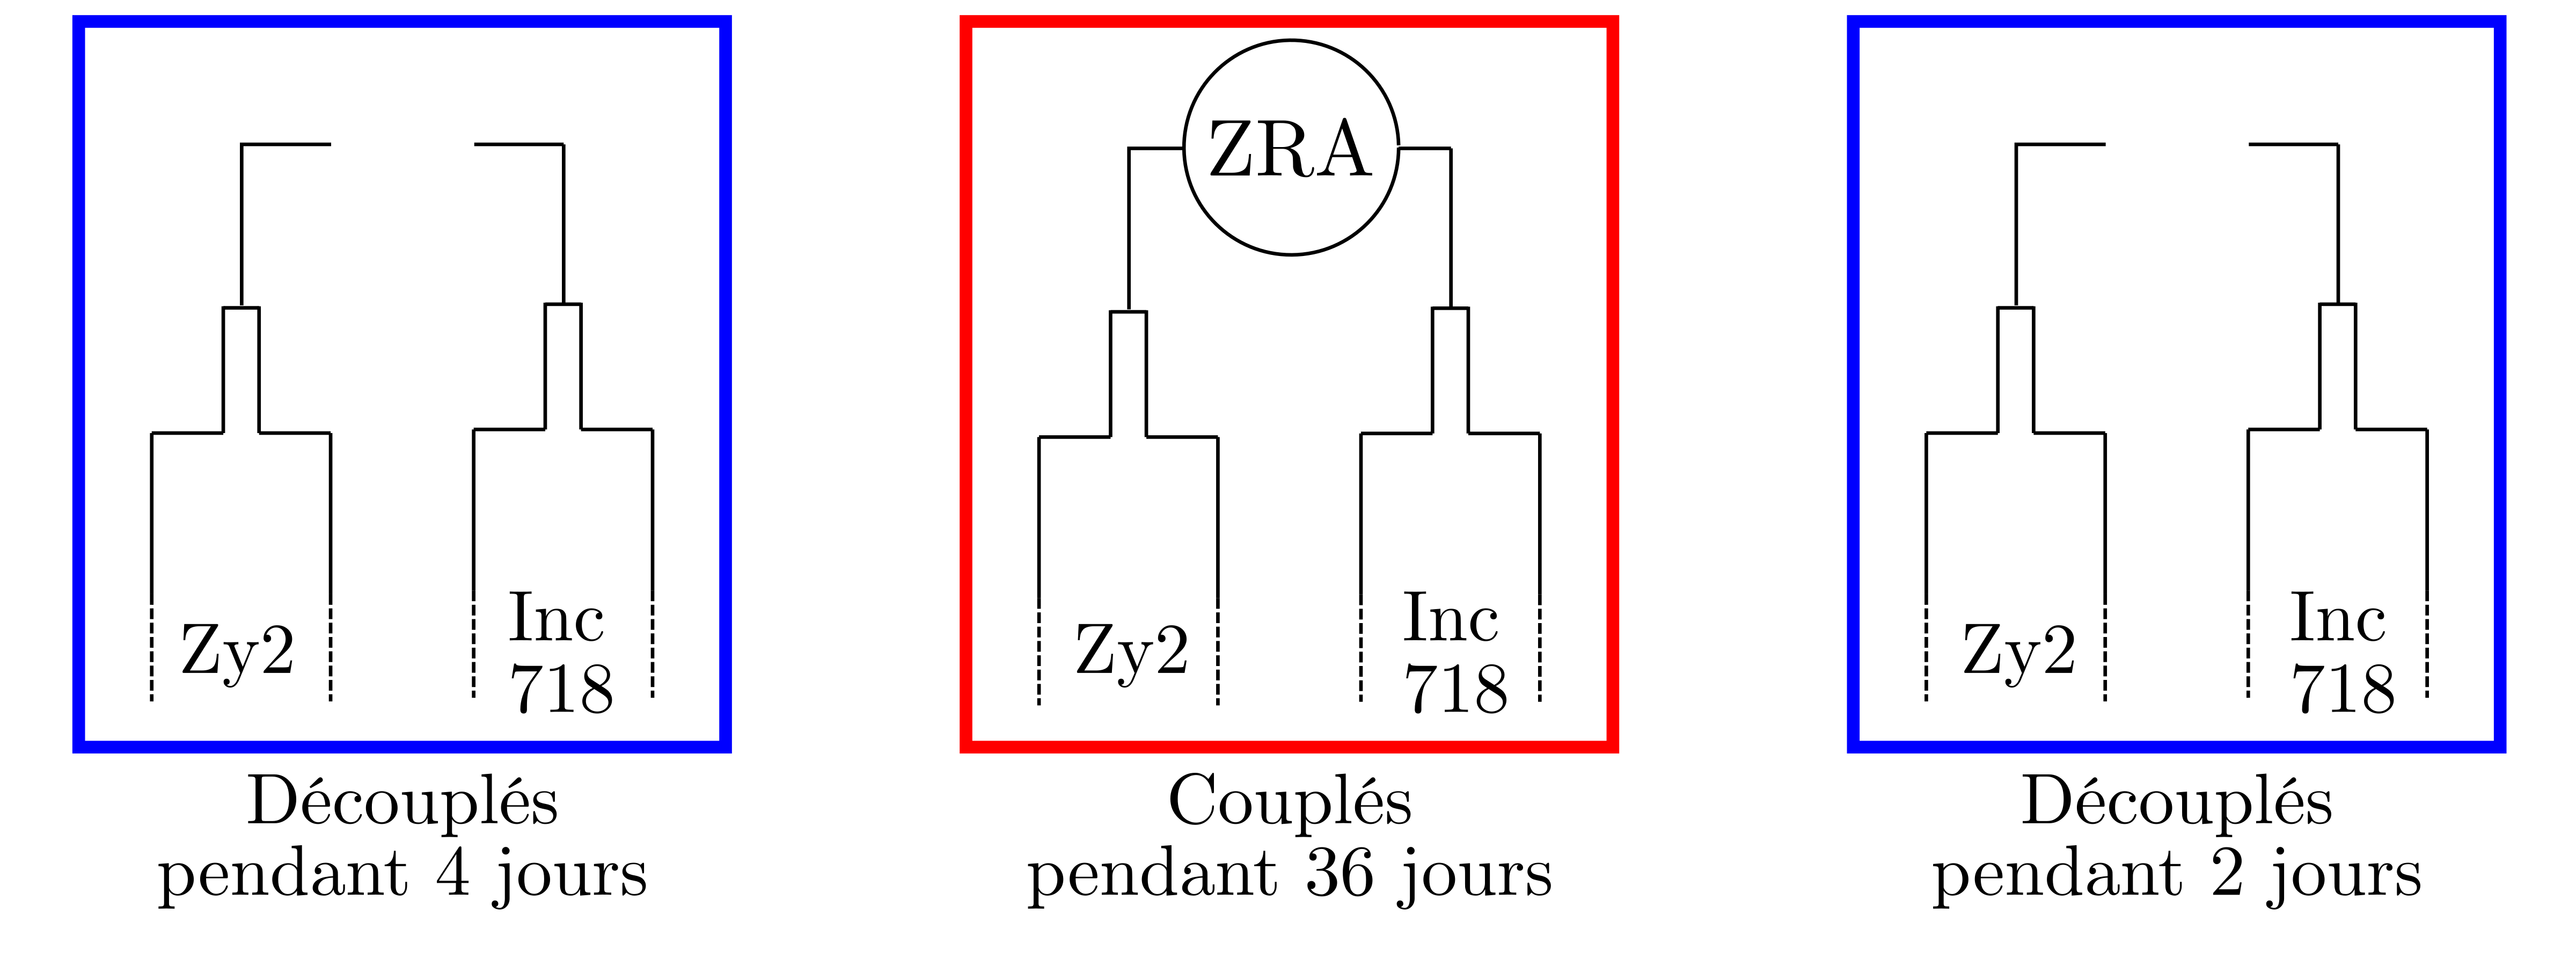
\includegraphics[width=0.85\textwidth]{140778-Coupling_Procedure.png}
        \caption{Représentation schématique du protocole des mesures de courant de couplage en micro-autoclave.}
        \label{fig:ch4_coupling_procedure}
    \end{figure}

    
    Dans la suite et pour des raisons de simplicité, nous ferons référence aux différents électrolytes selon la nomenclature suivante:

    \begin{itemize}
        \item électrolyte \water: électrolyte contenant seulement de l’eau ultra pure 
	    \item électrolyte \NaSO: électrolyte contenant de l’eau ultra pure et du sulfate de sodium
	    \item électrolyte \FeII: électrolyte contenant de l’eau ultra pure et des cations de fer (\FeII) 
	    \item électrolyte \ratio >2: électrolyte contenant de l’eau ultra pure et un mélange de cations (\FeII, \NiII\
            et \ZnII) dont le rapport molaire \ratio\ est supérieur à 2
        \item électrolyte  \ratio <2: électrolyte contenant de l’eau ultra pure et un mélange de cations (\FeII, \NiII\ et
        \ZnII), dont le rapport molaire \ratio\ est inférieur à 2
    \end{itemize}


    \subsection{Evolution des densités de courant de couplage}\label{subsec:current_density}

    La figure \ref{fig:ch4_jgal_coupling}
    montre l’évolution des densités de courant de couplage, j, des coupons rectangulaires de Zy2 
    dans les cinq électrolytes choisis.

    \begin{figure}[H]
        \centering
            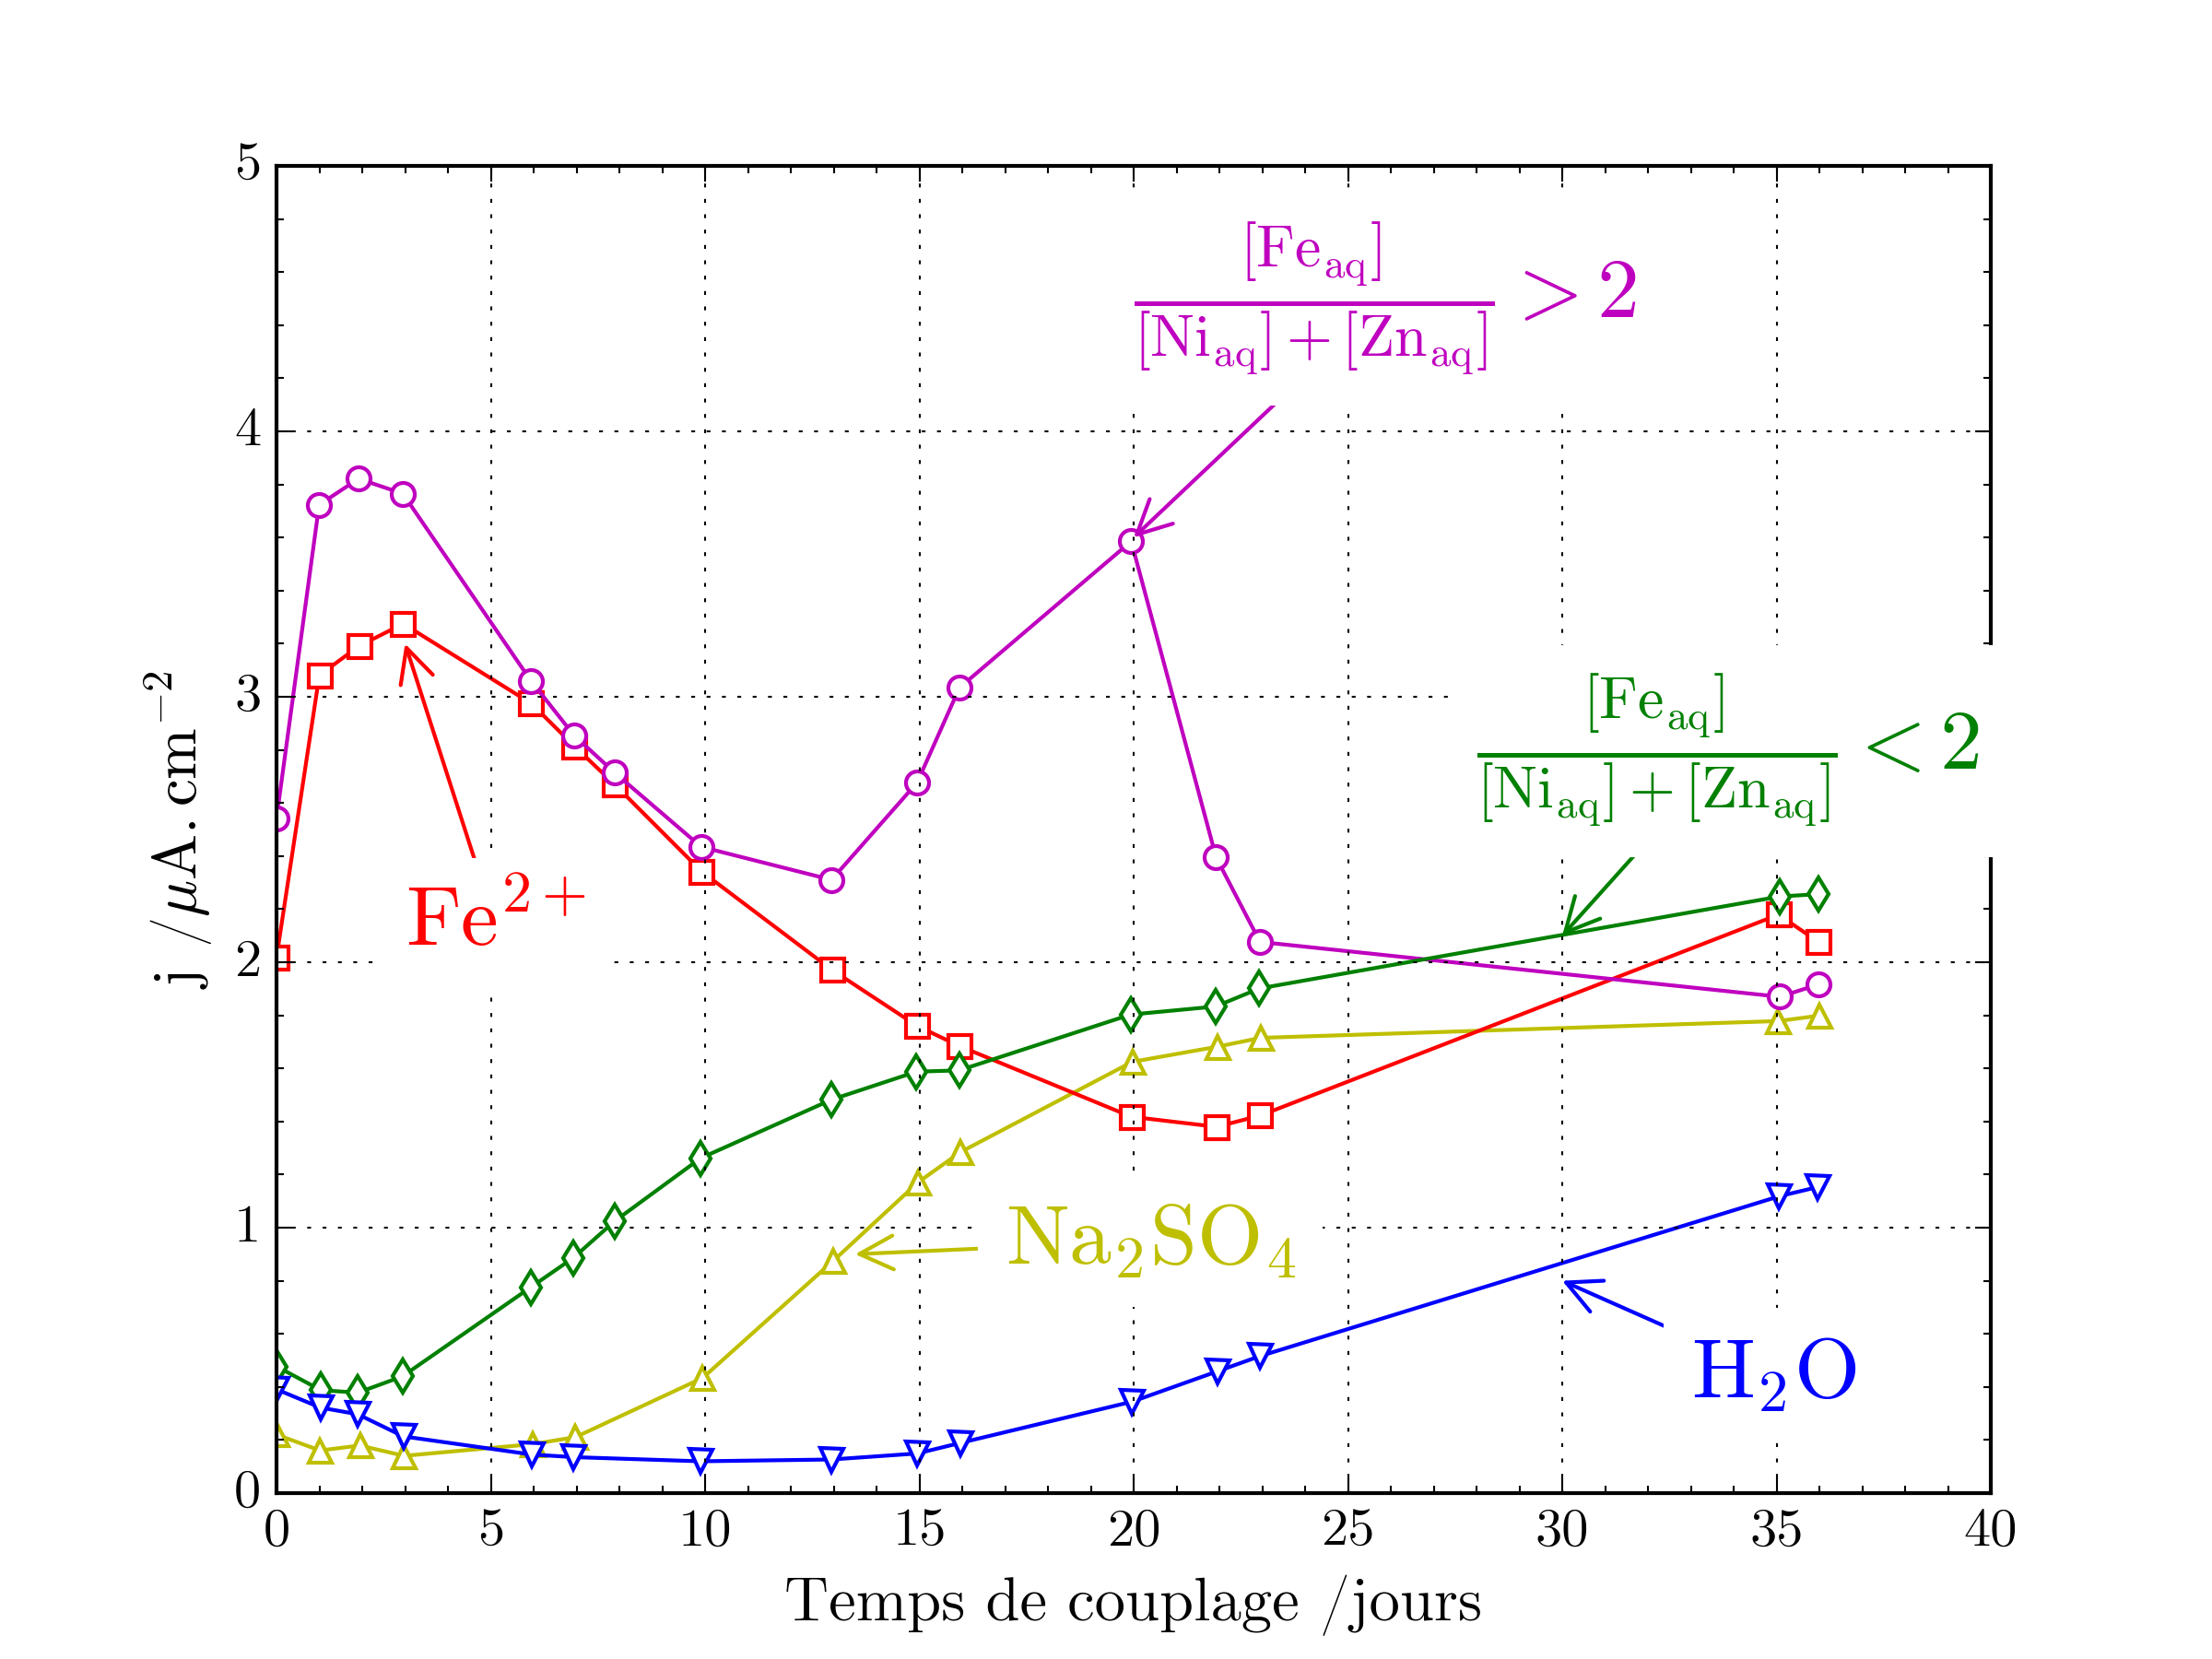
\includegraphics[width=\figwidth]{140778-Jgal_vs_Time.png}
        \caption{Evolution dans le temps des densités de courant de couplage pour les cinq électrolytes choisis.}
        \label{fig:ch4_jgal_coupling}
    \end{figure}

    Entre 0 et 10 jours de couplage, les densités de courant de couplage et leur évolution dans le
    temps apparaît dépendre significativement de l’électrolyte considéré. En effet, les électrolytes
    les plus chargés en cations de fer, c’est-à-dire l’électrolyte \FeII\ et l’électrolyte
    \ratio >2, présentent les densités de courant les plus élevées avec un maximum
    à 3.3 et \SI{3.8}{\micro\ampere\per\square\centi\meter}, respectivement. Ces densités de courant sont environ 10 fois plus élevées 
    que pour les trois autres. La présence de cations de fer en solution apparaît donc avoir un impact
    fort sur les densités de courant de couplage, et l’effet semble plus marqué lorsque les cations de 
    fer sont associés aux cations de nickel et de zinc tout ayant une concentration plus élevée que celles
    de ces derniers. L’électrolyte \ratio >2 présente même un second maximum de densité de courant
    de couplage à 20 jours de couplage.

    Au-delà d’environ 20 jours de couplage, pour tous les électrolytes excepté \water, les densités de courant de couplage
    semblent atteindre une valeur stable autour de \SI{2}{\micro\ampere\per\square\centi\meter}. Il faut mentionner que les micro-autoclaves sont fabriqués
    en alliage de nickel A600 et qu’ils sont donc susceptibles de relâcher des cations métalliques de fer et de nickel
    \citep{Sennour2010}.
    Il est donc plausible que les augmentations de densités de courant, observées pour les électrolytes
    \ratio <2, \NaSO\ et \water, soient liées à l’augmentation des concentrations en cations de fer et de nickel
    provenant majoritairement du relâchement des micro-autoclaves car la surface exposée de ces derniers est bien plus grande
    que celle des échantillons rectangulaires en Inc718.

    A l’issue des expériences de couplage en micro-autoclaves, les cinq électrolytes ont subi des prélèvements
    pour analyses par ICP--MS. Ces analyses ont montré que les concentrations finales en cations de fer et de
    nickel étaient de fait plus élevées que les concentrations de départ. En fin d’expérience, les cinq électrolytes
    contiennent des teneurs similaires en cations de fer et de nickel, soit environ \SI{1}{\ppm}. Les cations de zinc n’ont été
    retrouvés que dans les électrolytes qui en contenaient initialement, à hauteur de \SI{40}{\ppb} pour l’électrolyte correspondant
    à un rapport initial \ratio <2, et de \SI{25}{\ppb} pour l’autre. En considérant que le zinc peut également
    provenir du relâchement des micro-autoclaves, ce dernier aurait dû être retrouvé dans tous les électrolytes à l’issue
    de l’expérience. L’origine de l’augmentation de la concentration de zinc dans ces deux électrolytes n’a pas été déterminée.

    Une pollution au fluor a également été détectée à hauteur de \SI{10}{\ppm} pour les cinq électrolytes. La source de cette
    pollution a pu être identifiée, elle provient des supports en PEEK qui peuvent, selon les grades industriels, être plus ou
    moins chargés en PTFE. Cependant, le passage en solution des ions fluorures du PEEK n’est pas instantané, et il
    nous paraît
    raisonnable de penser que les valeurs de densités de courant mesurées entre 0 et 10 jours peuvent être considérées 
    comme représentatives des effets de la composition initiale chaque électrolyte.

    En prenant en compte l’augmentation de la concentration en cations de fer et de nickel dans tous les électrolytes, on
    peut donc raisonnablement suggérer que les fortes densités de courant, mesurées entre 0 et 10 jours, pour les électrolytes
    contenant des cations de fer seulement, ou des cations de fer associés à des cations de nickel et de zinc, avec un
    rapport molaire initial \ratio >2, sont majoritairement dues à un mécanisme impliquant les ions fer.
    De plus, la présence de cations de nickel et de zinc peut amplifier l’effet des cations de fer mais il n’est pas possible
    de discerner un effet du nickel et du zinc hors présence du fer. L’effet combiné des cations de fer, nickel et zinc, provenant
    du relâchement des micro-autoclaves, pourrait donc expliquer l’augmentation des densités de courant observées
    sur les électrolytes \ratio <2, \NaSO\ et \water\ après 10 jours de couplage.

    Ainsi, ces premiers résultats de mesures directes des courants de couplage suggèrent qu’un rapport 
    molaire \ratio >2 est néfaste pour la corrosion du Zy2, contrairement à ce que laissait
    penser le retour d’expérience de l’incident du réacteur KKL. Néanmoins, il faut garder à l’esprit que ce
    retour d’expérience concernait des événements en réacteur sous irradiation.

    
    \subsection{Epaisseurs des couches d’oxydation des alliages Zy2}\label{subsec:oxide_thickness}
    
    Afin de permettre d’apprécier l’influence du couplage galvanique
    sur l’épaisseur des couches d’oxydation formées sur l’alliage Zy2
    lors des expériences en micro-autoclaves décrites en \ref{subsec:exp_cond_MA}, ces épaisseurs
    ont été estimées à la fois sur les coupons rectangulaires (couplés) et sur
    les disques (non couplés, disposés au fond des micro-autoclaves).

    Pour ces derniers, l’épaisseur a été évaluée à partir de pesées avant et après expérience.
    Les gains de masses mesurés ont été convertis en épaisseur de zircone en utilisant
    le rapport de conversion défini au chapitre \ref{chap:ch1_bib} (\S \ref{subsec:oxidation_introduction}),
    soit \SI{15}{\milli\gram\per\square\deci\meter}
    par micron d’épaisseur de zircone. Le choix pour ces échantillons de la méthode par pesée
    a été dicté par la nécessité de pouvoir les caractériser ultérieurement en cellule HTP, interdisant
    la découpe des disques nécessaire aux mesures en microscopie électronique. 

    En revanche, les épaisseurs de zircone formée sur les coupons rectangulaires
    couplés de Zy2 ont été mesurées par microscopie électronique à balayage
    (\emph{MEB-FEG Zeiss Leo 1530}), à partir d’observations en coupe faites sur des
    découpes effectuées au milieu de la zone immergée des échantillons.
    Les épaisseurs ont été mesurées sur chacune des faces des coupons rectangulaires,
    c’est-à-dire le côté faisant face à l’Inc718 dénommé ici côté intérieur,
    et celui faisant face au corps du micro-autoclave, dénommé \emph{côté extérieur}. 

    L’ensemble des épaisseurs de zircone ainsi obtenues est rassemblé en figure \ref{fig:ch4_oxide_thickness}.

    \begin{figure}[H]
        \centering
        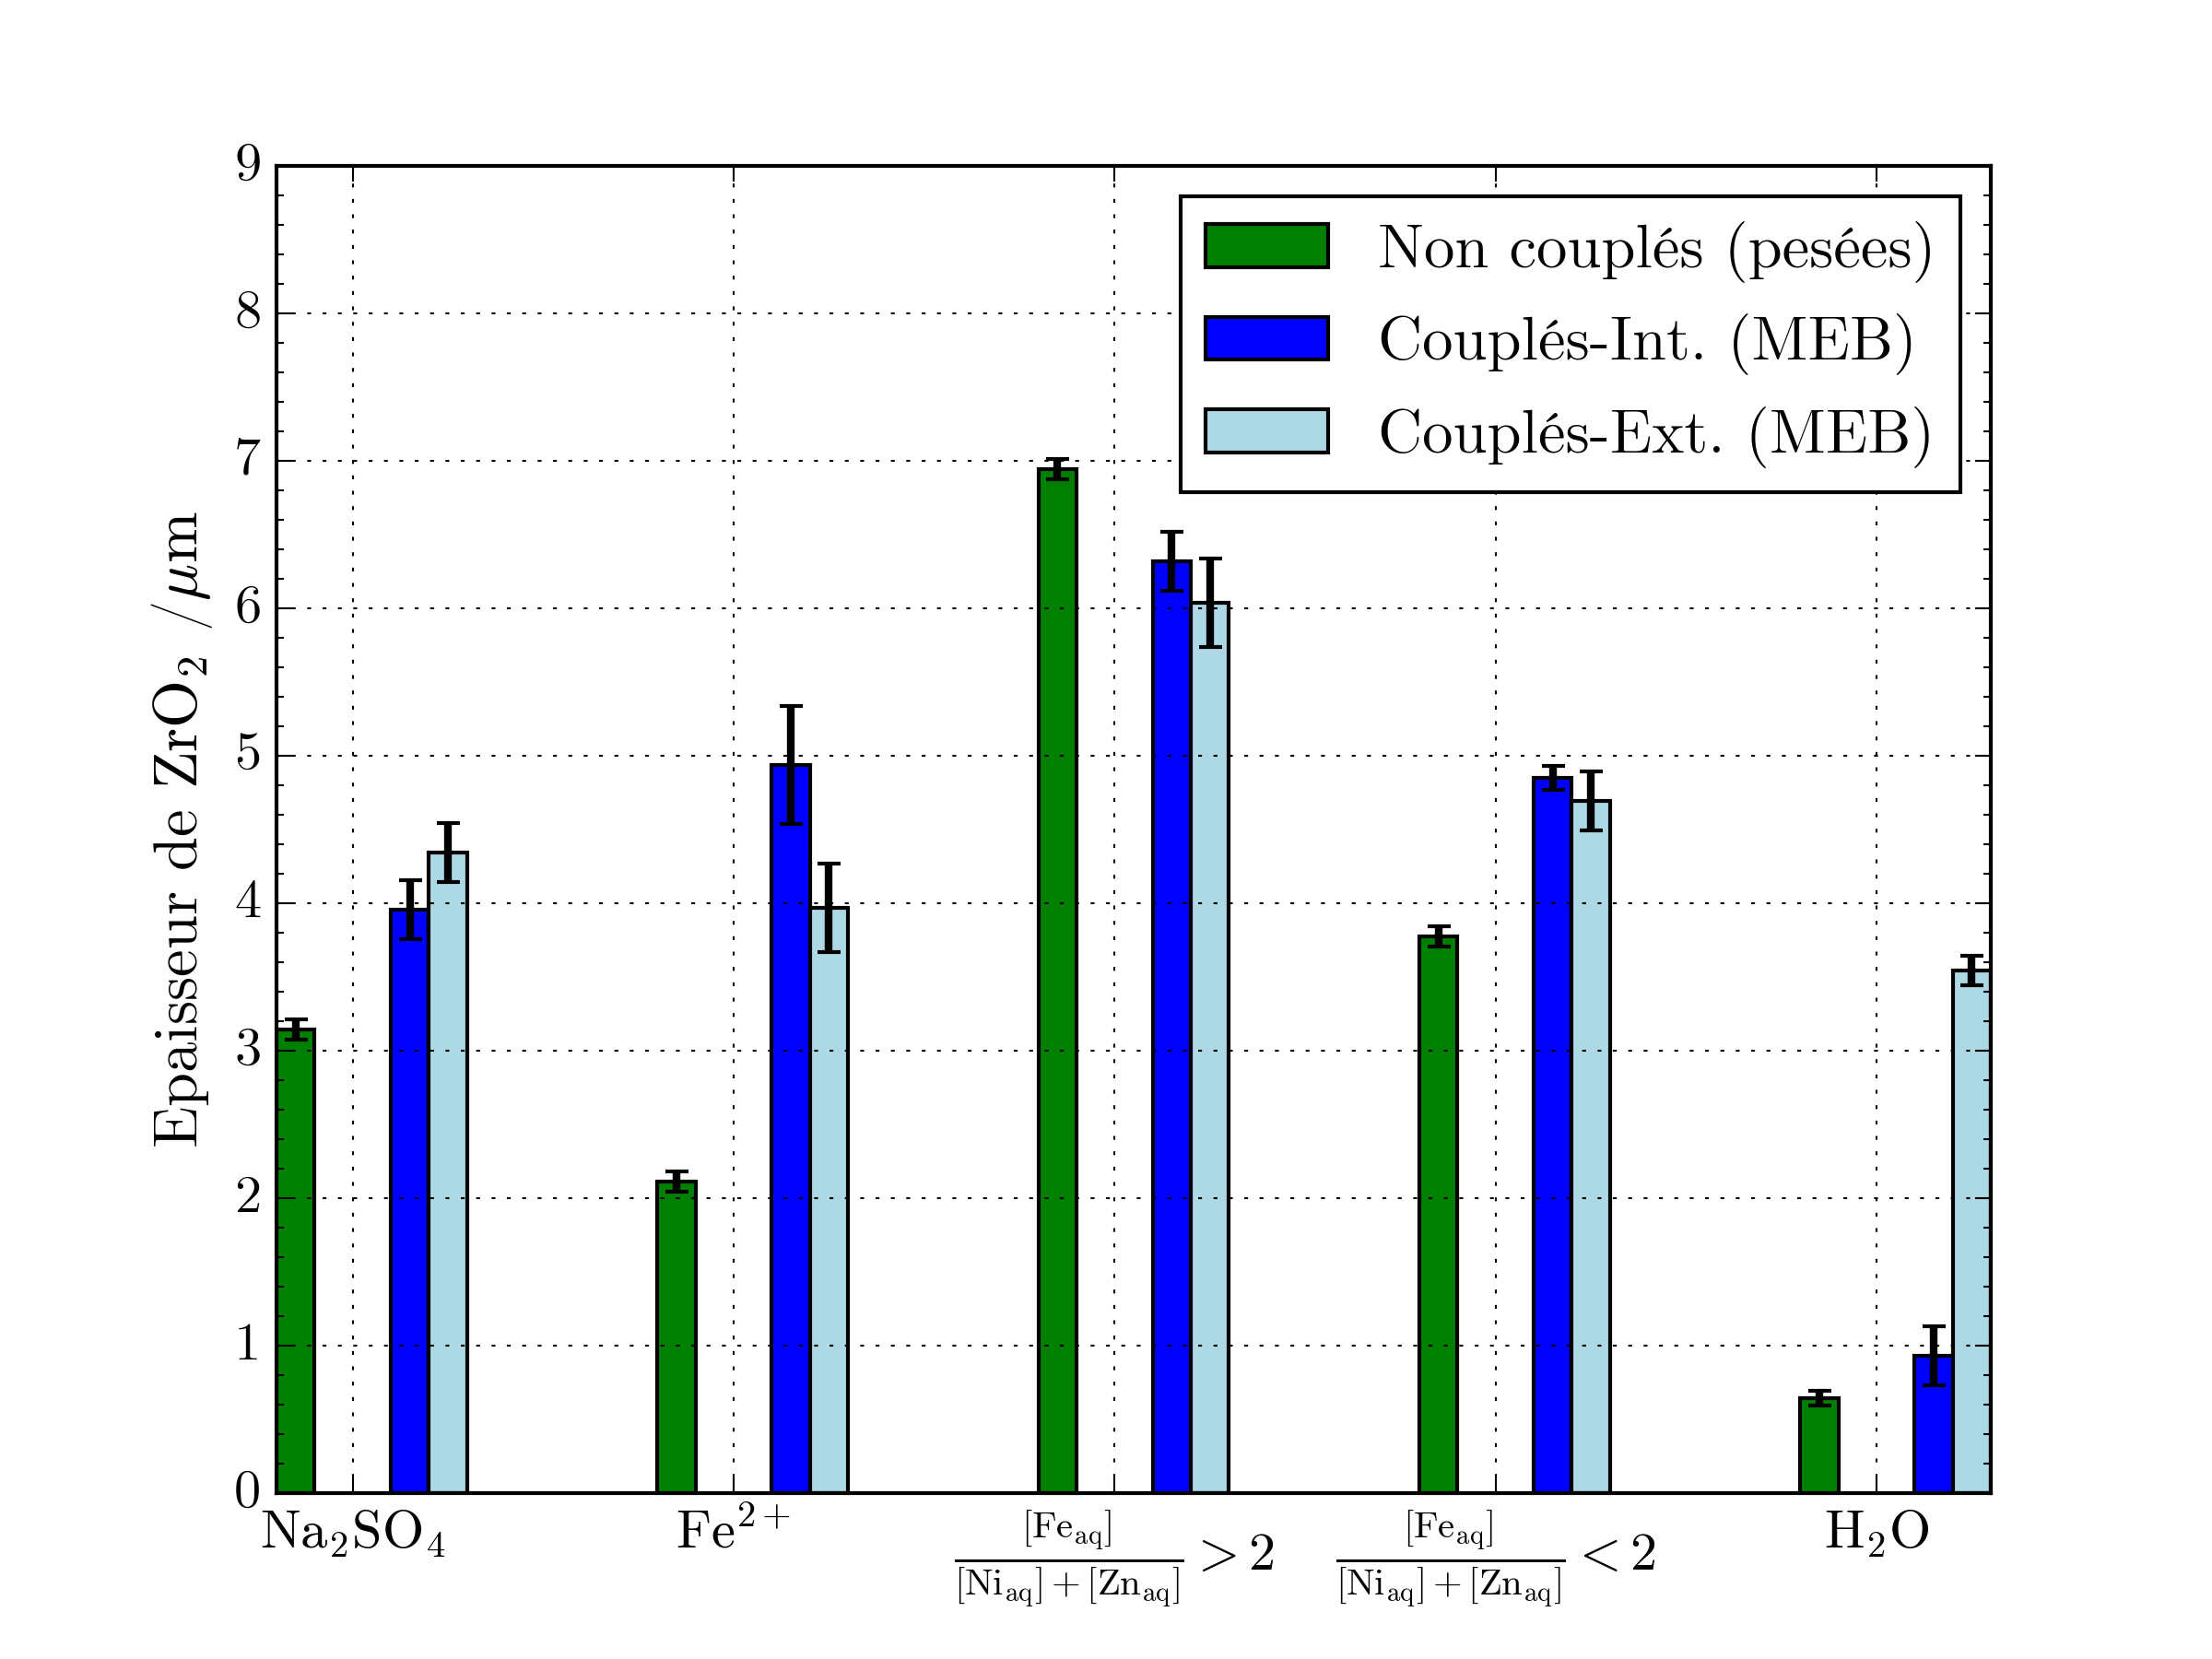
\includegraphics[width=\figwidth]{140778-Oxide_Thickness_Comparison.png}
        \caption{Epaisseurs de zircone mesurées par pesée sur les disques non couplés et par microscopie 
        électronique à balayage sur les coupons rectangulaires (côtés intérieur et extérieur).}
        \label{fig:ch4_oxide_thickness}
    \end{figure}


    Les épaisseurs mesurées sur les disques non couplés indiquent que
    les électrolytes contenant à la fois les cations de fer, nickel et
    zinc induisent les épaisseurs de zircone les plus importantes,
    soit \SI{6.9}{\micro\meter} lorsque le rapport molaire initial \ratio\ est
    supérieur à 2 et \SI{3.8}{\micro\meter} lorsque ce rapport est inférieur à 2.
    Ces valeurs sont très proches des épaisseurs mesurées sur les coupons
    rectangulaires couplés (côté intérieur : bâtonnets bleu foncé, côté extérieur : bâtonnets bleu clair).
    Il semble donc que pour ces deux électrolytes, le contact galvanique
    ait eu peu d’effet sur l’épaisseur de la couche d’oxydation. La même observation peut
    être faite pour l’électrolyte contenant \NaSO\, et pour l’eau pure, même si dans 
    ce dernier cas on relève une différence d’épaisseur entre les côtés intérieur et extérieur,
    différence dont l’origine n’a pu encore être expliquée.

    En revanche, lorsque l’électrolyte ne contient initialement que des cations fer,
    l’épaisseur de zircone mesurée sur les disques non couplés est environ deux fois
    moins élevée que celle mesurée sur les coupons rectangulaires couplés.
    
    Les résultats exposés ci-dessus suggèrent ainsi que l’existence d’un contact 
    galvanique n’a un effet notable sur la corrosion du Zy2 que lorsque l’électrolyte
    contient des cations de fer, comme l’indiquaient déjà les mesures de densités de
    courant de couplage. Egalement, ces dernières indiquaient que le courant de couplage
    le plus élevé était obtenu pour l’électrolyte ayant le rapport molaire initial
    \ratio\ supérieur à 2, et l’épaisseur de zircone mesurée dans
    ce cas est aussi la plus élevée. 
    
    Dans le but de mieux cerner l’effet des cations métalliques sur
    la nature des couches d’oxydes formées à la surface des échantillons
    de Zy2 et d’Inc718, des caractérisations photoélectrochimiques post-mortem
    ont été réalisées à température ambiante avec le dispositif PEC du laboratoire
    SIMaP. Seuls les coupons rectangulaires (couplés) ont été caractérisés afin d’éviter
    de découper les disques (non couplés) destinés à être caractérisés en cellule HTP.
    

    \subsection{Caractérisation PEC post-mortem des alliages Zy2 et Inc718 couplés et oxydés en
    micro-autoclave}\label{subsec:post_mortem_PEC}

    Comme exposé au chapitre \ref{chap:design} (\S \ref{subsec:ch3_principal_PEC} et \ref{subsec:ch3_experimentals}),
    les caractérisations
    PEC consistent à illuminer l’échantillon, utilisé comme
    électrode de travail dans une cellule électrochimique à trois électrodes et
    polarisé à un potentiel adéquat, avec une lumière monochromatique dont la longueur
    d’onde peut varier (généralement entre \SI{800}{\nano\meter} et \SI{200}{\nano\meter}), et à mesurer le
    photocourant induit par cette illumination dans l’échantillon. L’analyse des 
    photocourants mesurés en fonction du potentiel appliqué (photovoltammogrammes) 
    ou de l’énergie des photons (spectres en énergie de photocourants) permet d’obtenir
    des informations telles que la nature du dopage, le potentiel de bandes plates, et les
    énergies de bande interdite (gaps) des constituants semi-conducteurs de l’échantillon.
    Pour l’étude présentée dans ce paragraphe, nous nous sommes focalisés sur la mesure de
    spectres en énergie de photocourants, leur analyse permettant de détecter et d’identifier
    les phases d’oxydes présentes dans les couches d’oxydation. La méthode d’analyse des 
    spectres en énergie de photocourants développée dans l’équipe SIR de SIMaP et les
    perfectionnements qui y ont été apportés au cours de ce travail ont été décrites en
    détail au chapitre \ref{chap:design} (\S \ref{subsec:ch3_interpretation_PEC}).

    Typiquement, pour chacun des échantillons considérés, des spectres en 
    énergie de photocourants ont été mesurés. Chaque fois que cela a été possible,
    ces spectres ont été mesurés à plusieurs valeurs de potentiel appliqué, de manière
    à s’assurer que toutes les phases semi-conductrices constituant l’échantillon testé
    soient détectées, en tirant bénéfice des modifications de la situation de la charge
    d’espace des phases induites par les changements de potentiel appliqué. On notera
    cependant que le faible rapport signal/bruit des photocourants mesurés sur les
    échantillons de Zy2 ont nécessité des temps d’acquisition tels qu’il n’était pas
    raisonnable de mesurer plusieurs spectres pour chaque échantillon; seuls des spectres
    mesurés en polarisant l’échantillon au potentiel d’abandon ont donc été
    enregistrés pour les échantillons de Zy2.

    Avant caractérisation photoélectrochimique, le côté extérieur des échantillons
    a été poli au papier P1200 afin d’assurer un bon contact électrique avec le 
    circuit de mesure. Par conséquent, seule la couche d’oxydation formée sur le
    côté intérieur des coupons rectangulaires a été caractérisée. Les échantillons
    ont ensuite été rincés à l’éthanol puis à l’eau dans un bain à ultra-sons pendant
    10 minutes. Une solution de \NaSO\ à 0.1~M a été utilisée comme électrolyte de
    mesure, l’électrode de référence étant une électrode au sulfate mercureux (MSE)
    et la contre-électrode un coupon rectangulaire de platine.

    Signalons pour clore ce paragraphe que, faute de temps,
    les échantillons d’Inc718 et de Zy2 exposés dans l’électrolyte
    \NaSO\ n’ont pas été testés, la priorité ayant été donnée à l’évaluation
    de l’effet sur l’oxydation des échantillons de la présence dans l’électrolyte
    de cations fer, nickel et zinc.

    \subsubsection{Echantillon d'Inc718}\label{subsubsec:Inc718_samples}

    \paragraph{Spectre en énergie de photocourant au potentiel d'abandon}\label{parg:OCV_Iph}
    \mbox{}\\
    La figure \ref{fig:ch4_OCV_Iph_718} rassemble les spectres en énergie des modules de photocourants mesurés 
    au potentiel d’abandon sur le côté intérieur des coupons rectangulaires ainsi que les
    courbes obtenues par ajustement numérique des points expérimentaux. Pour souligner
    la qualité des résultats des ajustements numériques obtenus, nous avons également, 
    pour ce premier exemple, rassemblés en figure \ref{fig:ch4_OCV_ReImIph_718} les parties réelles et imaginaires 
    du photocourant complexe ainsi que les courbes correspondantes issues de l’ajustement 
    numérique des spectres.

    \begin{figure}[H]
        \centering
        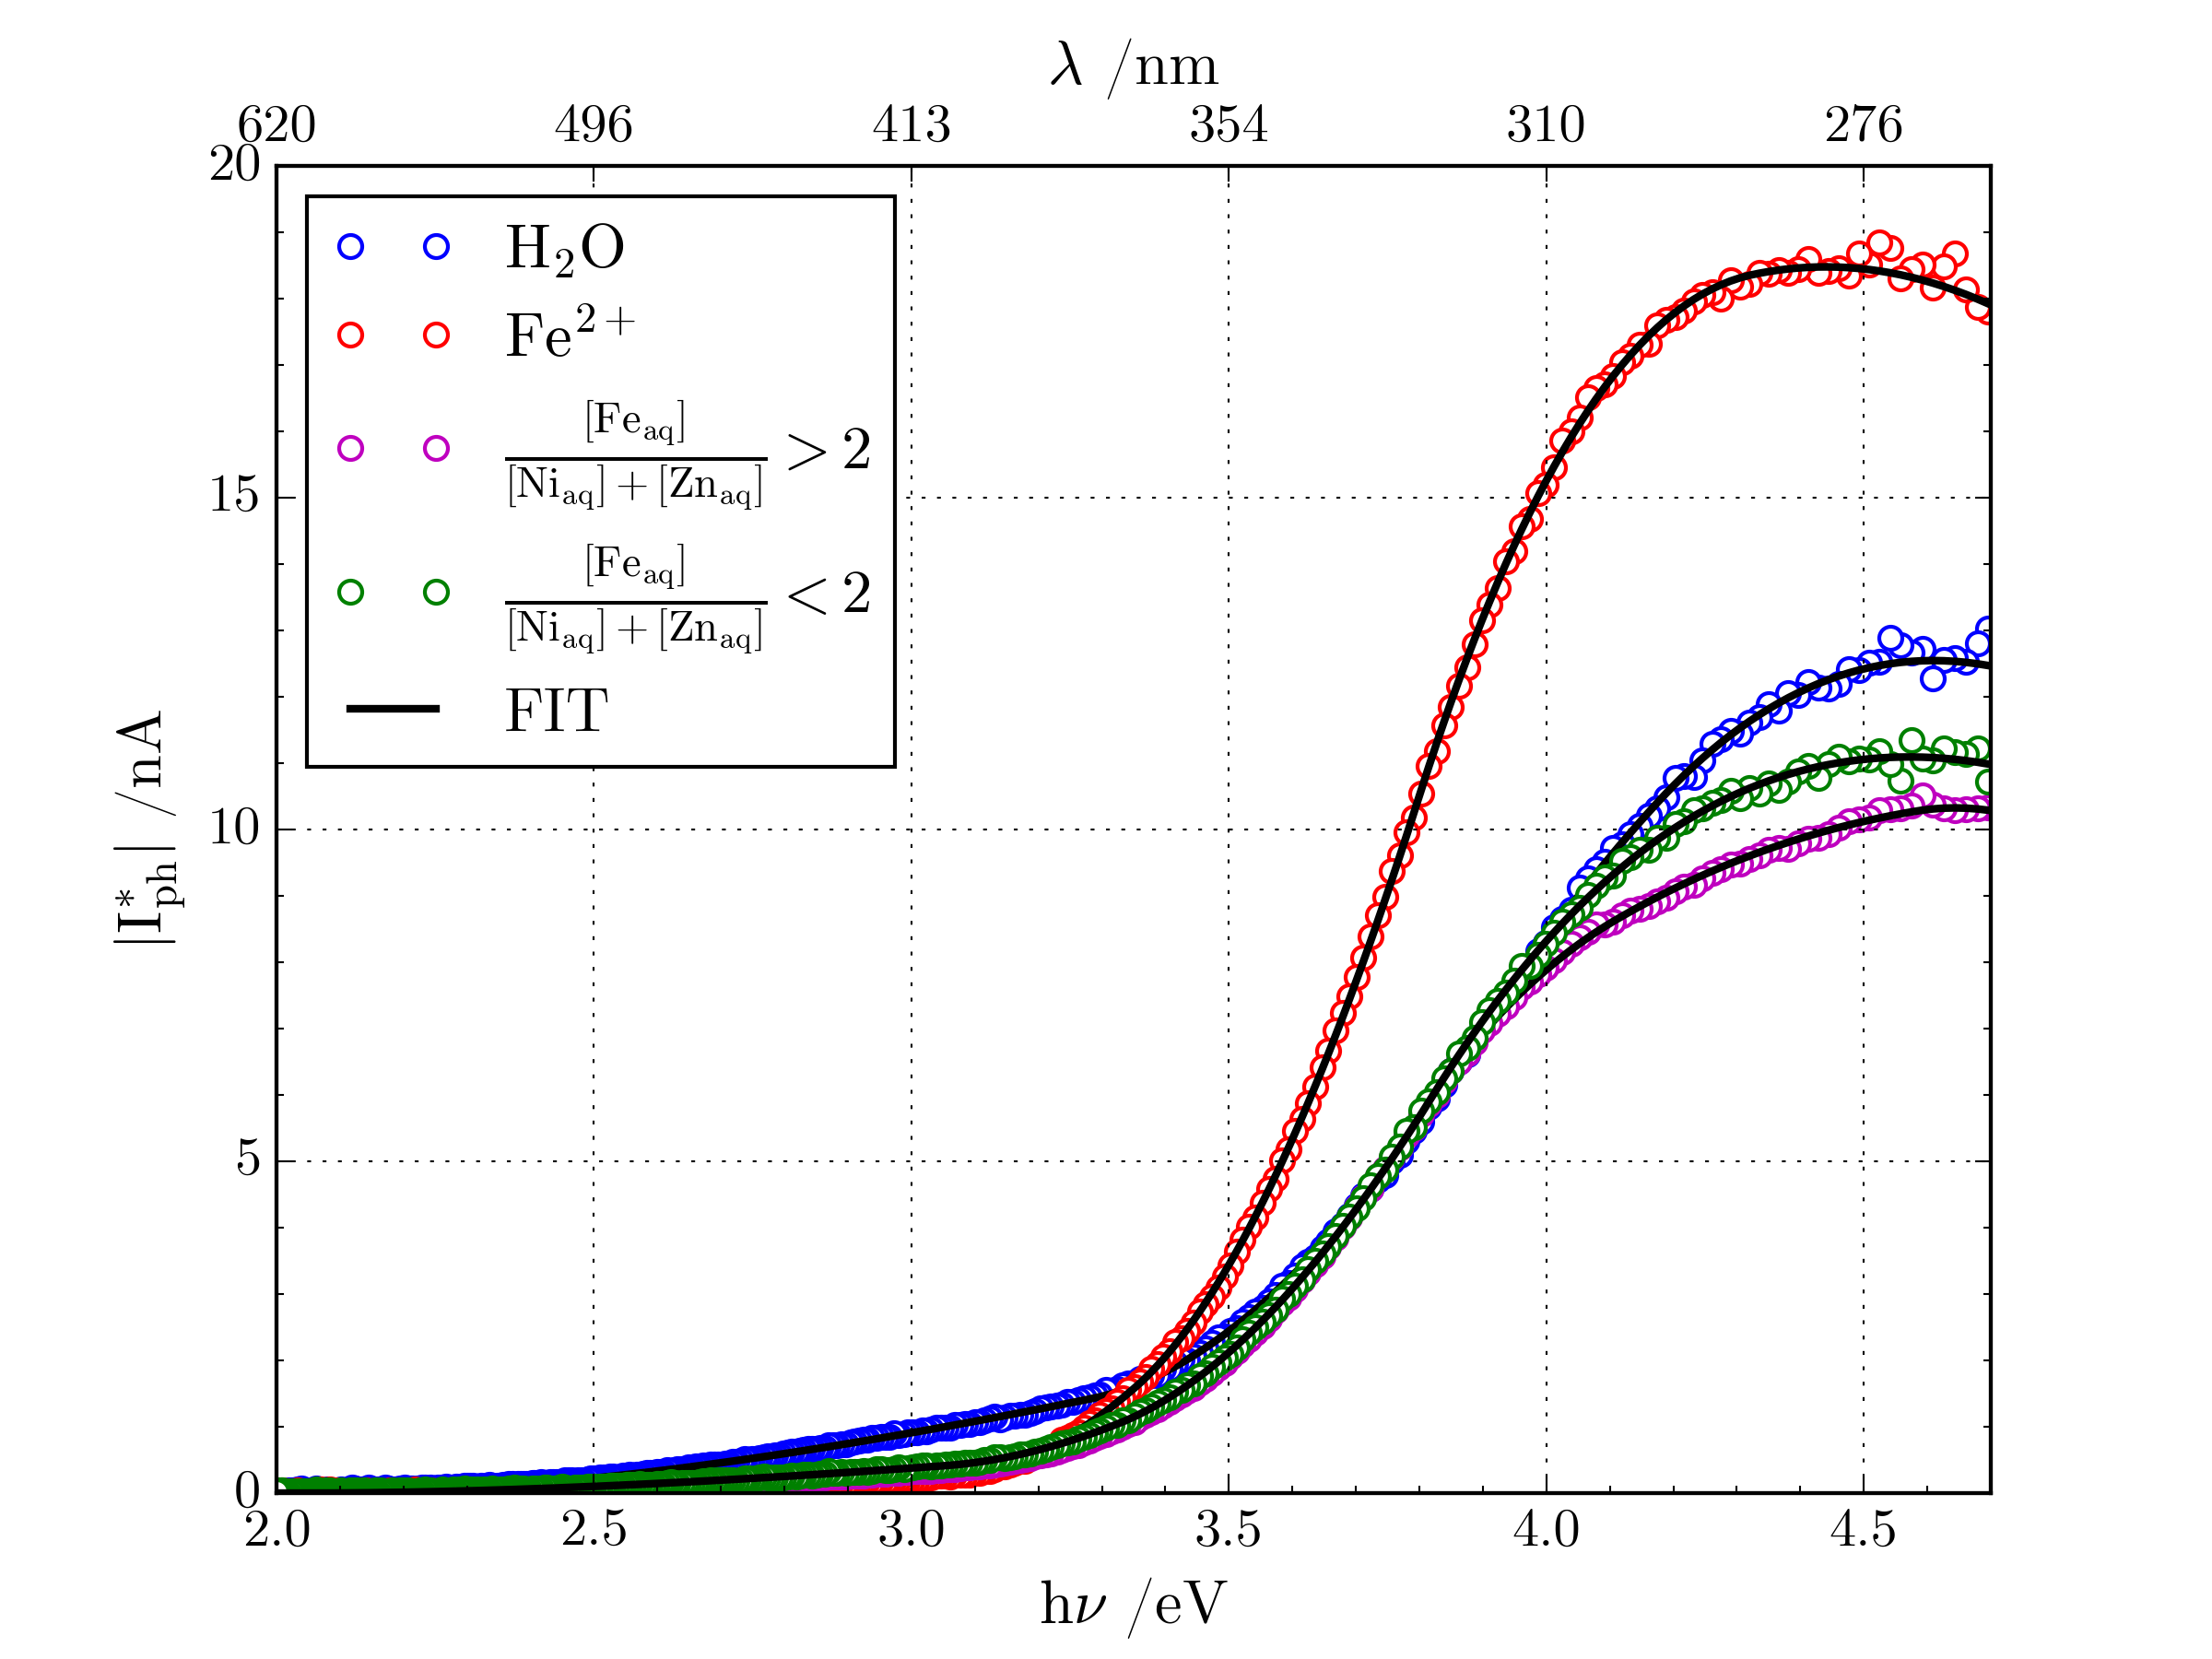
\includegraphics[width=\figwidth]{140778-PEC-Fit-Inc718-Iph.png}
        \caption{Spectres en énergie du module des photocourants complexes 
            mesurés sur le côté intérieur des coupons rectangulaires d’Inc718
            exposés à \SI{280}{\degreeCelsius} dans les différents électrolytes. "FIT" indique 
        les courbes obtenues par ajustement numérique.}
        \label{fig:ch4_OCV_Iph_718}
    \end{figure}


    \begin{figure}[H]
        \centering
        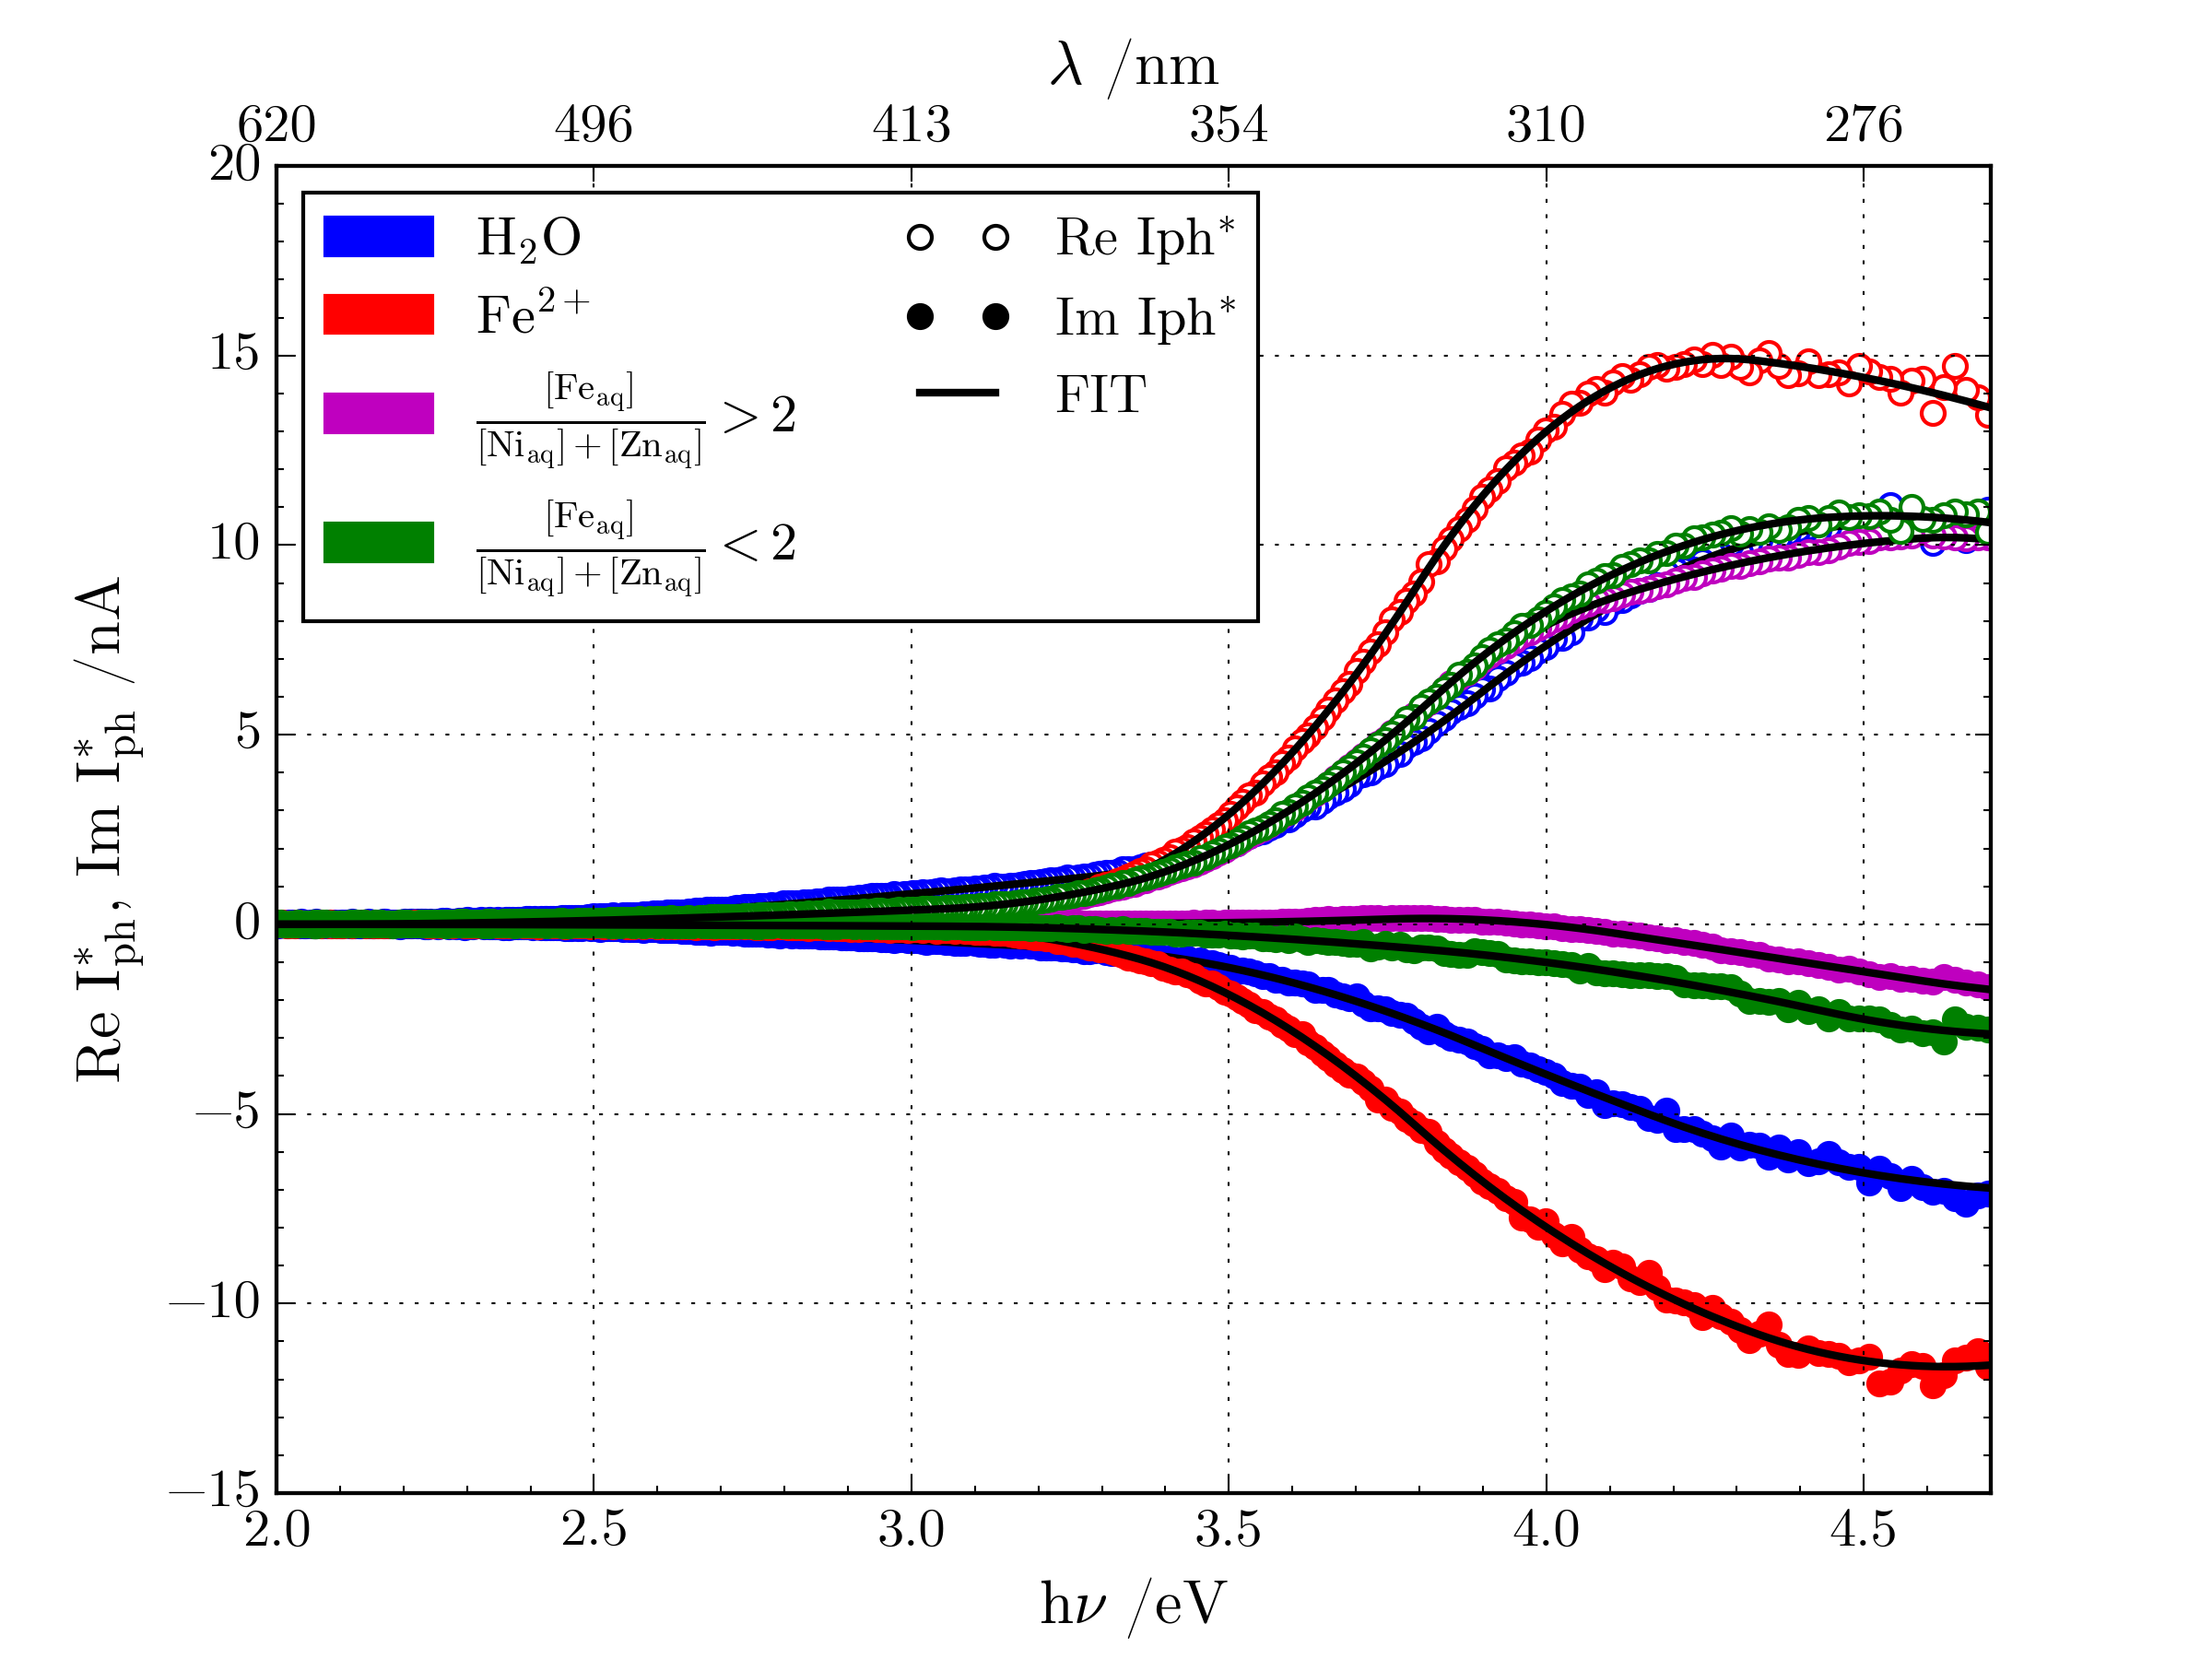
\includegraphics[width=\figwidth]{140778-PEC-Fit-Inc718-ReIm.png}
        \caption{Spectres en énergie des parties réelle et imaginaire des photocourants complexes mesurés sur le côté
            intérieur des coupons rectangulaires d’Inc718 exposés à \SI{280}{\degreeCelsius} dans les différents électrolytes. "FIT"
        indique les courbes obtenues par ajustement numérique.}
        \label{fig:ch4_OCV_ReImIph_718}
    \end{figure}

    Les valeurs de gaps, et les incertitudes correspondantes, déduites de ces ajustements numériques, pour les échantillons
    oxydés dans les quatre électrolytes retenus pour les caractérisations photo-électrochimiques post mortem, sont listées
    dans le tableau \ref{tab:ch4_band_gaps_fit_718}, et dans
    un souci de clarté, également représentées graphiquement en figure \ref{fig:ch4_Eg_718_graph}.


    Quel que soit l’électrolyte, deux gaps sont systématiquement présents, 
    à 2-2.1~eV et à 3.30-3.35~eV, signant très probablement la présence dans
    les couches d’hématite et de chromine, respectivement. Compte tenu de la
    littérature et de la concentration non négligeable de niobium dans l’Inc718 \citep{Liu1999}, le gap
    entre 3.76~eV et 3.90~eV pourrait raisonnablement être la signature de l’oxyde de
    niobium $Nb_2O_5$ \citep{LaMantia2010} provenant de l’oxydation des phases riches en niobium.
    
    Une contribution supplémentaire au photocourant est détectée au-delà de 4~eV, mais 
    sa valeur présente une plus grande dispersion d’un électrolyte à l’autre. Elle 
    pourrait être attribuée à un spinelle de type $Ni_{1-x}Fe_xCr_2O_4$ dont la largeur
    de bande interdite varierait avec ses teneurs en fer et nickel, elles-mêmes susceptibles
    de dépendre des teneurs initiales de l’électrolyte en fer et en nickel.
    
    On notera également que pour les couches formées en présence de cations de 
    fer dans les électrolytes, un gap supplémentaire est détecté (3.05 à 3.1~eV), qui
    ne l’est pas pour la couche formée en eau pure. Ce gap pourrait être attribué à 
    un spinelle de type $AB_2O_4$ telle que $FeCr_2O_4$. 

     \begin{table}[H]
         \begin{footnotesize}
        \centering
        \begin{tabular}{p{0.05\textwidth}|%
                        p{0.11\textwidth}%
                        p{0.18\textwidth}%
                        p{0.18\textwidth}%
                        p{0.11\textwidth}%
                        p{0.18\textwidth}%
                        }
            \toprule
            & \FeII & $\frac{[Fe_{aq}]}{[Ni_{aq}]+[Zn_{aq}]}$>2 & $\frac{[Fe_{aq}]}{[Ni_{aq}]+[Zn_{aq}]}$<2 & \water & Attributions \\ \midrule
            \rowcolor{lightgray}$E_{g,1}$ & 2 (TL) & 2.1 $\pm$ 0.4 & 2.1 $\pm$ 0.5 & 2.08 $\pm$ 0.08 & $Fe_2O_3$
            \citep{Benaboud2007,Wouters2004,Srisrual2009}\\ \hline
            $E_{g,2}$ & 3.1 $\pm$ 0.2 & 3.06 $\pm$ 0.05 & 3.05 $\pm$ 0.06 & & $FeCr_2O_4$ \citep{DiQuarto2000} \\ \hline
            \rowcolor{lightgray}$E_{g,3}$ & 3.35 $\pm$ 0.08 & 3.35 $\pm$ 0.04 & 3.33 $\pm$ 0.08 & 3.30 $\pm$ 0.02 & $Cr_2O_3$
            \citep{Benaboud2007,Wouters2004,Srisrual2009}, \citep{Wouters2008,Marchetti2010,Galerie2011,Henry2000}\\\hline
            $E_{g,4}$ & 3.80 $\pm$ 0.02 & 3.76 $\pm$ 0.02 & 3.82 $\pm$ 0.02 & 3.90 $\pm$ 0.04 & $Nb_2O_5$
            \citep{LaMantia2010}\\\hline
            \rowcolor{lightgray}$E_{g,5}$ & 4.33 $\pm$ 0.08 & 4.11 $\pm$ 0.05 & 4.4 $\pm$ 0.1 & 4.2 $\pm$ 0.2 & $Ni_{1-x}Fe_xCr_2O_4$
            \citep{Marchetti2010}\\ \hline
            $E_{g,6}$ &  & 4.58 $\pm$ 0.08 & & & $Ni_{1-x}Fe_xCr_2O_4$ \citep{Marchetti2010}\\ 
            \bottomrule
        \end{tabular}
        \caption{Valeurs de largeur de bande interdite ($E_{g,i}$ en eV) déduites des ajustements numériques des spectres en
        énergie de photocourants de la 
        figure \ref{fig:ch4_OCV_Iph_718} (la valeur marquée "TL" a été estimée par transformée linéaire) pour
    les couches formées dans les quatre électrolytes considérés.}
        \label{tab:ch4_band_gaps_fit_718}
    \end{footnotesize}
    \end{table}


    \begin{figure}[H]
        \centering
        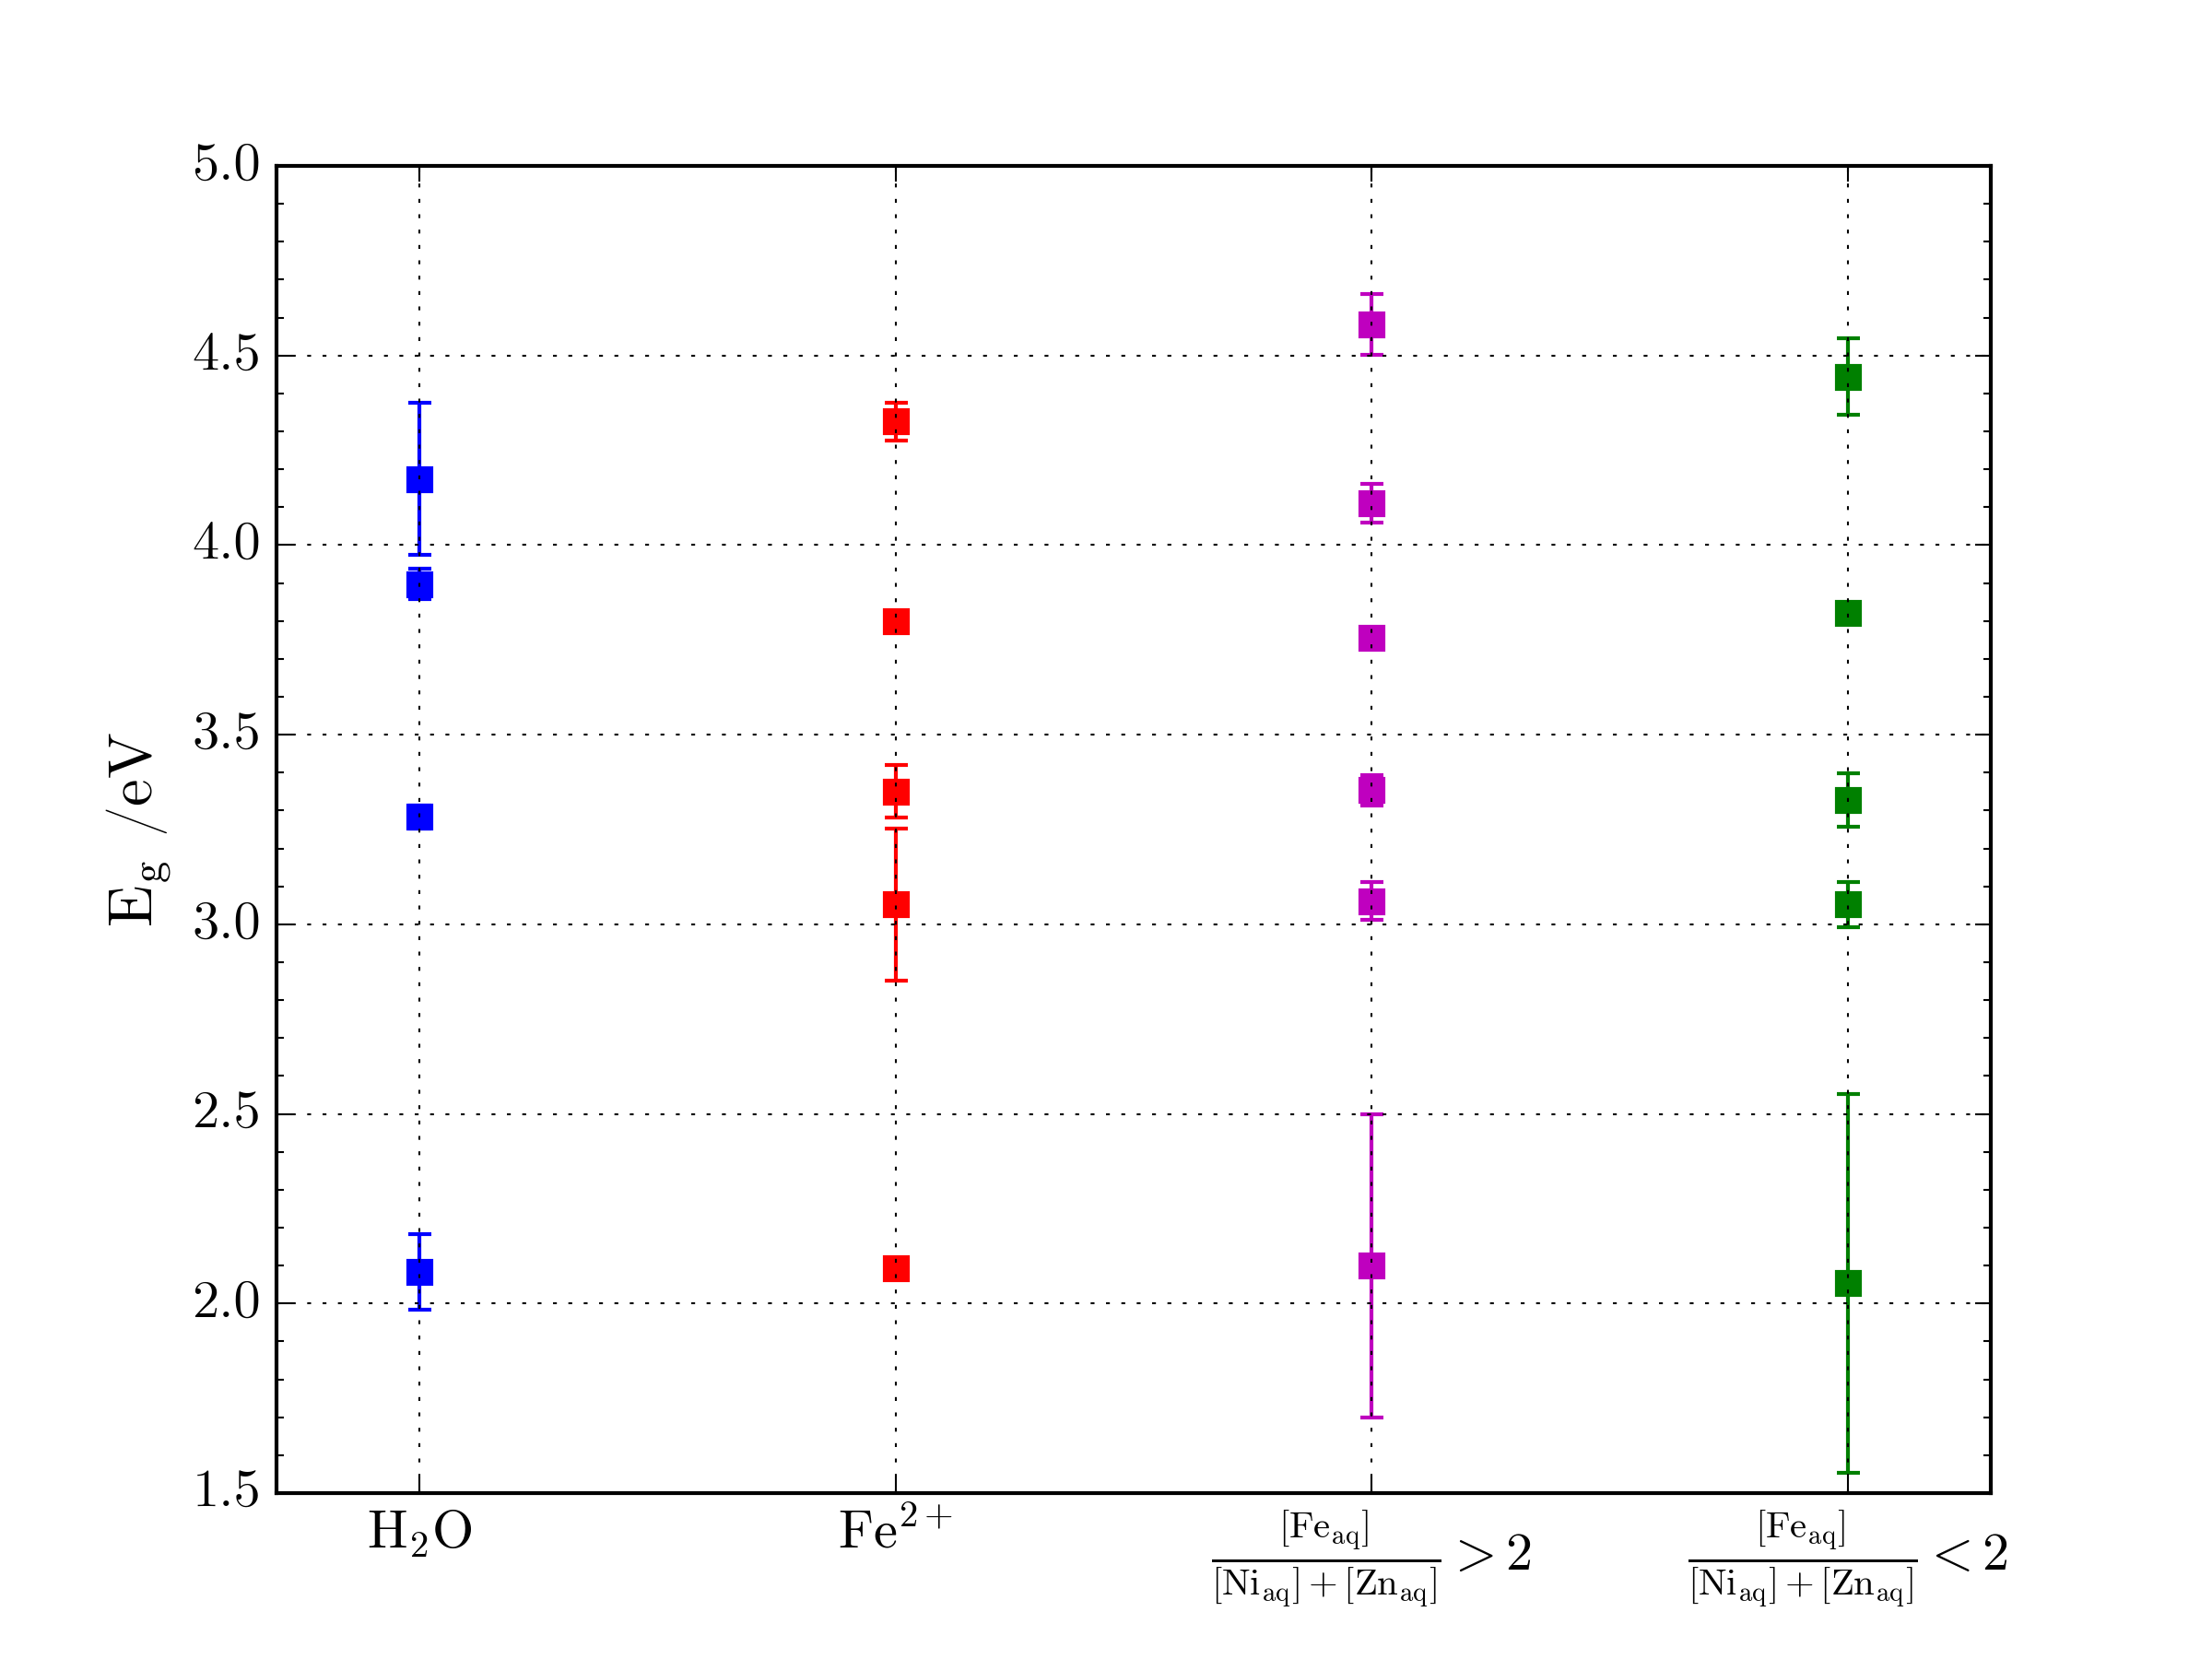
\includegraphics[width=\figwidth]{140778-PEC-Fit-Inc718-Eg_vs_chemistry.png}
        \caption{Représentation graphique des valeurs de largeur de bande interdite rassemblées au tableau \ref{tab:ch4_band_gaps_fit_718}.}
        \label{fig:ch4_Eg_718_graph}
    \end{figure}    


    Afin de s’assurer que toutes les contributions au photocourant ont pu être
    détectées en polarisant les échantillons
    au potentiel d’abandon, nous avons également analysé les spectres en énergie
    de photocourants mesurés à d’autres
    potentiels appliqués. Les résultats correspondants sont présentés ci-après.


    \paragraph{Spectres en énergie de photocourants à différents potentiels}\label{par:U_Iph}
    \mbox{}\\
    La figure \ref{fig:ch4_Iph_vs_U} rassemble les spectres en énergie de photocourants mesurés
    à différents potentiels pour chacun des échantillons d’Inc718 oxydé dans 
    l’un des quatre électrolytes sélectionnés. 

    On peut constater que, quel que soit l’échantillon, les amplitudes de 
    photocourants augmentent lorsque les potentiels appliqués deviennent plus
    anodiques (quelle que soit l’énergie de photons considérée), ce qui indique
    un comportement semiconducteur global de type \emph{n} pour chacune des couches. 

    Par ailleurs, pour un échantillon donné, les allures des spectres en énergie
    sont visuellement les mêmes à  tous les potentiels appliqués. Une normalisation
    des spectres, présentée en figure \ref{fig:ch4_Iph_vs_U_Normalized}, permet de constater que l’allure des spectres
    est réellement identique à tous les potentiels, et par conséquent de s’assurer que
    toutes les contributions au photocourant ont pu être détectées sur les spectres
    mesurés au potentiel d’abandon (\S \ref{subsubsec:Inc718_samples} \ref{parg:OCV_Iph}).


    \begin{figure}[H]
            \centering
            \begin{subfigure}[b]{0.48\textwidth}
                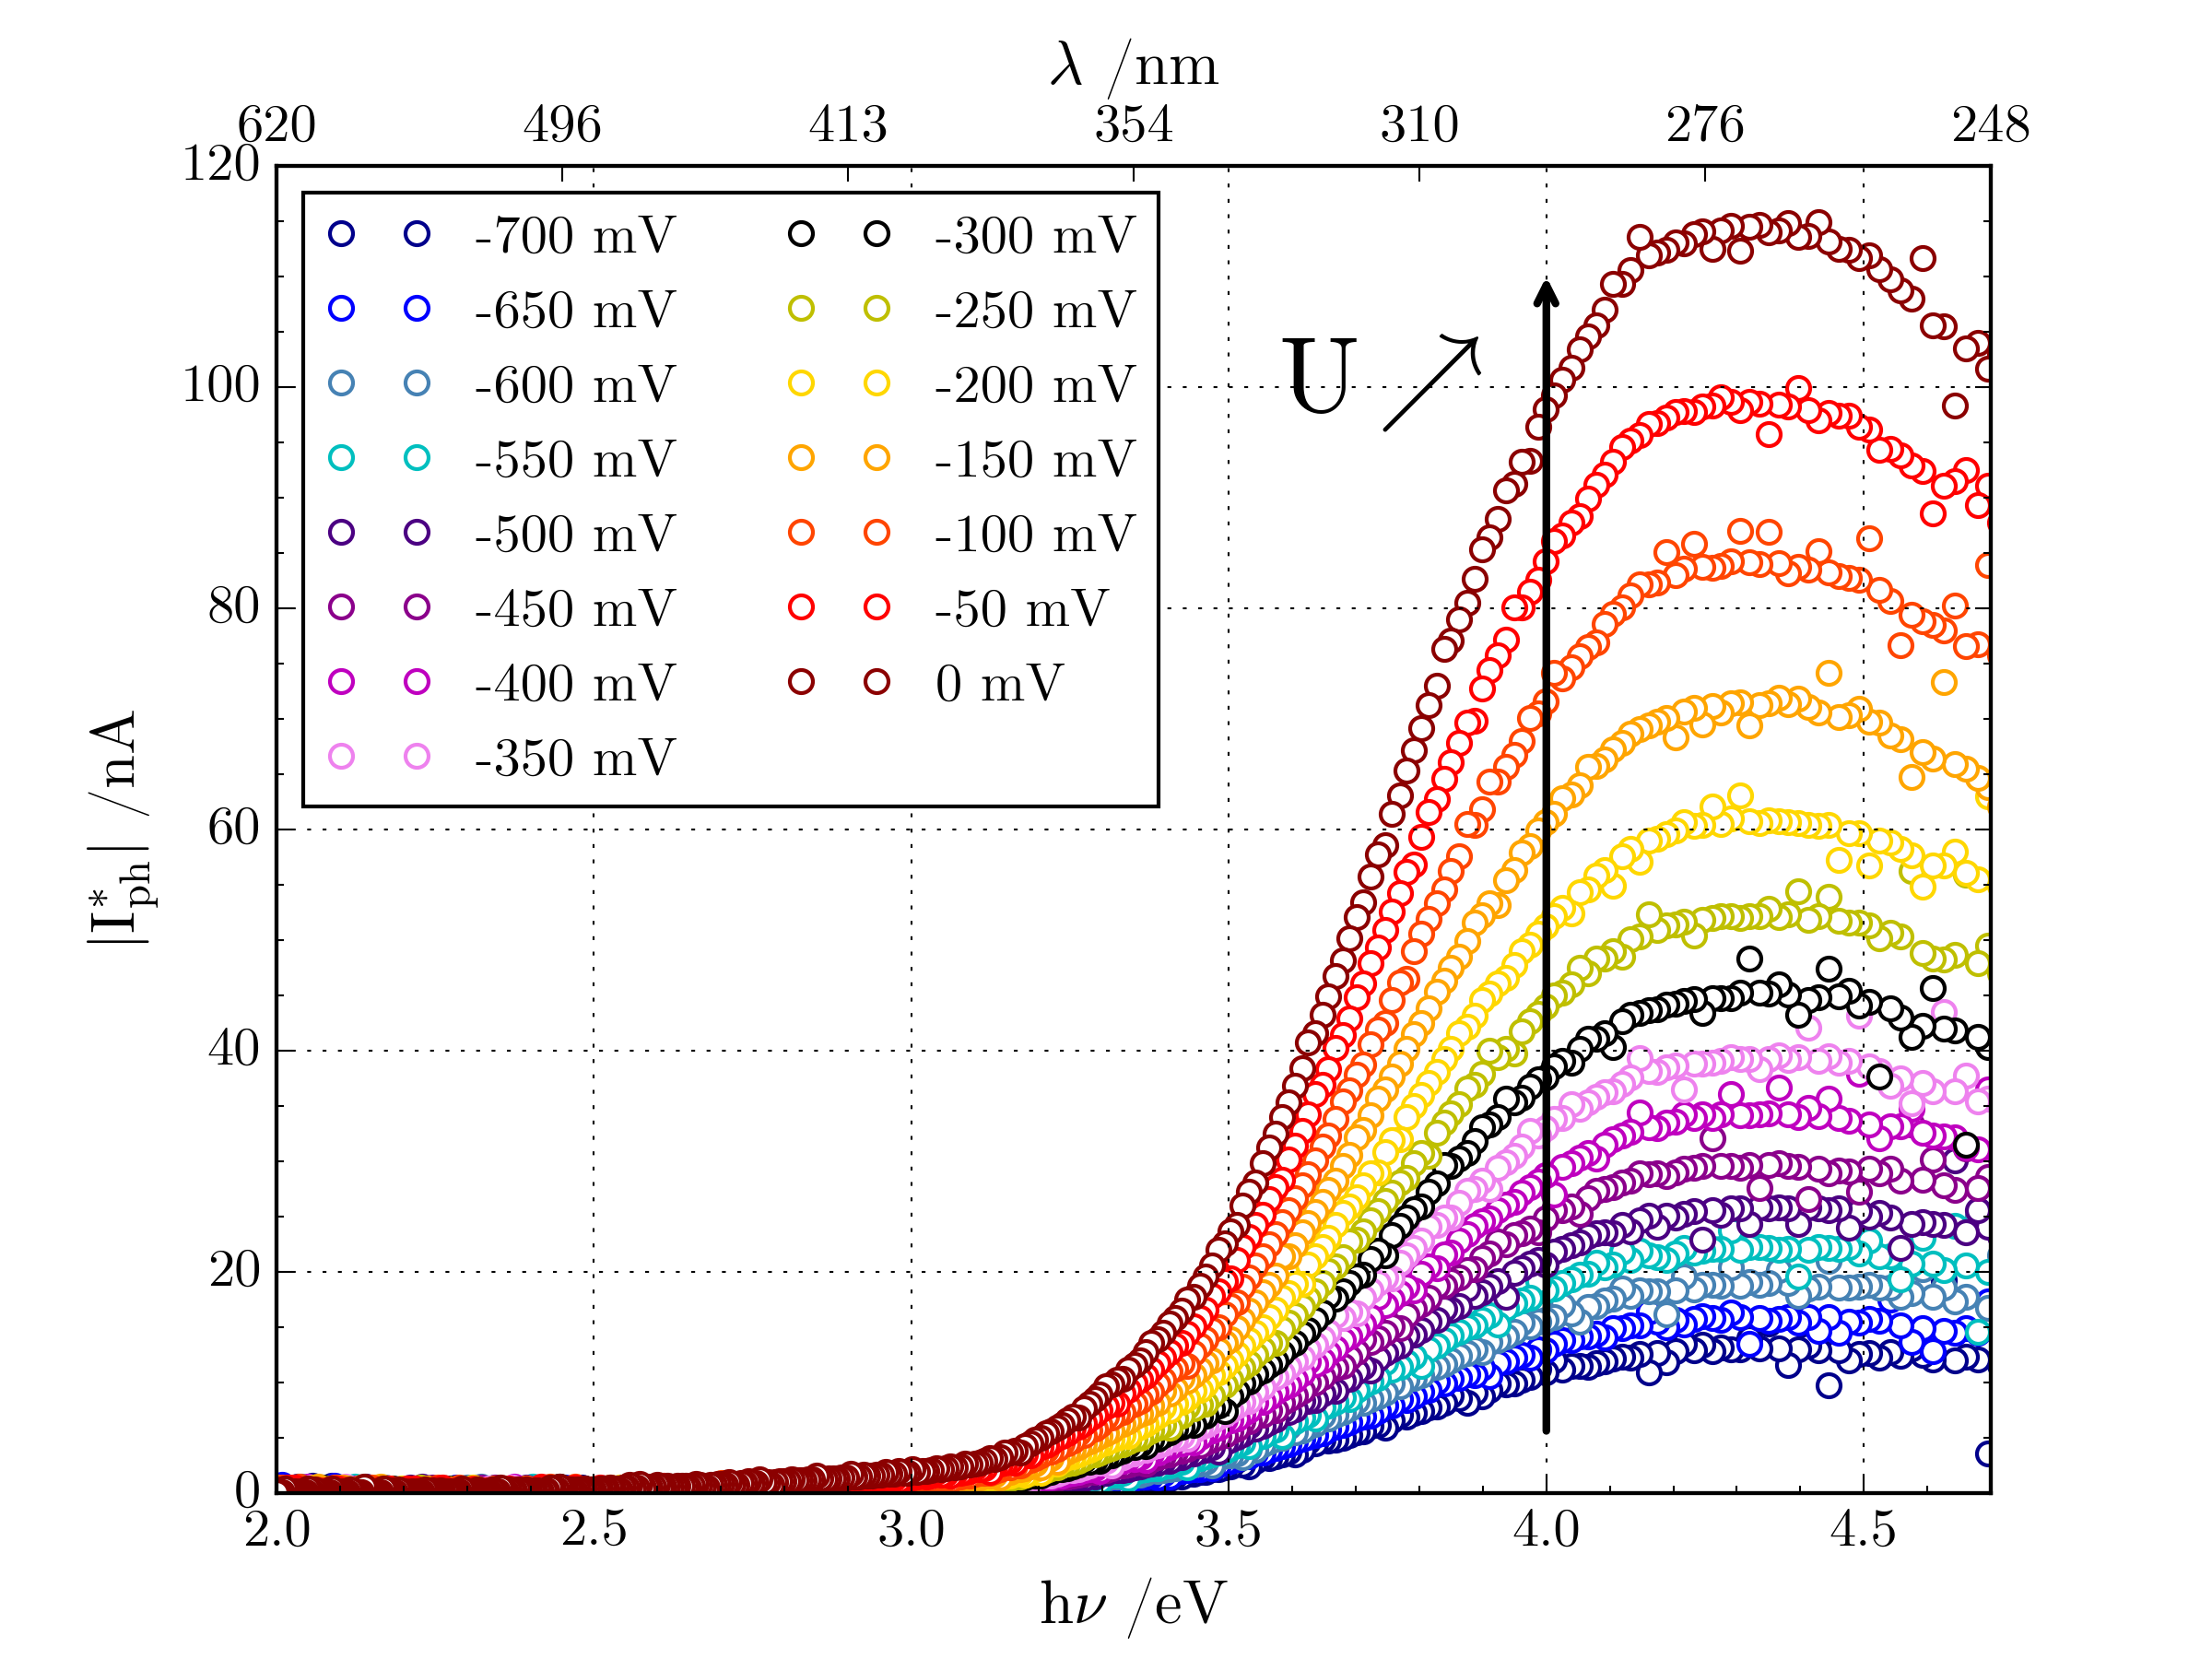
\includegraphics[width=\textwidth]{140778-PEC-X718-Iph-MA2-Polarization.png}
                \caption{}
                \label{}
            \end{subfigure}
            \begin{subfigure}[b]{0.48\textwidth}
                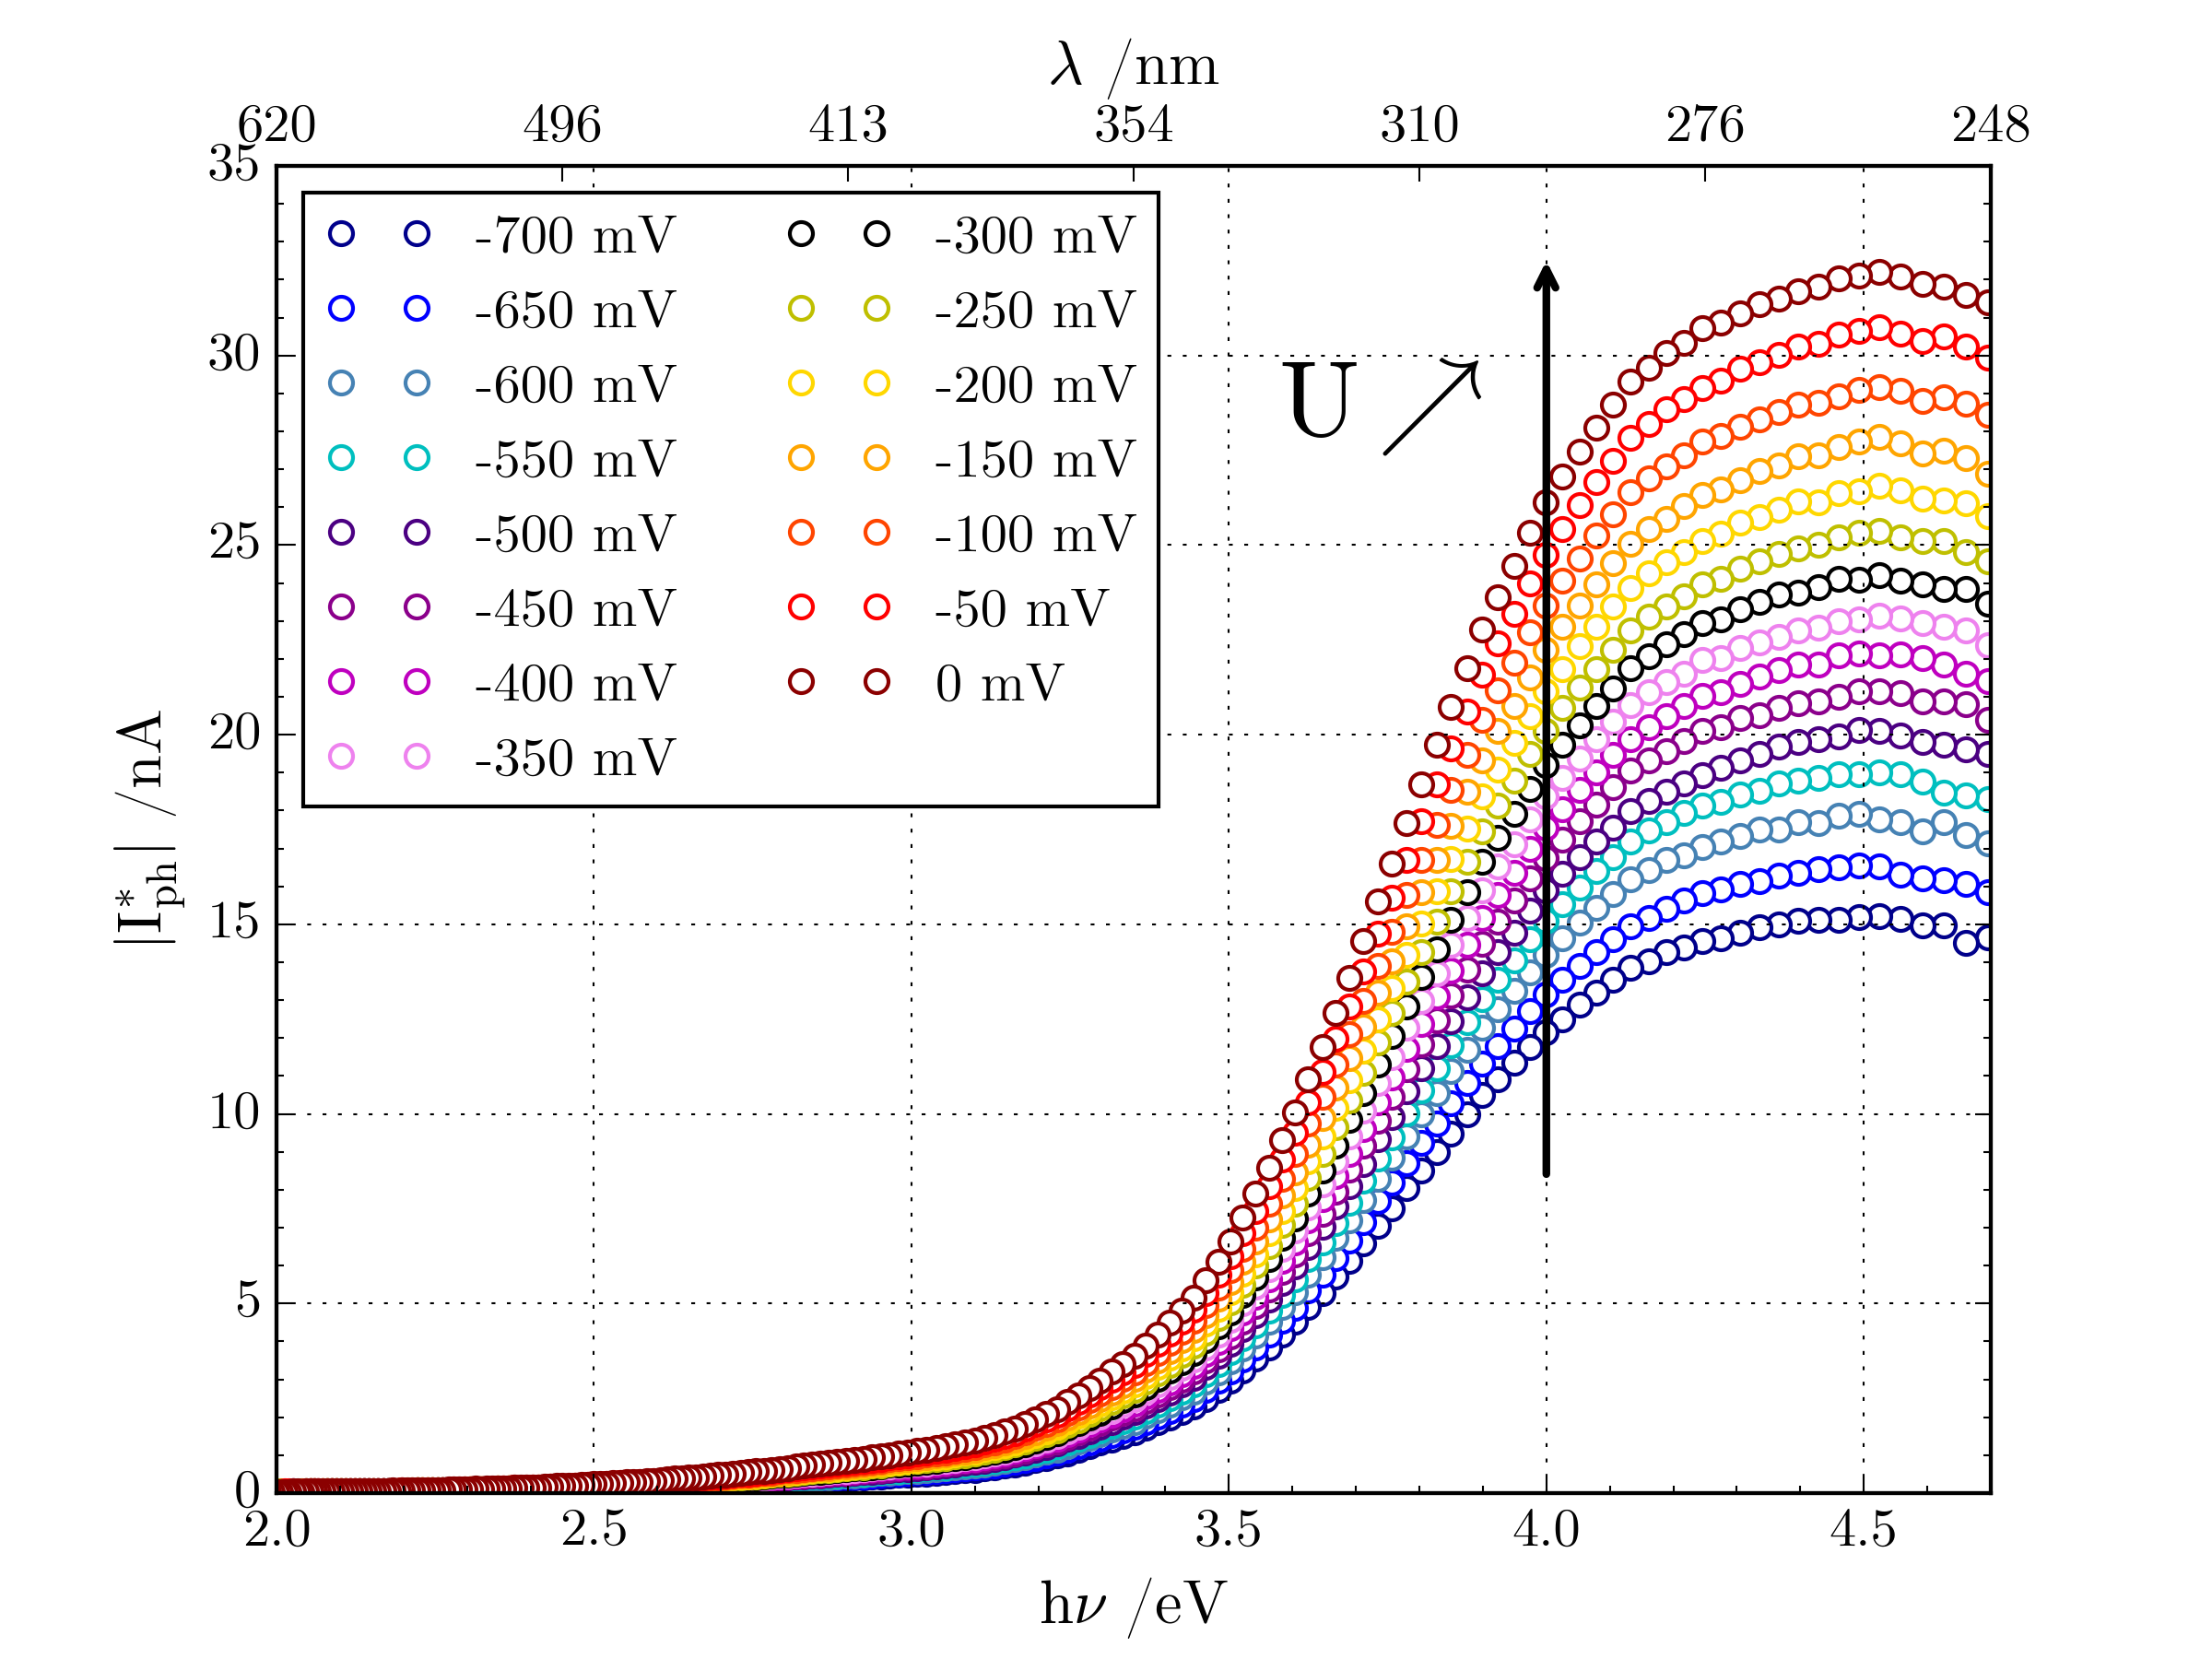
\includegraphics[width=\textwidth]{140778-PEC-X718-Iph-MA3-Polarization.png}
                \caption{}
                \label{}
            \end{subfigure}
            \begin{subfigure}[b]{0.48\textwidth}
                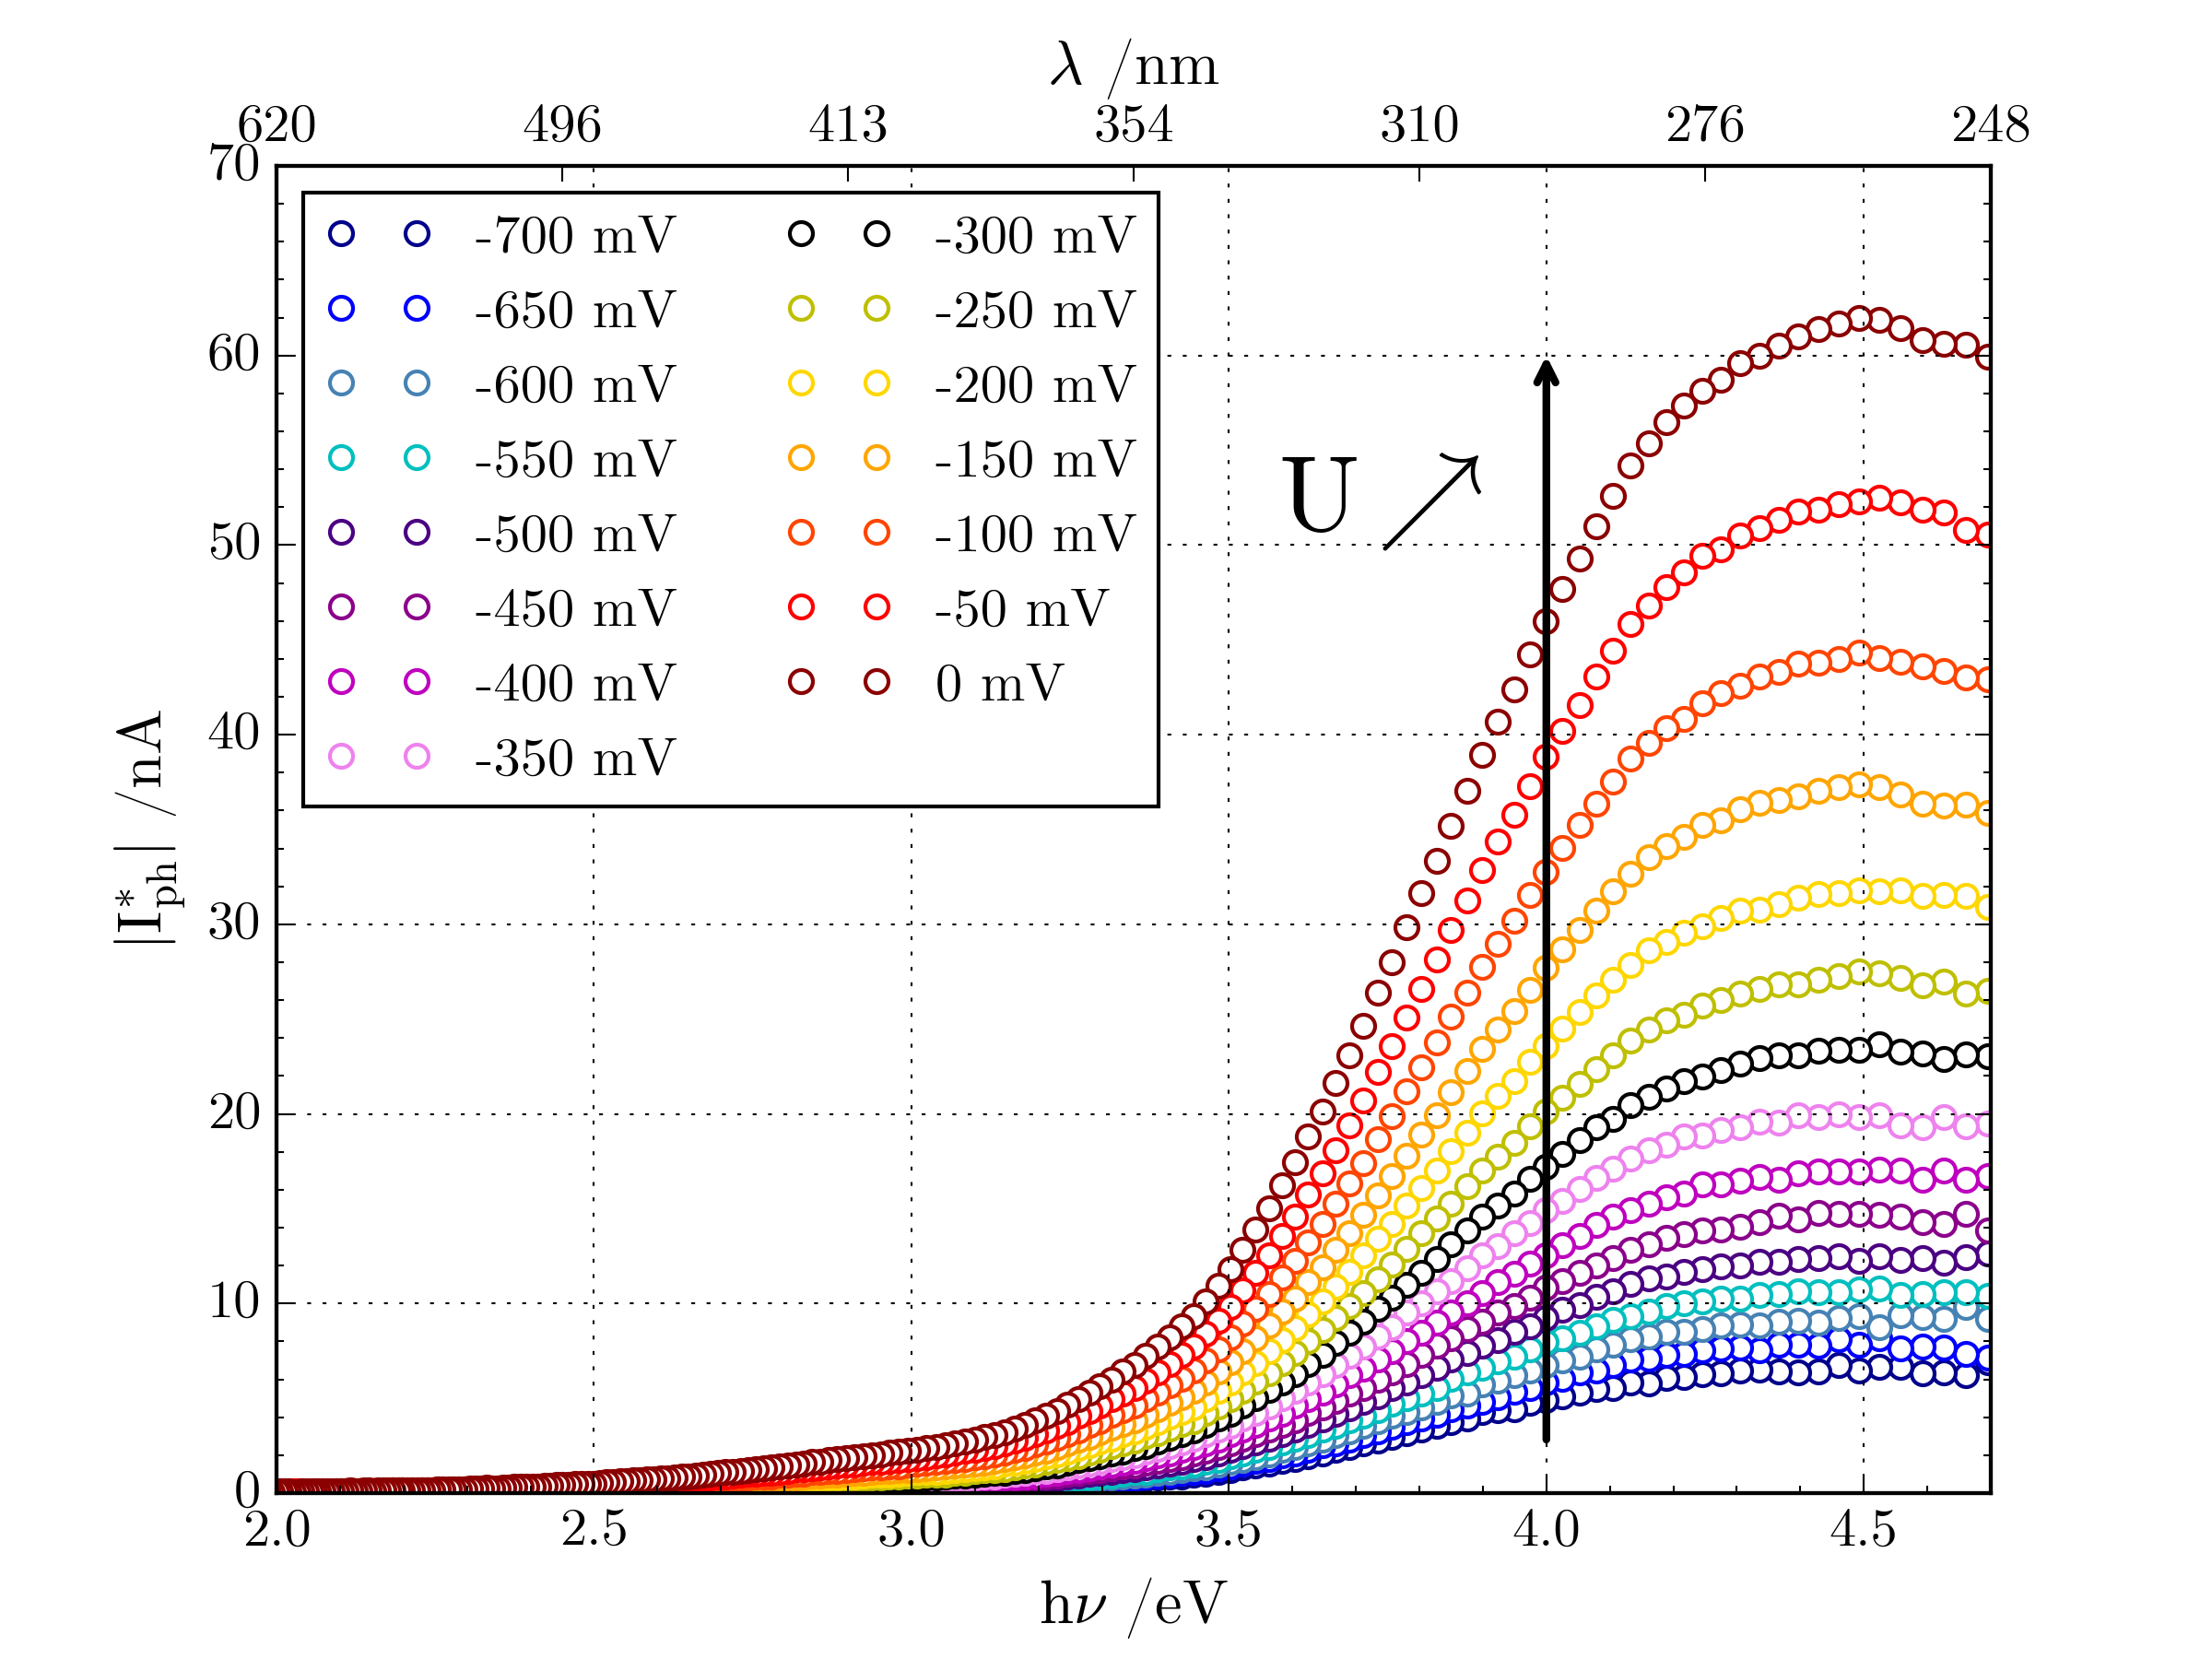
\includegraphics[width=\textwidth]{140778-PEC-X718-Iph-MA4-Polarization.png}
                \caption{}
                \label{}
            \end{subfigure}
            \begin{subfigure}[b]{0.48\textwidth}
                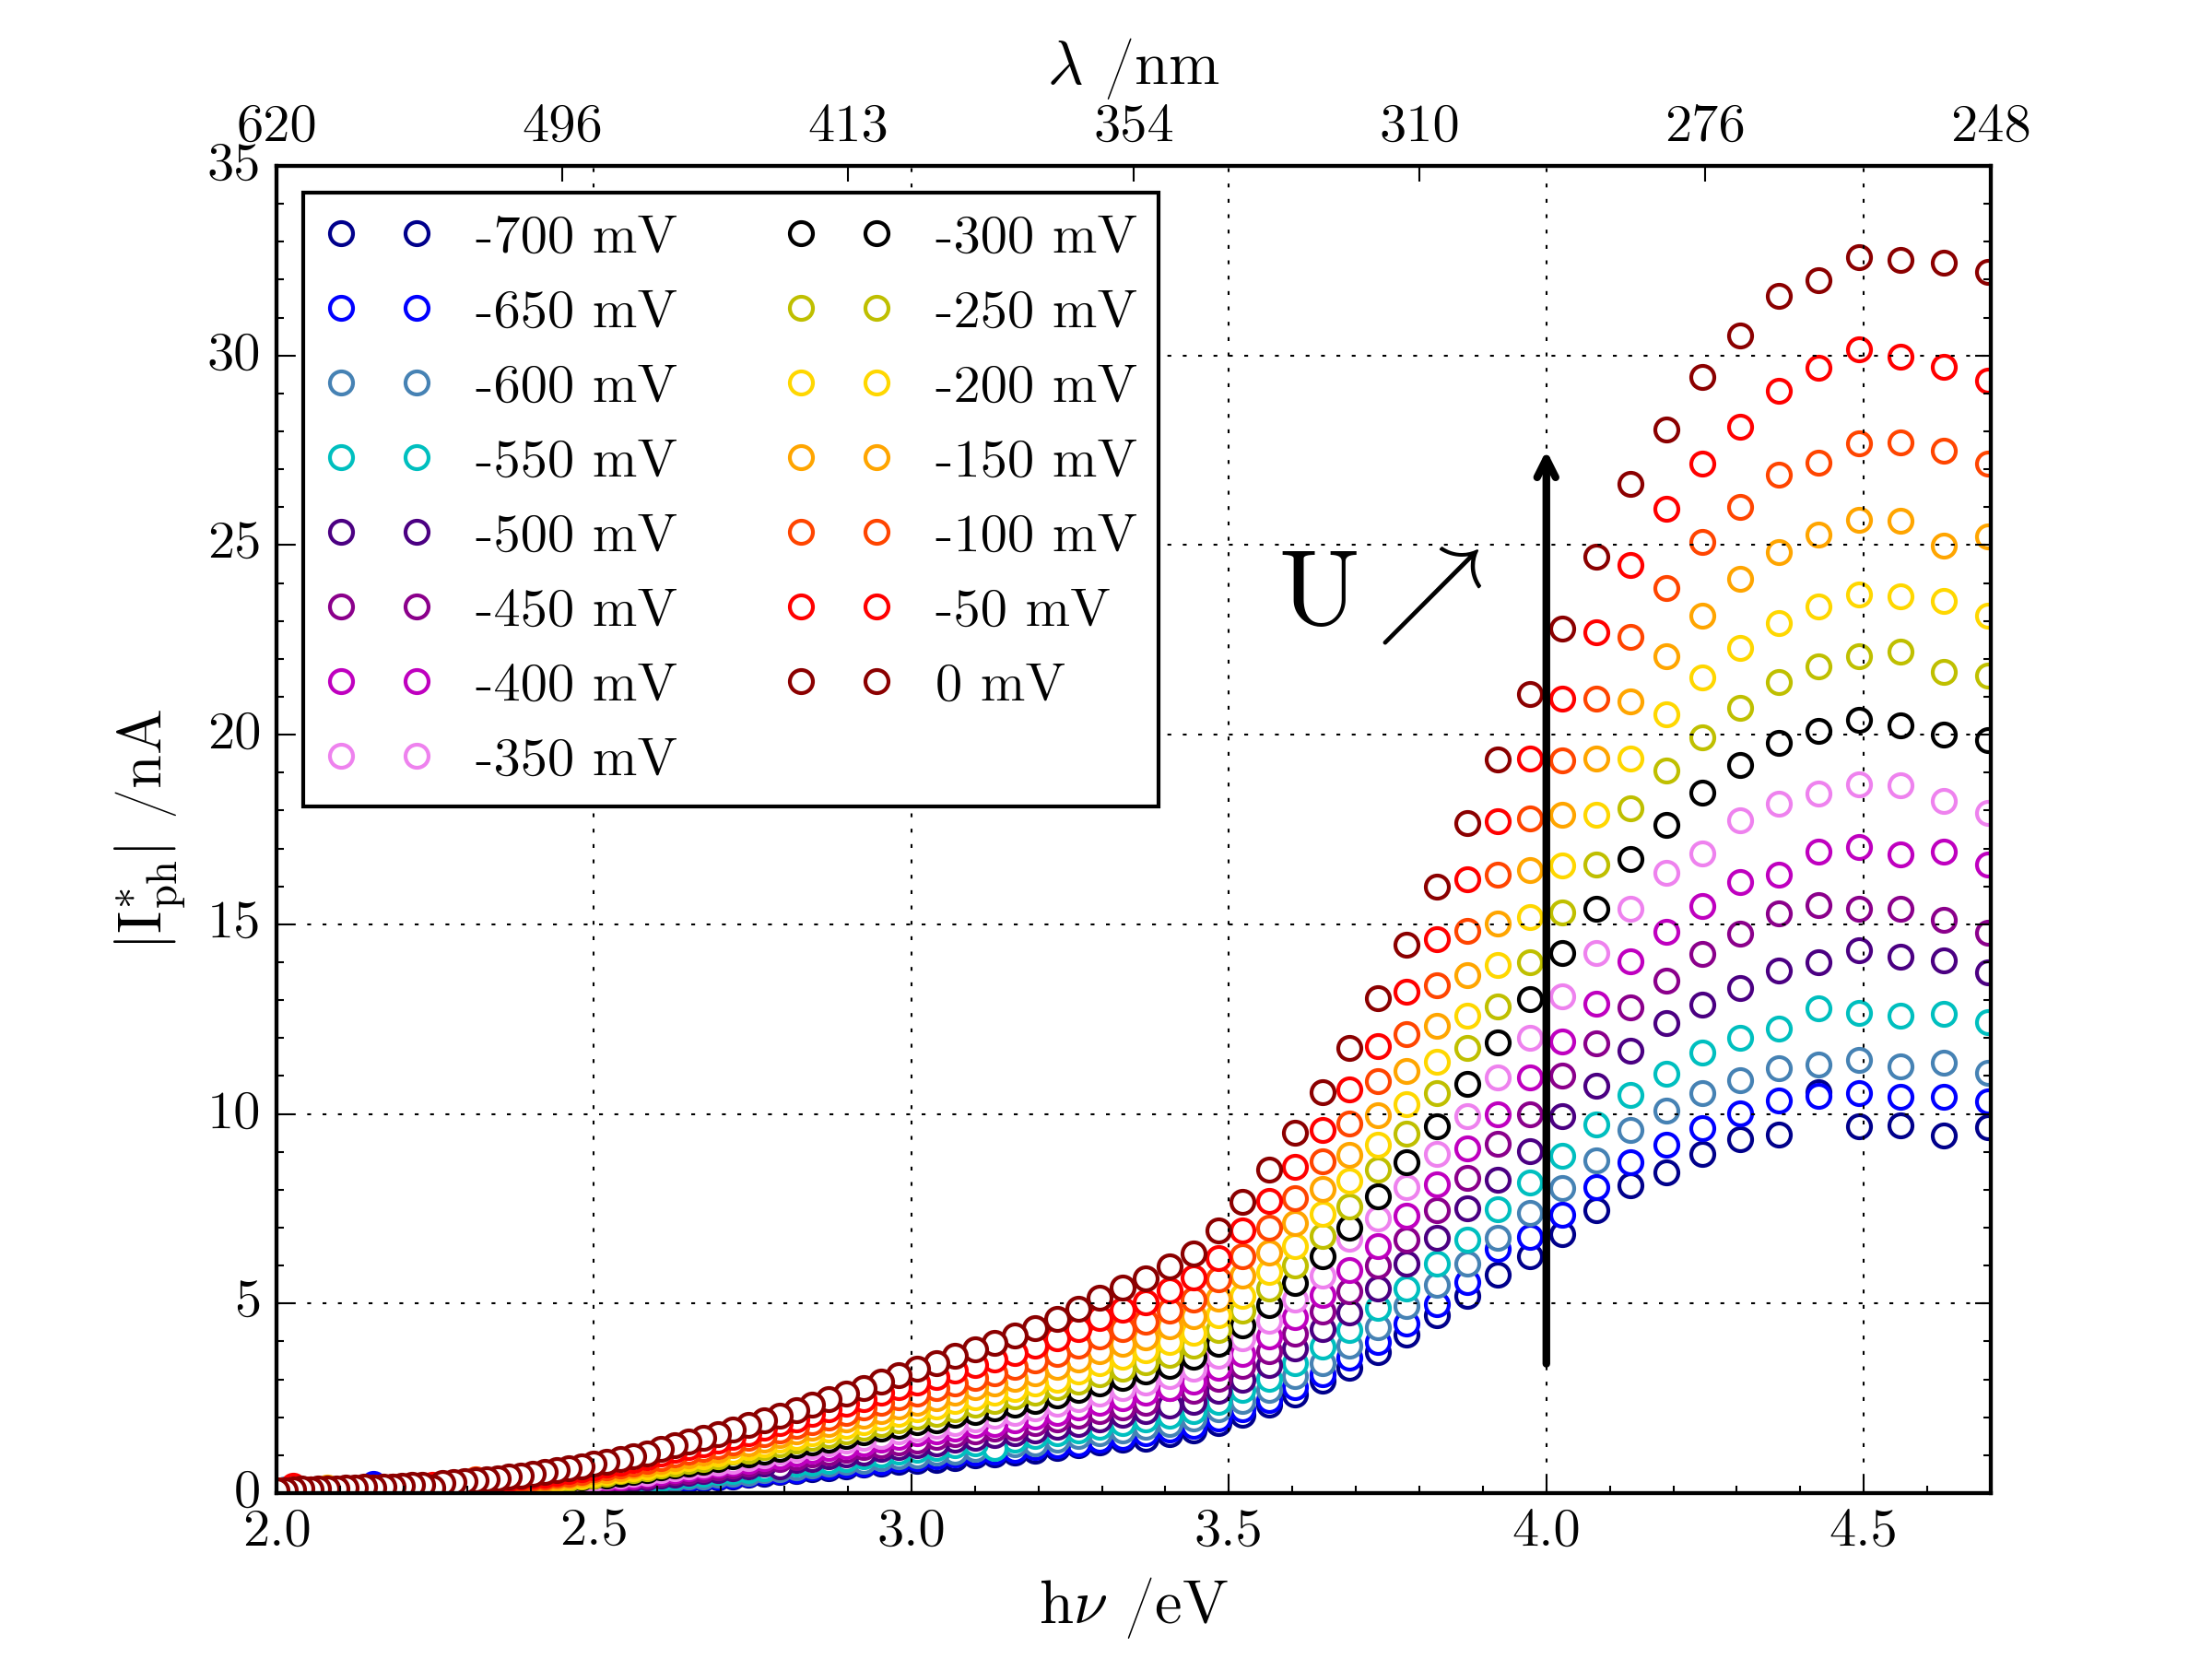
\includegraphics[width=\textwidth]{140778-PEC-X718-Iph-MA5-Polarization.png}
                \caption{}
                \label{}
            \end{subfigure}

            \caption{Spectres en énergie de photocourants mesurés à différents potentiels sur les échantillons d’Inc718
            exposés dans les différents électrolytes: a) \FeII , b) \ratio > 2, c) \ratio <2,
        d) \water.}
            \label{fig:ch4_Iph_vs_U}
        \end{figure}

        \begin{figure}[H]
            \centering
            \begin{subfigure}[b]{0.48\textwidth}
                \includegraphics[width=\textwidth]{{140778-PEC-X718-Iph-MA2-Polarization-Norm_3.97eV}.png}
                \caption{}
                \label{}
            \end{subfigure}
            \begin{subfigure}[b]{0.48\textwidth}
                \includegraphics[width=\textwidth]{{140778-PEC-X718-Iph-MA3-Polarization-Norm_3.97eV}.png}
                \caption{}
                \label{}
            \end{subfigure}
            \begin{subfigure}[b]{0.48\textwidth}
                \includegraphics[width=\textwidth]{{140778-PEC-X718-Iph-MA4-Polarization-Norm_3.97eV}.png}
                \caption{}
                \label{}
            \end{subfigure}
            \begin{subfigure}[b]{0.48\textwidth}
                \includegraphics[width=\textwidth]{{140778-PEC-X718-Iph-MA5-Polarization-Norm_3.97eV}.png}
                \caption{}
                \label{}
            \end{subfigure}
            \caption{Spectres en énergie de photocourants mesurés à différents potentiels sur les échantillons
                d’Inc718 exposés dans les différents électrolytes: a) \FeII , b) \ratio > 2, c) \ratio <2,
        d) \water. Pour chaque spectre, les photocourants ont été normalisés à 1 pour une
        énergie de 4~eV.}
            \label{fig:ch4_Iph_vs_U_Normalized}
        \end{figure}

    Il est possible de s’en convaincre encore davantage en sommant les spectres en énergie mesurés à différents
    potentiels, c’est-à-dire en sommant à chaque énergie les photocourants complexes mesurés à chaque potentiel, de
    manière à obtenir un spectre "virtuel", ou "spectre somme" qui sera à son tour ajusté numériquement. Si
    l’ensemble des spectres en énergie mesurés à différents potentiels peuvent être décrits par les mêmes
    contributions déterminées au potentiel d’abandon, l’ajustement numérique du spectre "somme" doit fournir ces
    mêmes contributions et celles-là seulement. 

    La procédure décrite ci-dessus a effectivement été appliquée aux spectres en énergie de photocourants mesurés à
    différents potentiels, pour chaque échantillon. Par exemple, pour l’échantillon formé en eau pure (spectres de la figure
    \ref{fig:ch4_Iph_vs_U}d) , le tableau \ref{tab:ch4_Eg_comp_OCV_sum} compare les valeurs de gaps déduites de l’ajustement du spectre "somme" avec celles tirées de
    l’ajustement du spectre mesuré au potentiel d’abandon. Les deux ajustements fournissent le même nombre de gaps, ainsi
    que les mêmes valeurs de largeurs de bande interdite, à l’intervalle de confiance près.

    
    \begin{table}[H]
        \centering
        \begin{tabular}{p{0.1\textwidth}|%
                        p{0.2\textwidth}%
                        p{0.2\textwidth}%
                        }
            \toprule
            & \water\ -- OCV & \water\ -- Somme\\ \midrule
            \rowcolor{lightgray}$E_{g,1}$ /eV & 2.08 $\pm$ 0.08 & 2.10 $\pm$ 0.03 \\\hline
           $E_{g,2}$ /eV & 3.30 $\pm$ 0.02 & 3.28 $\pm$ 0.02 \\\hline
            \rowcolor{lightgray}$E_{g,3}$ /eV & 3.90 $\pm$ 0.04 & 3.89 $\pm$ 0.03 \\\hline
            $E_{g,4}$ /eV & 4.2 $\pm$ 0.2 & 4.30 $\pm$ 0.09 \\
            \bottomrule
        \end{tabular}
        \caption{Valeurs des largeurs de bande interdite déduites de l’ajustement numérique du spectre en énergie de
        photocourants mesuré au potentiel d’abandon et de celui du spectre "somme", pour l’échantillon Inc718 oxydé en
    eau pure.}
        \label{tab:ch4_Eg_comp_OCV_sum}
    \end{table}

    \paragraph{Photovoltammogrammes}\label{par:photovoltammogram}
    \mbox{}\\
    Nous avons montré au paragraphe précédent que pour chaque échantillon, les spectres en énergie de photocourants
    normalisés mesurés aux différents potentiels appliqués se superposent quasi-parfaitement (figure \ref{fig:ch4_Iph_vs_U_Normalized}). Il est donc
    possible d’étudier l’évolution des photocourants avec le potentiel en se limitant à l’analyse des photovoltammogrammes
    pour une seule énergie, par exemple 4~eV, comme illustré dans la figure \ref{fig:ch4_Iph_vs_U}, qui rassemble les photovoltammogrammes à 
    4~eV extraits des données de la figure \ref{fig:ch4_Iph_vs_U}.

    Le photocourant des échantillons oxydés dans les électrolytes \water\ et \ratio >2 augmente peu et à peu près
    linéairement avec le potentiel. L’allure du photovoltammogramme est proche de celle de la branche anodique d’un
    photovoltammogramme en "V" typique d’un matériau  isolant, ou très peu dopé (chapitre \ref{chap:ch1_bib}, figure
    \ref{fig:loucif_application}). En revanche, le
    photocourant des échantillons formés dans les électrolytes \FeII et \ratio <2 augmente plus rapidement
    avec le potentiel et de manière non linéaire, suggérant un dopage plus important. La normalisation à 1 pour un potentiel
    appliqué de -300~mV illustre que le photocourant des échantillons exposés dans les électrolytes \FeII et
    \ratio <2 présente une évolution similaire de photocourant comme illustré en figure \ref{fig:ch4_photovolt_Inc718_Normalized}.
    L’amplitude de
    photocourant plus importante dans le cas de l’électrolyte \FeII\ suggère un dopage plus important.

    Ainsi, il semble que les électrolytes \FeII\ et \ratio <2 favoriseraient la formation de couches
    d’oxyde plus dopées, et les électrolytes \ratio >2 et \water\ des couches d’oxyde à caractère plus
    isolant. La présence de cations de fer seuls dans l’électrolyte favoriserait une couche d’oxyde plus dopée et
    donc plus conductrice, ce qui paraît en accord avec les mesures de courant de couplage présentées plus haut qui
    indiquent que le contact galvanique a un effet important dans cet électrolyte. 


    \begin{figure}[H]
        \centering
        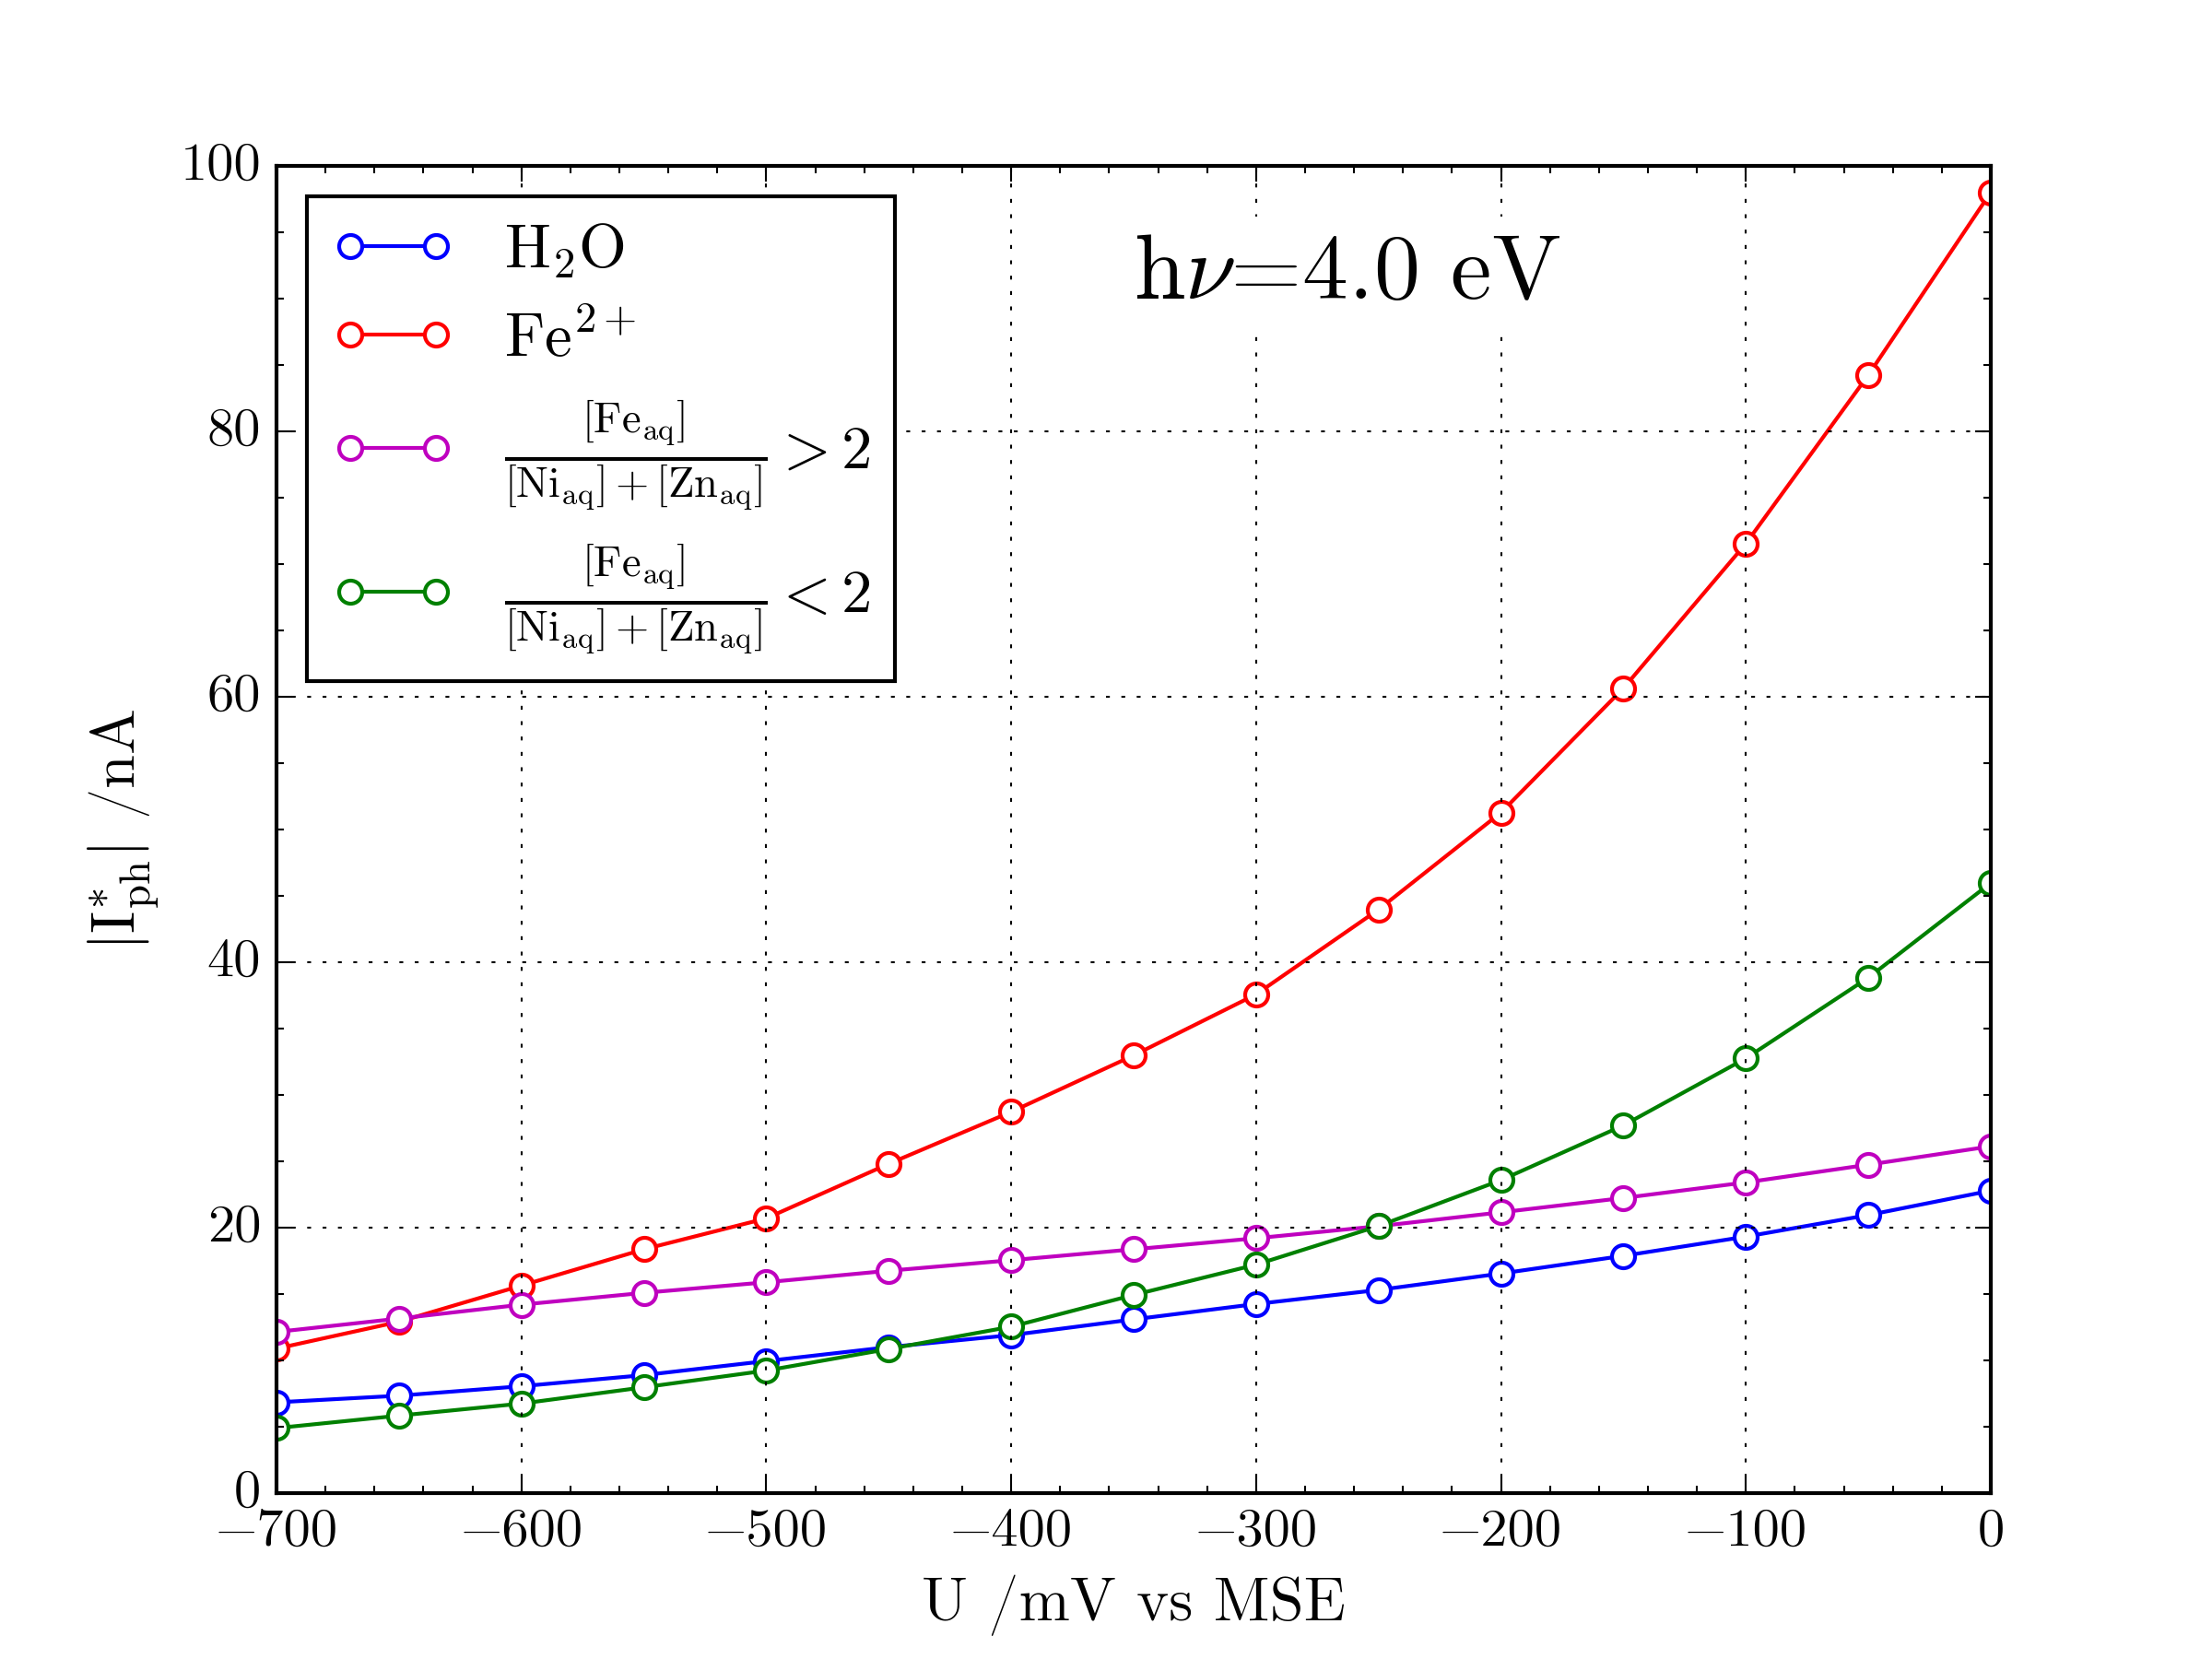
\includegraphics[width=\figwidth]{140778-PEC-X718-Iph_vs_hv-all.png}
        \caption{Photovoltammogrammes à 4~eV des échantillons d’Inc718 oxydés dans les quatre électrolytes sélectionnés.}
        \label{fig:ch4_photovolt_Inc718}
    \end{figure}

    \begin{figure}[H]
        \centering
        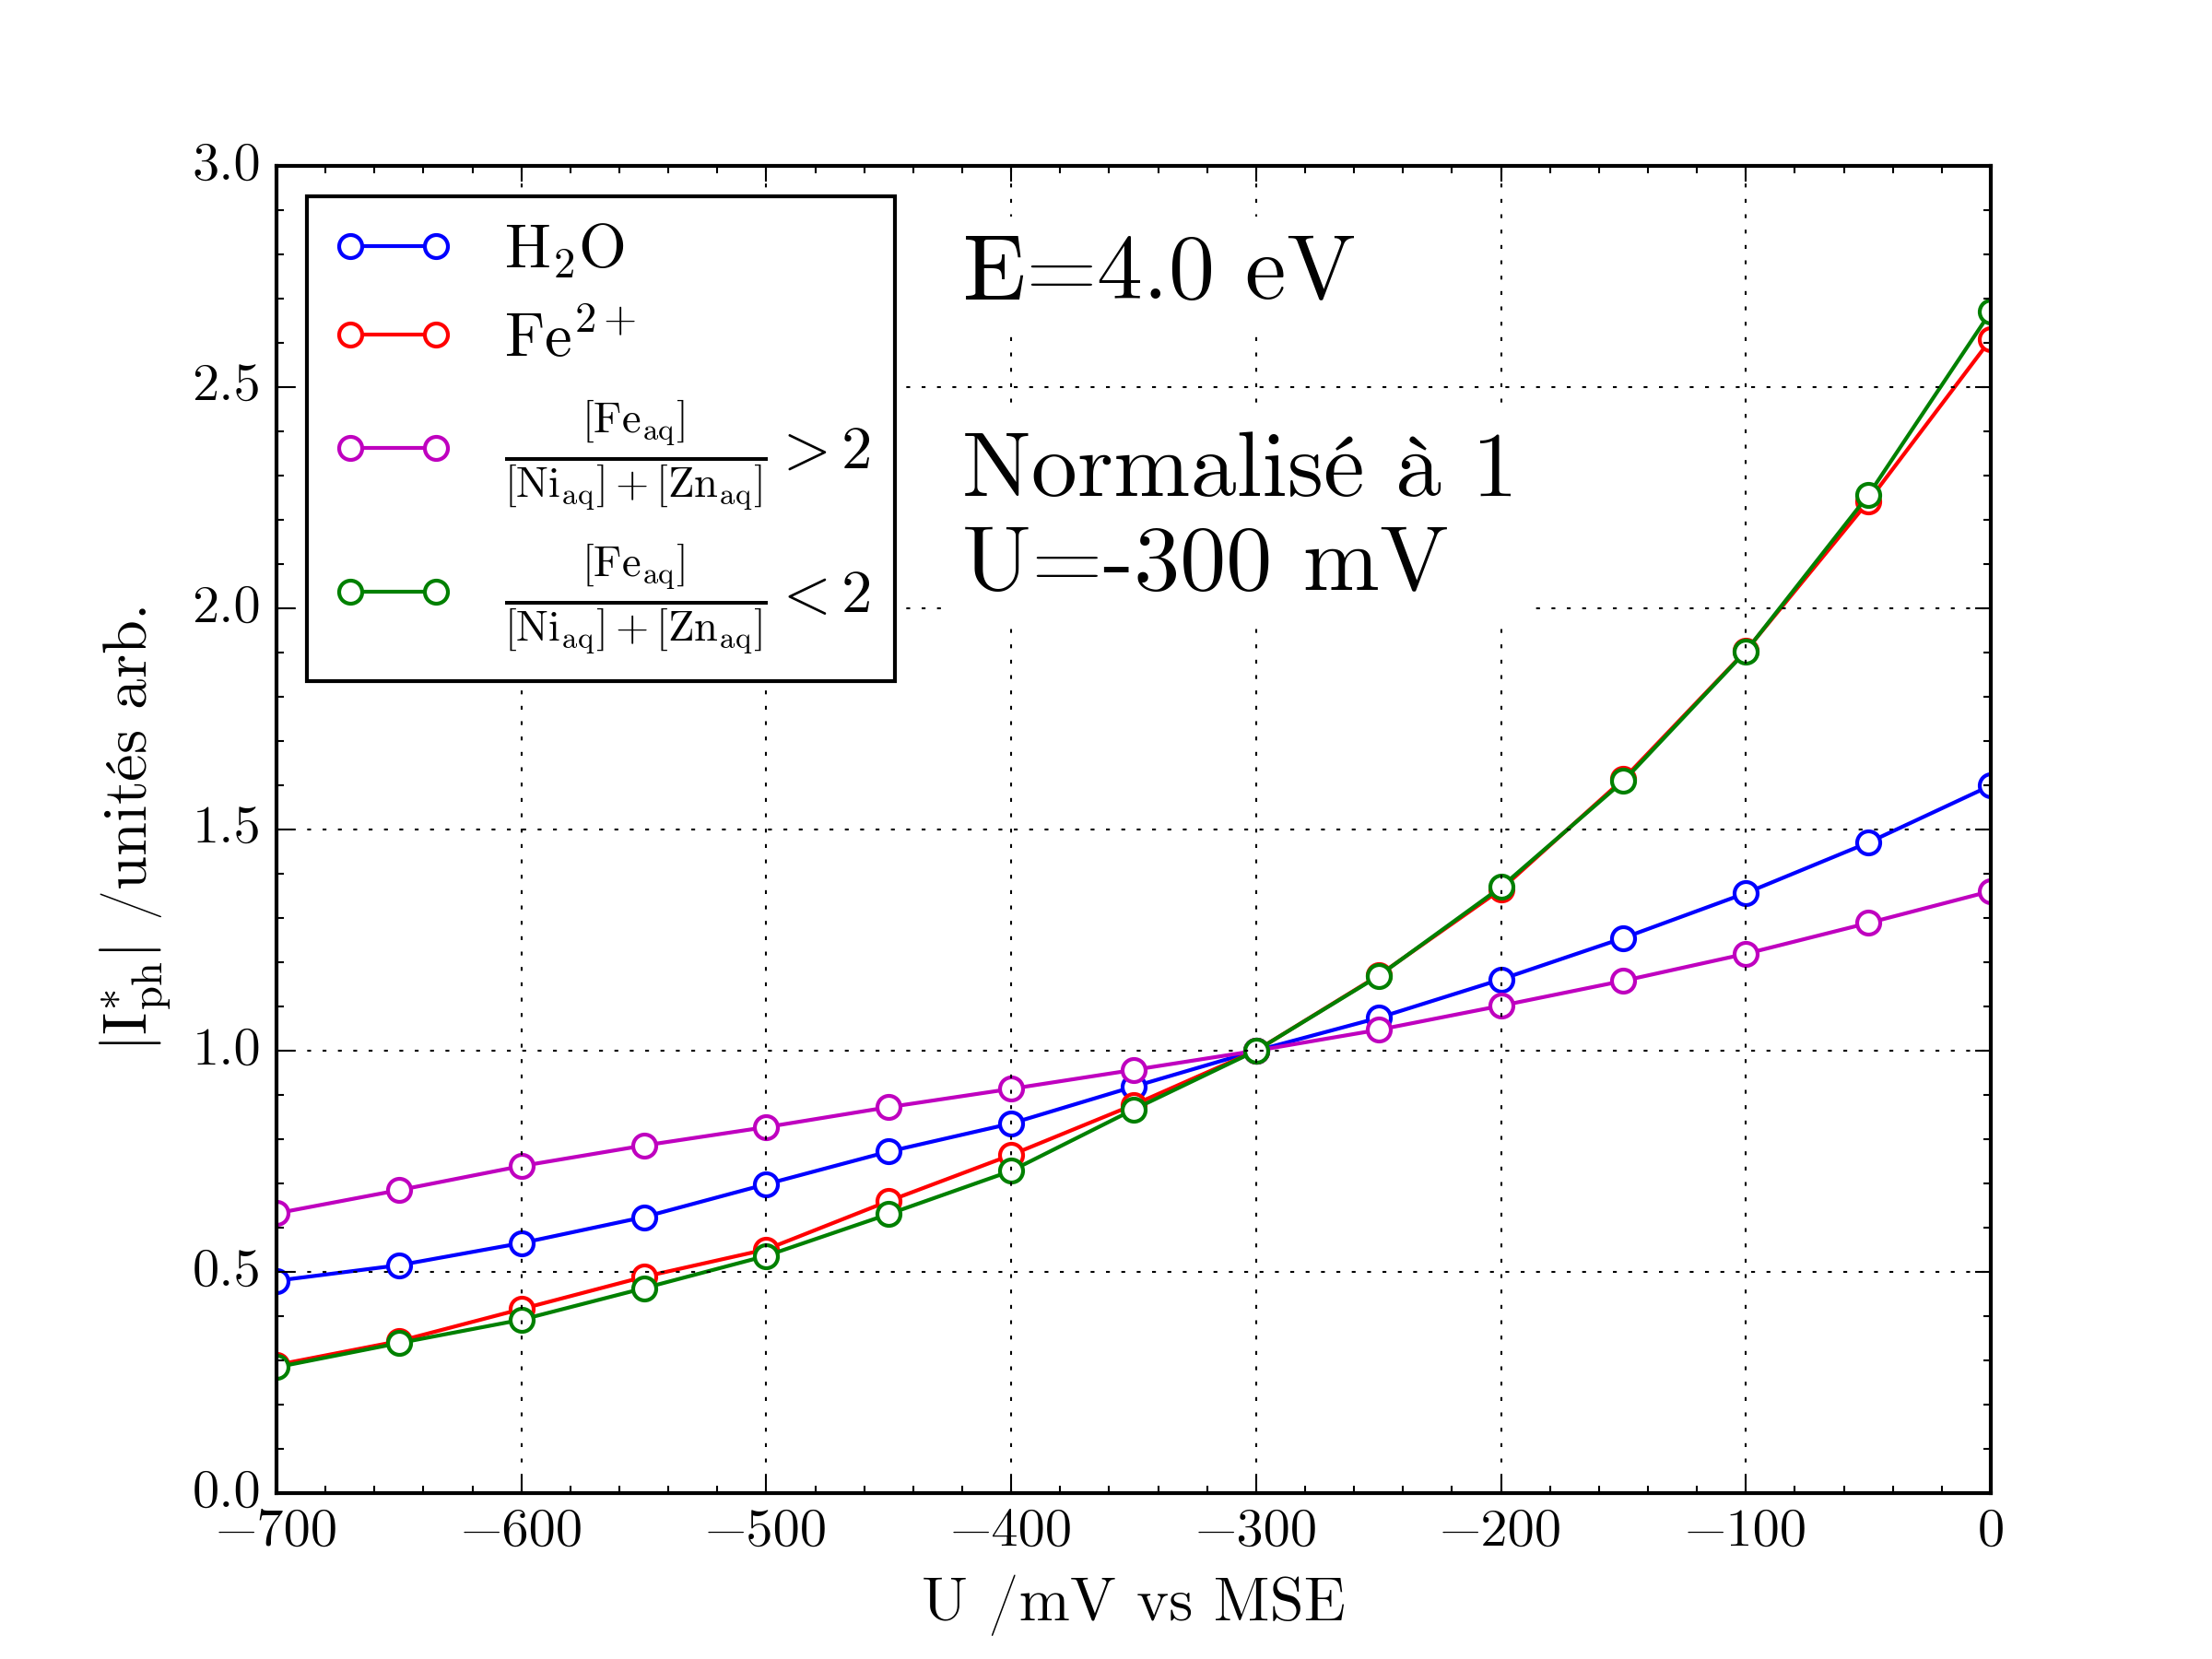
\includegraphics[width=\figwidth]{140778-PEC-X718-Iph_vs_hv-all-Norm_-300mV.png}
        \caption{Photovoltammogrammes à 4~eV des échantillons d’Inc718 oxydés dans les quatre électrolytes sélectionnés
        de la figure \ref{fig:ch4_photovolt_Inc718} normalisé à 1 pour un potentiel de -300~mV.}
        \label{fig:ch4_photovolt_Inc718_Normalized}
    \end{figure}




    \subsubsection{Echantillon de Zy2}\label{subsubsec:Zy2_samples}


    La figure \ref{fig:ch4_Iph_OCV_Zy2} présente les spectres en énergie de photocourants mesurés au potentiel d’abandon sur le côté
    intérieur des coupons rectangulaires ainsi que les courbes obtenues par ajustement numérique des points
    expérimentaux. Etant donné que l’amplitude des photocourants est très différente d’un électrolyte de formation des
    couches d’oxydation à l’autre, les spectres de la figure \ref{fig:ch4_Iph_OCV_Zy2} ont été retracés en figure \ref{fig:ch4_Iph_OCV_Zy2_Normalized} en normalisant
    l’amplitude des photocourants à 1 pour une énergie de 3.9~eV, dans le but de faciliter l’évaluation de l’effet
    de électrolyte sur les couches d'oxydation. Signalons par ailleurs que les importantes épaisseurs de zircone obtenues dans les
    électrolytes \FeII, \ratio >2 et \ratio <2 ont eu pour conséquence un trop faible
    rapport signal/bruit pour les mesures faites au-delà de 4.5~eV (c’est-à dire pour les énergies auxquelles le flux de
    photons délivré par la source Xenon est très faible), mesures qui ne sont donc pas présentées. 
    
    Dans le cas de l’échantillon oxydé dans l’électrolyte ne contenant que des cations de fer, le spectre en énergie de
    photocourants apparaît peu différent de celui oxydé dans l’eau pure. En revanche, on note que lorsque les
    concentrations en cations nickel et zinc augmentent par rapport à la concentration en cations de fer, l’amplitude
    des photocourants, pour des énergies inférieures à 3.5~eV, semble être exacerbée, suggérant que la présence de ces
    cations nickel et/ou zinc favorise la formation d’une phase semiconductrice dont la largeur de bande interdite est
    inférieure à 3.5~eV.

    \begin{figure}[H]
        \centering
        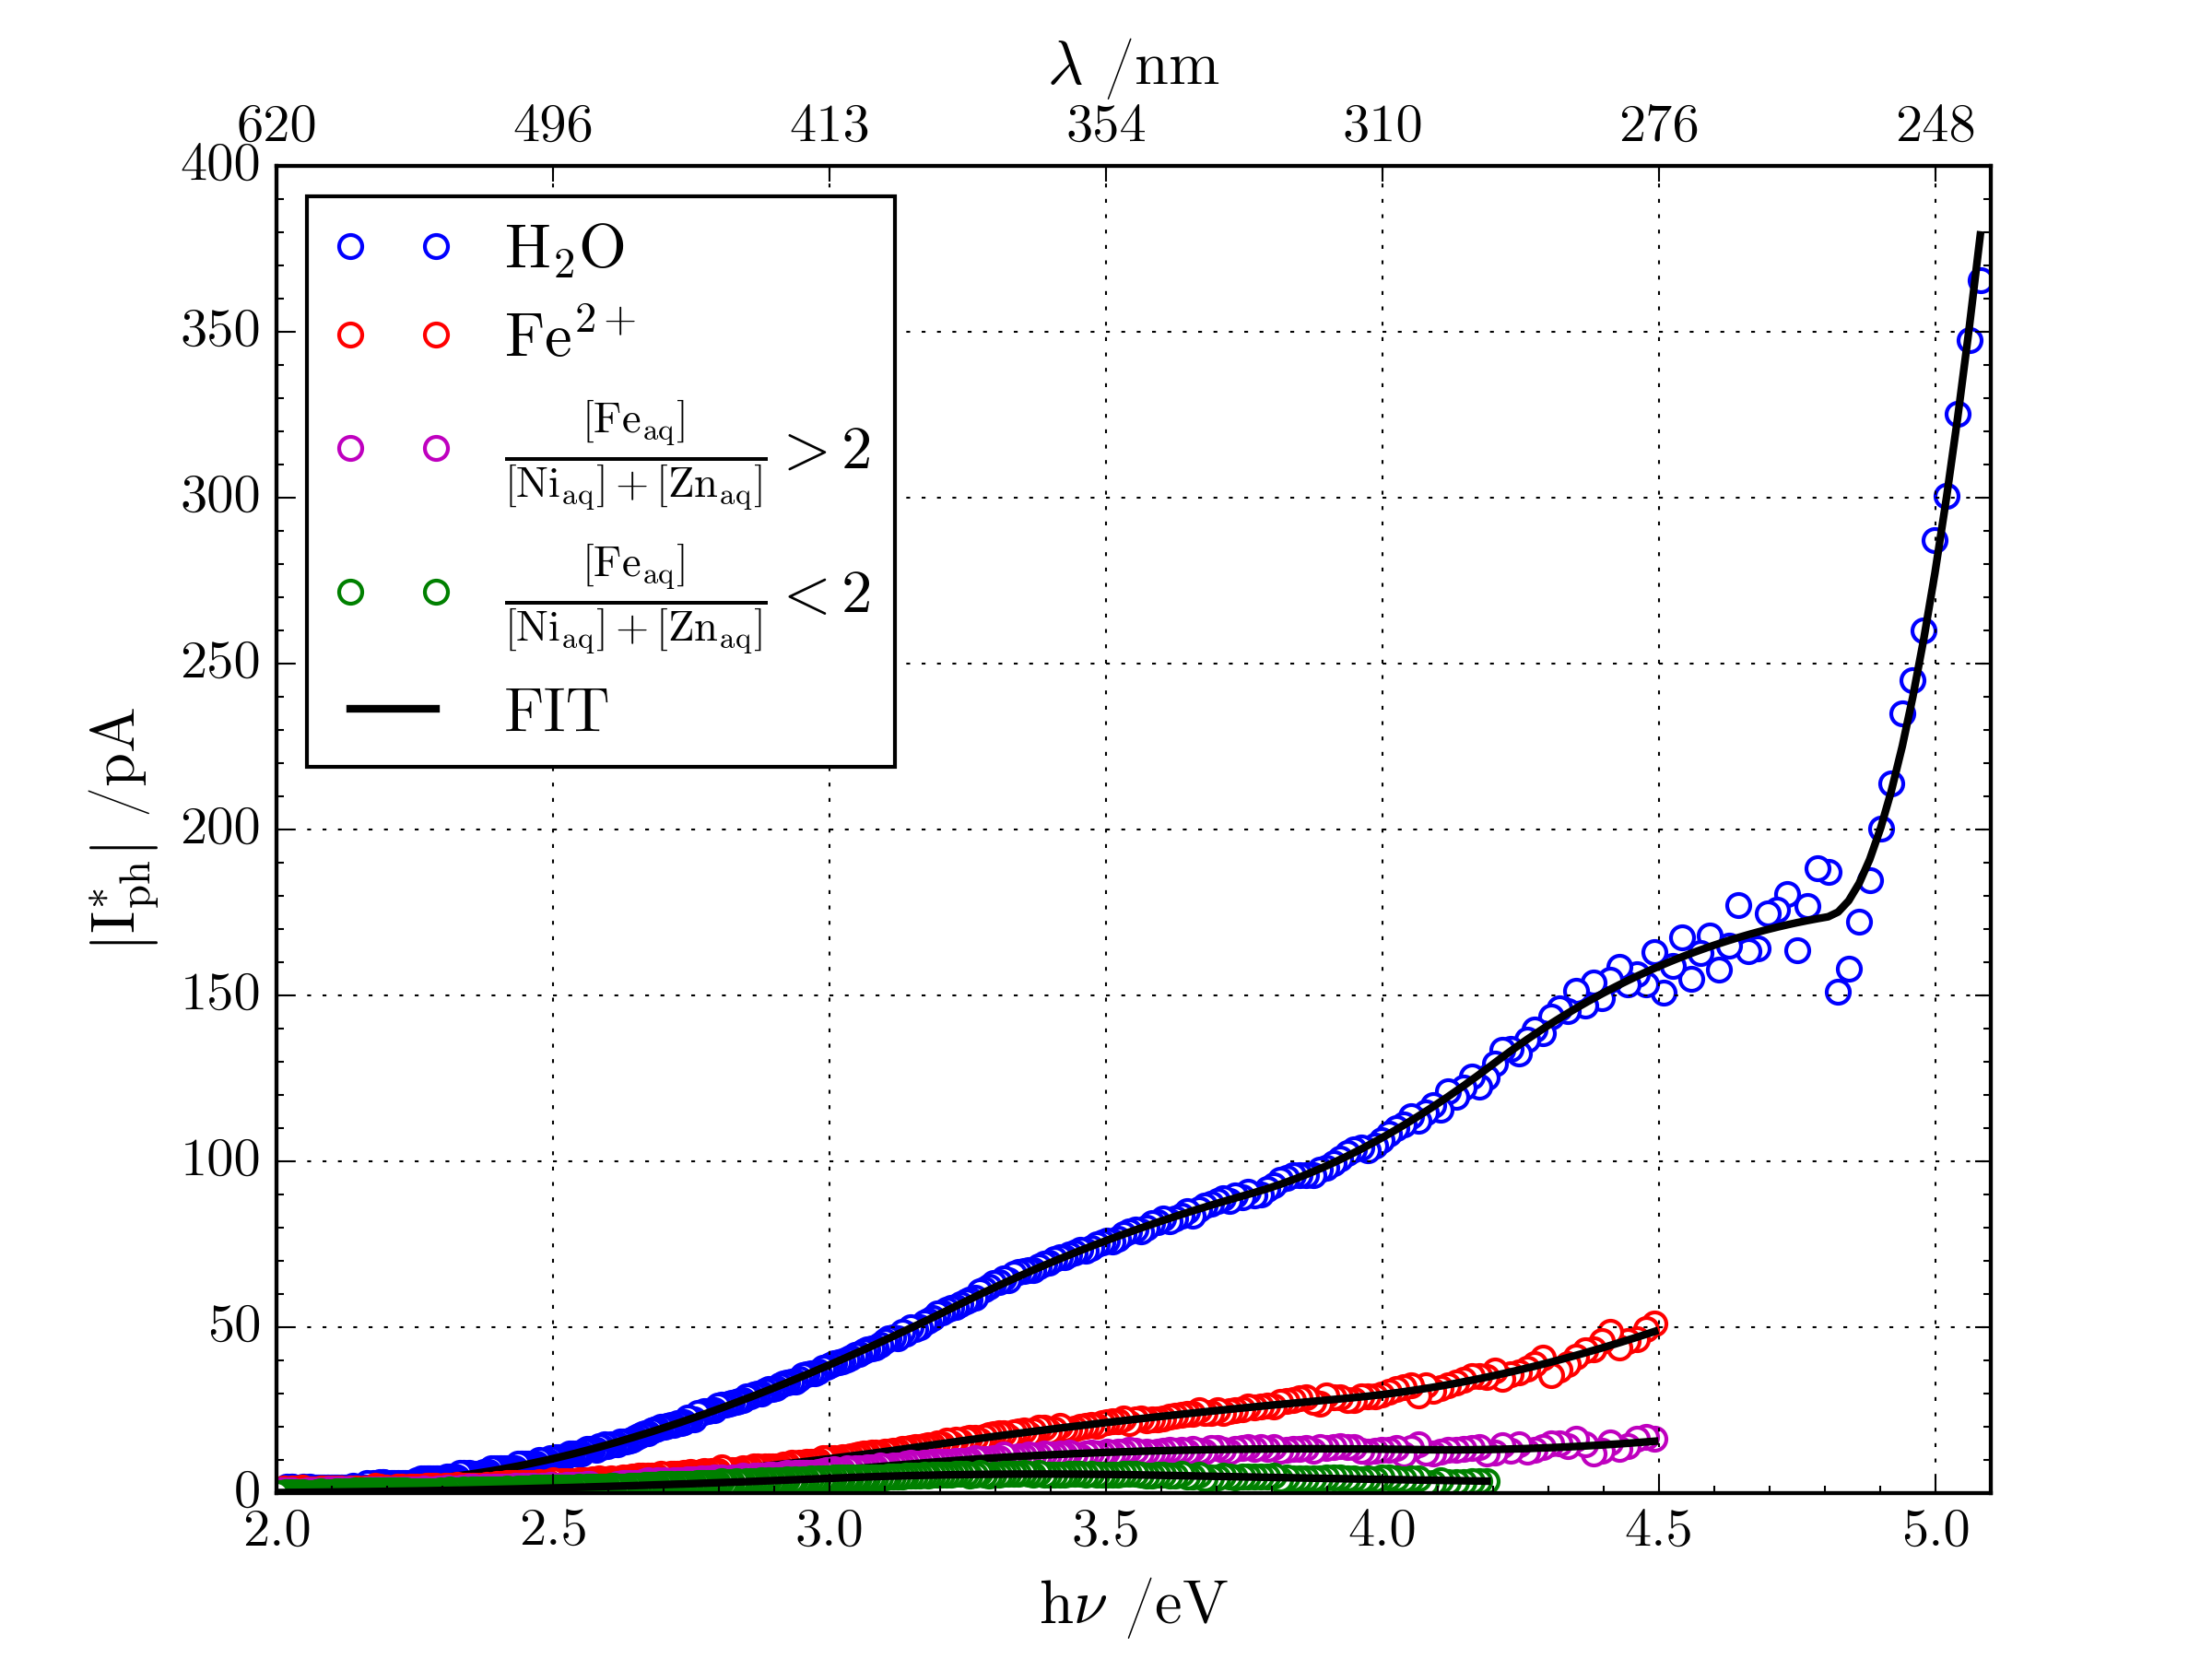
\includegraphics[width=\figwidth]{140778-PEC-Fit-Zy2-Iph.png}
        \caption{Spectres en énergie de photocourants mesurés sur le côté intérieur des coupons rectangulaires de Zy2
            (couplés) exposés à \SI{280}{\degreeCelsius} dans les quatre électrolytes sélectionnés. "FIT" indique les courbes obtenues par
    ajustement numérique.}
        \label{fig:ch4_Iph_OCV_Zy2}
    \end{figure}

    \begin{figure}[H]
        \centering
        \includegraphics[width=\figwidth]{{140778-PEC-Fit-Zy2-Iph-Norm_3.87eV}.png}
        \caption{Spectres en énergie de photocourants de la figure \ref{fig:ch4_Iph_OCV_Zy2} normalisés à 
            1 pour une énergie de 3.9 eV. "FIT"
        indique les courbes obtenues par ajustement numérique.}
        \label{fig:ch4_Iph_OCV_Zy2_Normalized}
    \end{figure}


    Les valeurs de gaps, et les incertitudes correspondantes, déduites des ajustements numériques des spectres de la
    figure \ref{fig:ch4_Iph_OCV_Zy2}, pour les échantillons oxydés dans les quatre électrolytes retenus sont listées
    dans le tableau \ref{tab:ch4_band_gaps_fit_Zy2}, et
    également représentées graphiquement en figure \ref{fig:ch4_Eg_Zy2_graph}.

    Pour l’échantillon formé en milieu \water\, le gap de la phase d’oxyde majoritaire, c’est-à-dire la zircone
    monoclinique, est bien détectée, avec une largeur de bande interdite de 4.81~eV. Comme dans le cas des échantillons
    d’Inc718, une valeur de gap d’environ 4.2~eV est obtenue, attribuée à un spinelle de type $Ni_{1-x}Fe_xCr_2O_4$. 
    
    Pour les échantillons formés dans les autres électrolytes, le niveau de bruit élevé n’a pas permis de signer la
    présence de la zircone monoclinique, mais il serait très surprenant qu’elle ne soit pas présente dans la couche.
    Nous proposons d’assigner la largeur de bande interdite allant de 3.7 à 3.9~eV à l’oxyde d’étain $SnO_2$ étant donné
    que l’alliage Zy2 contient 1.32\% d’étain. 
    
    Les gaps allant de 3.01 à 3.24~eV signent certainement de la chromine et/ou un spinelle de type $AB_2O_4$ telle que
    $FeCr_2O_4$ \citep{DiQuarto2000}, ceux allant de 1.7 à 1.8~eV correspondant à de l’hématite (plus ou moins hydratée) \citep{Benaboud2007,Wouters2004,Srisrual2009}. 
    Les gaps
    intermédiaires (2.2 à 2.49~eV) sont raisonnablement attribuables à des solutions solides de type $(Fe, Cr)_2O_3$
    \citep{Srisrual2009}.
    
    Pour conclure ce paragraphe, notons qu’à la différence de ce qui a été observé pour les échantillons d’Inc718, la
    présence d’impuretés dans l’électrolyte d’oxydation ne semble pas favoriser l’apparition de composé en plus dans la
    couche par rapport à celles détectées sur la couche formée en \water\ pure.


     \begin{table}[H]
         \begin{footnotesize}
        \centering
        \begin{tabular}{p{0.05\textwidth}|%
                        p{0.11\textwidth}%
                        p{0.14\textwidth}%
                        p{0.18\textwidth}%
                        p{0.15\textwidth}%
                        p{0.18\textwidth}%
                        }
            \toprule
            & \water & \FeII & $\frac{[Fe_{aq}]}{[Ni_{aq}]+[Zn_{aq}]}$>2 & $\frac{[Fe_{aq}]}{[Ni_{aq}]+[Zn_{aq}]}$<2 & Attributions \\ \midrule
            \rowcolor{lightgray}$E_{g,1}$ & 1.8 $\pm$ 0.2 & 1.7 $\pm$ 0.2 & 1.71 $\pm$ 0.06 & 1.8 $\pm$ 0.1 & $Fe_2O_3$
            \citep{Benaboud2007,Wouters2004,Srisrual2009}\\\hline 
            $E_{g,2}$ & 2.3 $\pm$ 0.2 & 2.49 $\pm$ 0.08 & 2.47 $\pm$ 0.09 & 2.2 $\pm$ 0.3 & $(Fe, Cr)_2O_3$
            \citep{Benaboud2007,Wouters2004,Srisrual2009} \\ \hline
             \rowcolor{lightgray}$E_{g,3}$& 3.24 $\pm$ 0.09 & 3.2 $\pm$ 0.2 & 3.13 $\pm$ 0.05 & 3.01 $\pm$ 0.04 & $FeCr_2O_4$ \citep{DiQuarto2000} \\ 
            \rowcolor{lightgray}&  &  &  &  & $Cr_2O_3$
            \citep{Benaboud2007,Wouters2004,Srisrual2009},
            \citep{Wouters2008,Marchetti2010,Galerie2011,Henry2000}\\\hline
            $E_{g,4}$ & 3.8 $\pm$ 0.1 & 3.9 $\pm$ 0.2 & & 3.70 $\pm$ 0.2 & $SnO_2$ \citep{Wang2007} \\ \hline
            \rowcolor{lightgray}$E_{g,5}$ & 4.2 $\pm$ 0.2 &  & 4.1 $\pm$ 0.2 & & $Ni_{1-x}Fe_xCr_2O_4$
            \citep{Marchetti2010}\\ \hline
            $E_{g,6}$ & 4.81 $\pm$ 0.07 & & & & $ZrO_2$ \citep{Benaboud2007}\\ 
            \bottomrule
        \end{tabular}
        \caption{Valeurs de largeur de bande interdite ($E_{g,i}$ en eV) déduites des ajustements numériques des spectres en
        énergie de photocourants de la 
        figure \ref{fig:ch4_Iph_OCV_Zy2} pour
    les couches formées dans les quatre électrolytes considérés.}
        \label{tab:ch4_band_gaps_fit_Zy2}
    \end{footnotesize}
    \end{table}


    \begin{figure}[H]
        \centering
        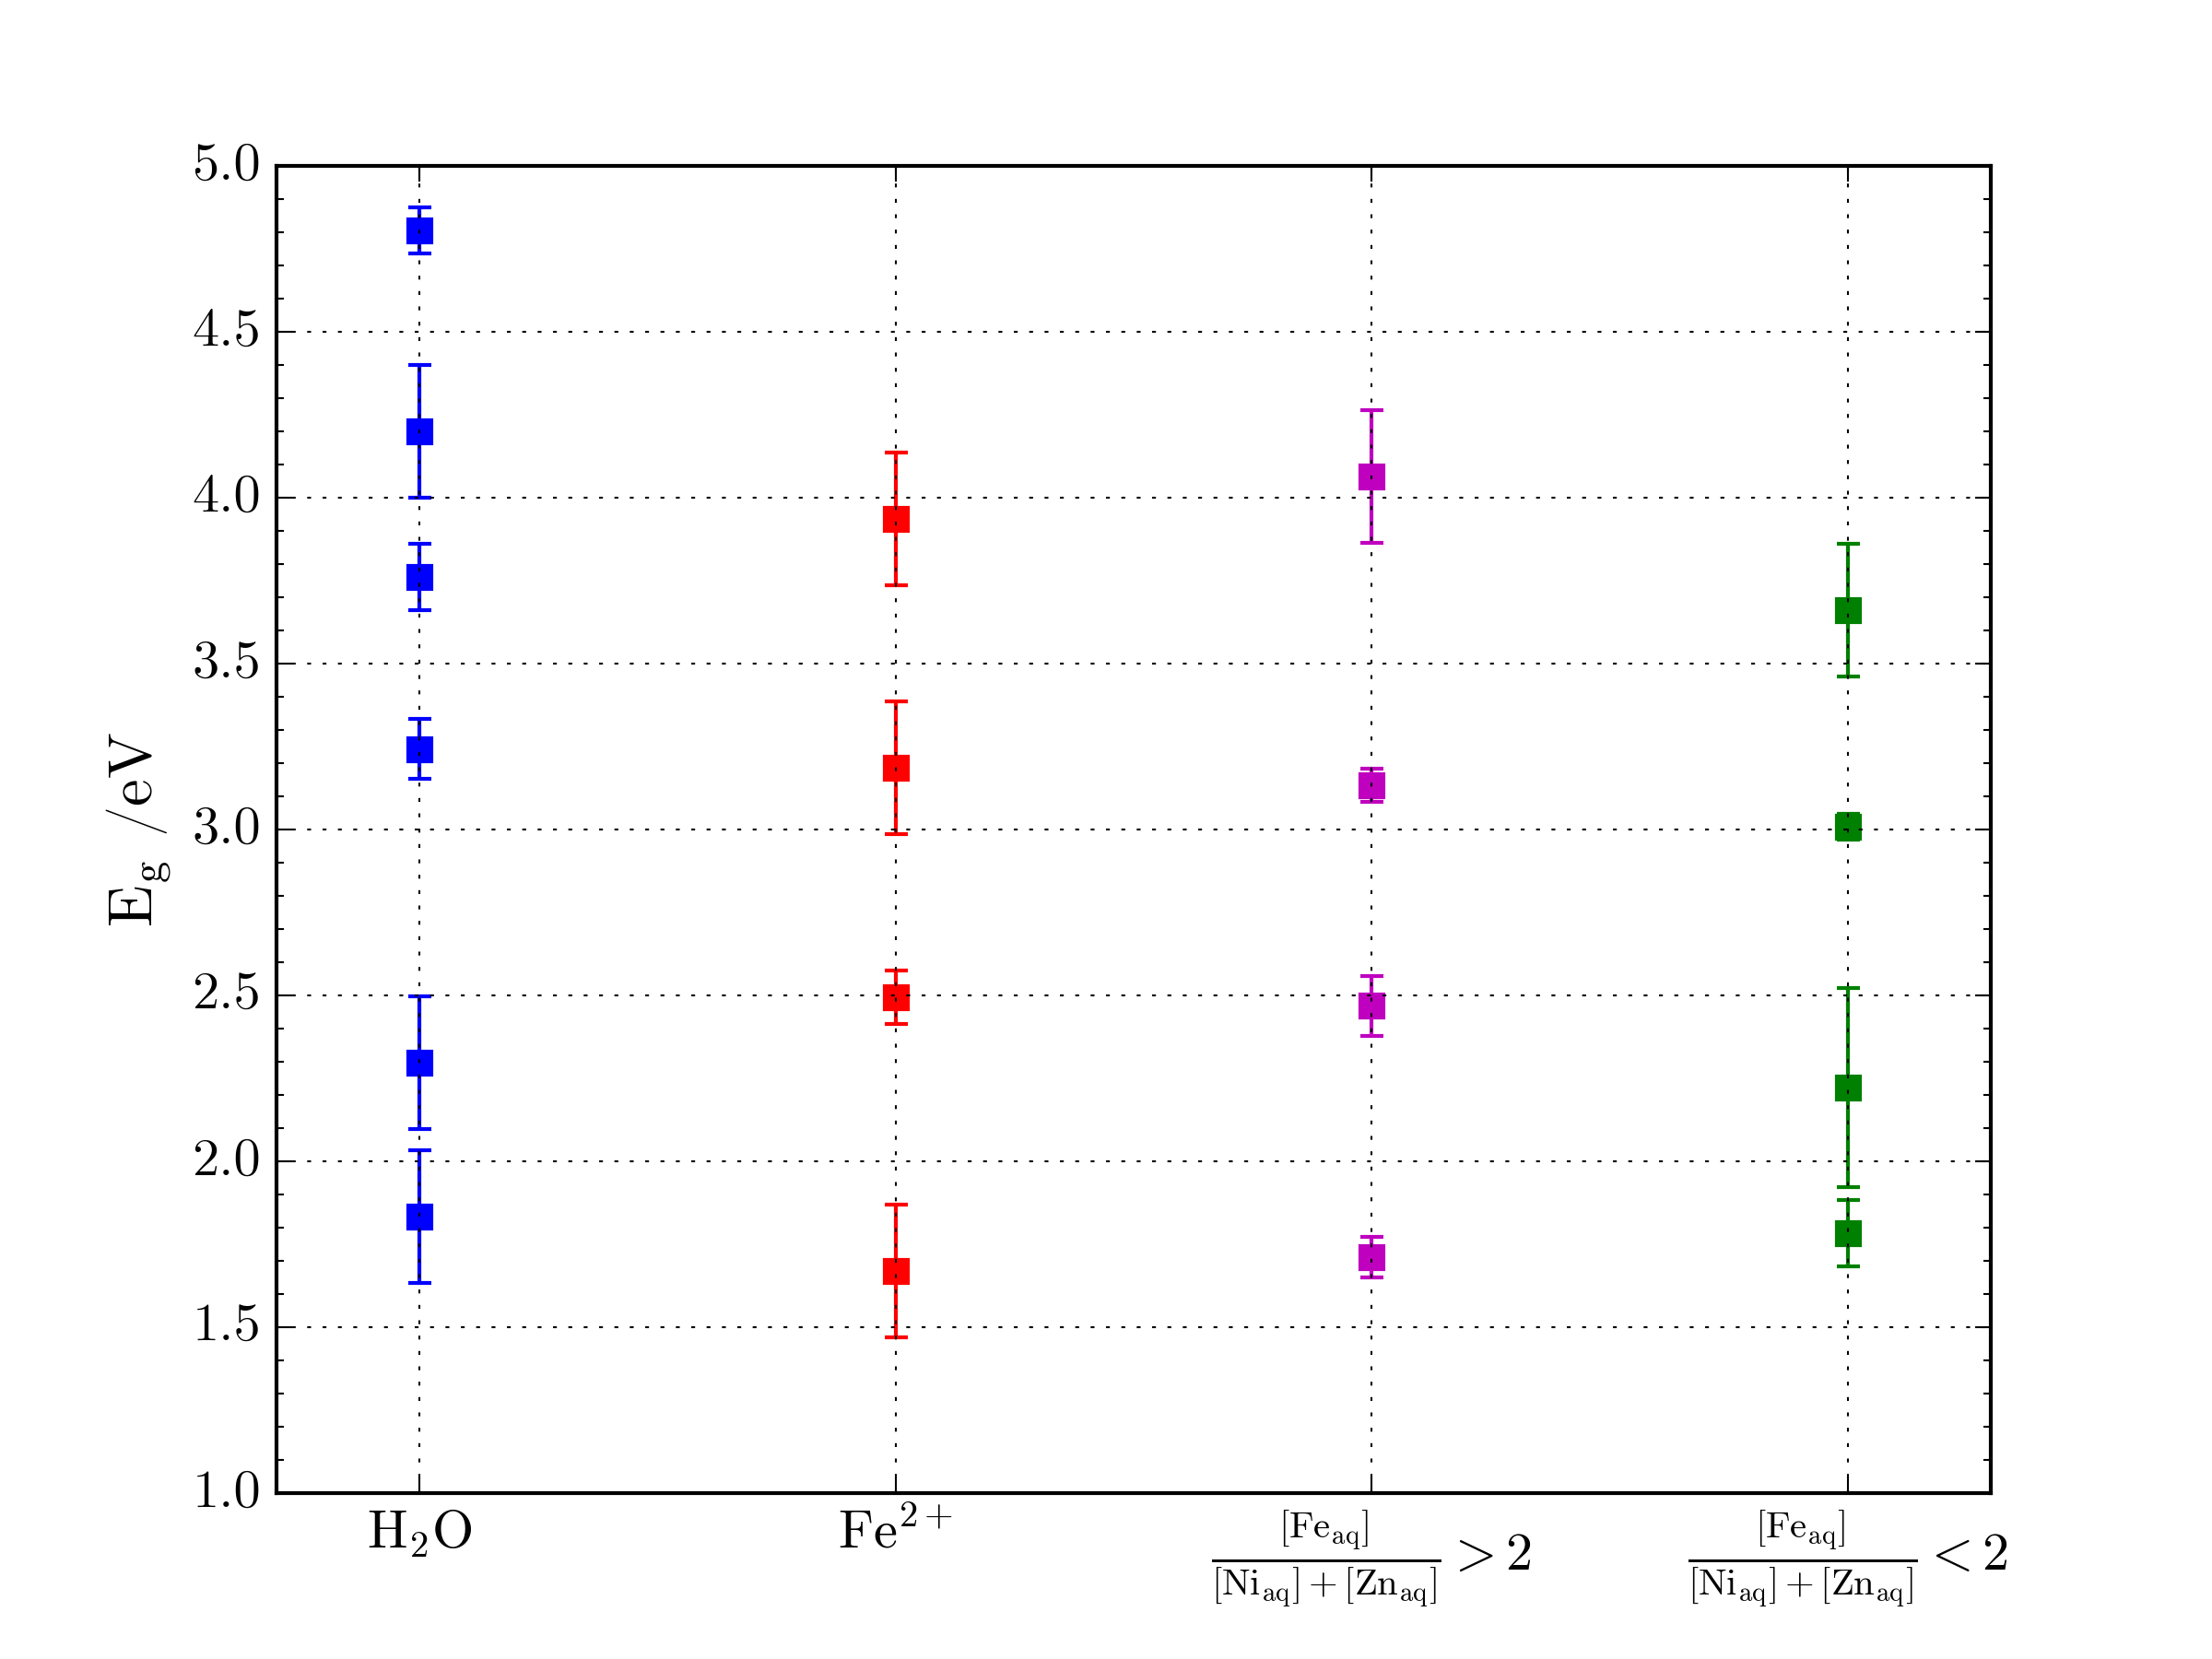
\includegraphics[width=\figwidth]{140778-PEC-Fit-Zy2-Eg_vs_chemistry.png}
        \caption{Représentation graphique des valeurs de largeur de bande interdite rassemblées au tableau
        \ref{tab:ch4_band_gaps_fit_Zy2}.}
        \label{fig:ch4_Eg_Zy2_graph}
    \end{figure}    


    \subsection{Synthèse des résultats}\label{subsec:ch4_summary_impurities}


    Les mesures de courant de couplage à 280°C ont montré que les densités de courant de couplage les plus élevées sont
    obtenues pour les électrolytes les plus chargés en cations de fer, l’effet de ces derniers semblant plus marqué
    lorsqu’ils sont associés à des cations nickel et zinc en plus faibles concentrations. Ces observations, en accord
    avec les résultats des mesures des épaisseurs de zircone atteintes en fin d’expérience, suggèrent que les impuretés
    en fer, nickel et zinc dans un rapport molaire initial de concentrations dans l’électrolyte tel que
    \ratio\ soit supérieur à 2 sont néfastes pour la résistance à la corrosion du Zy2. Ce dernier constat
    va à l’encontre des conclusions du retour d’expérience de l’incident du réacteur KKL \citep{Edsinger2004}, mais il faut rappeler que
    ce retour d’expérience concernait des oxydations en réacteur sous irradiation.

    Par ailleurs, il semble raisonnable de conclure des mesures des épaisseurs de zircone atteintes en fin d’expérience
    qu’un contact galvanique avec l’Inc718 accroît la corrosion du Zy2 dans un électrolyte chargé en cations fer. 
    
    La présence de cations fer dans l’électrolyte des micro-autoclaves a également une influence sur les propriétés des
    couches d’oxydation des échantillons déduites des caractérisations photoélectrochimiques post-mortem. Les
    photovoltammogrammes indiquent que la présence de cations de fer seuls dans l’électrolyte favorise une couche
    d’oxyde plus dopée, donc plus conductrice, sur les échantillons couplés d’Inc718. Pour ces mêmes échantillons, la
    présence de cations fer dans l’électrolyte induit également l’apparition d’une phase semiconductrice non détectée
    pour les couches d’oxydation formés en eau pure, phase dont le gap (3.05 à 3.1~eV) peut correspondre à celui d’une
    spinelle de type $AB_2O_4$ telle que $FeCr_2O_4$. Ce phénomène n’est pas observé dans le cas des échantillons couplés de
    Zy2, mais on note que la présence de nickel et/ou de zinc dans l’électrolyte favorise la formation de phases dont la
    largeur de bande interdite est inférieure à 3.5~eV telles que l’hématite et un spinelle de type $FeCr_2O_4$.
    
    Si les résultats résumés ci-dessus nous semblent très intéressants, il nous faut reconnaître à ce stade qu’ils ne
    permettent pas d’avoir une idée claire des effets individuels des cations de fer, nickel et zinc sur l’oxydation des
    alliages Zy2 et Inc718, couplés ou non, en milieu désaéré. Sur les bases de ce constat et de l’évaluation du temps
    dont nous disposions, il nous a semblé plus raisonnable de limiter le nombre de paramètres d’influence dans la suite
    de notre étude. Pour l’étude de l’effet des teneurs en oxygène et en peroxyde d’hydrogène, avec illumination
    UV--Visible ou non des échantillons, sur le comportement électrochimique des alliages Zy2 et Inc718 en cellule HTP,
    nous avons donc donné la priorité aux échantillons disques et anneaux (non couplés) de Zy2 et d’Inc718 exposés en
    micro-autoclaves dans l’électrolyte de référence c’est-à-dire l’eau (initialement) pure, des conditions
    expérimentales que nous désignerons par conditions de chimie "normales".


    \section{Effets des teneurs en $O_2$ et $H_2O_2$ de l’électrolyte: étude en cellule HTP}\label{sec:ch4_oxygen_effect}

    \subsection{Conditions expérimentales}\label{subsec:ch4_exp_cond_oxygen}
    
    Pour mémoire, les schémas de la cellule HTP et du porte-échantillon correspondant sont présentés au chapitre
    \ref{chap:design} (figure \ref{fig:Profile_HT_cell}),
    et une vue schématique des différentes géométries d’échantillon utilisées est disponible au chapitre \ref{chap:methods} (figure
    \ref{fig:ch2_samples_schemes}). Les disques et les anneaux sont positionnés face à face à une distance de 2~mm l’un de l’autre, et sont
    instrumentés de manière à ce qu’ils puissent être étudiés par des méthodes électrochimiques. 


    Les mesures électrochimiques ont été effectuées en deux campagnes sur les échantillons de Zy2 et d’Inc718 préoxydés
    en micro-autoclave dans l’électrolyte \water . Les deux campagnes d’essai ont été réalisées avec les deux configurations
    suivantes:
    \begin{itemize}
        \item première campagne d’essai : 718 (disque) / Zy2 (anneau)
        \item deuxième campagne d’essai : Zy2 (disque) / 718 (anneau)
    \end{itemize}


    Les mesures de potentiel à l’abandon des échantillons de Zy2 et Inc718, sous illumination UV--Visible continue ou
    non, présentées au paragraphe \ref{subsec:ch4_oxygen_ECP} concernent des géométries de type disque. Les courbes de polarisation présentées
    au paragraphe \ref{subsec:ch4_oxygen_Tafel} ont également été obtenues avec des géométries d’échantillon de type disque ; pour ces dernières
    mesures, la contre-électrode était le corps de la cellule HTP.
    
    Comme déjà mentionné au chapitre \ref{chap:design} (\S \ref{subsec:ch4_oxygen_ZRA}), la géométrie 
    de type disque a l’avantage de limiter les
    effets de bord dans l’évaluation de la surface exposée à l’électrolyte, et également de maximiser le flux lumineux
    arrivant sur l’échantillon à travers le hublot de saphir. Les illuminations UV--Visible intenses et continues ont été
    réalisées avec la lampe Hg dont le flux lumineux émis couvre un domaine de longueurs d’onde allant du visible aux
    UV.
    
    Pour réaliser les mesures de courant de couplage sous illumination UV--Visible, l’utilisation d’une géométrie de type
    anneau pour le second échantillon était indispensable. Mais le flux lumineux reçu par l’anneau est plus faible que
    celui reçu par le disque, et cette géométrie induit des effets de bord. Par conséquent, l’anneau n’a été utilisé que
    pour les mesures de courant de couplage lors des deux campagnes d’essai. Les résultats présentés au paragraphe
    \ref{subsec:ch4_oxygen_ZRA}
    ont été obtenus lors de la deuxième campagne d’essais.
    
    L’ensemble des mesures électrochimiques mentionnées ci-dessus a été réalisé en suivant les protocoles expérimentaux
    décrits au chapitre \ref{chap:methods} (\S \ref{sec:ch2_electrochemistry}). L’électrolyte était constitué d’eau ultra-pure désaérée à l’argon, ou d’eau
    ultra-pure contenant soit 200~ppb d’oxygène dissous, soit 200~ppb d’oxygène et 400~ppb de peroxyde d’hydrogène
    dissous. Ce dernier cas correspond aux conditions dites « standards » de fonctionnement d’un réacteur à eau
    bouillante (chapitre \ref{chap:ch1_bib}, tableau \ref{tab:operating_parameters_reactors} et figure \ref{fig:radiloytic_species_profil}). 

    
    
    \subsection{Potentiels électochimiques à l'abandon}\label{subsec:ch4_oxygen_ECP}

    La figure \ref{fig:ch4_ECP_Zy2_UV_ON_OFF} ainsi que la figure \ref{fig:ch4_ECP_718_UV_ON_OFF} 
    illustrent l’évolution avec le temps des potentiels électrochimiques à
    l’abandon pour les échantillons de Zy2 et Inc718, respectivement, au cours d’alternances obscurité/illumination
    UV--Visible. La figure \ref{fig:ch4_dE_UV_ON_OFF} représente l’évolution avec le temps de la différence de potentiel entre les deux
    matériaux, déterminée à partir des données expérimentales des figures \ref{fig:ch4_ECP_Zy2_UV_ON_OFF} et \ref{fig:ch4_ECP_718_UV_ON_OFF}.
    

    L’examen de ces figures montre tout d’abord que le potentiel électrochimique initial (à l’obscurité) de
    l’échantillon d’Inc718 est systématiquement supérieur à celui de l’échantillon de Zy2. Dans les conditions de
    l’expérience, l’Inc718 peut donc être qualifié de matériau plus "noble" que le Zy2. Le couplage galvanique des
    deux matériaux se traduira globalement par une réaction d’oxydation sur l’échantillon de Zy2 et une réaction de
    réduction l’échantillon d’Inc718.
    
    Par ailleurs, on note qu’en présence d’oxygène dissous, le potentiel électrochimique initial (à l’obscurité) de
    l’Inc718 prend des valeurs plus anodiques, et encore plus anodiques lorsque du peroxyde d’hydrogène est également
    dissous. Cet effet est nettement moins prononcé dans le cas de l’échantillon de Zy2. 
    
    On peut également observer que, lors des transitions obscurité/illumination UV--Visible, le potentiel électrochimique
    des deux matériaux prend des valeurs plus cathodiques, quelle que soit la composition d’électrolyte. Ces
    observations indiquent que les couches d’oxydes formées sur les deux matériaux présentent globalement une
    semiconduction de type \emph{n}, en accord avec les résultats issus des caractérisations photoélectrochimiques exposées au
    paragraphe \ref{subsec:post_mortem_PEC}.


    Même si l’évolution du potentiel avec le temps, au cours de l’alternance obscurité puis illumination UV--Visible, diffère
    selon les conditions expérimentales (échantillon, électrolyte), le photopotentiel (défini comme l’écart entre le
    potentiel sous illumination et le potentiel à l’obscurité) est en valeur absolue plus grand en présence qu’en
    absence d’oxygène dissous, et encore plus grand lorsque le peroxyde d’hydrogène est également présent dans
    l’électrolyte.
    
    Il ressort des observations précédentes que la différence de potentiel entre les deux matériaux placés dans les
    mêmes conditions d’électrolyte augmente en présence d’oxygène dissous, et ce davantage encore sous illumination
    UV--Visible. Cela suggère que le courant de couplage galvanique des échantillons augmentera en présence d’oxygène
    dissous et davantage encore sous illumination UV--Visible.

     \begin{figure}[H]
        \centering
        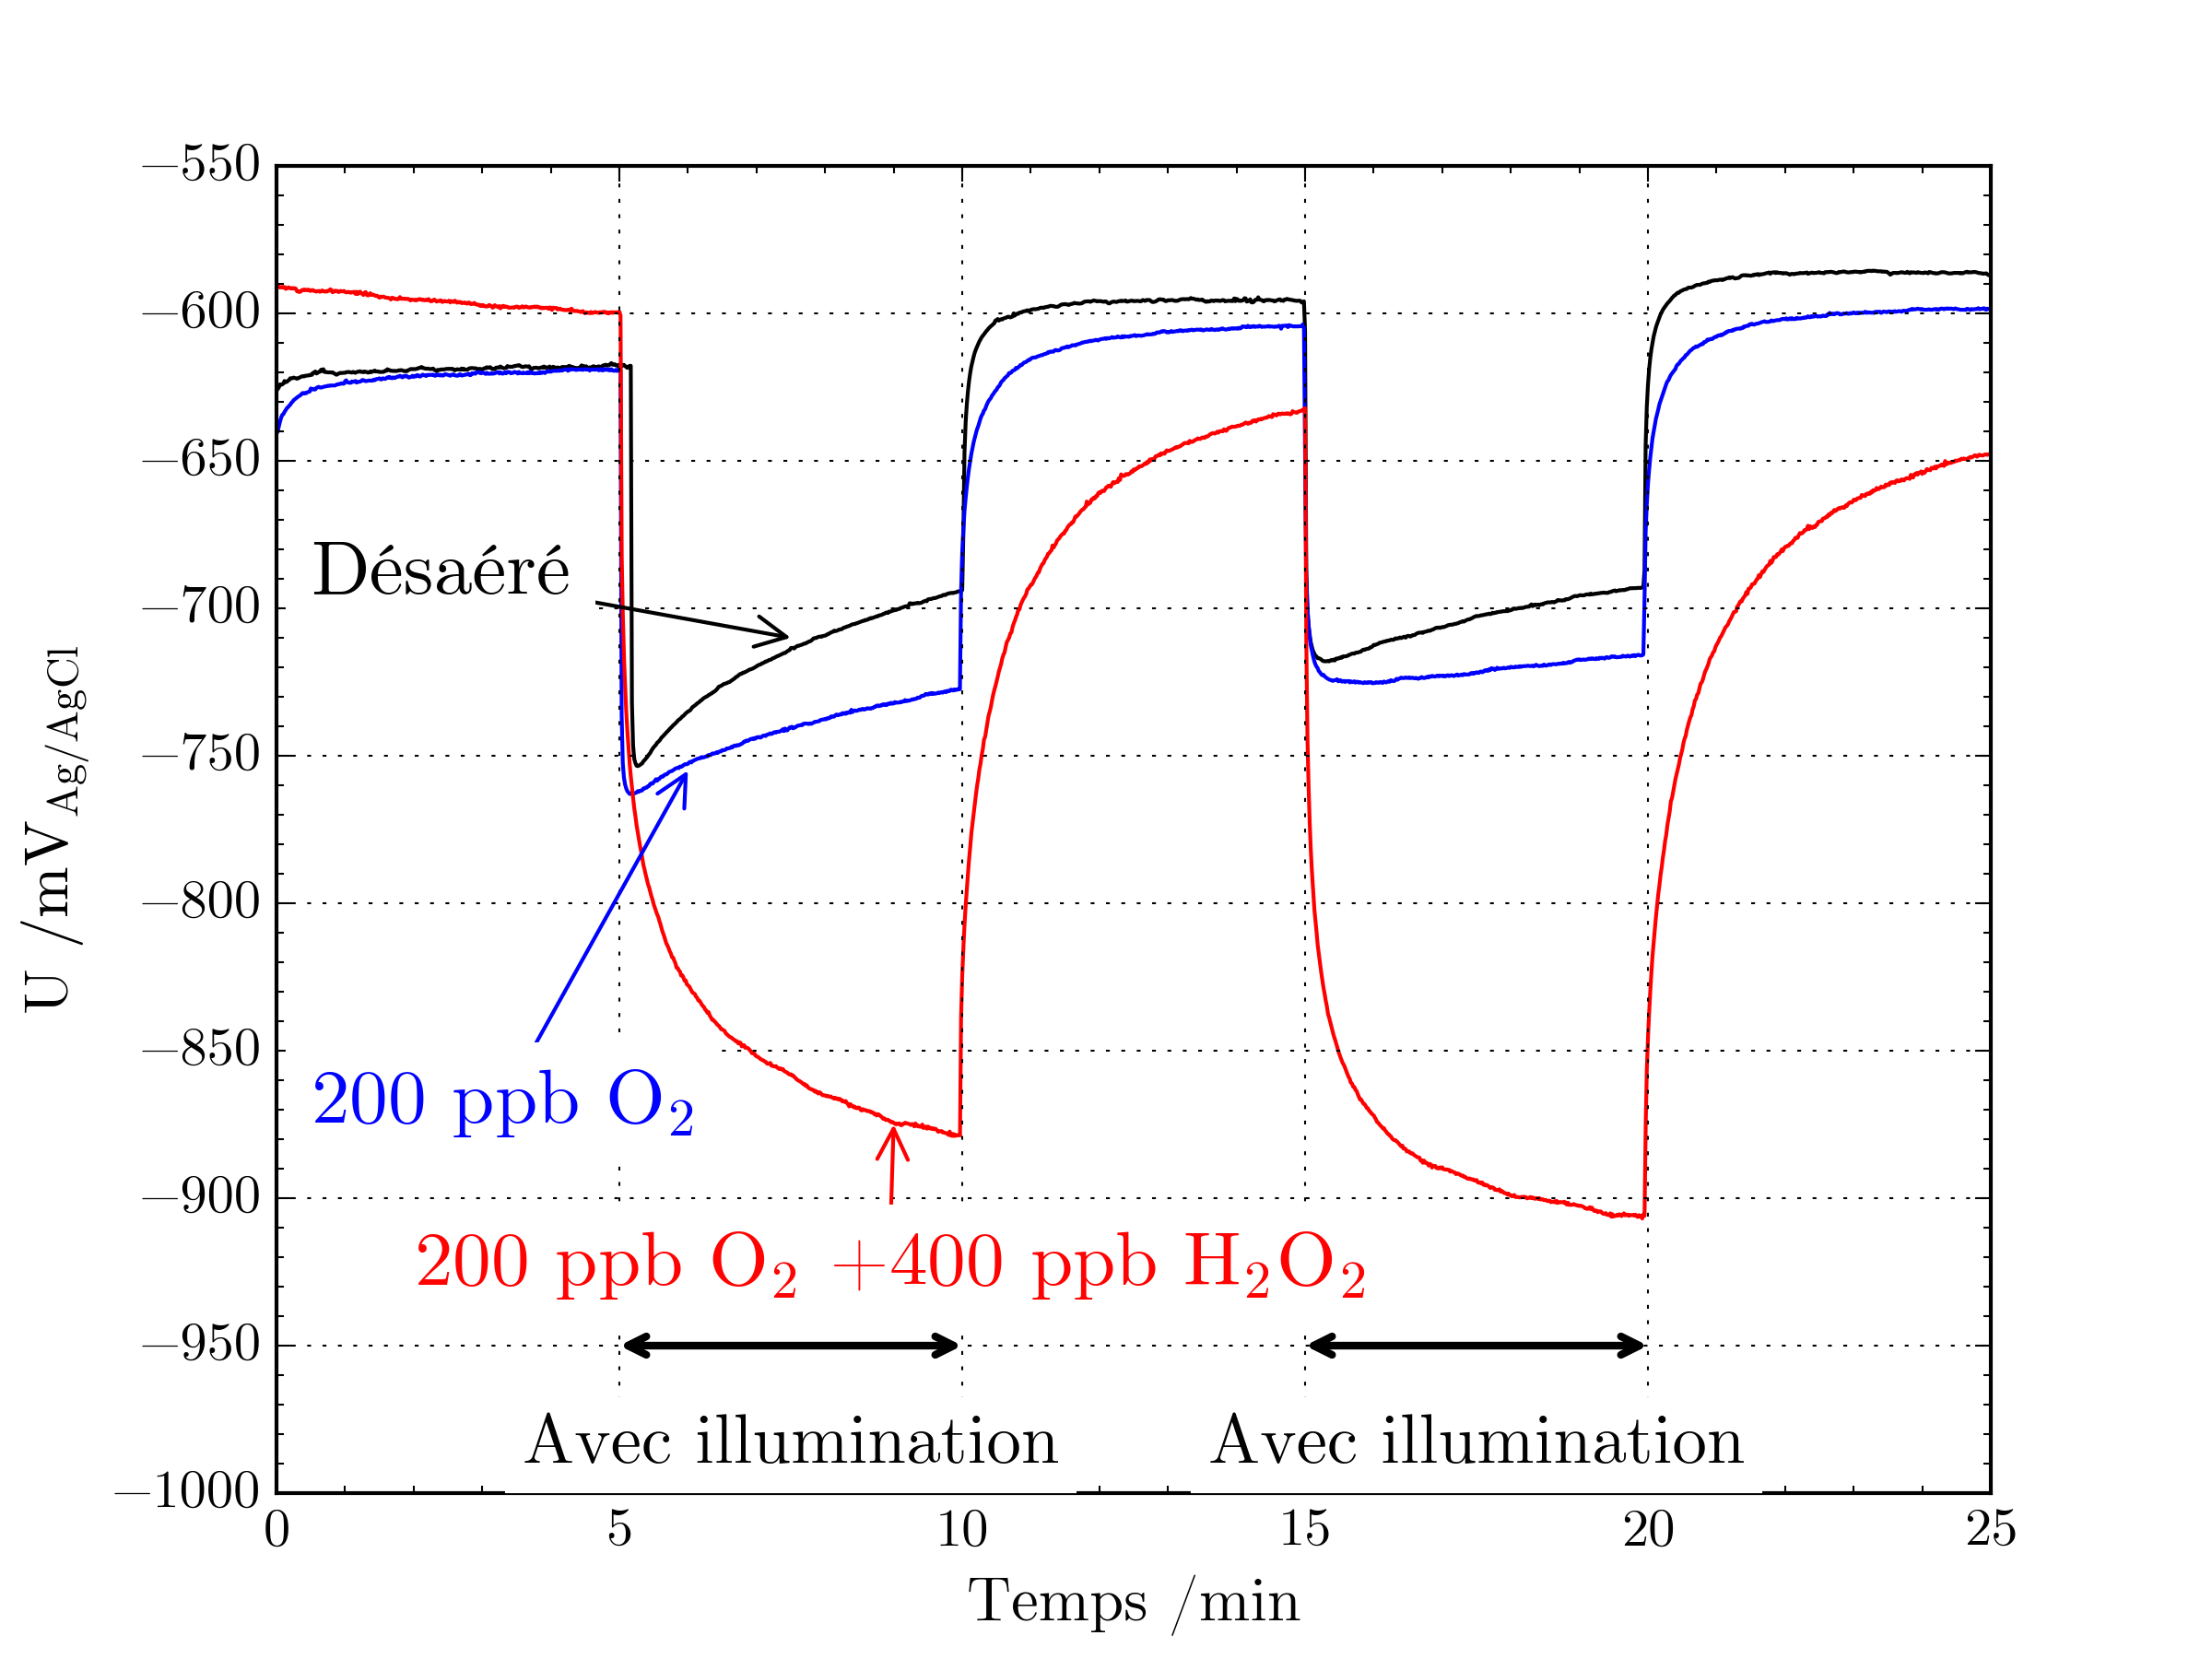
\includegraphics[width=\figwidth]{150215-chap4-ECP-Zy2-WE20-UV_ON_OFF.png}
        \caption{Evolution du potentiel électrochimique à l’abandon de l’échantillon Zy2 avec et sans illumination
        UV--Visible, pour les trois électrolytes considérés. "Avec illumination" indique les périodes où l’échantillon
    est illuminé de manière continue avec la lampe Hg.}
        \label{fig:ch4_ECP_Zy2_UV_ON_OFF}
    \end{figure}

    
     \begin{figure}[H]
        \centering
        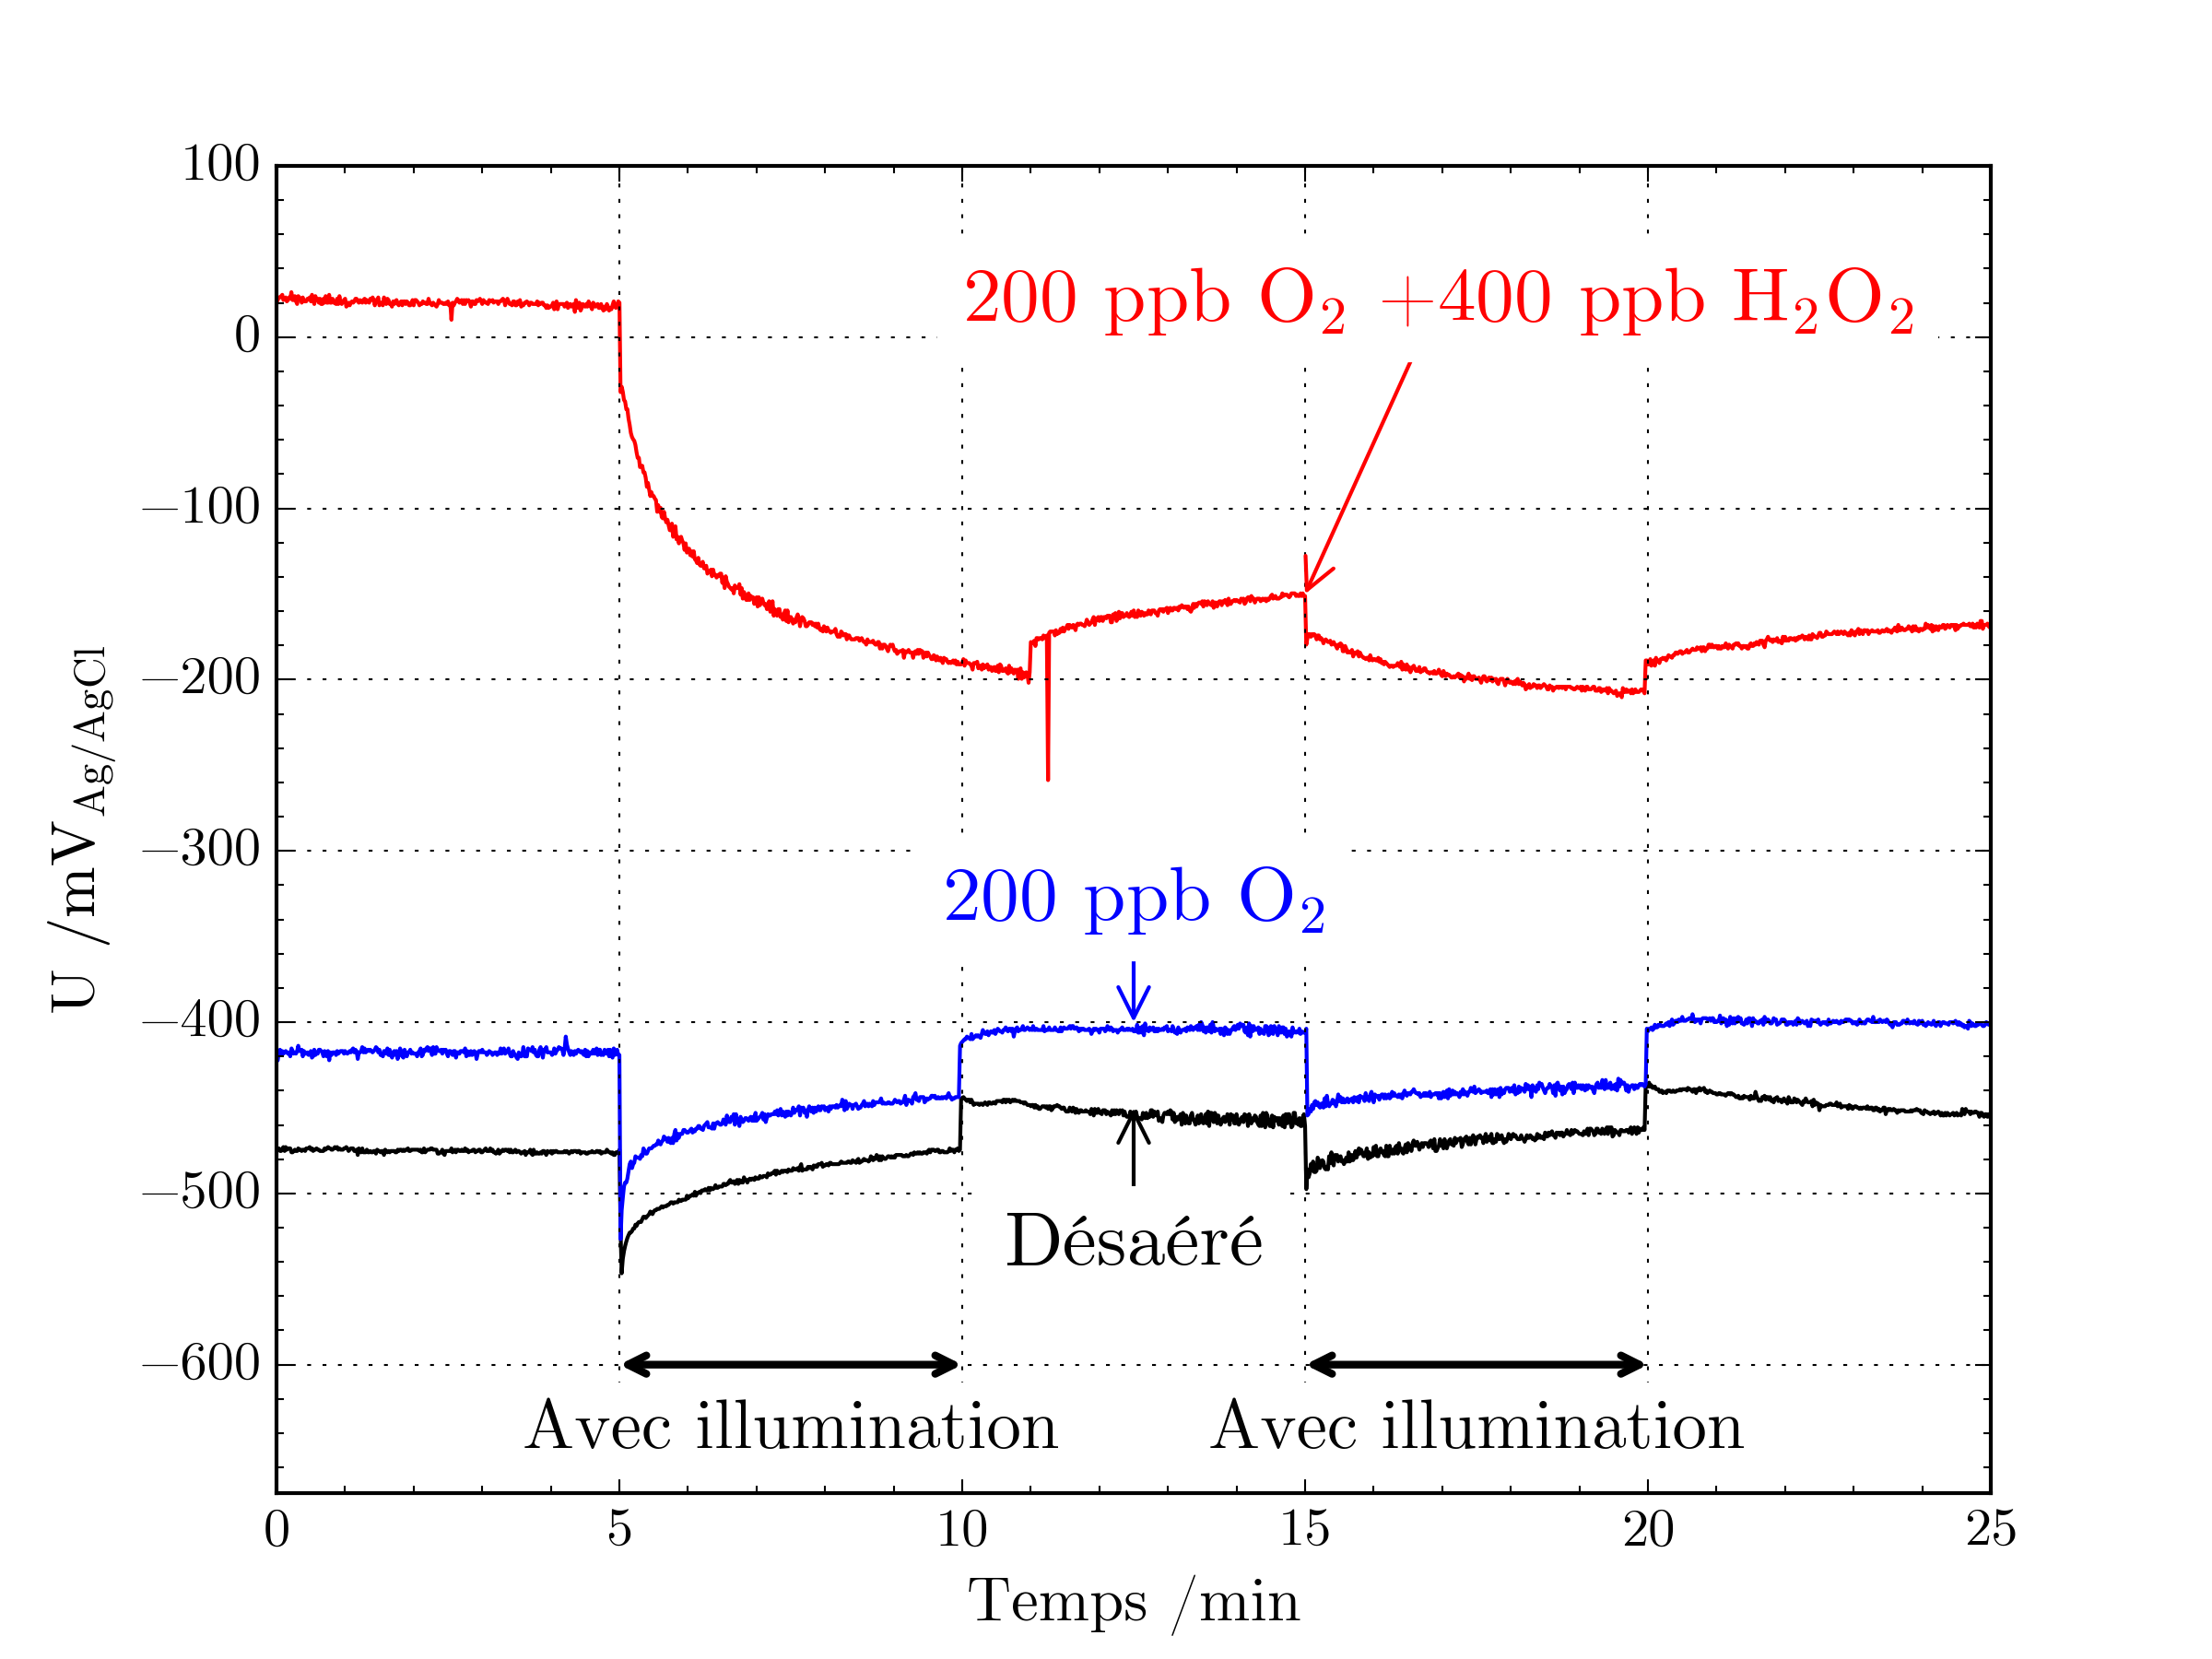
\includegraphics[width=\figwidth]{150215-chap4-ECP-Inc718-WE8-UV_ON_OFF.png}
        \caption{Evolution du potentiel électrochimique à l’abandon de l’échantillon Inc718 avec et sans illumination
        UV--Visible pour les trois électrolytes considérés. "Avec illumination" indique les périodes où l’échantillon
    est illuminé de manière continue avec la lampe Hg.}
        \label{fig:ch4_ECP_718_UV_ON_OFF}
    \end{figure}


    \begin{figure}[H]
        \centering
        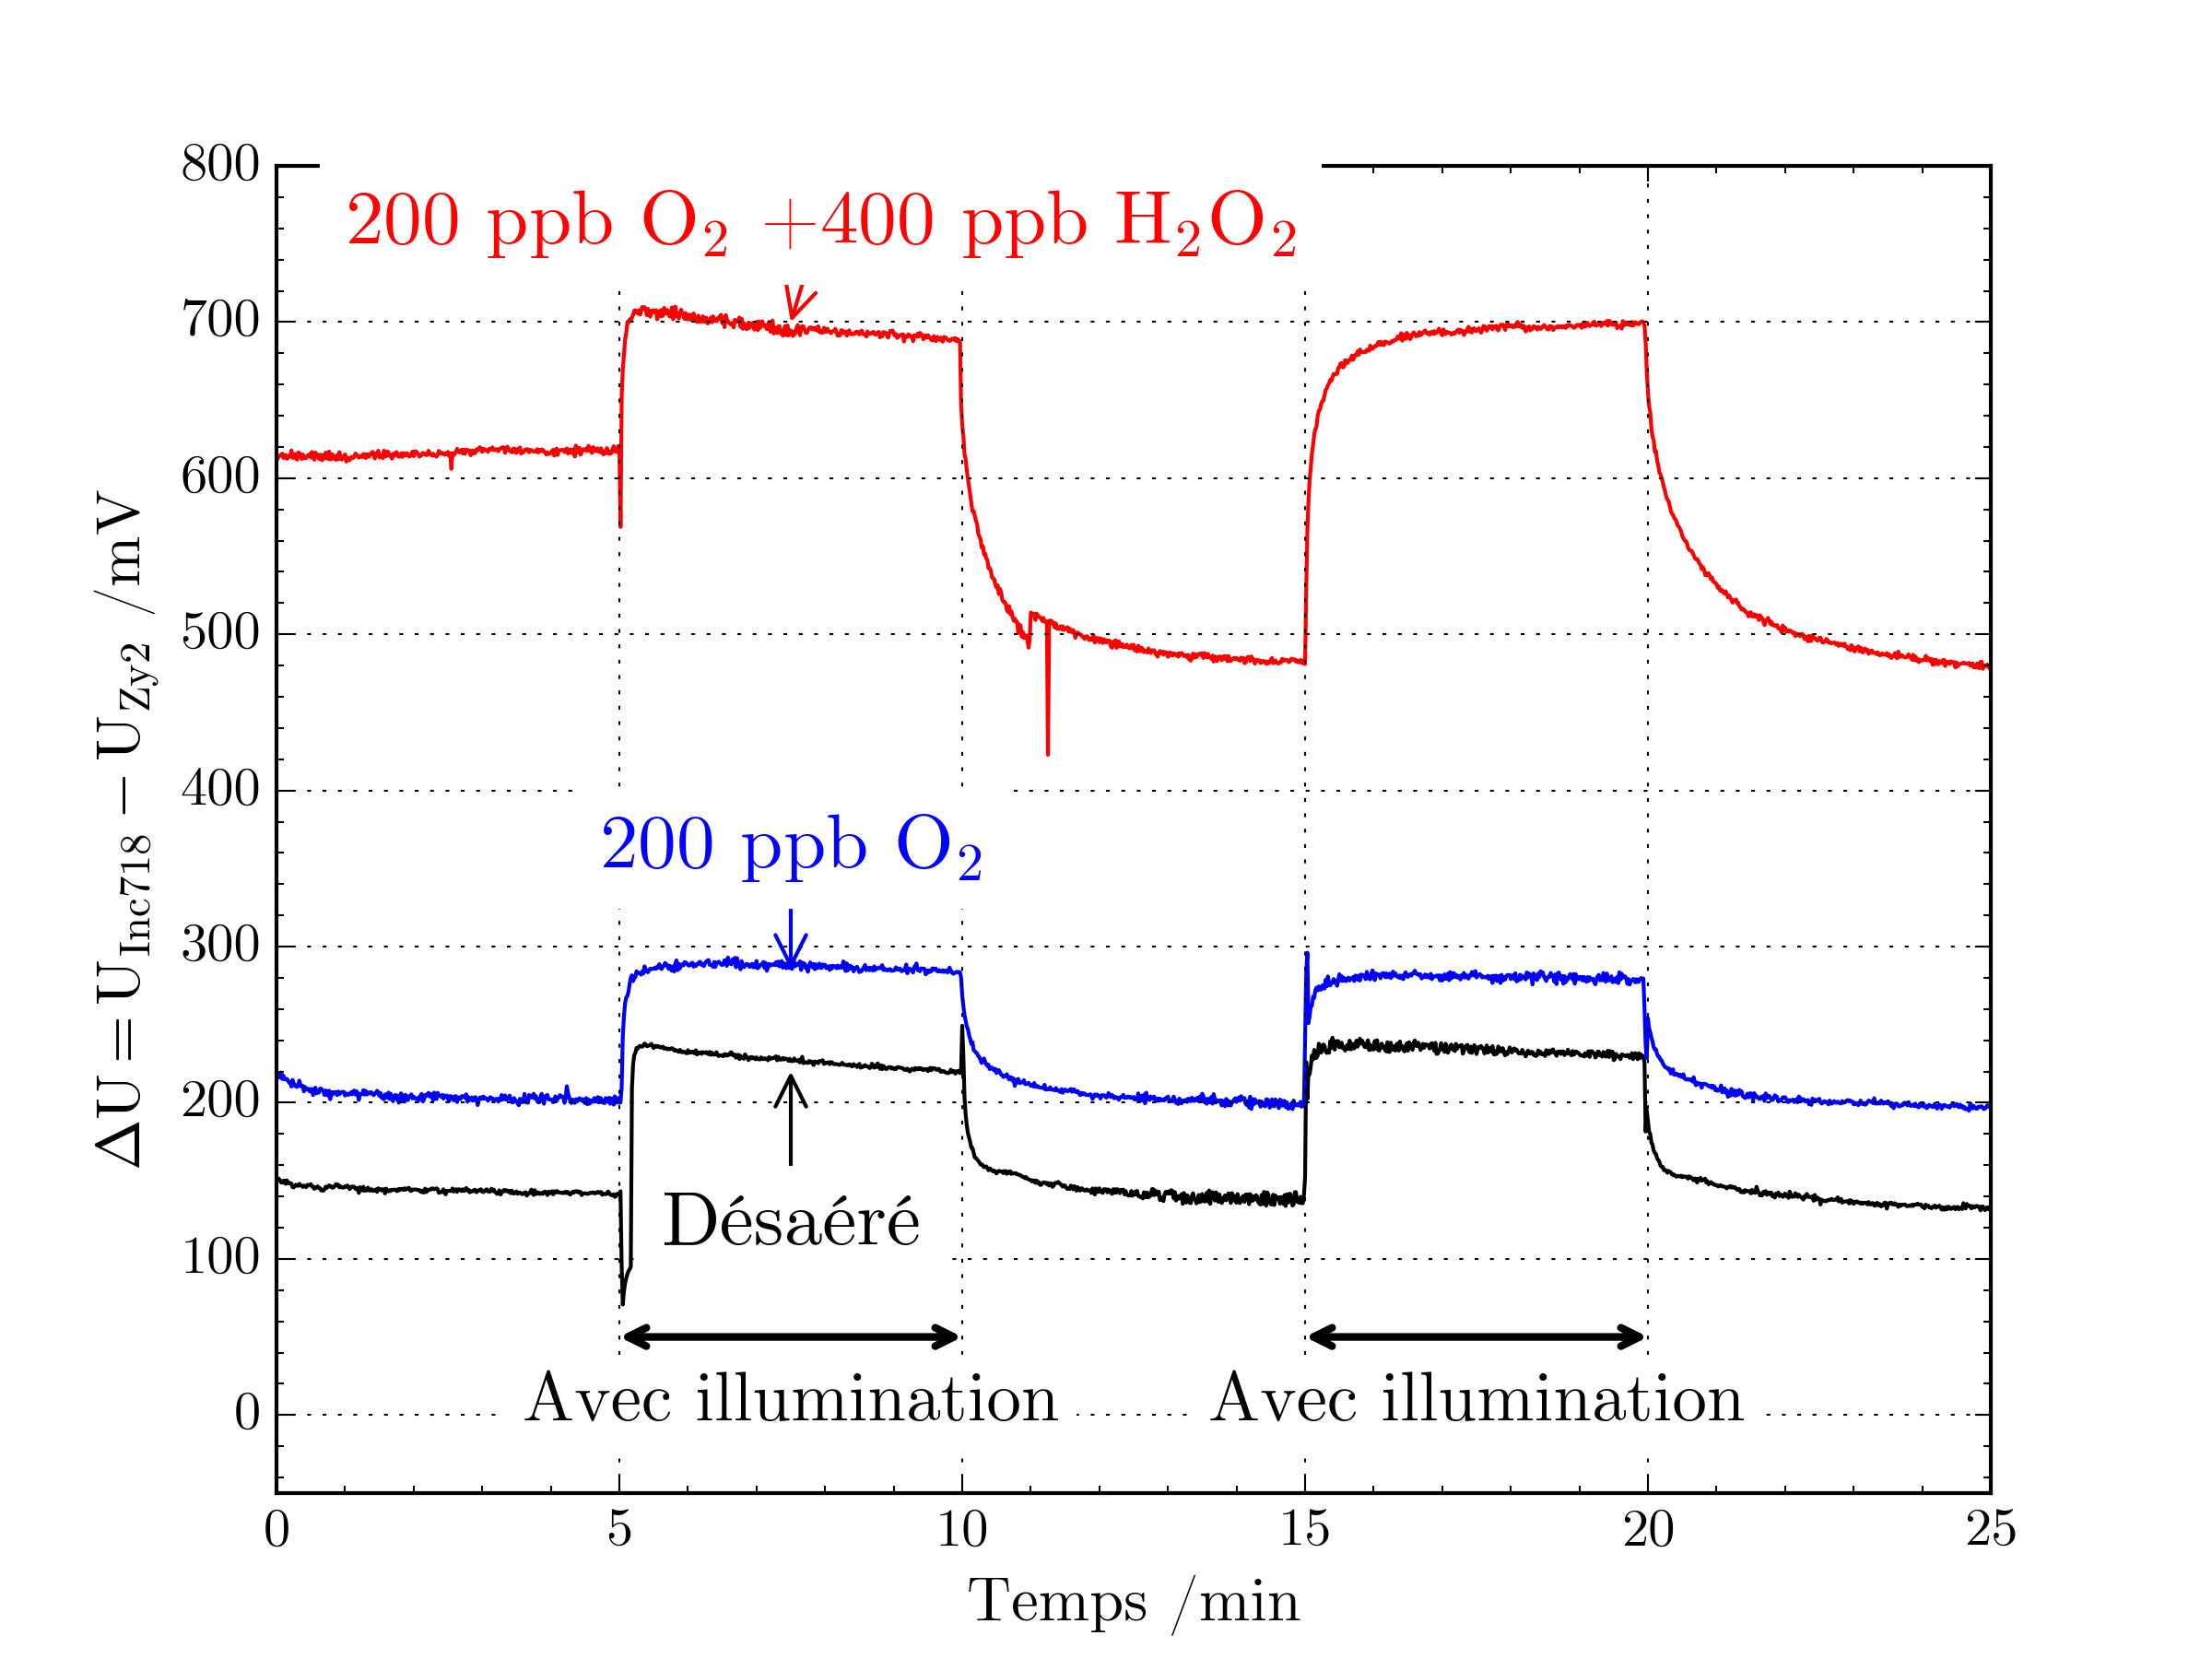
\includegraphics[width=\figwidth]{150215-chap4-dE-UV_ON_OFF.png}
        \caption{Evolution de la différence de potentiel entre les échantillons Inc718 et Zy2, déterminée à partir des
            données expérimentales de la figure \ref{fig:ch4_ECP_Zy2_UV_ON_OFF} et de la figure \ref{fig:ch4_ECP_718_UV_ON_OFF}.
            "Avec illumination" indique les périodes où l’échantillon est illuminé de manière continue avec la lampe Hg.}
        \label{fig:ch4_dE_UV_ON_OFF}
    \end{figure}

    Comme indiqué plus haut, la différence de potentiel à l’abandon avec et sans illumination UV--Visible est appelée
    photopotentiel, $U_{ph}$. En valeur absolue, ce dernier peut être au relié à la densité de photocourant, $j_{ph}$, et à la densité
    de courant d’échange à l’obscurité, $j_0$, selon l’Équation \ref{eq:ch4_Uph_Iph} \citep{Memming2008}:

    \begin{equation}
        \vert U_{ph} \vert = \frac{kT}{e} \ln \left( \frac{\vert j_{ph}\vert}{j_0} + 1 \right)
        \label{eq:ch4_Uph_Iph}
    \end{equation}

    Cette relation suggère que plus le photopotentiel est élevé, plus le photocourant sera élevé. Il convient cependant de
    souligner que l’établissement de cette relation fait appel à un certain nombre d’hypothèses simplificatrices, par
    exemple illumination monochromatique, pas de limitation au transfert et pas de recombinaisons des paires électron--trou
    photogénérées, hypothèses peu plausibles ici, ne serait-ce que parce que l’illumination mise en oeuvre est
    polychromatique. Néanmoins, avec toutes les précautions d’usage, la relation \ref{eq:ch4_Uph_Iph} pourrait nous être utile dans l’analyse
    des photocourants au paragraphe \ref{subsec:ch4_oxygen_ZRA}, qui exposent les résultats des mesures de courant de couplage à l’obscurité ou
    sous illumination UV--Visible.

    Avant de passer à l’analyse des courants de couplage, il nous parait intéressant de mentionner les mesures de
    potentiel électrochimique avec et sans illuminations UV--Visible réalisées par \citet{Kim2010} sur un alliage de
    nickel X750 qui ont été présentées dans le chapitre \ref{chap:ch1_bib} et dont les résultats sont rappelés en figure
    \ref{fig:ch4_Kim_results}. Les
    auteurs avaient observé une augmentation du potentiel électrochimique de l’alliage X750 vers des valeurs plus
    anodiques sous illumination UV--Visible traduisant une semiconduction de type \emph{p} alors que nos mesures de potentiel
    électrochimique sous illumination UV--Visible sur l’échantillon en alliage 718 (préoxydé à \SI{280}{\degreeCelsius} en eau ultra-pure
    désaéré à l’argon) ont révélé une semiconduction de type \emph{n}.

    \begin{figure}[H]
        \centering
        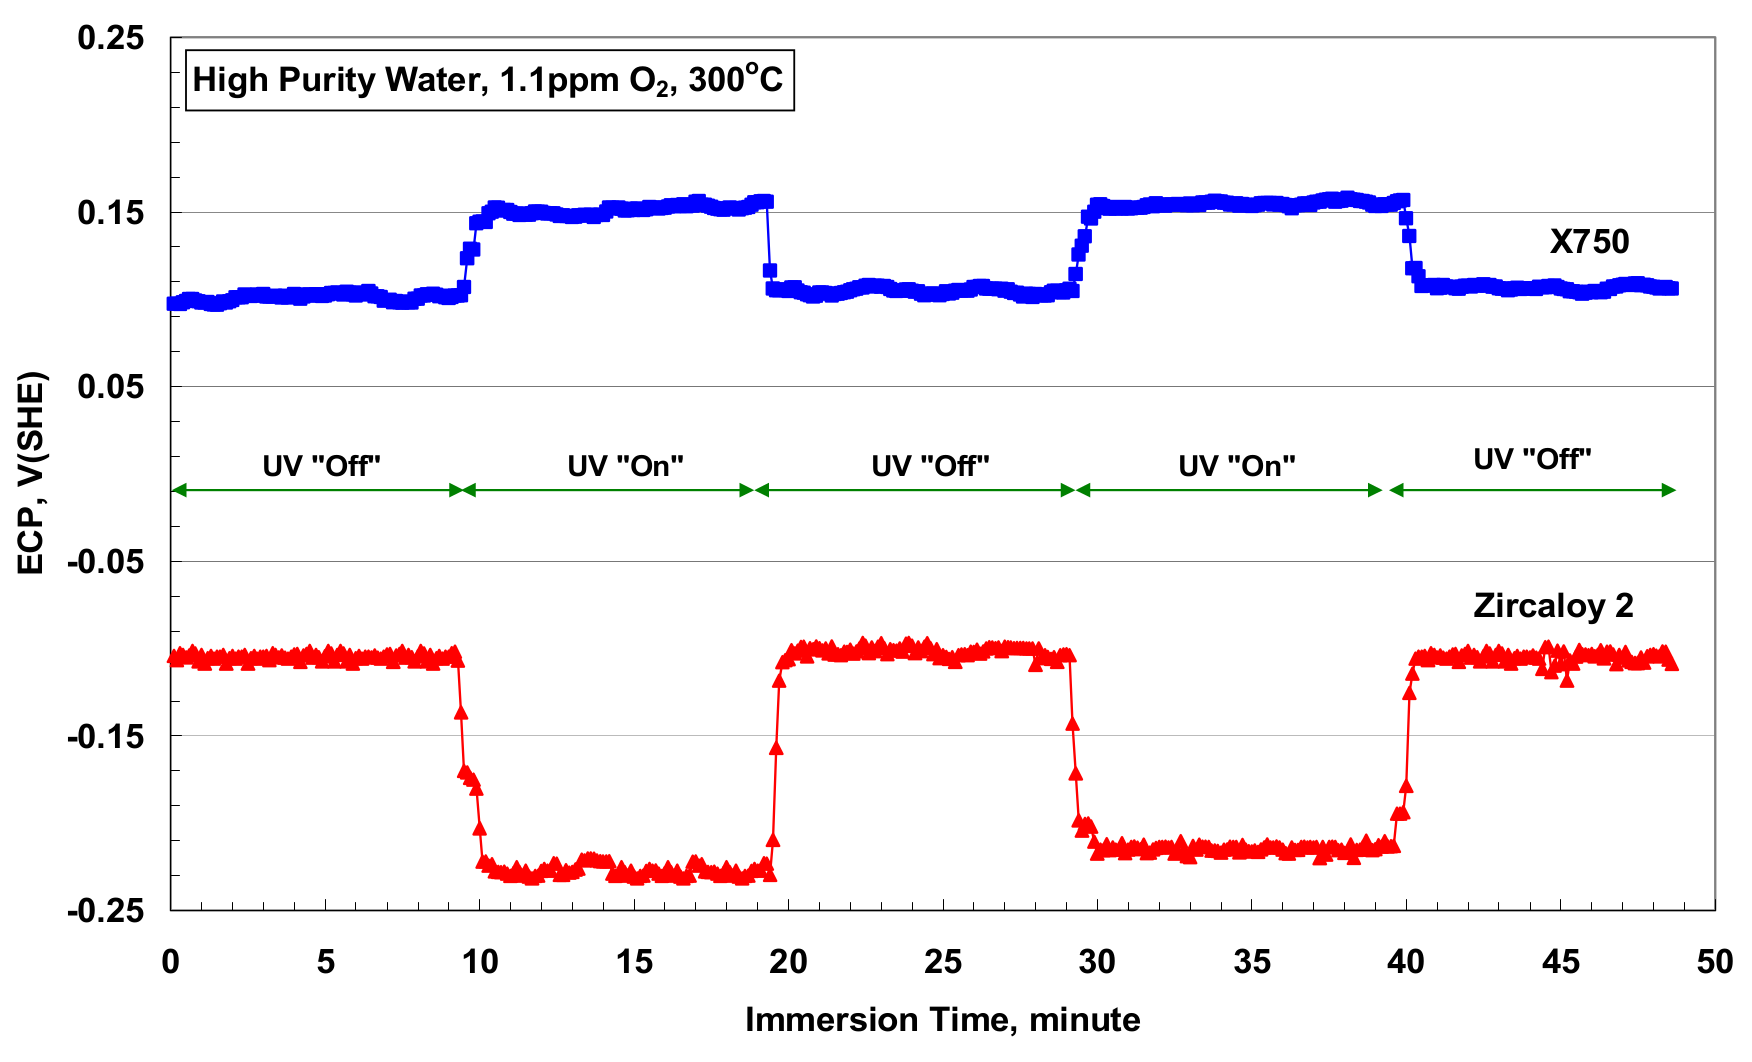
\includegraphics[width=\figwidth]{Kim_2010_Fig6.png}
        \caption[Potentiels électrochimiques mesurés sur les alliages Zircaloys-2 et X750 dans l’eau à \SI{300}{\degreeCelsius} contenant
        1~ppm d’oxygène dissous avec ou sans illumination UV--Visible.]
        {Potentiels électrochimiques mesurés sur les alliages Zircaloys-2 et X750 dans l’eau à \SI{300}{\degreeCelsius} contenant
        1~ppm d’oxygène dissous avec ou sans illumination UV--Visible \citep{Kim2010}.}
        \label{fig:ch4_Kim_results}
    \end{figure}


    Nous avons donc voulu vérifier l’évolution de potentiel électrochimique d’un échantillon en alliage de nickel X750
    avec et sans illumination UV--Visible préoxydé dans les mêmes conditions que notre échantillon en alliage de nickel
    718. La comparaison des mesures de potentiel électrochimique obtenues dans la cellule HTP à \SI{280}{\degreeCelsius} en eau ultra-pure
    contenant 200~ppb d’oxygène dissous est présentée en figure \ref{fig:ch4_comp_ECP_718_750}.
    
    On observe que l’alliage X750 présente un potentiel électrochimique plus anodique d’environ \SI{150}{\milli\volt} par rapport à
    l’alliage 718. Les deux alliages, préoxydés dans les mêmes conditions, présentent une diminution des potentiels
    électrochimiques vers des valeurs plus cathodiques lors des transitions obscurité/illumination UV--Visible traduisant
    une semiconduction de type \emph{n}. Il faut cependant noter que les transitoires obscurité/illumination UV--Visible
    semblent être plus lents dans le cas de l’alliage de nickel X750.
    
    Malgré une teneur en nickel plus importante impliquant des couches d’oxyde de nature légèrement différente,
    l’alliage X750 semble présenter un comportement très similaire à celui de l’alliage 718 sous illumination UV--Visible
    c’est-à-dire une semiconduction de type \emph{n}. A ce stade, le manque d’information sur le traitement de préoxydation
    utilisé par \citet{Kim2010} ne permet pas d’expliquer cette différence de comportement sous illumination UV--Visible.

    \begin{figure}[H]
        \centering
        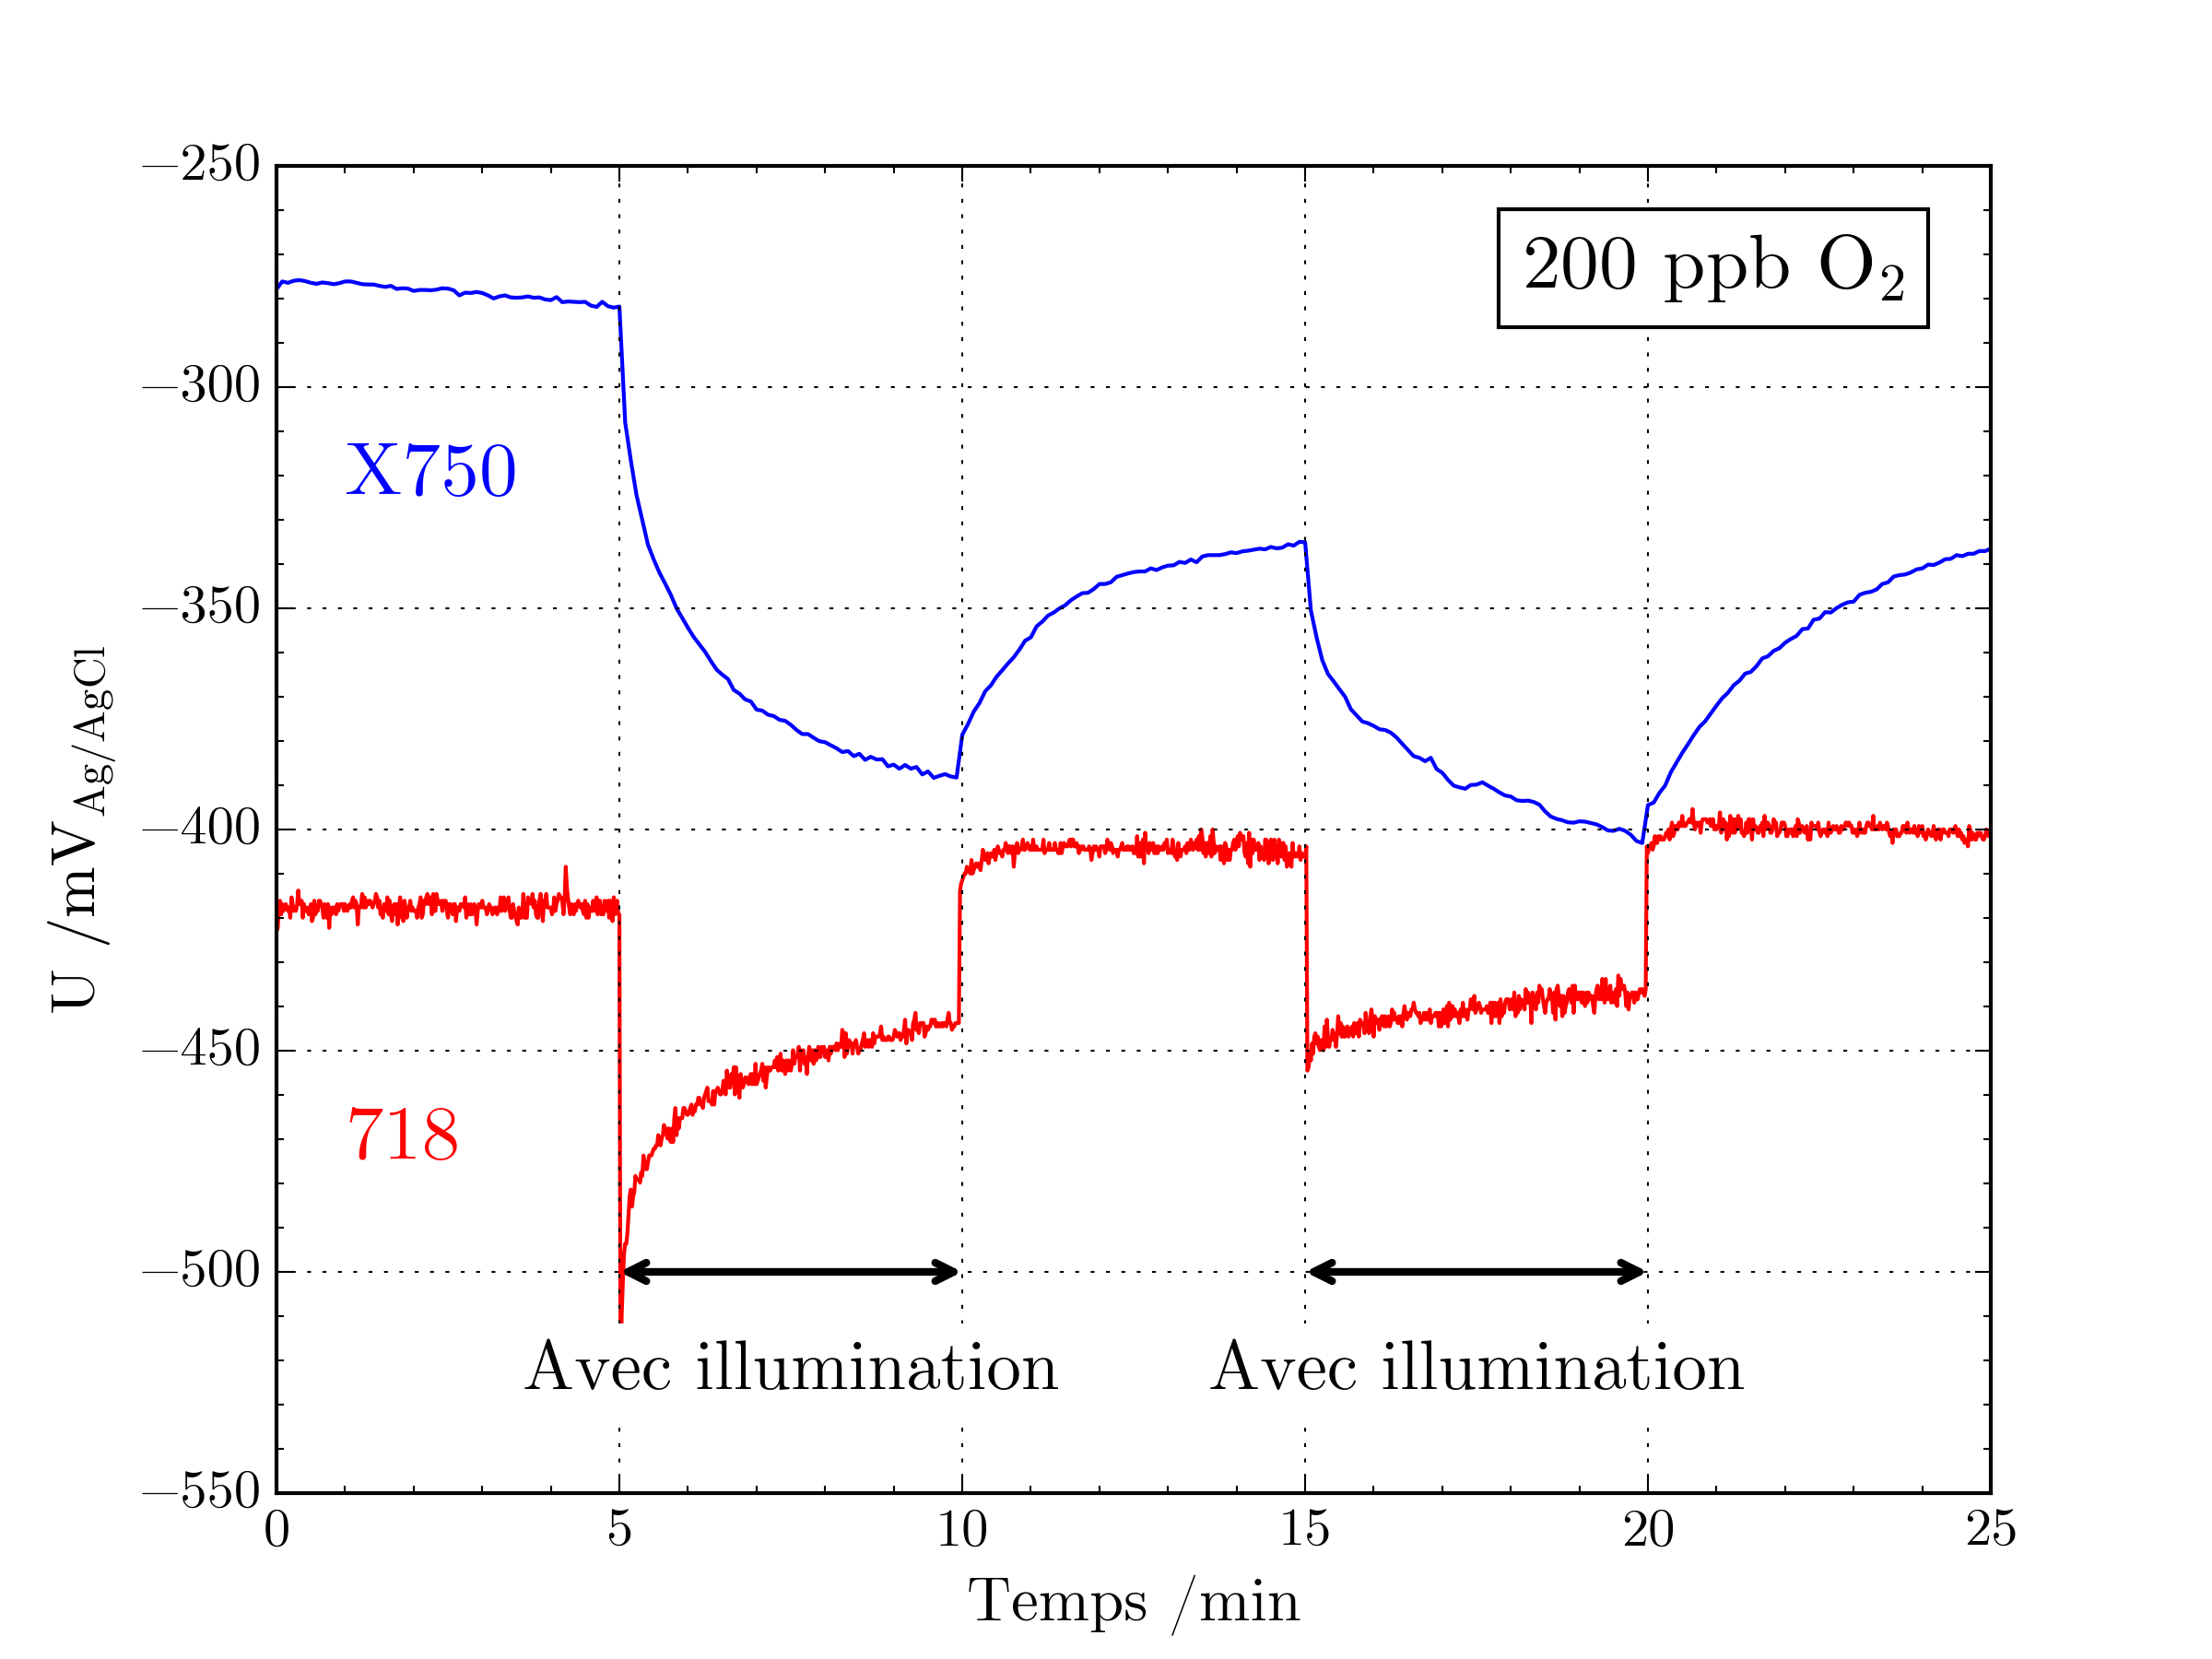
\includegraphics[width=\figwidth]{150215-chap4-ECP-Compare_X750-UV_ON_OFF.png}
        \caption{Evolution du potentiel électrochimique à l’abandon des échantillons en alliage de nickel 718 et X750
        avec et sans illumination UV--Visible à \SI{280}{\degreeCelsius} en eau ultra-pure contenant 200~ppb d’oxygène
        dissous. "Avec
    illumination" indique les périodes où l’échantillon est illuminé de manière continue avec la lampe Hg.}
        \label{fig:ch4_comp_ECP_718_750}
    \end{figure}



    \subsection{Courants de couplage}\label{subsec:ch4_oxygen_ZRA}

    La figure \ref{fig:ch4_ZRA_UV_ON_OFF} illustre l’évolution avec le temps, au cours d’alternances
    obscurité puis illumination UV--Visible, des
    densités de courant de couplage, lorsque les deux échantillons Zy2 et Inc718 sont mis en contact via un ZRA.

    \begin{figure}[H]
        \centering
        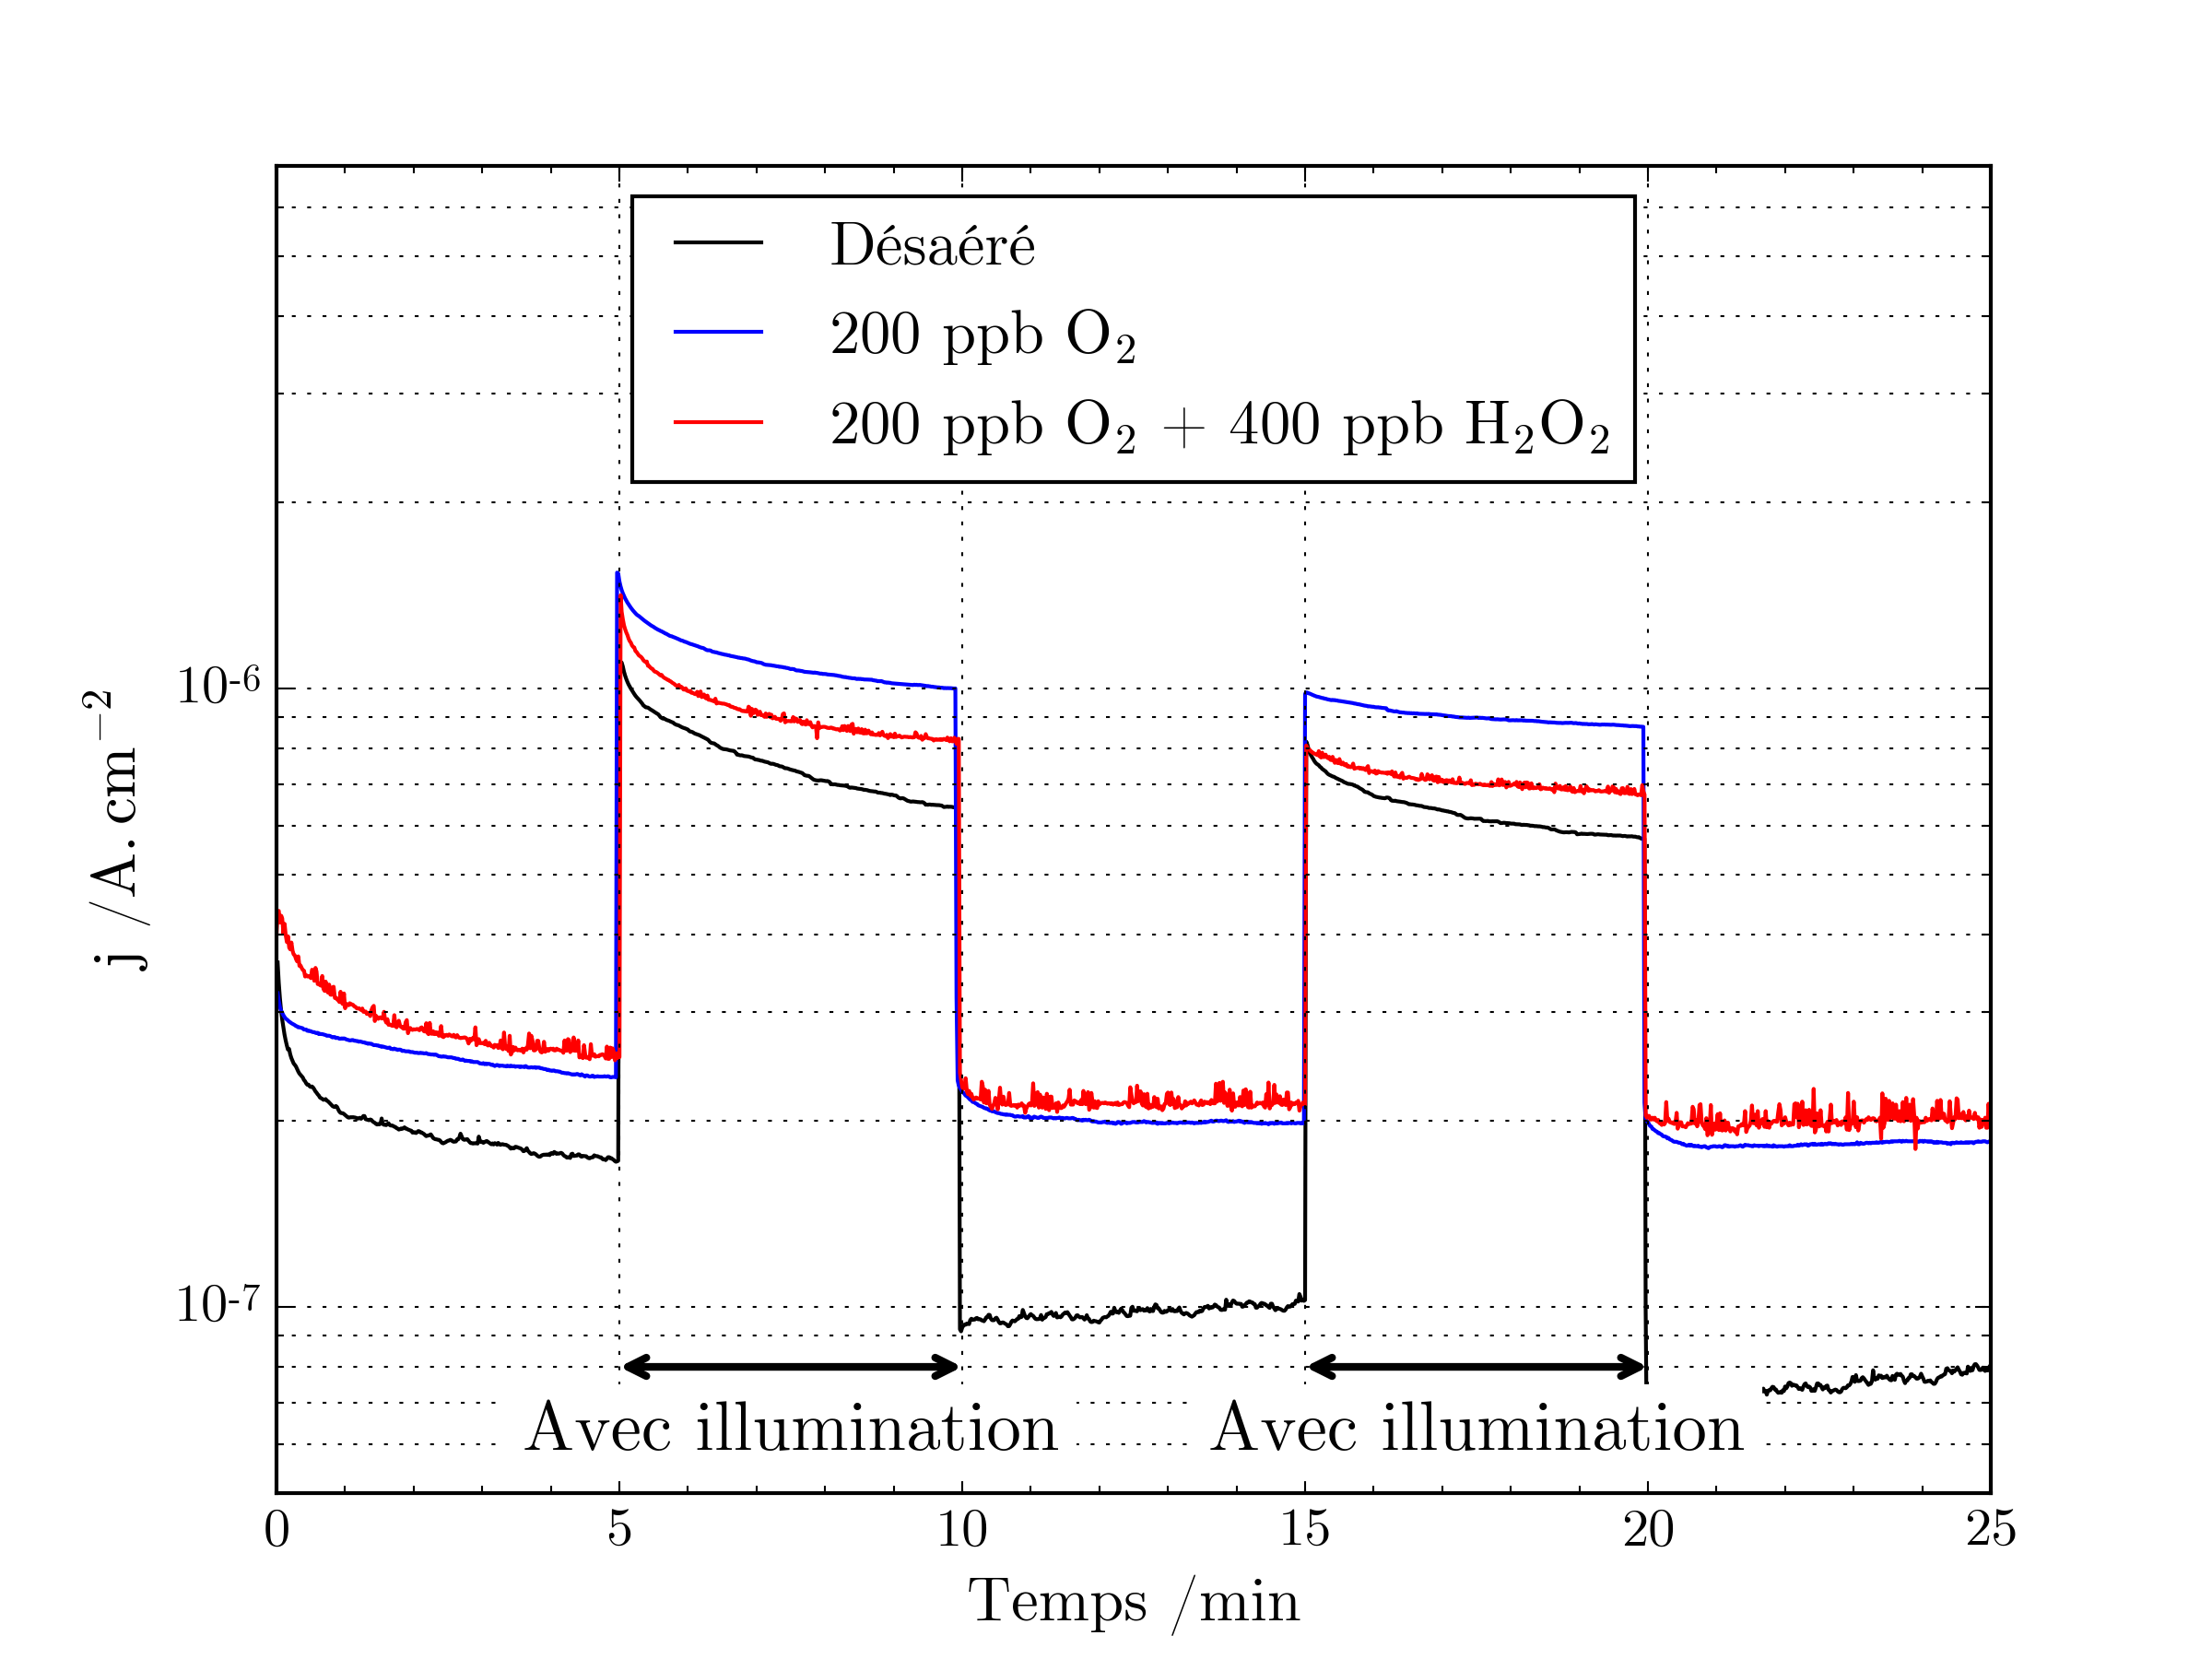
\includegraphics[width=\figwidth]{150215-chap4-ZRA-Zy2-WE20-UV_ON_OFF.png}
        \caption{Evolution de la densité de courant de couplage avec et sans illumination UV--Visible pour les trois
        électrolytes considérés. "Avec illumination" indique les périodes où l’échantillon est illuminé de manière
    continue avec la lampe Hg.}
        \label{fig:ch4_ZRA_UV_ON_OFF}
    \end{figure}

    Notons tout d’abord que le courant de couplage est positif, ce qui, compte tenu de l’arrangement des connections
    électriques des échantillons au ZRA, signifie que l’échantillon de Zy2 (resp. Inc718) est globalement le siège d’une
    oxydation (resp. réduction), comme prévu au paragraphe \ref{subsec:ch4_oxygen_ECP}.

    Par contre, contrairement à ce qui a été observé au paragraphe \ref{subsec:ch4_oxygen_ECP} pour les potentiels d’abandon, la nature de
    l’électrolyte ne semble pas avoir un impact majeur sur les courants de couplage sous illumination. Quel que soit
    l’électrolyte considéré, une augmentation d’environ un facteur 5 de la densité de courant de couplage est observée
    lors de la première illumination. En cours d’illumination, le courant de couplage diminue plus ou moins rapidement
    avec le temps. Les conditions de temps utilisées pour l’alternance obscurité/illuminations UV--Visible ne permettent
    pas de dire si le courant de couplage sous illumination finit ou non par se stabiliser, comme cela est généralement
    observé pour le photocourant généré à une interface semiconducteur/électrolyte. En effet, le photocourant à une
    interface semiconducteur/électrolyte se stabilise après une phase transitoire de réorganisation des équilibres entre
    génération de paires électron--trou, recombinaisons diverses de ces paires et transfert de charge aux espèces redox
    de l’électrolyte.

    Nous avons voulu vérifier si l’évolution du potentiel mixte en fonction de la densité de courant sous illumination
    UV--Visible présenterait une évolution logarithmique comme ce qui a été proposé au paragraphe \ref{subsec:ch4_oxygen_ECP}
    par l’équation \ref{eq:ch4_Uph_Iph}.
    Nous constatons sur la figure \ref{fig:ch4_Umix_vs_jgal} que ce n’est pas le cas mais que l’évolution est plutôt linéaire. Cet écart de
    comportement par rapport à celui prédit par l’équation \ref{eq:ch4_Uph_Iph} est très certainement lié, au moins
    partiellement, à l’utilisation d’une illumination
    polychromatique qui ne permet plus d’appliquer l’équation \ref{eq:ch4_Uph_Iph} définie pour une illumination monochromatique.

    \begin{figure}[H]
        \centering
        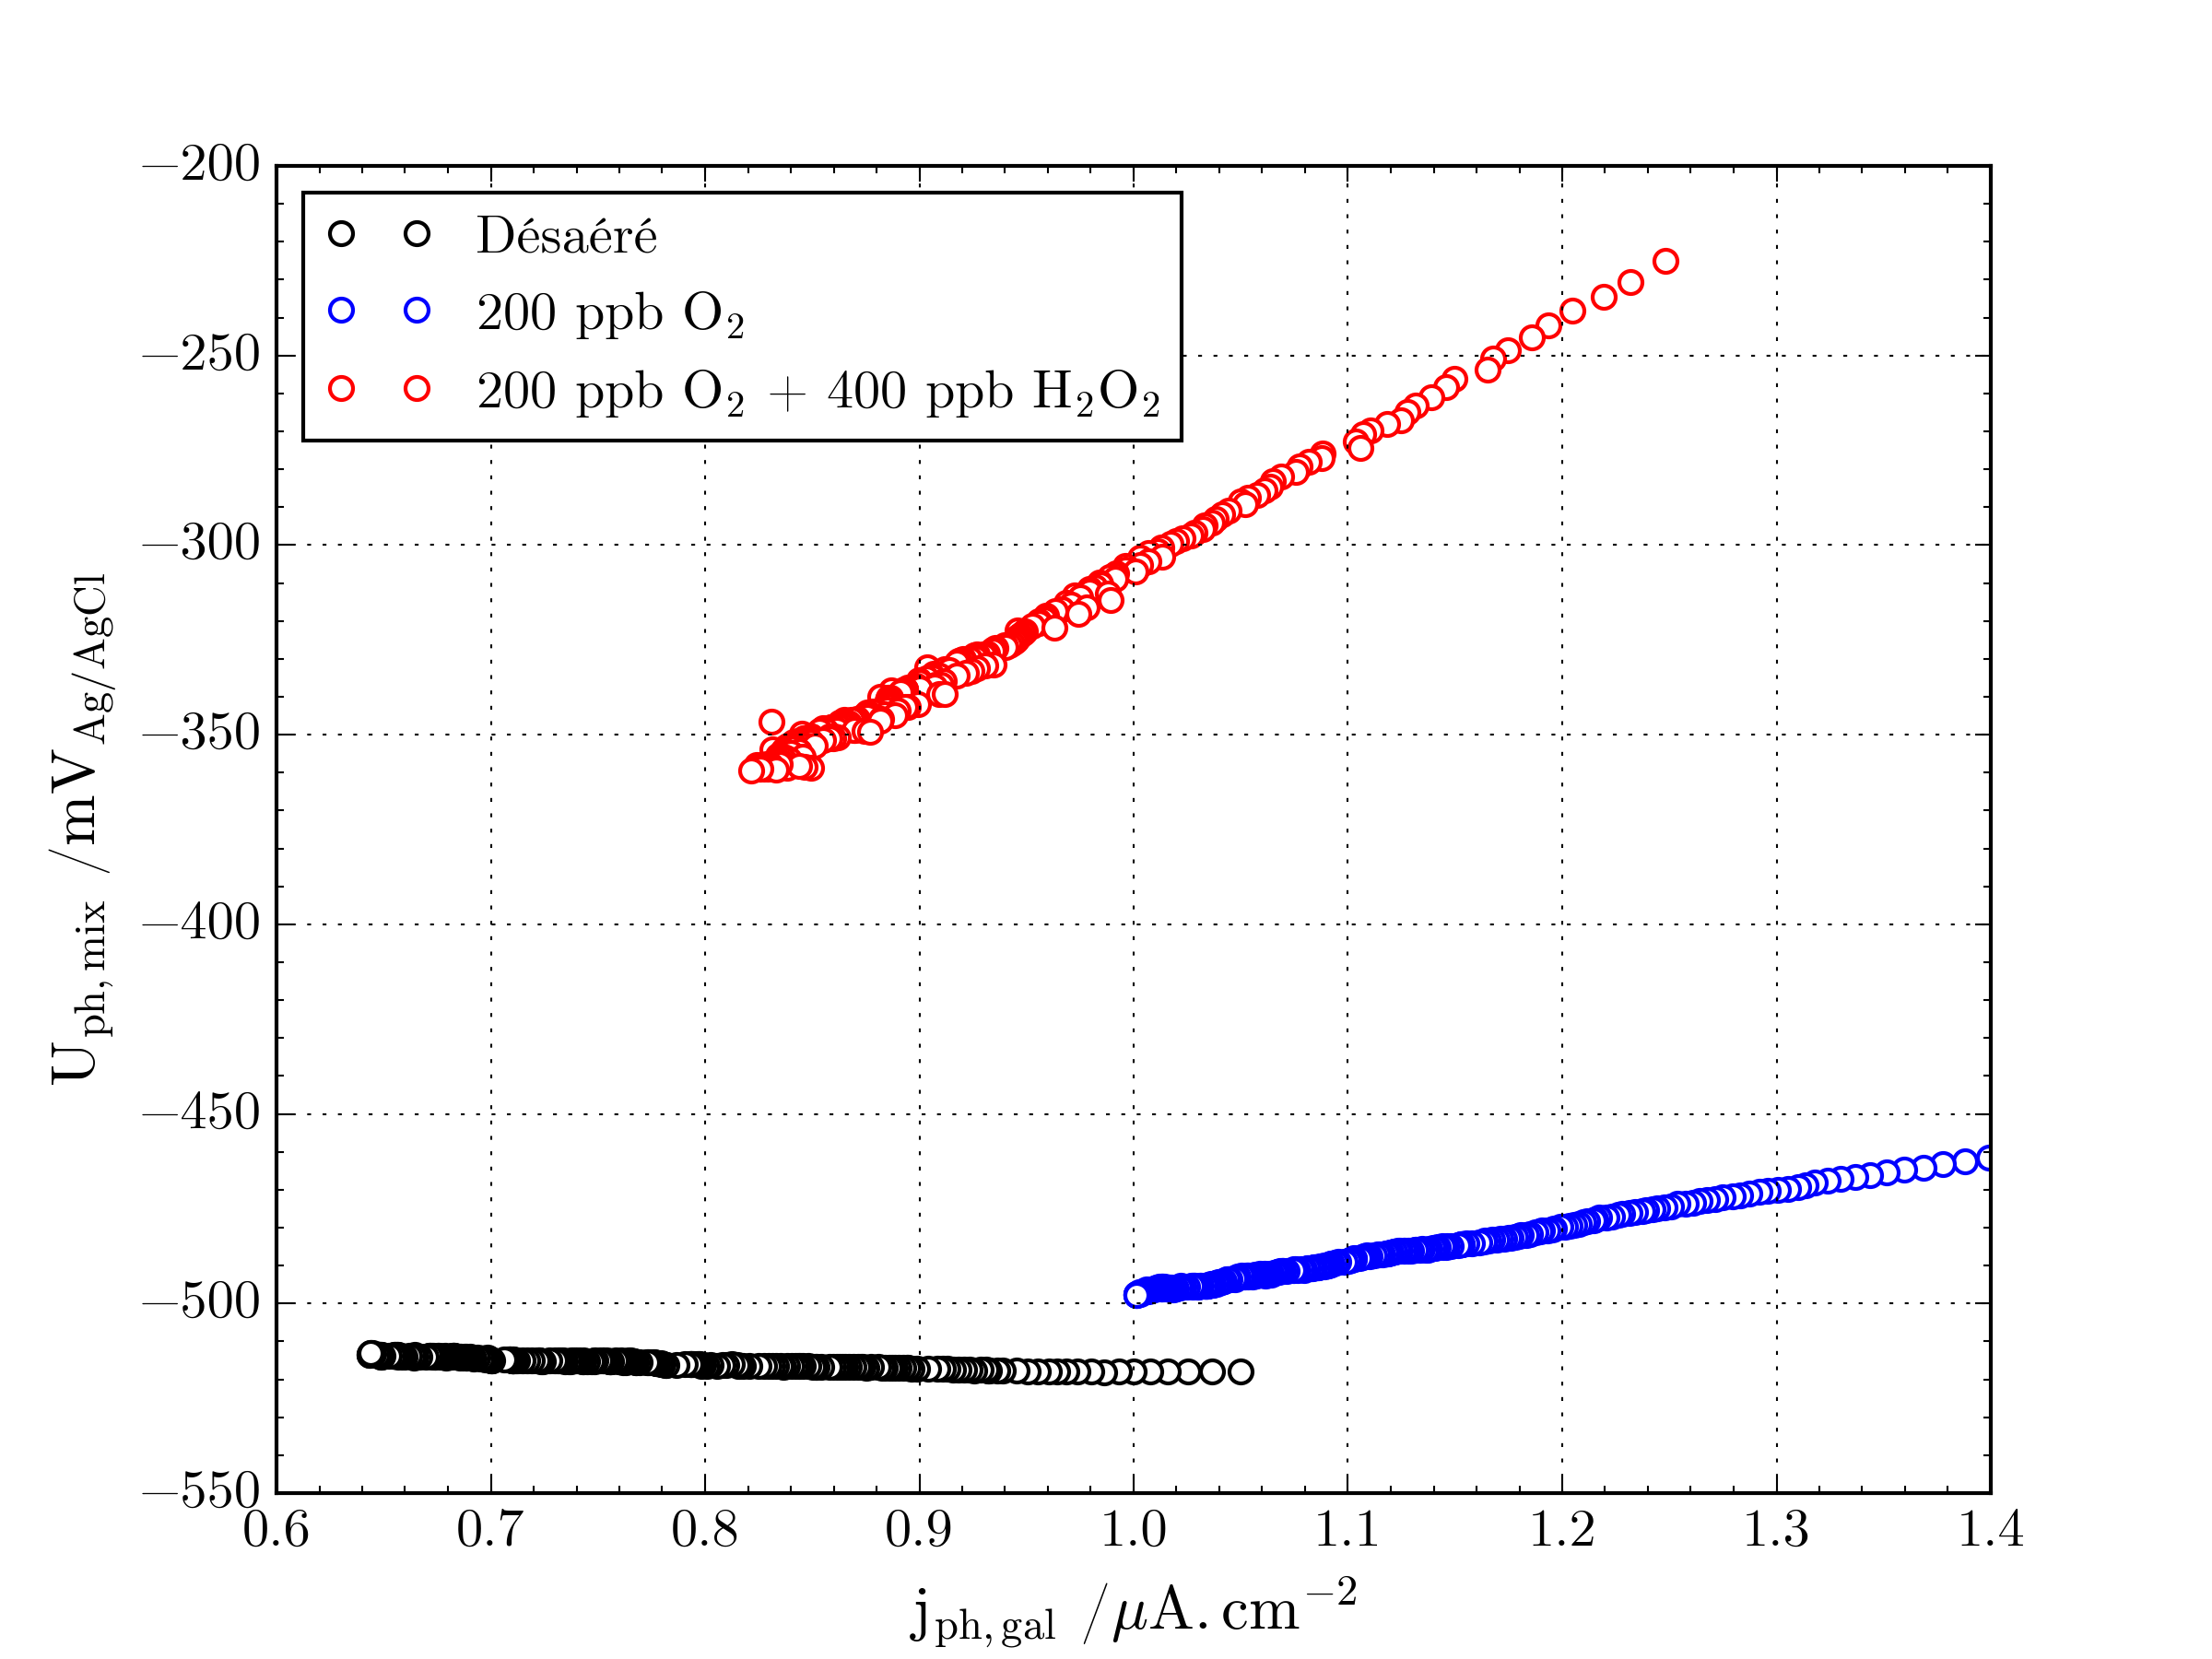
\includegraphics[width=\figwidth]{150215-chap4-ZRA-Umix_vs_Igal.png}
        \caption{Evolution du potentiel mixte en fonction de la densité de courant pendant la première illumination
        UV--Visible pour les trois électrolytes considérés.}
        \label{fig:ch4_Umix_vs_jgal}
    \end{figure}

    Bien que nous ne sachions pas encore expliquer l’origine de cette linéarité, cette dernière nous a incité
    à considérer la décroissance concomitante du courant et du potentiel avec le temps, lors de l'illumination, 
    comme pouvant être une conséquence liée à la
    diffusion des espèces redox du volume de l’électrolyte vers la surface de l’échantillon, régie par l’équation de
    Cottrell dont la forme intégrée est donnée par l’équation \ref{eq:ch4_Q_vs_t}. Cette relation lie la charge échangée, Q, avec le
    nombre d’électrons échangés, n, la constante de Faraday, F, la surface exposée, S, la concentration de l’espèce
    oxydante, C, et le temps, t.

    \begin{equation}
        Q = 2nFSC\sqrt{\frac{Dt}{\pi}}
        \label{eq:ch4_Q_vs_t}
    \end{equation}

    La figure \ref{fig:ch4_Q_UV} illustre l’évolution de la charge Q en fonction de $\sqrt{t}$ pour les trois électrolytes considérés.
    La relation
    de linéarité observée semble indiquer que l’électrolyte contenant 200~ppb d’oxygène dissous, sans peroxyde d’hydrogène,
    permet d’échanger la plus grande charge électrique. Il apparaît également que la présence d’oxygène et de peroxyde
    d’hydrogène induit une charge supplémentaire plus faible par rapport à l’électrolyte constitué d’eau ultra pure désaérée
    à l’argon. Ce résultat nous paraît intéressant car il semble indiquer un potentiel effet de la vitesse d’écoulement de
    l’électrolyte dont la vitesse peut atteindre quelques mètres par seconde en réacteur alors que le débit
    d’écoulement dans la cellule HTP a été fixée à \SI{1}{\milli\liter\per\minute} 
    (c’est-à-dire une vitesse d’écoulement moyenne de \SI{1.5}{\milli\meter\per\second})
    pour y minimiser les problèmes de gestion de la température (chapitre \ref{chap:design}, \S \ref{sec:complete_experimental_setup}). 

    \begin{figure}[H]
        \centering
        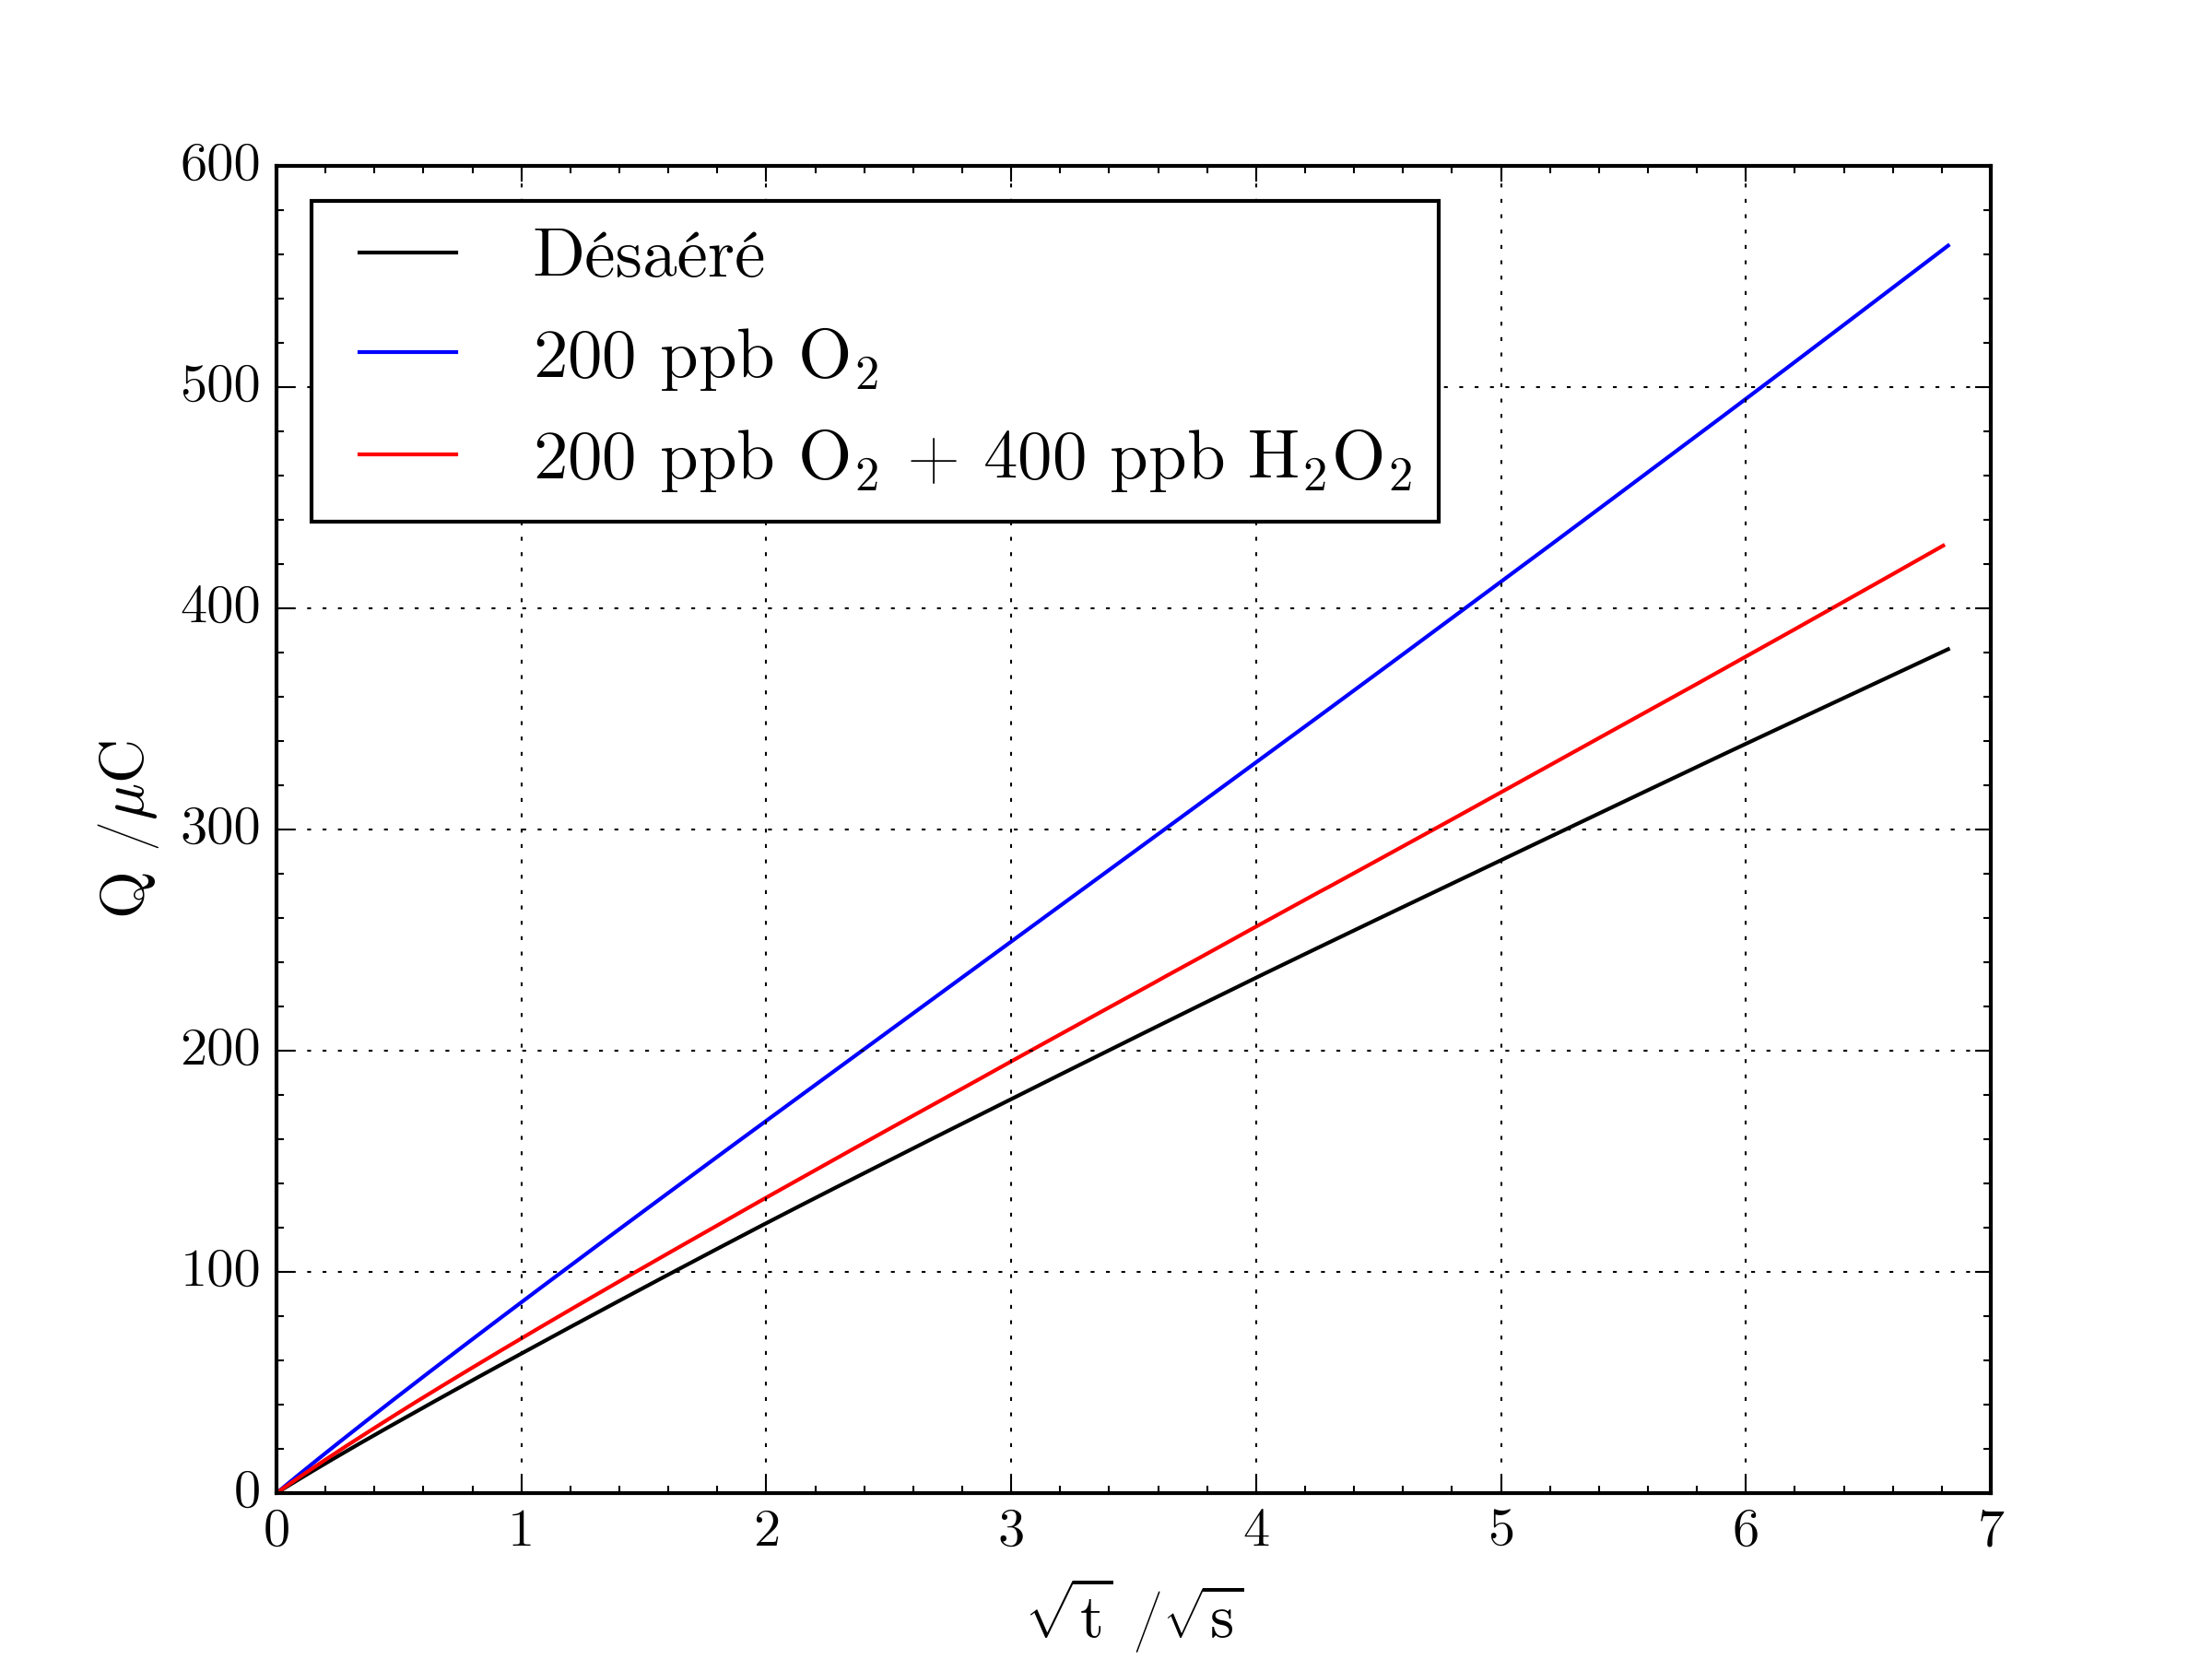
\includegraphics[width=\figwidth]{150215-chap4-ZRA-Q_vs_time.png}
        \caption{Evolution de la charge électrique (obtenue par intégration du courant de couplage de la figure \ref{fig:ch4_ZRA_UV_ON_OFF})
        pendant la première illumination UV--Visible pour les trois électrolytes considérés.}
        \label{fig:ch4_Q_UV}
    \end{figure}

    Par ailleurs, on peut également noter que les valeurs de densité de courant obtenues ici sont du même ordre de grandeur
    que celles classiquement observées lors d’essais d’oxydation en autoclave avec et sans illumination (chapitre
    \ref{chap:ch1_bib}, figure \ref{fig:ch1_Zy2_Kinetics_th_J}).
    Bien que les courants de couplages mesurés dans nos conditions n’atteignent pas les ordres de grandeur de densités
    de courant correspondant au phénomène de Shadow Corrosion 
    (environ \SI{10}{\micro\ampere\per\square\centi\meter}, chapitre \ref{chap:ch1_bib}, figure \ref{fig:KKL_shadow_digitalization}), nos résultats
    montrent tout de même que la seule illumination UV--Visible augmente les courants de couplage, et donc potentiellement la
    corrosion du Zy2. La différence entre les ordres de grandeur des courants de couplage dans nos conditions et dans les
    conditions réelles de la Shadow Corrosion est à notre avis liée à l’existence, en conditions réelles de REB,
    du rayonnement neutronique et/ou du rayonnement $\gamma$, absent dans nos conditions expérimentales, rayonnements qui très
    probablement impactent la conduction ionique dans la couche de zircone (chapitre \ref{chap:ch1_bib}, figures \ref{fig:Bererd_diffusion_increase}
    et \ref{fig:irradiation_effect_IE_plots}).

    En outre, en réacteur réel, le flux de rayonnement UV (rayonnement de Cherenkov) induit par ces rayonnements
    neutroniques et $\gamma$ est très certainement bien plus important que le flux lumineux disponible dans nos expériences.  Nous
    avons tenté de déterminer quel flux lumineux UV--Visible aurait été nécessaire dans nos conditions expérimentales (avec
    la lampe Hg) pour obtenir les ordres de grandeur de courant de couplage observés en Shadow Corrosion. Pour cela, nous
    avons réalisé des mesures de courant de couplage en modifiant le niveau de puissance à la sortie de la lampe Hg , donc
    en modifiant le flux lumineux arrivant sur l’échantillon. 

    La figure \ref{fig:ch4_Iph_vs_Power} illustre les résultats de ces expériences pour le cas de l’électrolyte contenant de l’oxygène dissous à
    une teneur de 200~ppb. La grandeur portée en ordonnée est le rapport entre la densité de courant de couplage mesurée
    sous illumination et celle mesurée à l’obscurité (juste avant illumination). La grandeur portée en abscisse est la
    puissance lumineuse (polychromatique) totale en sortie de lampe, calculée en multipliant la puissance de sortie maximale
    de la lampe Hg sur l’ensemble du spectre d’émission (chapitre \ref{chap:design}, figure \ref{sec:ch3_UV_sources}), soit
    \SI{40}{\watt\per\square\centi\meter}, par le niveau de puissance
    (5\%, 20\%, 50\% ou 100\%). La puissance calculée de cette manière ne correspond pas réellement à celle reçue par
    l’échantillon en cellule HTP, mais nous pouvons la considérer comme une bonne homothétie de la
    réalité. 

    \begin{figure}[H]
        \centering
        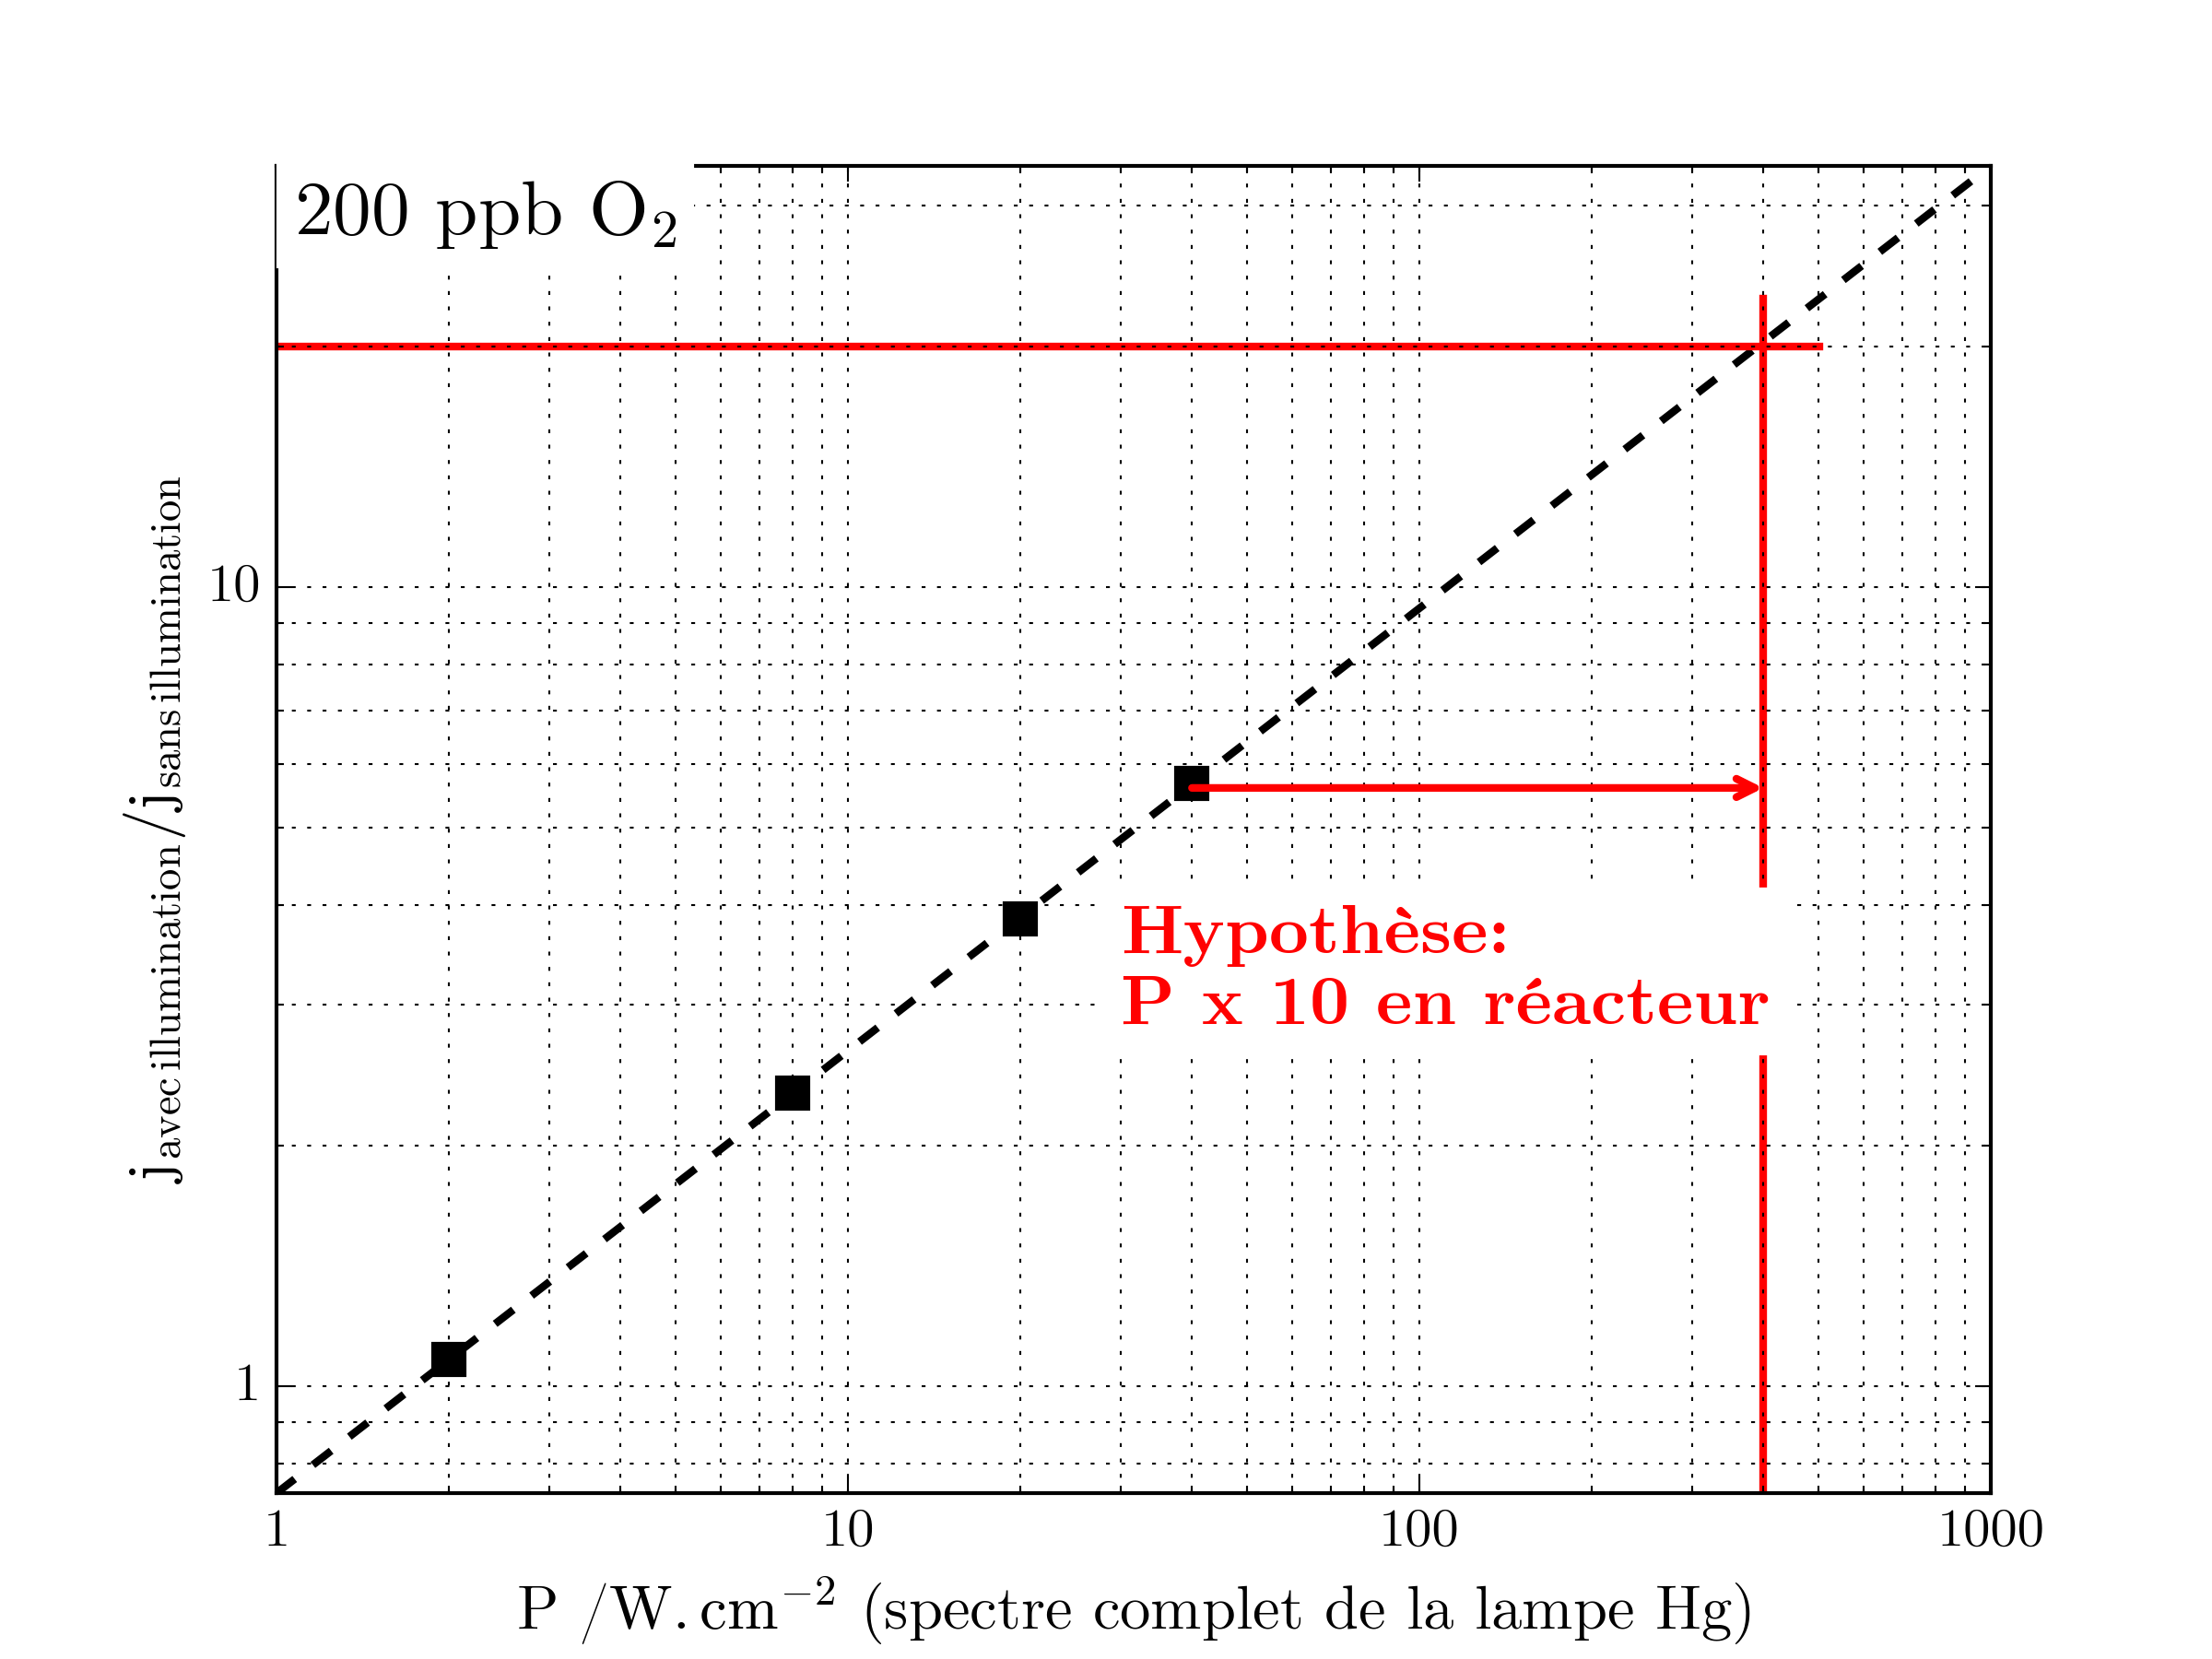
\includegraphics[width=\figwidth]{150215-chap4-ZRA-Igal_vs_Flux-Px10.png}
        \caption{Evolution du rapport entre les densités de courant de couplage avec et sans illumination UV--Visible et
        la puissance d’illumination UV--Visible, pour le cas de l’électrolyte présentant une teneur en oxygène dissous de
    200~ppb.}
        \label{fig:ch4_Iph_vs_Power}
    \end{figure}

    La figure \ref{fig:ch4_Iph_vs_Power} montre une proportionnalité dans l’échelle log--log avec une pente de 0.55 (très proche d’une
    évolution en racine carrée) entre le rapport des densités de courant de couplage avec et sans illumination et la
    puissance lumineuse utilisée. En faisant l’hypothèse que cette proportionnalité reste valide au moins jusqu’à
    10x\SI{40}{\watt\per\square\centi\meter},
    ce que nous ne pouvons cependant pas vérifier, la densité de courant de couplage serait multipliée par vingt
    et atteindrait des valeurs proches de celles observées en Shadow Corrosion.

    Il nous semble que ce protocole de mesures de densités de courant de couplage en fonction de la puissance d’un flux
    lumineux UV--Visible pourrait être mis à profit pour tester de manière relativement rapide en laboratoire diverses
    solutions d’atténuation du phénomène de Shadow Corrosion. Cela permettrait par exemple de tester la susceptibilité
    au couplage galvanique sous illumination UV--Visible de différents couples de matériaux. Par exemple, cela
    permettrait de tester l’impact de revêtements sur les alliages Zy2 et/ou des alliages base nickel.




    \subsection{Courbes de polarisation}\label{subsec:ch4_oxygen_Tafel}

    La figure \ref{fig:ch4_Zy2_Tafel} (resp. \ref{fig:ch4_718_Tafel}) rassemble les courbes de polarisation anodiques
    (resp. cathodiques) de
    l’échantillon Zy2 (resp. Inc718) mesurées à l’obscurité et sous illumination UV--Visible dans chacun des trois
    électrolytes considérés à différentes teneurs en oxygène. Le Tableau 4.5 compile les valeurs de coefficients de
    transfert et de densités de courant d’échange déterminées par régression linéaire sur les points expérimentaux de
    ces courbes de polarisation.

    Il convient de préciser que les mesures correspondantes ont été réalisées de manière séquentielle, en démarrant avec
    l’électrolyte en condition désaérée, en y introduisant ensuite l’oxygène puis le peroxyde d’hydrogène. La mesure des
    courbes de polarisation étant loin d’être instantanée, les échantillons testés se passivent d’une courbe de polarisation
    à la suivante, et les valeurs des densités de courant mesurées diminuent globalement entre les expériences menées en
    condition désaérée et celles correspondant à des teneurs de 200~ppb d’oxygène et de 400~ppb de peroxyde d’hydrogène
    dissous. Aussi nous ne nous intéresserons principalement qu’à la comparaison des valeurs de coefficients de transfert et
    de densités de courant d’échange obtenues avec ou sans illumination UV--Visible, pour chaque électrolyte.

    Préalablement à la discussion des résultats de ces expériences, il nous paraît utile de rappeler quelques notions sur le
    transfert de charge à une interface entre un électrolyte et un semiconducteur idéal, en termes de coefficients de
    transfert et de densité de courant d’échange. Au chapitre \ref{chap:ch1_bib} (\S
    \ref{subsec:semiconductor_electrolyte_contact_light},
    figure \ref{fig:ch1_photocurrent_examples}), nous avons vu qu’un
    photocourant anodique significatif apparaît sous illumination pour les semiconducteurs de type \emph{n}, la densité de courant
    pouvant être fortement augmentée. A l’obscurité, les coefficients de transfert cathodique et anodique sont égaux à 1 et
    0, respectivement. Sous illumination, les coefficients de transfert prennent des valeurs intermédiaires, plus ou moins
    proches de 0.5 comme ce qui a été montré par \citet{Bertagna1996}. Cependant, la présence de conduction ionique dans le
    semiconducteur, va imposer les valeurs des coefficients de transfert cathodique entre 0.5 et 1 alors que les valeurs des
    coefficients de transfert anodique prendront des valeurs entre 0 et 0.5 avec ou sans illumination. Autrement dit, si
    l’oxyde étudié est un conducteur mixte, le comportement de type diode de l’interface semiconducteur/électrolyte sera 
    "atténué" par l’existence de la conduction mixte \citep{Gerischer1985}. Cela signifie que les défauts dans l’oxyde peuvent complètement
    contrôler les caractéristiques courant/potentiel \citep{Morrison1980}.

    \begin{table}[H]
        \begin{footnotesize}
        \centering
        \begin{tabular}{p{0.28\textwidth}|%
                        >{\centering\arraybackslash}p{0.14\textwidth}%
                        >{\centering\arraybackslash}p{0.14\textwidth}|%
                        >{\centering\arraybackslash}p{0.14\textwidth}%
                        >{\centering\arraybackslash}p{0.14\textwidth}}
        \toprule
        & \multicolumn{2}{c|}{Inc718} &  \multicolumn{2}{c}{Zy2} \\
        & $\alpha_c$ & $j_0$ /\si{\nano\ampere\per\square\centi\meter} & $\alpha_a$ & $j_0$
        /\si{\nano\ampere\per\square\centi\meter} \\\midrule
        \rowcolor{lightgray} Désaéré & 0.89 $\pm$ 0.05 & 30 $\pm$ 3 & 0.282 $\pm$ 0.006 & 154 $\pm$ 4  \\
        \rowcolor{lightgray} + Illumination UV--Visible & 0.78 $\pm$ 0.05 & 41 $\pm$ 4 & 0.273 $\pm$ 0.006 & 261 $\pm$ 7  \\\hline

        200~ppb $O_2$ & 0.52 $\pm$ 0.02 & 41 $\pm$ 2 & 0.243 $\pm$ 0.004 & 125 $\pm$ 3  \\
        + Illumination UV--Visible & 0.48 $\pm$ 0.02 & 50 $\pm$ 2 & 0.204 $\pm$ 0.004 & 289 $\pm$ 6  \\\hline


        \rowcolor{lightgray} 200~ppb $O_2$ + 400~ppb $H_2O_2$ & 0.58 $\pm$ 0.09 & 35 $\pm$ 5 & 0.189 $\pm$ 0.003 & 89 $\pm$ 2  \\
        \rowcolor{lightgray} + Illumination UV--Visible & 0.60 $\pm$ 0.08 & 27 $\pm$ 4 & 0.305 $\pm$ 0.004 & 138 $\pm$ 3  \\

        \bottomrule
    \end{tabular}
        \caption{Valeurs des coefficients de transfert et densités de courant d’échange calculées par régression
        linéaire à partir des courbes de polarisation des figures \ref{fig:ch4_Zy2_Tafel} et \ref{fig:ch4_718_Tafel}.}
        \label{tab:ch4_tafel_parameters}
        \end{footnotesize}
    \end{table}

    Dans le cas de l’échantillon d’Inc718, les densités de courant d’échange sont systématiquement du même ordre de grandeur
    pour les trois conditions de chimie avec et sans illumination UV--Visible. Pour ce qui concerne les coefficients de
    transfert, et pour un électrolyte donné, les valeurs déterminées en présence et en l’absence d’illumination sont très
    proches, excepté peut-être pour le cas de l’électrolyte désaéré. Ces valeurs sont autour de 0.5 et 0.6 en présence
    respectivement d’oxygène et de peroxyde d’hydrogène dans l’électrolyte, alors que pour l’électrolyte désaéré, les
    valeurs sont plus proches de 1, ce qui pourrait s’expliquer par le développement de réactions électrochimiques
    d’insertion/désinsertion à l’électrode Inc718 oxydée dans le cas des électrolytes chargés en oxygène. L’alliage de
    nickel X750, préoxydé dans les mêmes conditions que l’échantillon d’Inc718, présente des coefficients de transfert
    similaires en eau ultra-pure avec 200~ppb d’oxygène dissous : $\alpha _c$ vaut 0.47 sans illumination UV--Visible et 0.45 avec
    illumination UV--Visible.

    Dans le cas de l’échantillon Zy2, les coefficients de transfert varient sur une gamme de valeurs restreinte de 0.20 à
    0.28 en condition désaérée et avec 200~ppb d’oxygène, que ce soit à l’obscurité ou sans illumination. Une variation du
    coefficient de transfert entre obscurité et illumination plus nette est observée lorsque l’électrolyte contient 200~ppb
    d’oxygène en combinaison avec 400~ppb de peroxyde d’hydrogène. Cependant, les valeurs restent proches et intermédiaires
    entre 0 et 0.5 suggérant un effet plus important de la conduction ionique des échantillons. Par ailleurs, contrairement
    au cas de l’Inc718, les densités de courant d’échange sont augmentées sous lumière, d’un facteur 1.7, 2.3 et 1.6
    respectivement pour les conditions sans oxygène, avec 200~ppb d’oxygène et avec 200~ppb d’oxygène en combinaison avec
    400~ppb de peroxyde d’hydrogène.


    Ainsi, l’illumination UV--Visible ne semble modifier de manière significative que la densité de courant d’échange de
    l’alliage Zy2, mais sans modifier les coefficients de transfert. Nous pouvons donc raisonnablement proposer que
    l’augmentation du courant de couplage sous illumination observée sur la figure \ref{fig:ch4_ZRA_UV_ON_OFF} traduise
    l’augmentation de la densité
    de courant d’échange.

    On notera que, récemment, \citet{Kim2014} ont testé avec et sans illumination UV--Visible un échantillon de Zy2 préoxydé
    trois mois en eau-ultra pure. Les courbes de polarisation mesurées à \SI{290}{\degreeCelsius} avec 1~ppm d’oxygène puis avec 600~ppb de
    peroxyde d’hydrogène montrent des résultats similaires aux nôtres, c’est-à-dire que seule la densité de courant
    d’échange est affectée par la présence d’illumination UV--Visible.

    \renewcommand{\localfigwidth}{0.5\textwidth}
    \begin{figure}[H]
            \centering
            \begin{subfigure}[b]{\localfigwidth}
                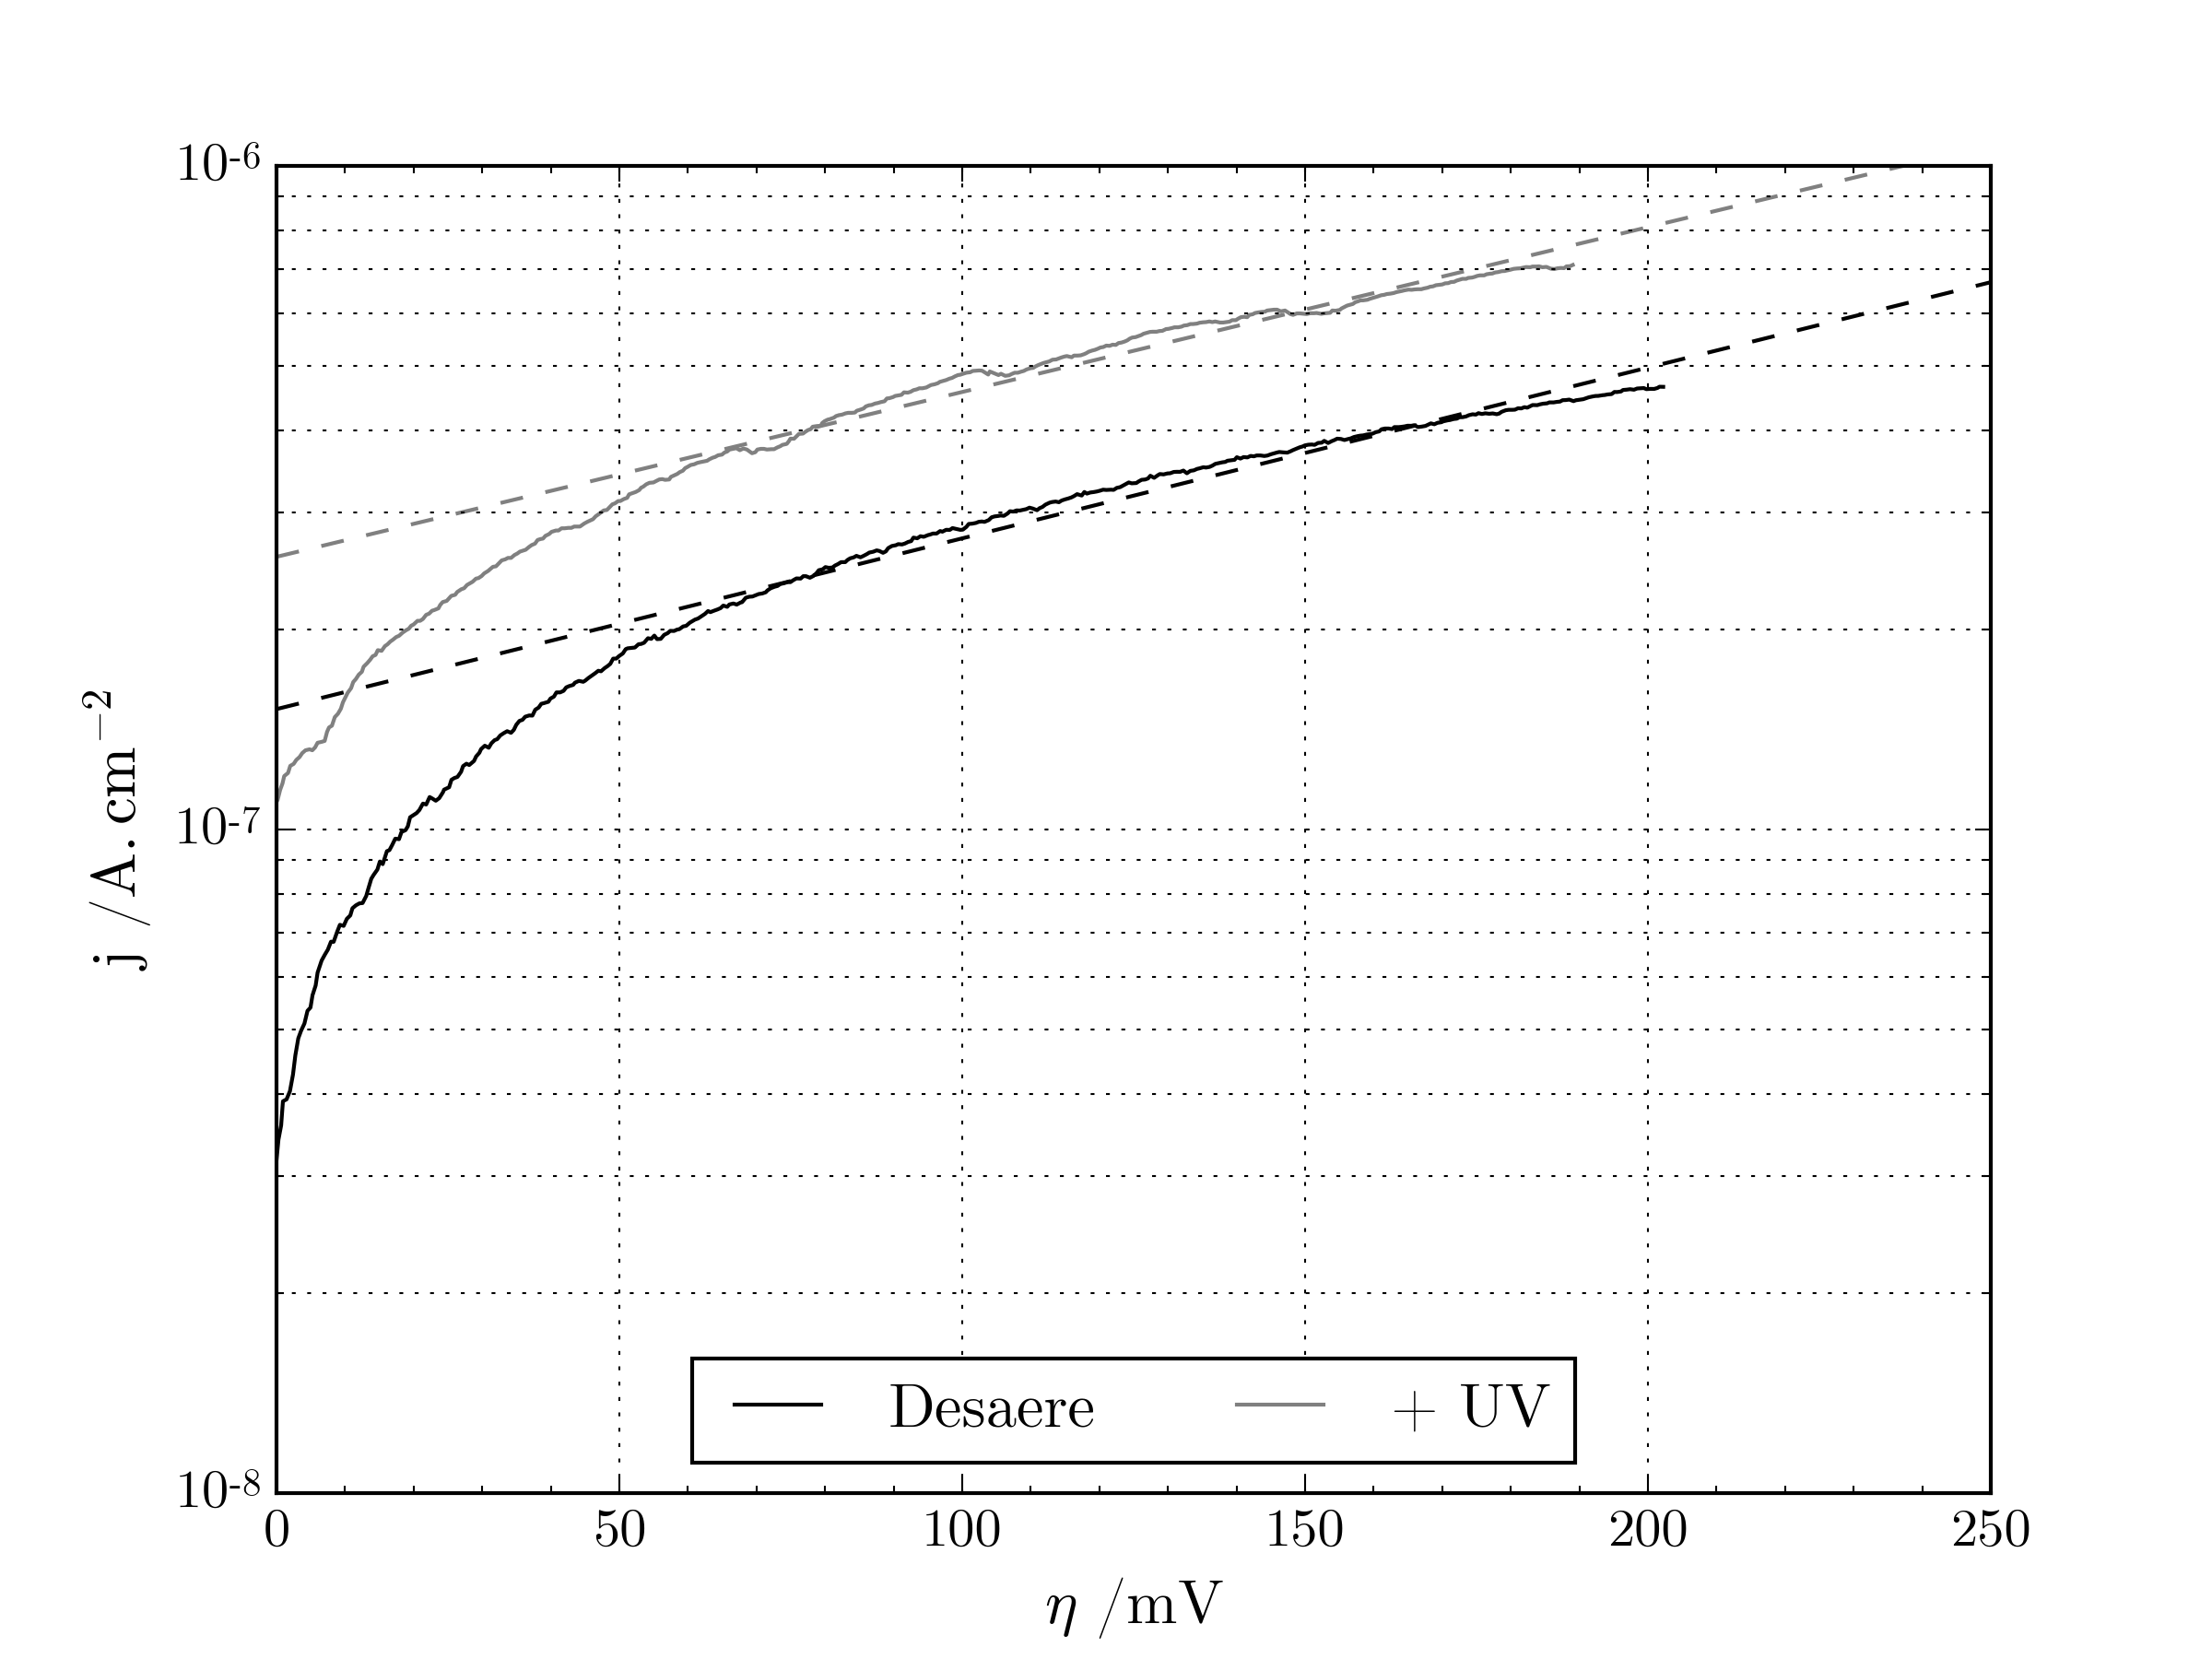
\includegraphics[width=\textwidth]{150215-chap4-PD-Zy2-WE20-n-1.png}
                \caption{}
                \label{}
            \end{subfigure}
            \begin{subfigure}[b]{\localfigwidth}
                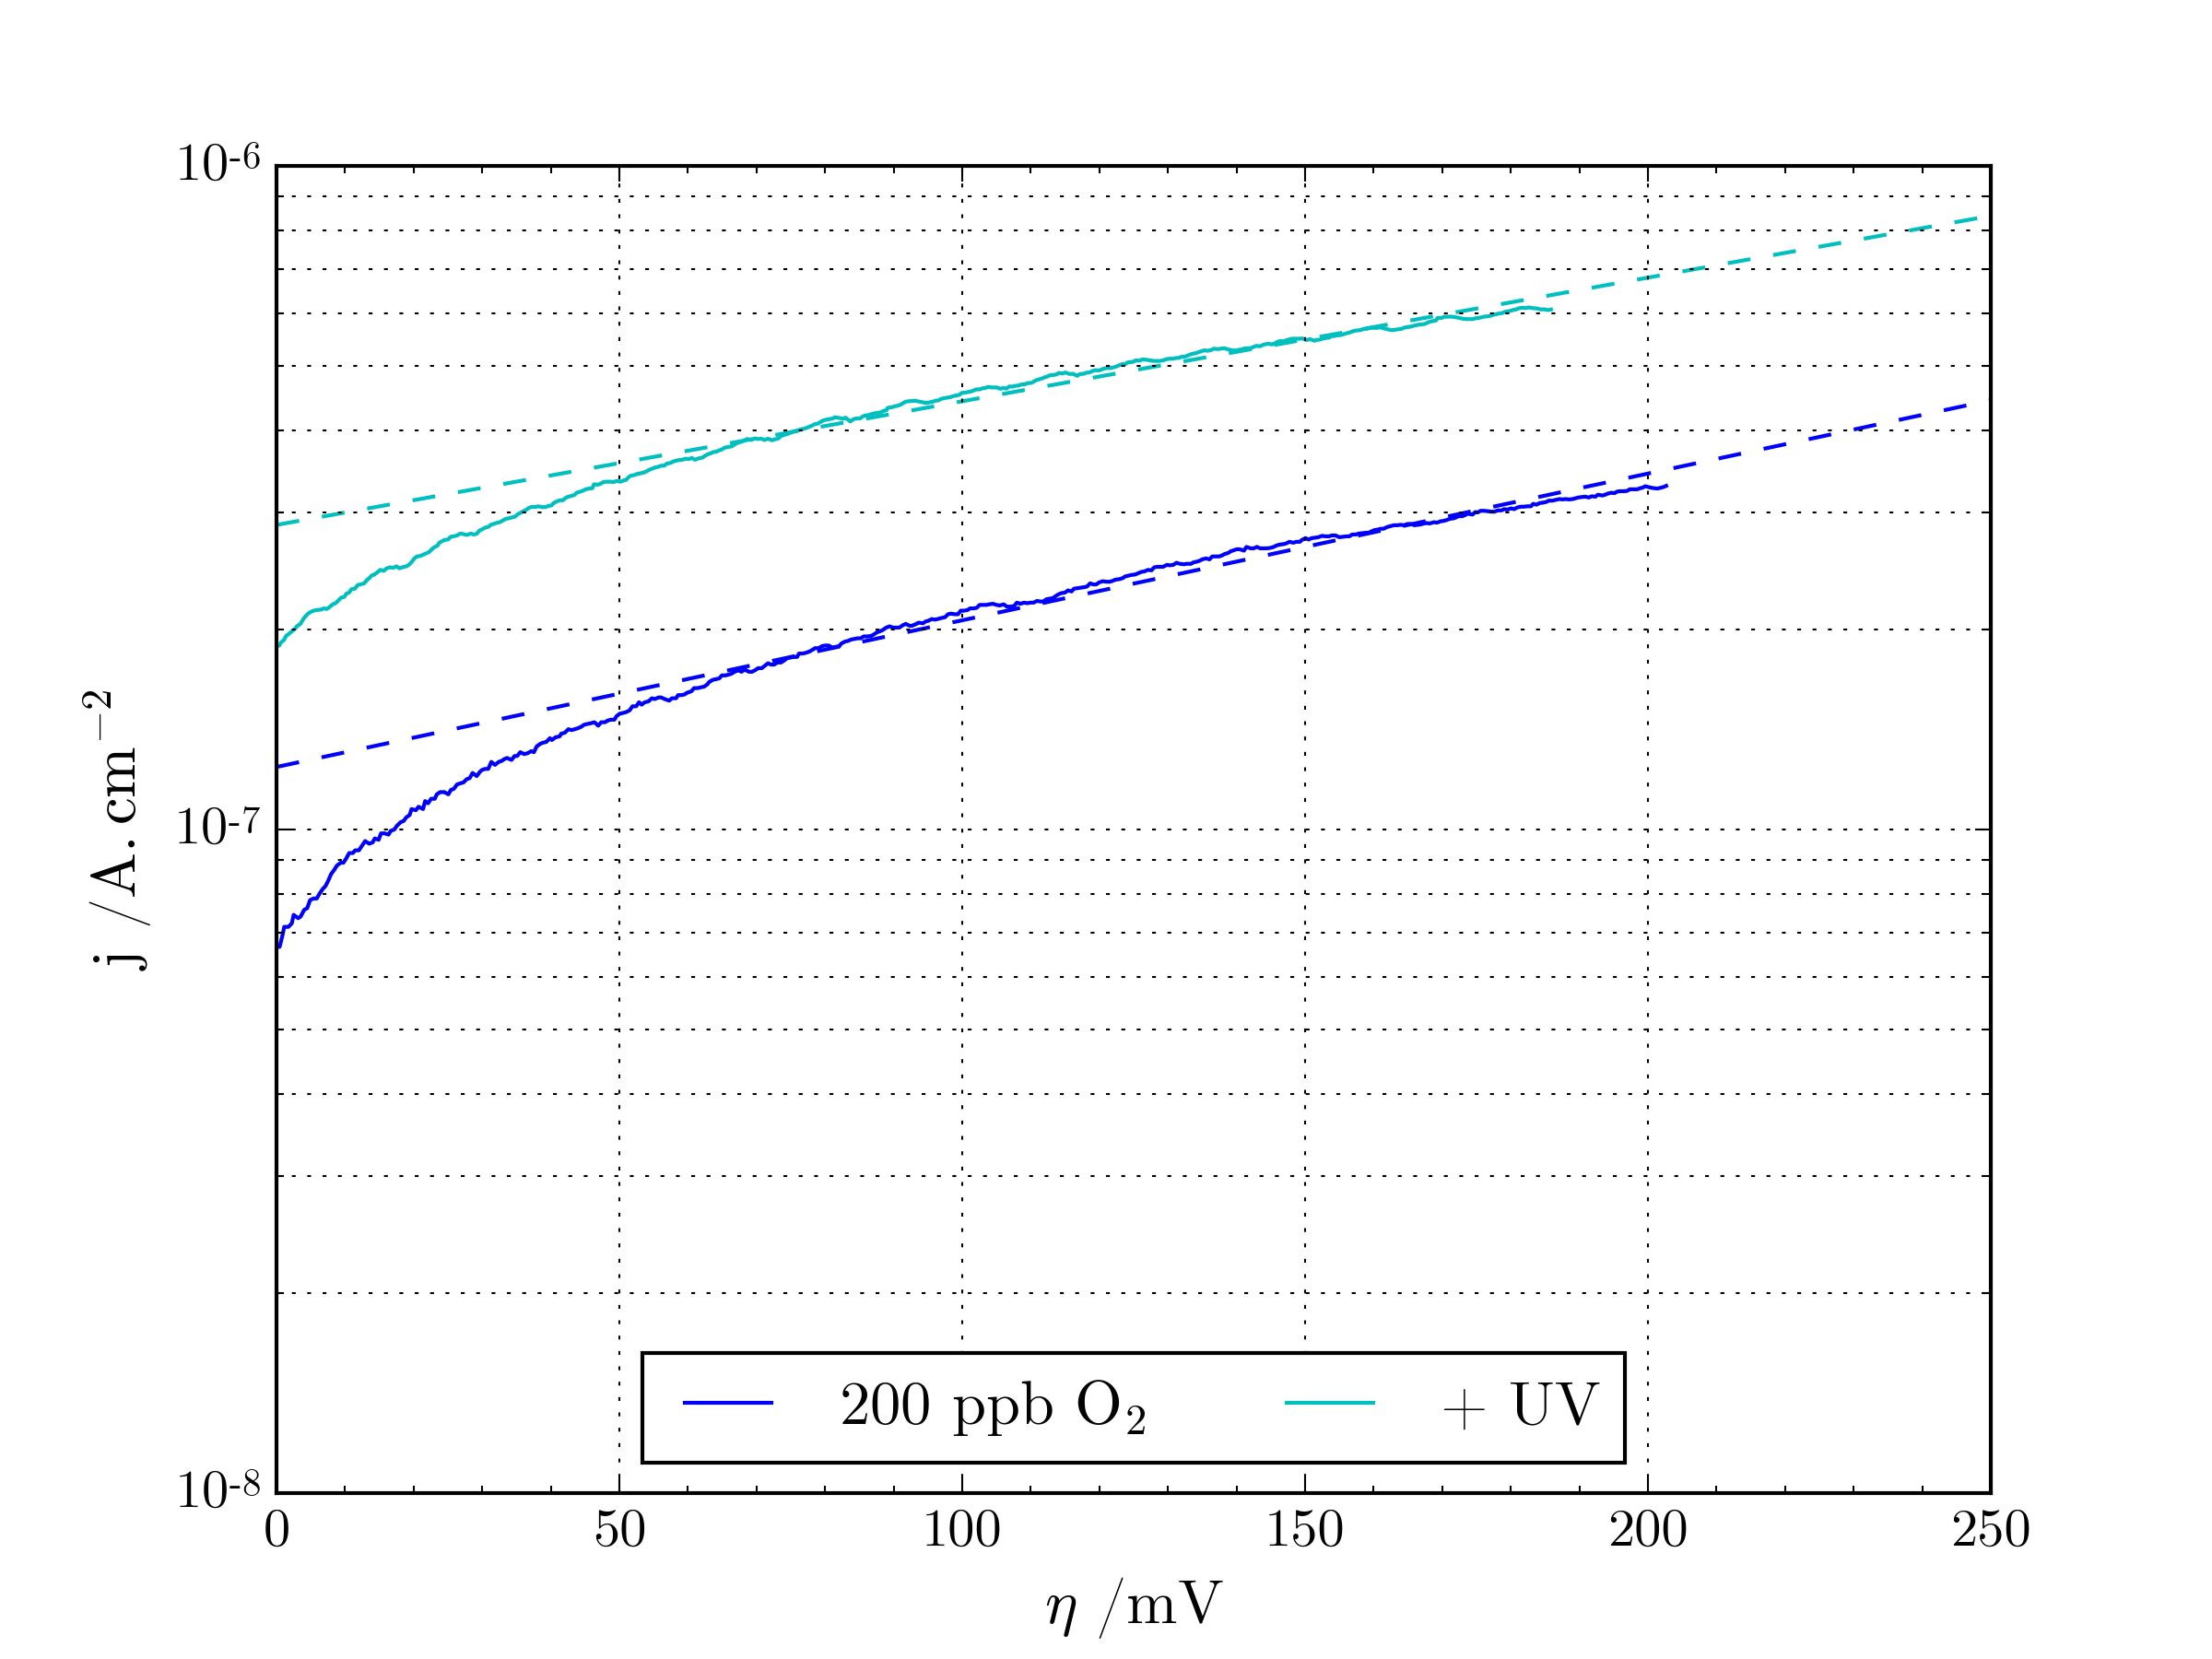
\includegraphics[width=\textwidth]{150215-chap4-PD-Zy2-WE20-n-3.png}
                \caption{}
                \label{}
            \end{subfigure}
            \begin{subfigure}[b]{\localfigwidth}
                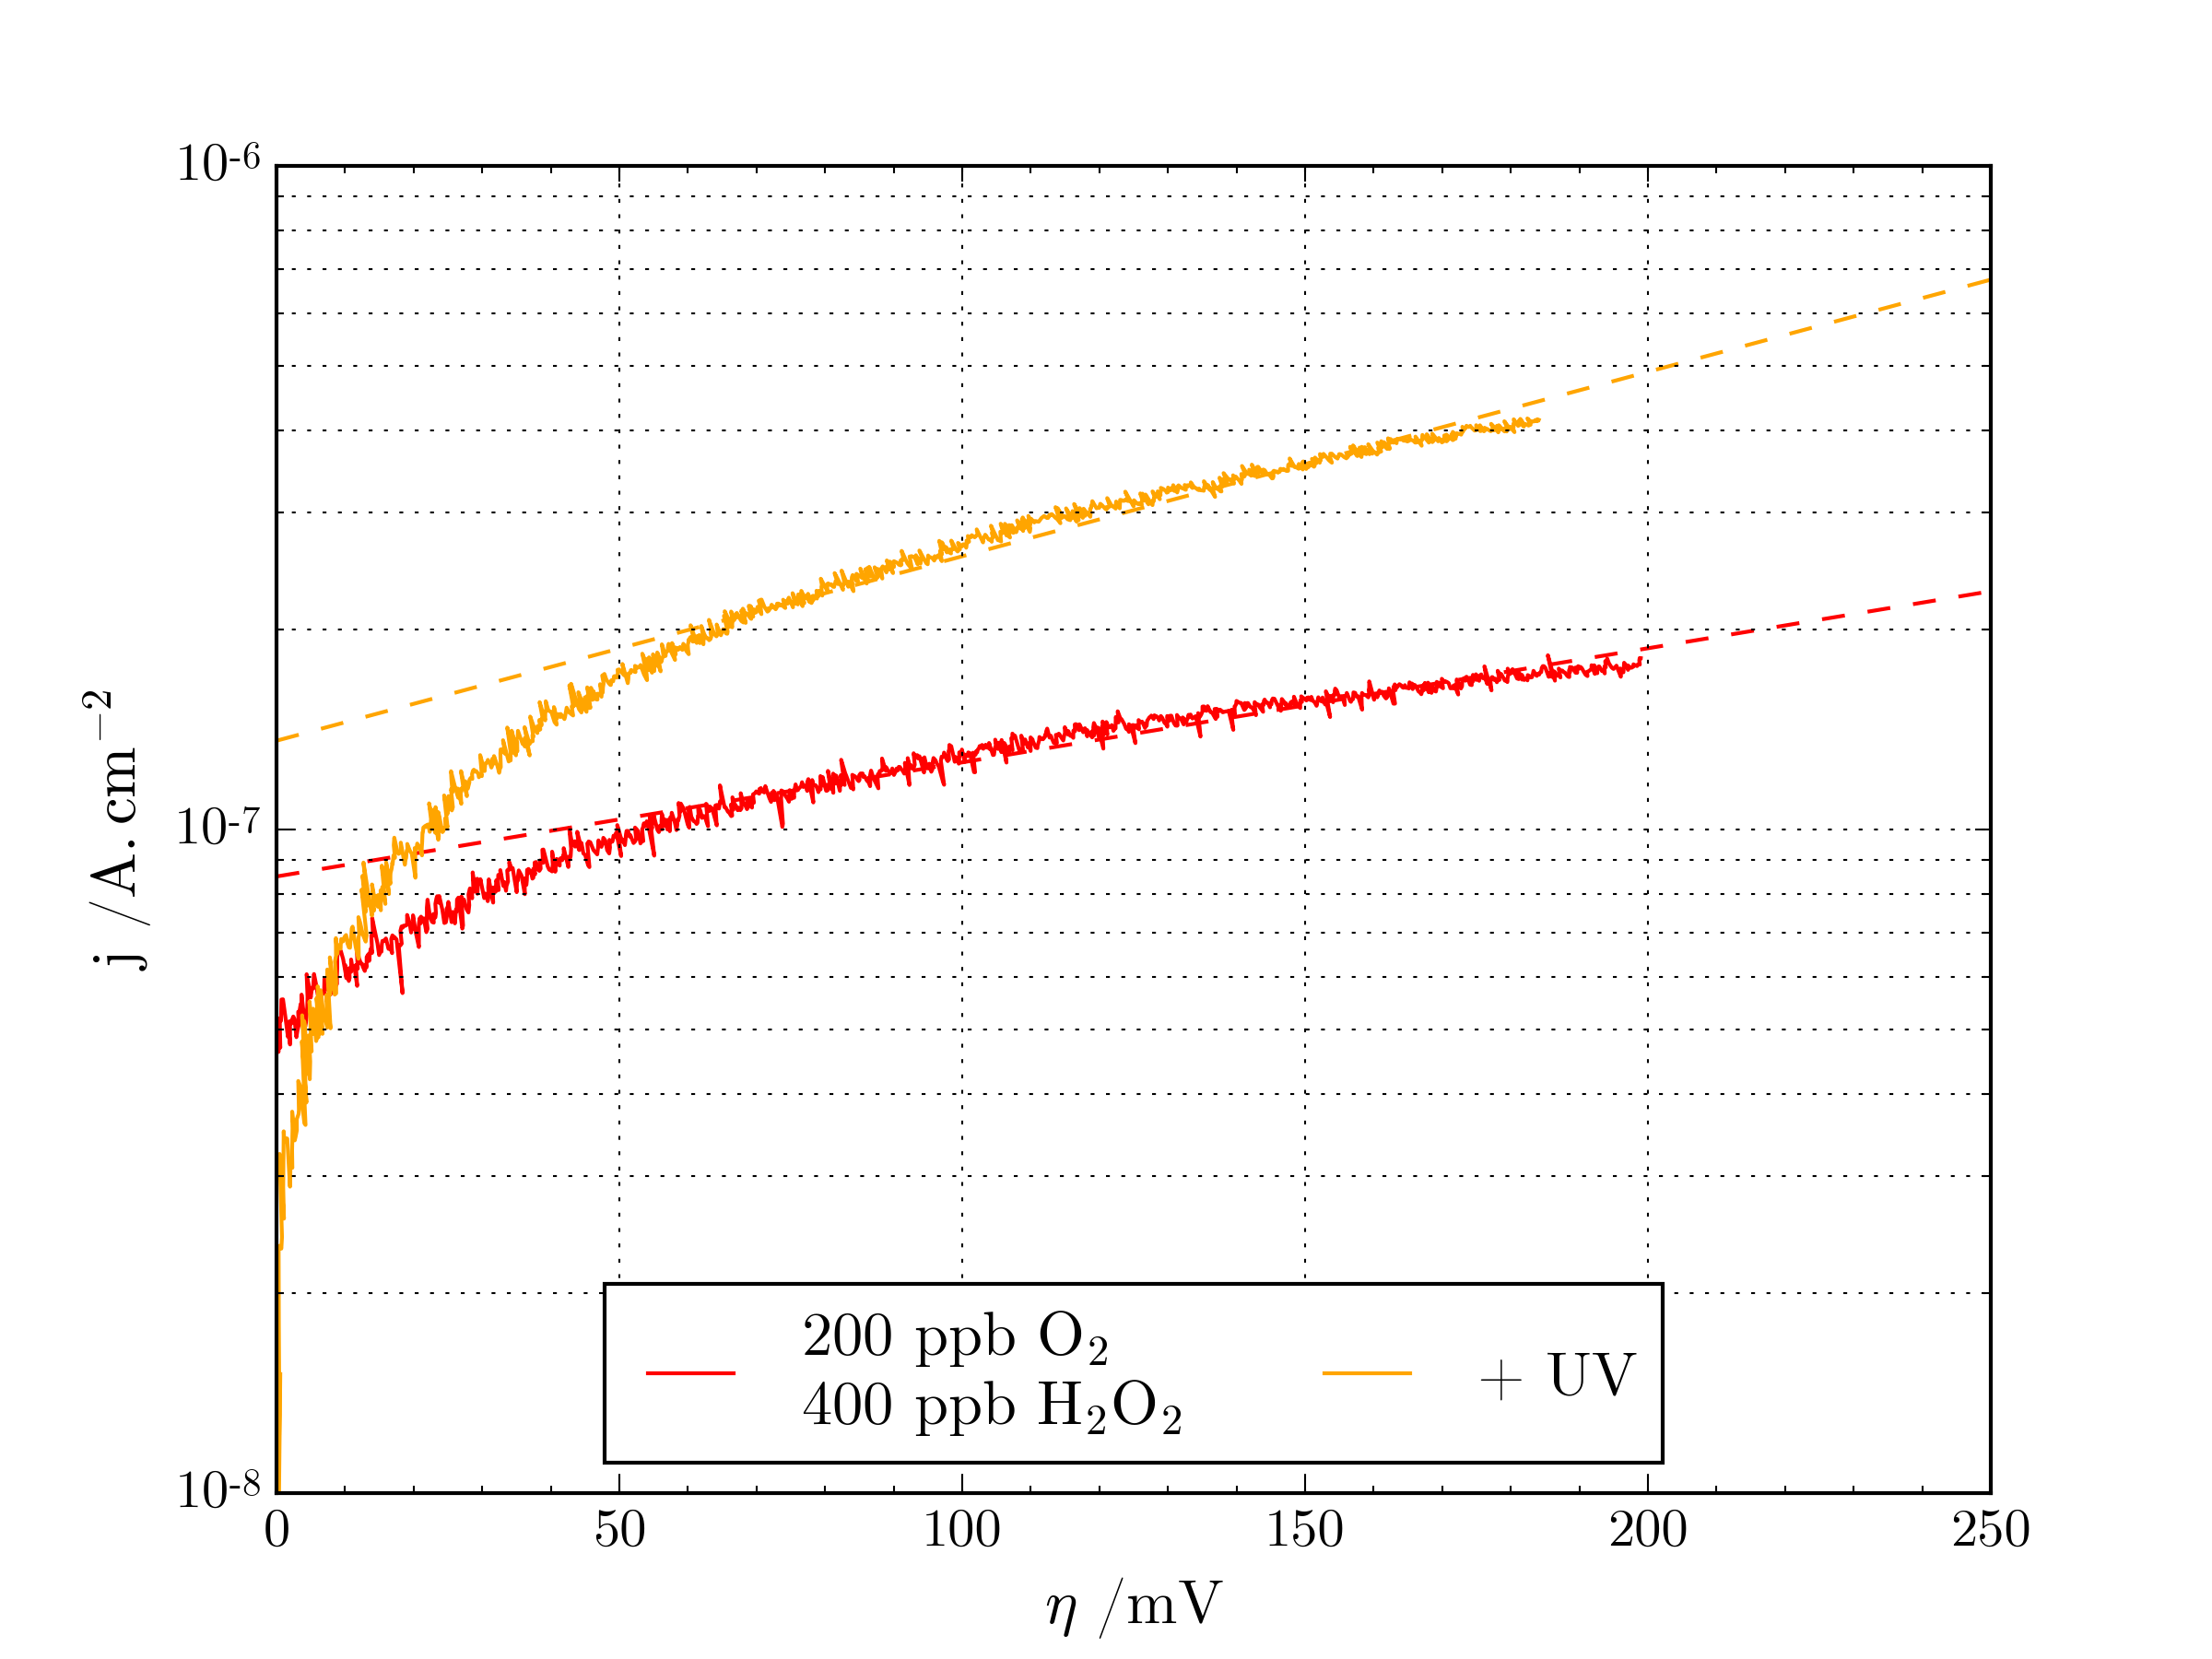
\includegraphics[width=\textwidth]{150215-chap4-PD-Zy2-WE20-n-5.png}
                \caption{}
                \label{}
            \end{subfigure}
            \caption{Evolution des densités de courant anodique de l’échantillon Zy2, avec et sans illumination
            UV--Visible, en fonction de la surtension, pour les trois électrolytes considérés : a) Désaéré, b) 200~ppb
        d’oxygène, c) 200~ppb d’oxygène + 400~ppb de peroxyde d’hydrogène.}
            \label{fig:ch4_Zy2_Tafel}
    \end{figure}

    \begin{figure}[H]
            \centering
            \begin{subfigure}[b]{\localfigwidth}
                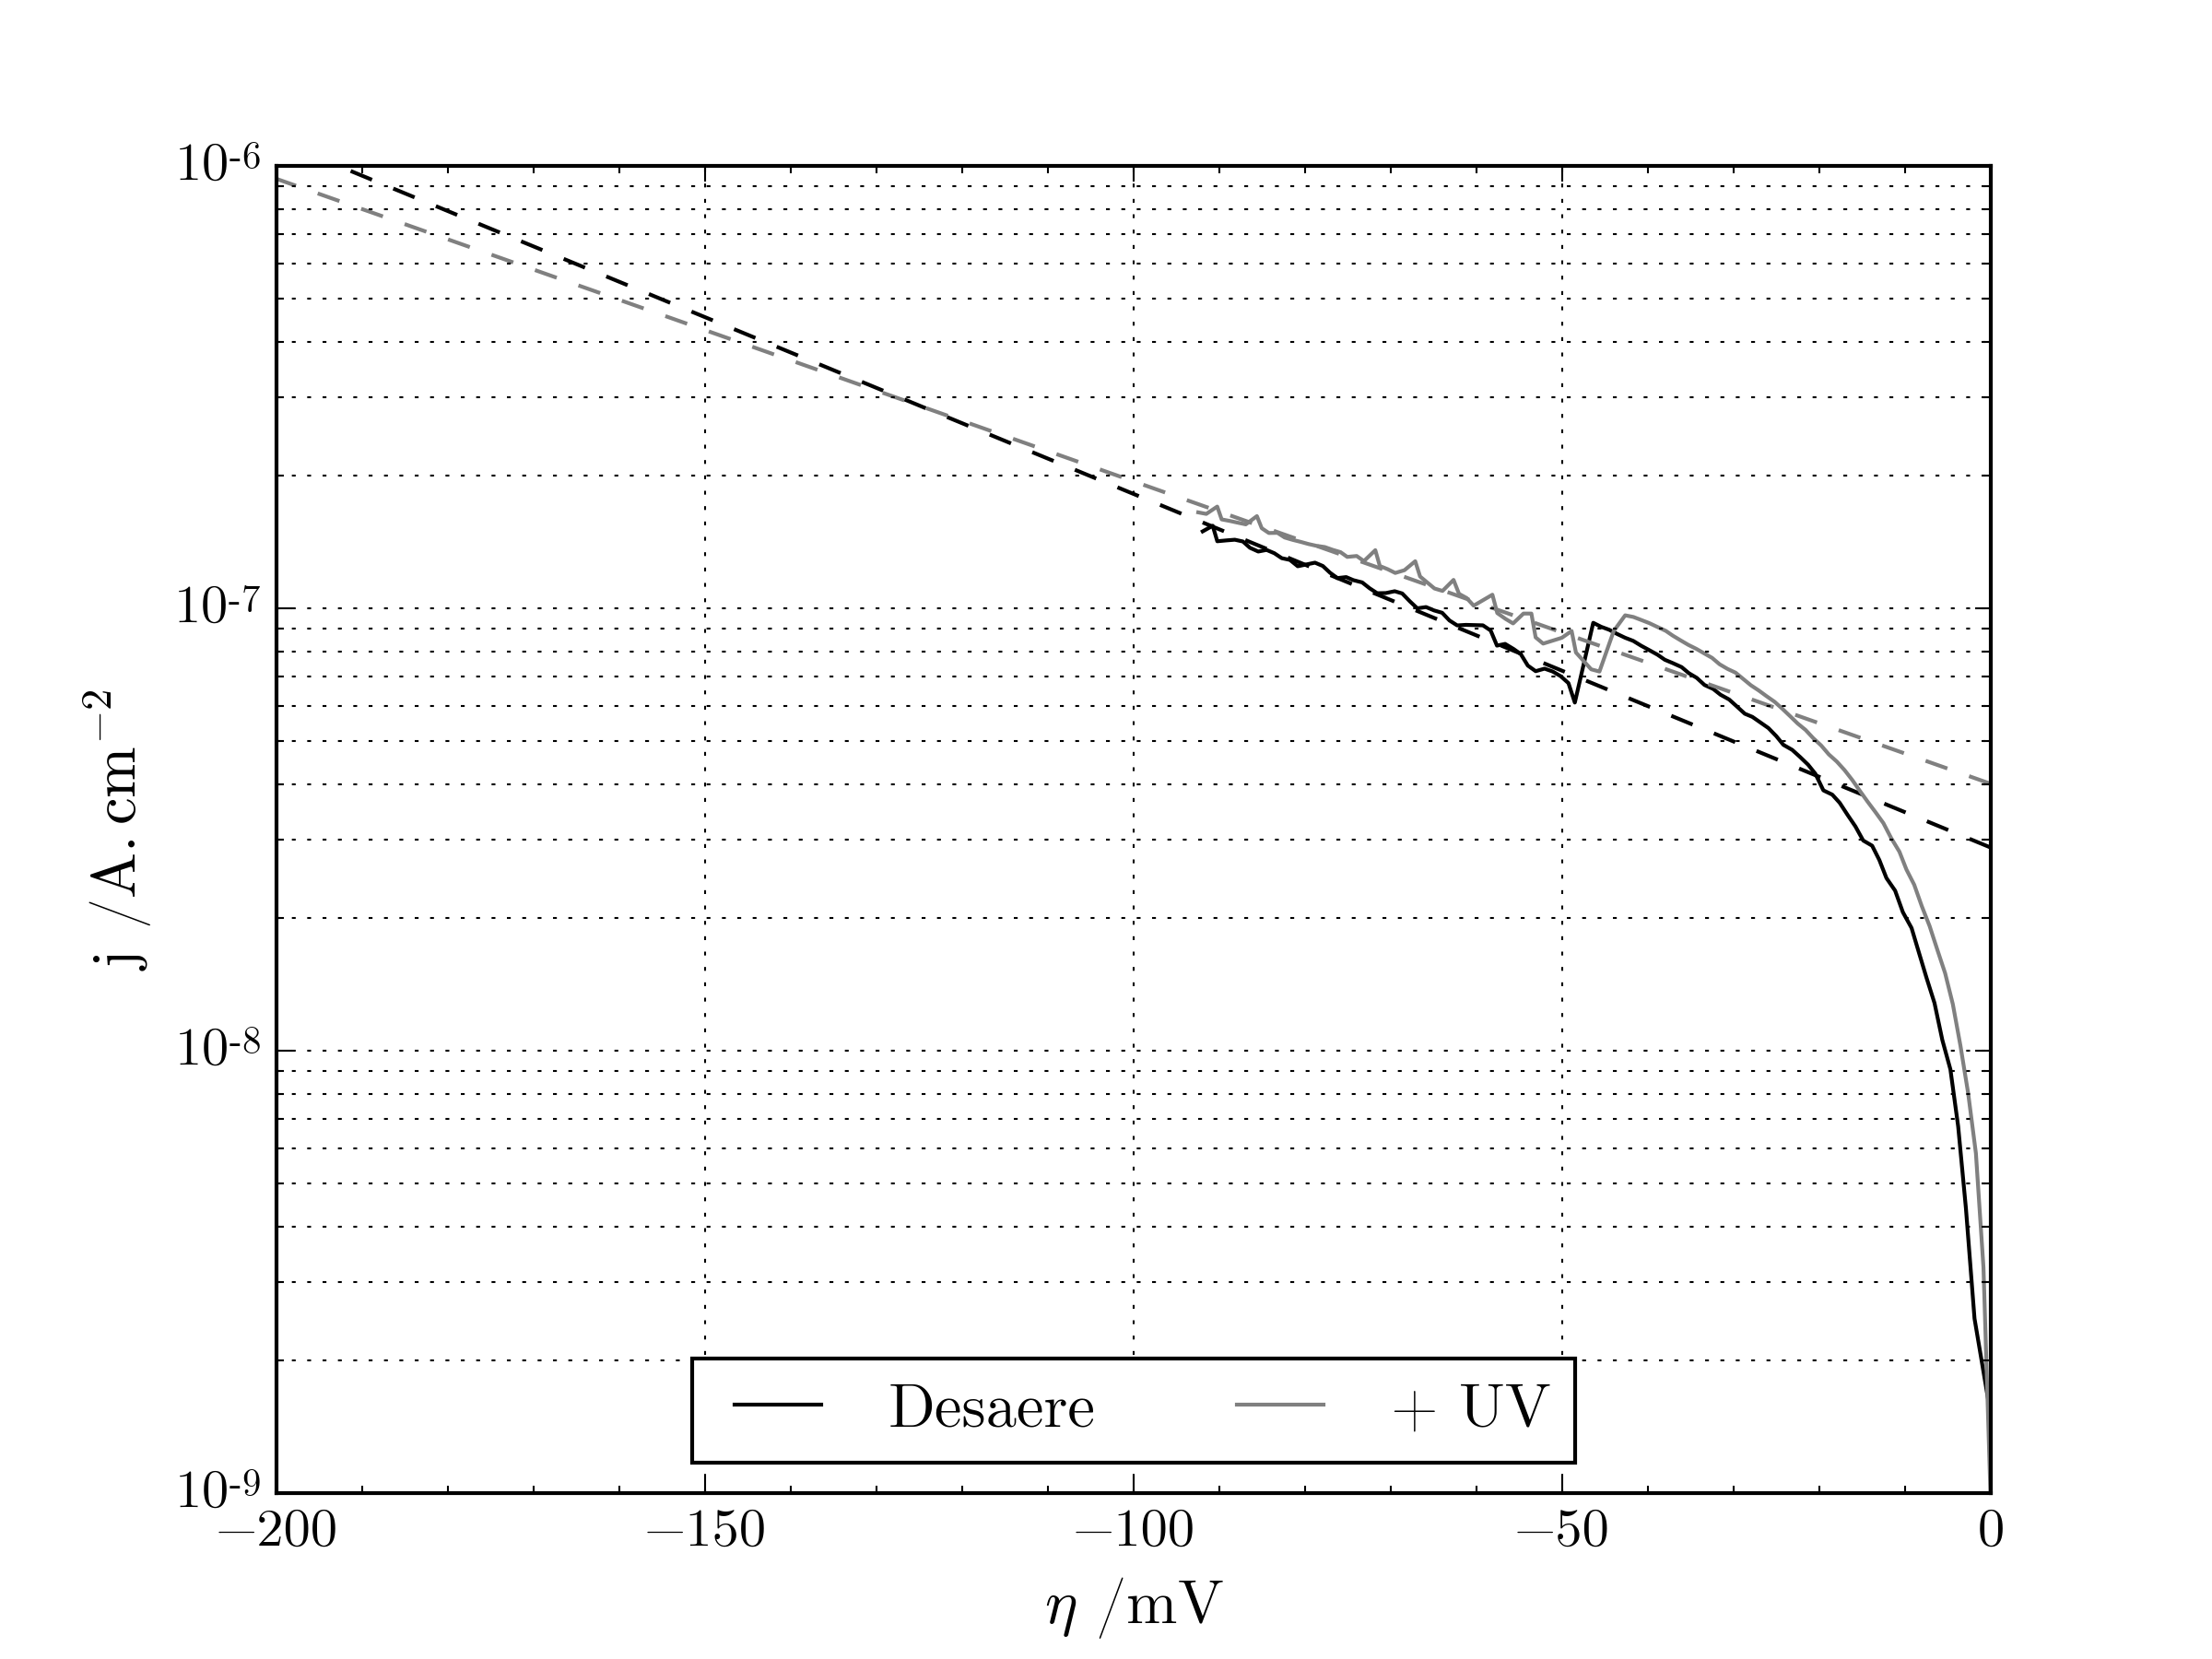
\includegraphics[width=\textwidth]{150215-chap4-PD-Inc718-WE8-n-1.png}
                \caption{}
                \label{}
            \end{subfigure}
            \begin{subfigure}[b]{\localfigwidth}
                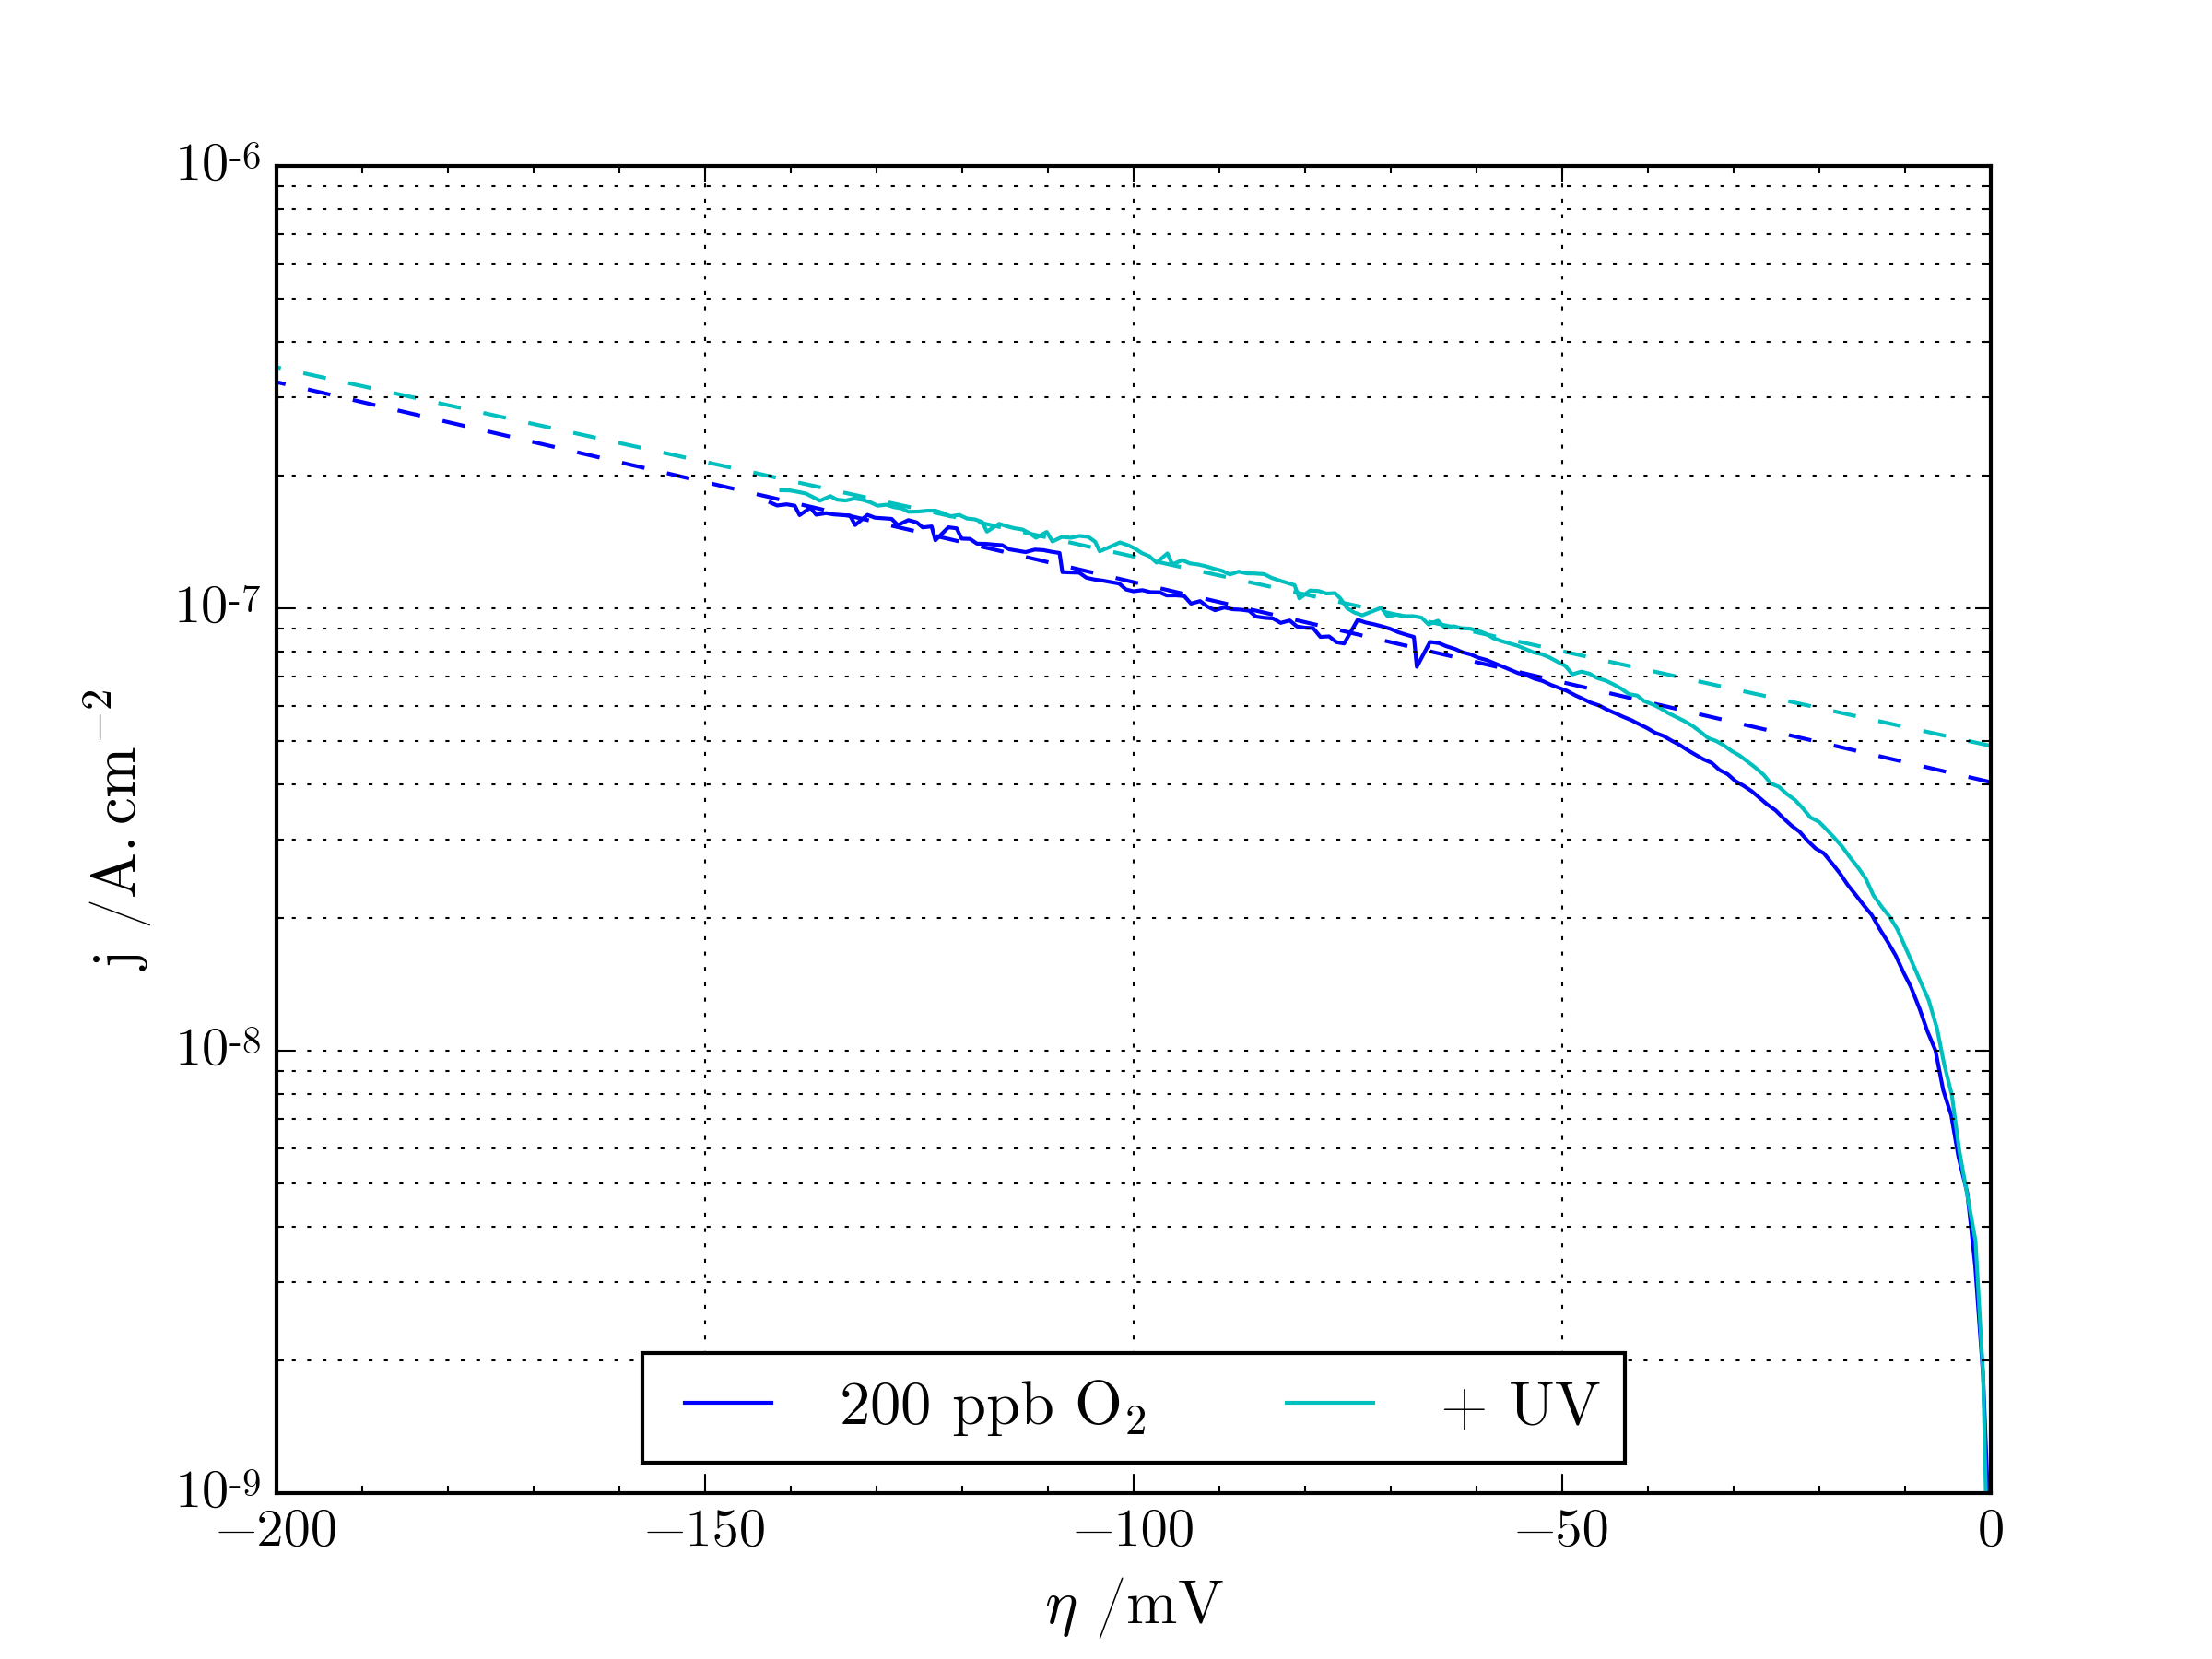
\includegraphics[width=\textwidth]{150215-chap4-PD-Inc718-WE8-n-3.png}
                \caption{}
                \label{}
            \end{subfigure}
            \begin{subfigure}[b]{\localfigwidth}
                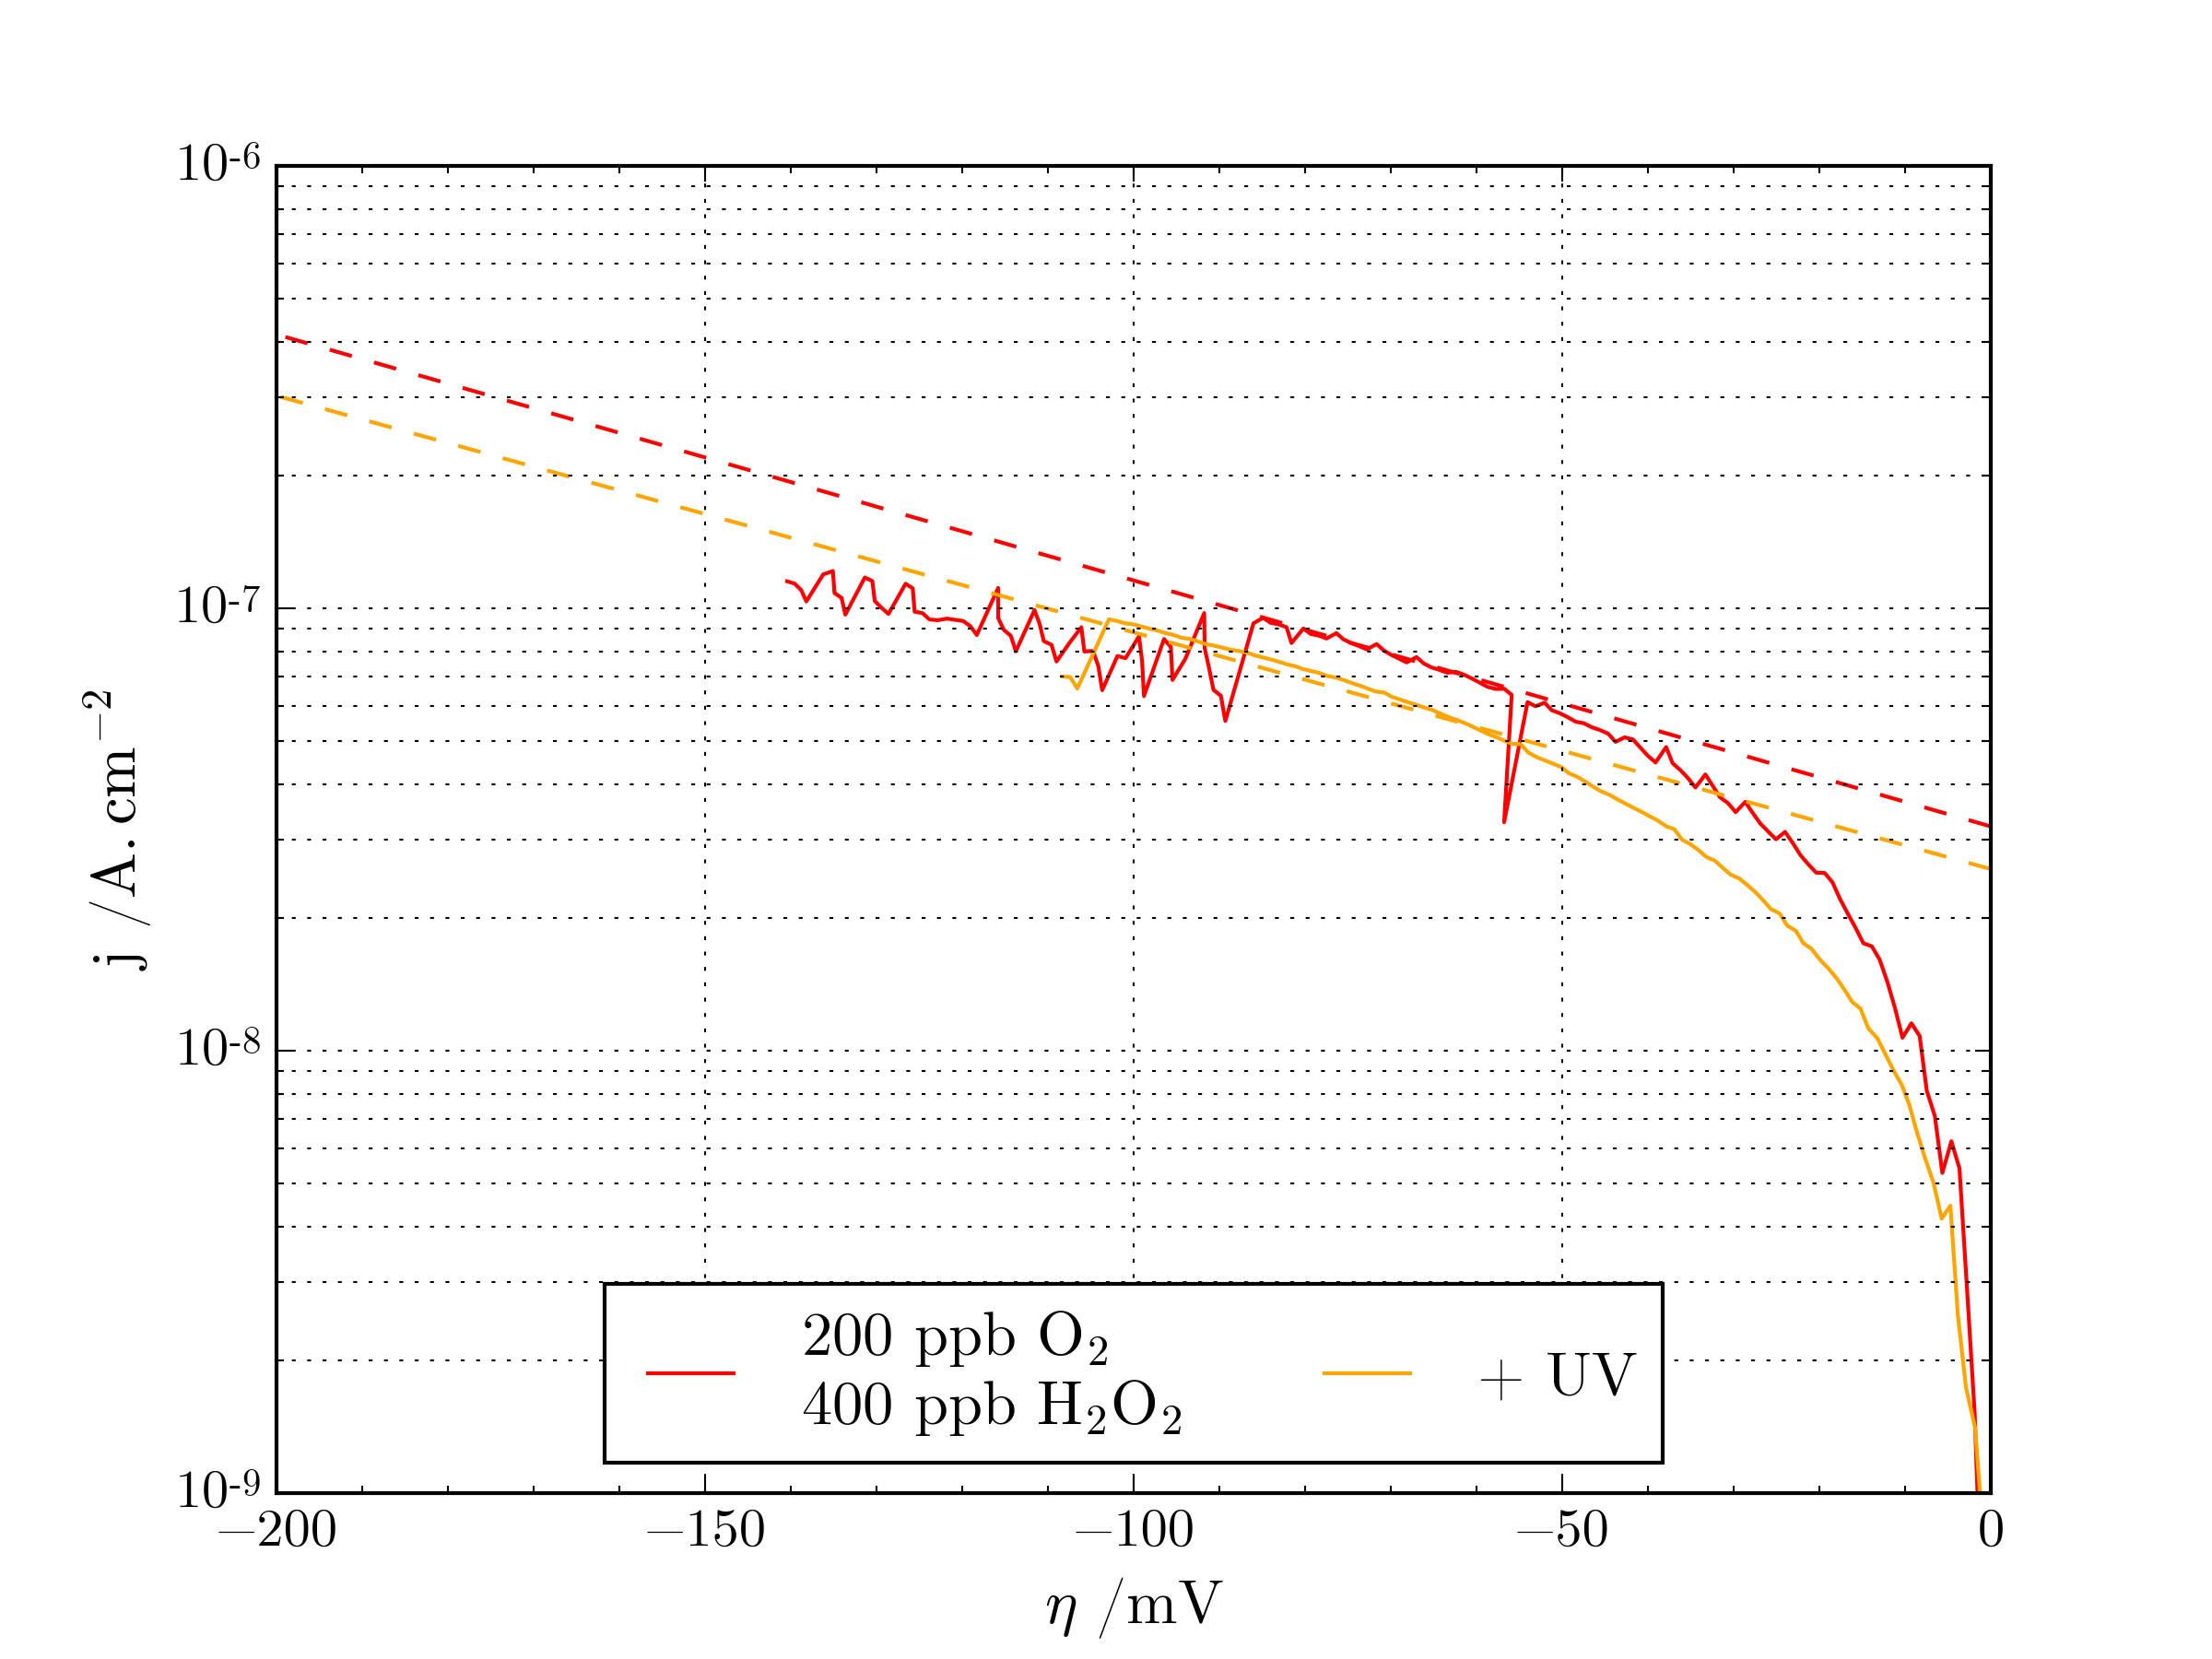
\includegraphics[width=\textwidth]{150215-chap4-PD-Inc718-WE8-n-5.png}
                \caption{}
                \label{}
            \end{subfigure}
            \caption{Evolution des densités de courant cathodique de l’échantillon Inc718, avec et sans illumination
            UV--Visible, en fonction de la surtension, pour les trois électrolytes considérés. a) Désaéré, b) 200 ppb
        d’oxygène, c) 200~ppb d’oxygène + 400~ppb de peroxyde d’hydrogène.}
            \label{fig:ch4_718_Tafel}
    \end{figure}


    
    \subsection{Synthèse des résultats}\label{subsec:ch4_oxygen_summary}

    \subsubsection{Principales observations}\label{subsec:ch4_oxygen_summary_main}
    
    Dans les électrolytes considérés et pour les échantillons oxydés en micro-autoclave de notre étude, le potentiel
    électrochimique en circuit ouvert de l’échantillon d’Inc718 est toujours plus anodique que celui de l’échantillon de
    Zy2:
    le couplage galvanique des deux matériaux se traduit globalement par une réaction d’oxydation sur l’échantillon de Zy2
    et une réaction de réduction sur l’échantillon d’Inc718. A l’obscurité, le potentiel électrochimique à l’abandon de
    l’échantillon d’Inc718 évolue vers des valeurs plus anodiques en présence d’oxygène dissous ; c’est le cas aussi pour
    échantillon de Zy2, mais l’effet est moins prononcé.
    L’illumination UV--Visible entraîne, pour les deux matériaux, une
    diminution du potentiel électrochimique à l’abandon vers des valeurs plus cathodiques, diminution d’amplitude plus
    importante en présence de peroxyde d’hydrogène. Cette diminution photo-induite du potentiel en circuit ouvert signe un
    comportement semiconducteur global des couches d’oxydation de type \emph{n}. 

    Quel que soit l’électrolyte considéré, le couplage des échantillons oxydés d’Inc718 et de Zy2 se traduit par un courant
    circulant dans le sens de l'oxydation sur l’échantillon de Zy2 et de la réduction sur l’échantillon
    d’Inc718. Egalement dans tous les électrolytes, la densité de courant de couplage d’Inc718 augmente lors de la première
    transition obscurité/illumination UV--Visible, d’un facteur égal à environ 5, impliquant une augmentation potentielle de
    la corrosion du Zy2, mais de manière peu différenciée selon les électrolytes, car, contrairement à ce qui a été observé
    pour les photopotentiels, la présence dans l’électrolyte de peroxyde d’hydrogène en plus de l’oxygène ne semble pas
    avoir un impact majeur sur la densité de courant de couplage avec et sans illumination UV--Visible. Par ailleurs,
    l’extrapolation des courants de couplage mesurés dans nos conditions d’illumination conduit à des valeurs de courants
    compatibles avec celles qu’impliquent la Shadow Corrosion en conditions réelles. De plus, l’évolution de la charge
    échangée en fonction du temps pendant les phases d’illumination semble indiquer un possible effet de la vitesse
    d’écoulement de l’électrolyte sur l’apport des espèces redox à la surface des échantillons. La réalité de cet effet
    reste à vérifier expérimentalement.
    
    
    Dans nos conditions expérimentales, l’illumination UV--Visible ne semble pas modifier, par rapport à la situation
    d’obscurité, les valeurs des coefficients de transfert telles que déterminées à partir des courbes de polarisation,
    mais semble seulement modifier les densités de courant d’échange de l’alliage Zy2.

    Il apparaît donc que l’effet des conditions d’électrolyte sur le comportement électrochimique des échantillons n’est
    pas simple à appréhender. Pour tenter de clarifier cette question, dans le paragraphe suivant, nous nous proposons
    d’examiner quelles réactions électrochimiques peuvent être envisagées sur les deux échantillons de Zy2 et Inc718 en
    fonction des couples redox présents dans l’électrolyte, moyennant bien sûr quelques hypothèses simplificatrices.
    
    \subsubsection{Réactions électrochimiques envisageables sur les échantillons de Zy2 et Inc718}
    \label{subsec:ch4_oxygen_summary_reactions}

    Nous avons vu au paragraphe \ref{subsec:post_mortem_PEC} que la caractérisation PEC post-mortem des échantillons de Zy2 et Inc718, couplés et
    exposés en eau ultra-pure, montre que les couches d’oxydes sont composées de différentes phases à propriétés
    semiconductrices (tableaux \ref{tab:ch4_band_gaps_fit_718} et \ref{tab:ch4_band_gaps_fit_Zy2}).
    Etant donné que nous n’avons pas pu caractériser par photoélectrochimie
    les échantillons non couplés, nous faisons ici l’hypothèse que les phases présentes dans les échantillons non couplés
    sont similaires à celles constituant les couches d’oxydation des échantillons couplés. Mais cette hypothèse reste à
    vérifier expérimentalement.

    Lorsque l’on souhaite examiner les réactions électrochimiques susceptibles d’être favorisées ou défavorisées à une
    interface entre un semiconducteur donné et un électrolyte donné, il est nécessaire de s’intéresser aux positions
    relatives en énergie, d’une part des bords de bandes de valence et de conduction en surface du semiconducteur,
    $E_{vs}$  et $E_{cs}$
    respectivement, et d’autre part des niveaux énergétiques électroniques les plus probables des états OX et RED,
    respectivement $E^{\circ}_{OX}$ et $E^{\circ}_{RED}$, des couples redox présents dans l’électrolyte. En effet, selon une approximation
    communément acceptée dans la littérature et assez bien vérifiée expérimentalement dans des cas simples
    \citep{Memming2008, Morrison1980, Gerischer1989, Gomes1973},
    le transfert de charge à une interface semiconducteur/électrolyte s’effectue de manière isoénergétique, aux
    niveaux d’énergie électroniques $E_{vs}$ et $E_{cs}$.

    La figure \ref{fig:ch4_isoE_transfert} illustre le principe d’un tel transfert de charge, pour un couple redox en conditions standard dans
    l’électrolyte en contact avec un semiconducteur de type \emph{n}. Dans cette figure, N(E) représente la densité d’états
    disponibles à l’énergie E soit pour l’espèce RED, soit pour l’espèce OX. Cette densité d’états est le produit de la
    concentration de l’espèce RED ou OX par une probabilité d’existence d’un niveau d’énergie électronique localisé sur
    l’espèce RED ou OX à l’énergie E, notée P(E). La courbe P(E) est une gaussienne dont les paramètres caractéristiques
    sont, d’une part le niveau $E^{\circ}_{RED}$ (pour l’espèce RED) ou le niveau $E^{\circ}_{OX}$ (pour l’espèce OX), d’autre part une énergie dite
    de réorganisation de la sphère de solvatation, notée $\lambda _{RED}$ ou $\lambda _{OX}$ selon l’état considéré. Sauf solvatation très
    différente des espèces RED et OX et/ou adsorption en surface du semiconducteur de l’une et/ou l’autre des deux espèces,
    les valeurs de $\lambda _{RED}$ ou $\lambda _{OX}$ sont généralement considérées égales, à une valeur $\lambda$, typiquement 0.75~eV 
    en milieu aqueux \citep{Gomes1973}.

    En bref, dans ce modèle de transfert de charge, et pour des semiconducteurs de gaps supérieurs à environ $2\lambda$, on peut
    considérer pour un semiconducteur de type \emph{n} que les courants de réduction obtenus seront proportionnels au produit de la
    densité d’électrons en surface du semiconducteur à l’énergie $E_{cs}$ (fonction du type de semiconduction, du taux de dopage
    et du potentiel appliqué) et de la densité d’états OX à l’énergie considérée. Et que les courants d’oxydation obtenus
    seront proportionnels au produit de la densité de trous en surface du semiconducteur à l’énergie $E_{vs}$
    (potentiellement importante sous illumination adéquate) et de la densité d’états RED à l’énergie considérée.

    \begin{figure}[H]
        \centering
        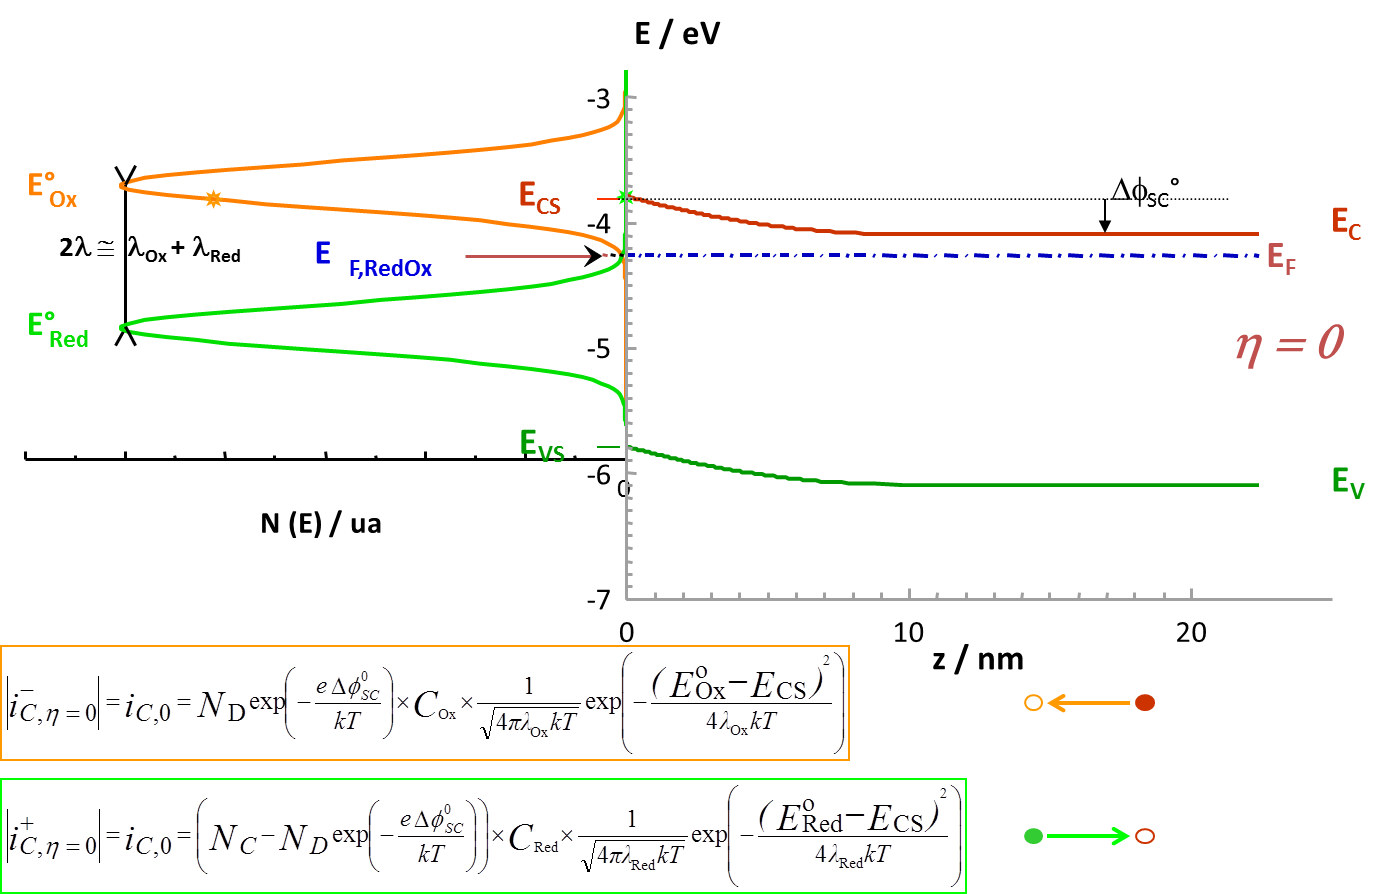
\includegraphics[width=\textwidth]{Petit-Transfert.png}
        \caption[Exemple de transfert électronique isoénergétique entre un couple redox et le niveau d’énergie de
        surface de la bande de conduction pour un semiconducteur de type \emph{n}.]
        {Exemple de transfert électronique isoénergétique entre un couple redox et le niveau d’énergie de
        surface de la bande de conduction pour un semiconducteur de type \emph{n} d’après \citep{Petit2010}.}
        \label{fig:ch4_isoE_transfert}
    \end{figure}

    Dans le travail effectué ici, nous nous sommes exclusivement intéressés au
    second terme de ces produits donné par l'équation \ref{eq:ch4_Pox_Pred}. Nous avons
    évalué, aux énergies $E_{cs}$ et $E_{vs}$ des divers semiconducteurs rencontrés dans notre étude, la probabilité d’existence de
    niveaux énergétiques électroniques localisés sur les états RED et OX de divers couples redox. Autrement dit, nous avons
    calculé la probabilité, $P_{OX}(E=E_{cs})$, d’injecter un électron de la bande de conduction vers l’oxydant et la probabilité,
    $P_{RED}(E=E_{vs})$, d’injecter un électron du réducteur vers la bande de valence. 

    \begin{equation}
        \begin{split}
            P_{OX}(E) &= \frac{1}{\sqrt{4\pi \lambda _{Ox}kT}}\exp \left[ -\frac{(E_{OX}^{\circ}-E_{cs})^2}{4\lambda
        _{OX} kT}
        \right] \\
        P_{RED}(E) &= \frac{1}{\sqrt{4\pi \lambda _{Red}kT}}\exp \left[ -\frac{(E_{RED}^{\circ}-E_{vs})^2}{4\lambda
    _{RED} kT}
        \right] \\
        \end{split}
        \label{eq:ch4_Pox_Pred}
    \end{equation}

    Les niveaux énergétiques $E_{cs}$ et $E_{vs}$ ont été déterminés en utilisant l’approche thermodynamique de Butler
    et Ginley
    \citep{Butler1978},
    basée sur la définition de Sanderson de l’électronégativité d’un solide, qui permet de calculer ces niveaux pour un pH
    égal au pzc. Mais nous avons ensuite corrigé les valeurs ainsi obtenues de l’écart entre le pzc du matériau et le pH de
    notre électrolyte (estimé à 5.5) pour une température de \SI{280}{\degreeCelsius} selon la relation \ref{eq:ch4_Ecs_vs_pH}
    \citep{Morrison1980}. Il convient toutefois de
    mentionner que nous ne disposions que de valeurs de pzc à \SI{20}{\degreeCelsius} \citep{Kosmulski2009}. 


    \begin{equation}
        E_{cs} = E_{cs}^{pH=pzc} + 2.3kT(pzc-pH)
        \label{eq:ch4_Ecs_vs_pH}
    \end{equation}    

    Nous avons considéré d’une part, les phases semiconductrices $ZrO_2$, $Cr_2O_3$, $Fe_2O_3$, $SnO_2$, et $Nb_2O_5$
    (mentionnées dans les
    tableaux \ref{tab:ch4_band_gaps_fit_718} et \ref{tab:ch4_band_gaps_fit_Zy2}),
    d’autre part les couples redox $H_2/H^+$, $H_2O/O_2$, $H_2O/OH^{\bullet}$,
    $H_2O_2/O_2$, $H_2O/H_2O_2$. 
    Le tableau \ref{tab:ch4_probabilities_oxidation} ainsi que le tableau \ref{tab:ch4_probabilities_reduction} 
    présentent les valeurs obtenues pour $P_{OX}(E=E_{cs})$ et $P_{RED}(E=E_{vs})$ pour les interfaces
    correspondantes; la figure \ref{fig:ch4_pos_RED_OX} illustre les positionnements relatifs
    des probabilités d’existence des états RED et OX
    des cinq couples redox  par rapport aux énergies $E_{vs}$ et $E_{cs}$ des cinq semiconducteurs.

    \begin{table}[H]
        \centering
        \rowcolors{2}{}{lightgray}
        \begin{tabular}{p{0.12\textwidth}|%
                        >{\centering\arraybackslash}p{0.13\textwidth}%
                        >{\centering\arraybackslash}p{0.13\textwidth}%
                        >{\centering\arraybackslash}p{0.13\textwidth}%
                        >{\centering\arraybackslash}p{0.13\textwidth}%
                        >{\centering\arraybackslash}p{0.13\textwidth}%
                    }

        \toprule
         &  $H_2/H^+$ &  $H_2O/O_2$ &  $H_2O/OH^{\bullet}$ &  $H_2O_2/O_2$ &  $H_2O/H_2O_2$ \\
        \midrule
        $ZrO_2$      &          0 &           0 &                 0 &             0 &           0 \\\hline
        $Cr_2O_3$    &          0 &           0 &                 \textcolor{red}{0.96} &             0 &           0 \\\hline
        $Fe_2O_3$    &          0 &           0 &                 \textcolor{red}{0.71} &             0 &           0.01 \\\hline
        $SnO_2$      &          0 &           0 &                 0.05 &             0 &           0 \\\hline
        $Nb_2O_5$    &          0 &           0 &                 \textcolor{red}{0.40} &             0 &           0 \\
        \bottomrule
        \end{tabular}
        \caption{Valeurs estimées de la probabilité, $P_{RED}(E=E_{vs})$, d’injecter un électron de l’état RED vers la bande de
        valence à l’énergie $E_{vs}$ pour les différents couples redox et semiconducteurs considérés.}
        \label{tab:ch4_probabilities_oxidation}
    \end{table}


    \begin{table}[H]
        \centering
        \rowcolors{2}{}{lightgray}
        \begin{tabular}{p{0.12\textwidth}|%
                        >{\centering\arraybackslash}p{0.13\textwidth}%
                        >{\centering\arraybackslash}p{0.13\textwidth}%
                        >{\centering\arraybackslash}p{0.13\textwidth}%
                        >{\centering\arraybackslash}p{0.13\textwidth}%
                        >{\centering\arraybackslash}p{0.13\textwidth}%
                    }

        \toprule
        &  $H^+/H_2$ &  $O_2/H_2O$ &  $OH^{\bullet}/H_2O$ &  $O_2/H_2O_2$ &  $H_2O_2/H_2O$ \\
        \midrule
        $ZrO_2$      &       \textcolor{red}{0.29} &        0.01 &                 0 &          \textcolor{red}{0.61} &           0 \\\hline
        $Cr_2O_3$    &       0 &        \textcolor{red}{1} &                 0 &          \textcolor{red}{0.13} &\textcolor{red}{0.11} \\\hline
        $Fe_2O_3$    &       0 &        0.01 &                 0.03 &          0 &           \textcolor{red}{0.53} \\\hline
        $SnO_2$      &       0 &        \textcolor{red}{0.69} &                 0 &          \textcolor{red}{0.49} &           0.01 \\\hline
        $Nb_2O_5$    &       0 &        \textcolor{red}{1} &                 0 &          \textcolor{red}{0.13} &\textcolor{red}{0.11} \\
        \bottomrule
        \end{tabular}
        \caption{Valeurs estimées de la probabilité, $P_{OX}(E=E_{cs})$, d’injecter un électron de la bande de
            conduction à l'énergie $E_{cs}$ vers
        l’état OX pour les différents couples redox et semiconducteurs considérés.}
        \label{tab:ch4_probabilities_reduction}
    \end{table}

    Le tableau \ref{tab:ch4_probabilities_oxidation} montre que la photo-oxydation de l’eau sur la zircone est très peu probable, car le niveau énergétique de
    la bande de valence de $ZrO_2$ est très éloigné du niveau $E^{\circ}_{RED}$ du couple $OH^{\bullet}/H_2O$.
    Par contre, la photo-oxydation de l’eau
    en radical $OH^{\bullet}$ est, toutes choses égales par ailleurs, très favorisée sur les phases semiconductrices chromine et
    hématite, et, à un degré moindre sur l’oxyde de niobium. Il en va sensiblement de même pour $FeCr_2O_4$ et des solutions
    solides de type $Fe_xCr_{2-x}O_3$ : ainsi, pour le couple $H_2O/OH^{\bullet}$, $P_{OX}(E=E_{cs})$ vaut 0.56 pour
    $FeCr_2O_4$, et vaut 0.74 pour $Fe_xCr_{2-x}O_3$ avec
    x=1. Notons en outre que les radicaux $OH^{\bullet}$ ainsi formés peuvent se recombiner en peroxyde
    d’hydrogène \citep{Trupin-Wasselin2000}. 

    Le tableau \ref{tab:ch4_probabilities_reduction}  montre que la réduction du proton en hydrogène n’est très favorisée
    que sur la zircone, et que la
    réduction de l’oxygène en eau est favorisée sur la chromine et sur les oxydes de niobium et d’étain. La réduction du
    peroxyde d’hydrogène en $H_2O$ est très probable sur l’hématite, un peu plus que sur la chromine et l’oxyde de niobium. On
    notera également que la réduction de l’oxygène en peroxyde d’hydrogène n’est très défavorisée que sur l’hématite. On
    peut penser que l’ajout de peroxyde d’hydrogène à l’eau pure contenant déjà de l’oxygène dissous défavorisera cette
    réduction de l’oxygène en peroxyde d’hydrogène, ce qui pourrait expliquer pourquoi le courant de couplage n’est pas
    significativement plus élevé lorsque l’oxygène dissous se trouve en combinaison avec le peroxyde d’hydrogène.

    L’information la plus importante apportée par les calculs présentés ci-dessus est que la photogénération de radicaux
    $OH^{\bullet}$
    est très favorisée sur l’hématite et la chromine. En effet, nous avons vu au chapitre \ref{chap:ch1_bib} (\S \ref{subsubsec:charge_carrier})
    que les dépôts rouges sur
    les gaines et les grilles de maintien, appelés CRUD (voir figure \ref{fig:what_is_shadow_corrosion}), sont majoritairement composés d’hématite et
    présente une certaine porosité. Par conséquent, le CRUD apparaît comme un danger potentiel pour la  résistance à la
    corrosion du Zy2, car il permettrait sous illumination la génération de radicaux très oxydants près de la surface de la
    gaine susceptibles d’entraîner la dissolution de la zircone selon un mécanisme tel que celui proposé par  \citet{Nishino1997} dans le cas
    d’$O_2^{-}$.
    Ce phénomène qui pourrait être amplifié par un couplage avec l’inconel favorisant l’évacuation
    des électrons vers ce dernier.

    Jusqu’à présent, dans ce chapitre, nous n’avons présenté, en termes de caractérisations photo-électrochimiques, que des
    essais post mortem menés à température ambiante, dont les résultats ont été utilisés dans ce paragraphe pour envisager
    les réactions électrochimiques favorisées ou défavorisées possibles sur les échantillons oxydés en micro-autoclave de
    Zy2 et Inc718. Dans le paragraphe suivant, nous présentons nos premiers résultats de caractérisations
    photoélectrochimiques en réacteur REB simulé, à 280°C.

     \begin{figure}[H]
        \centering
        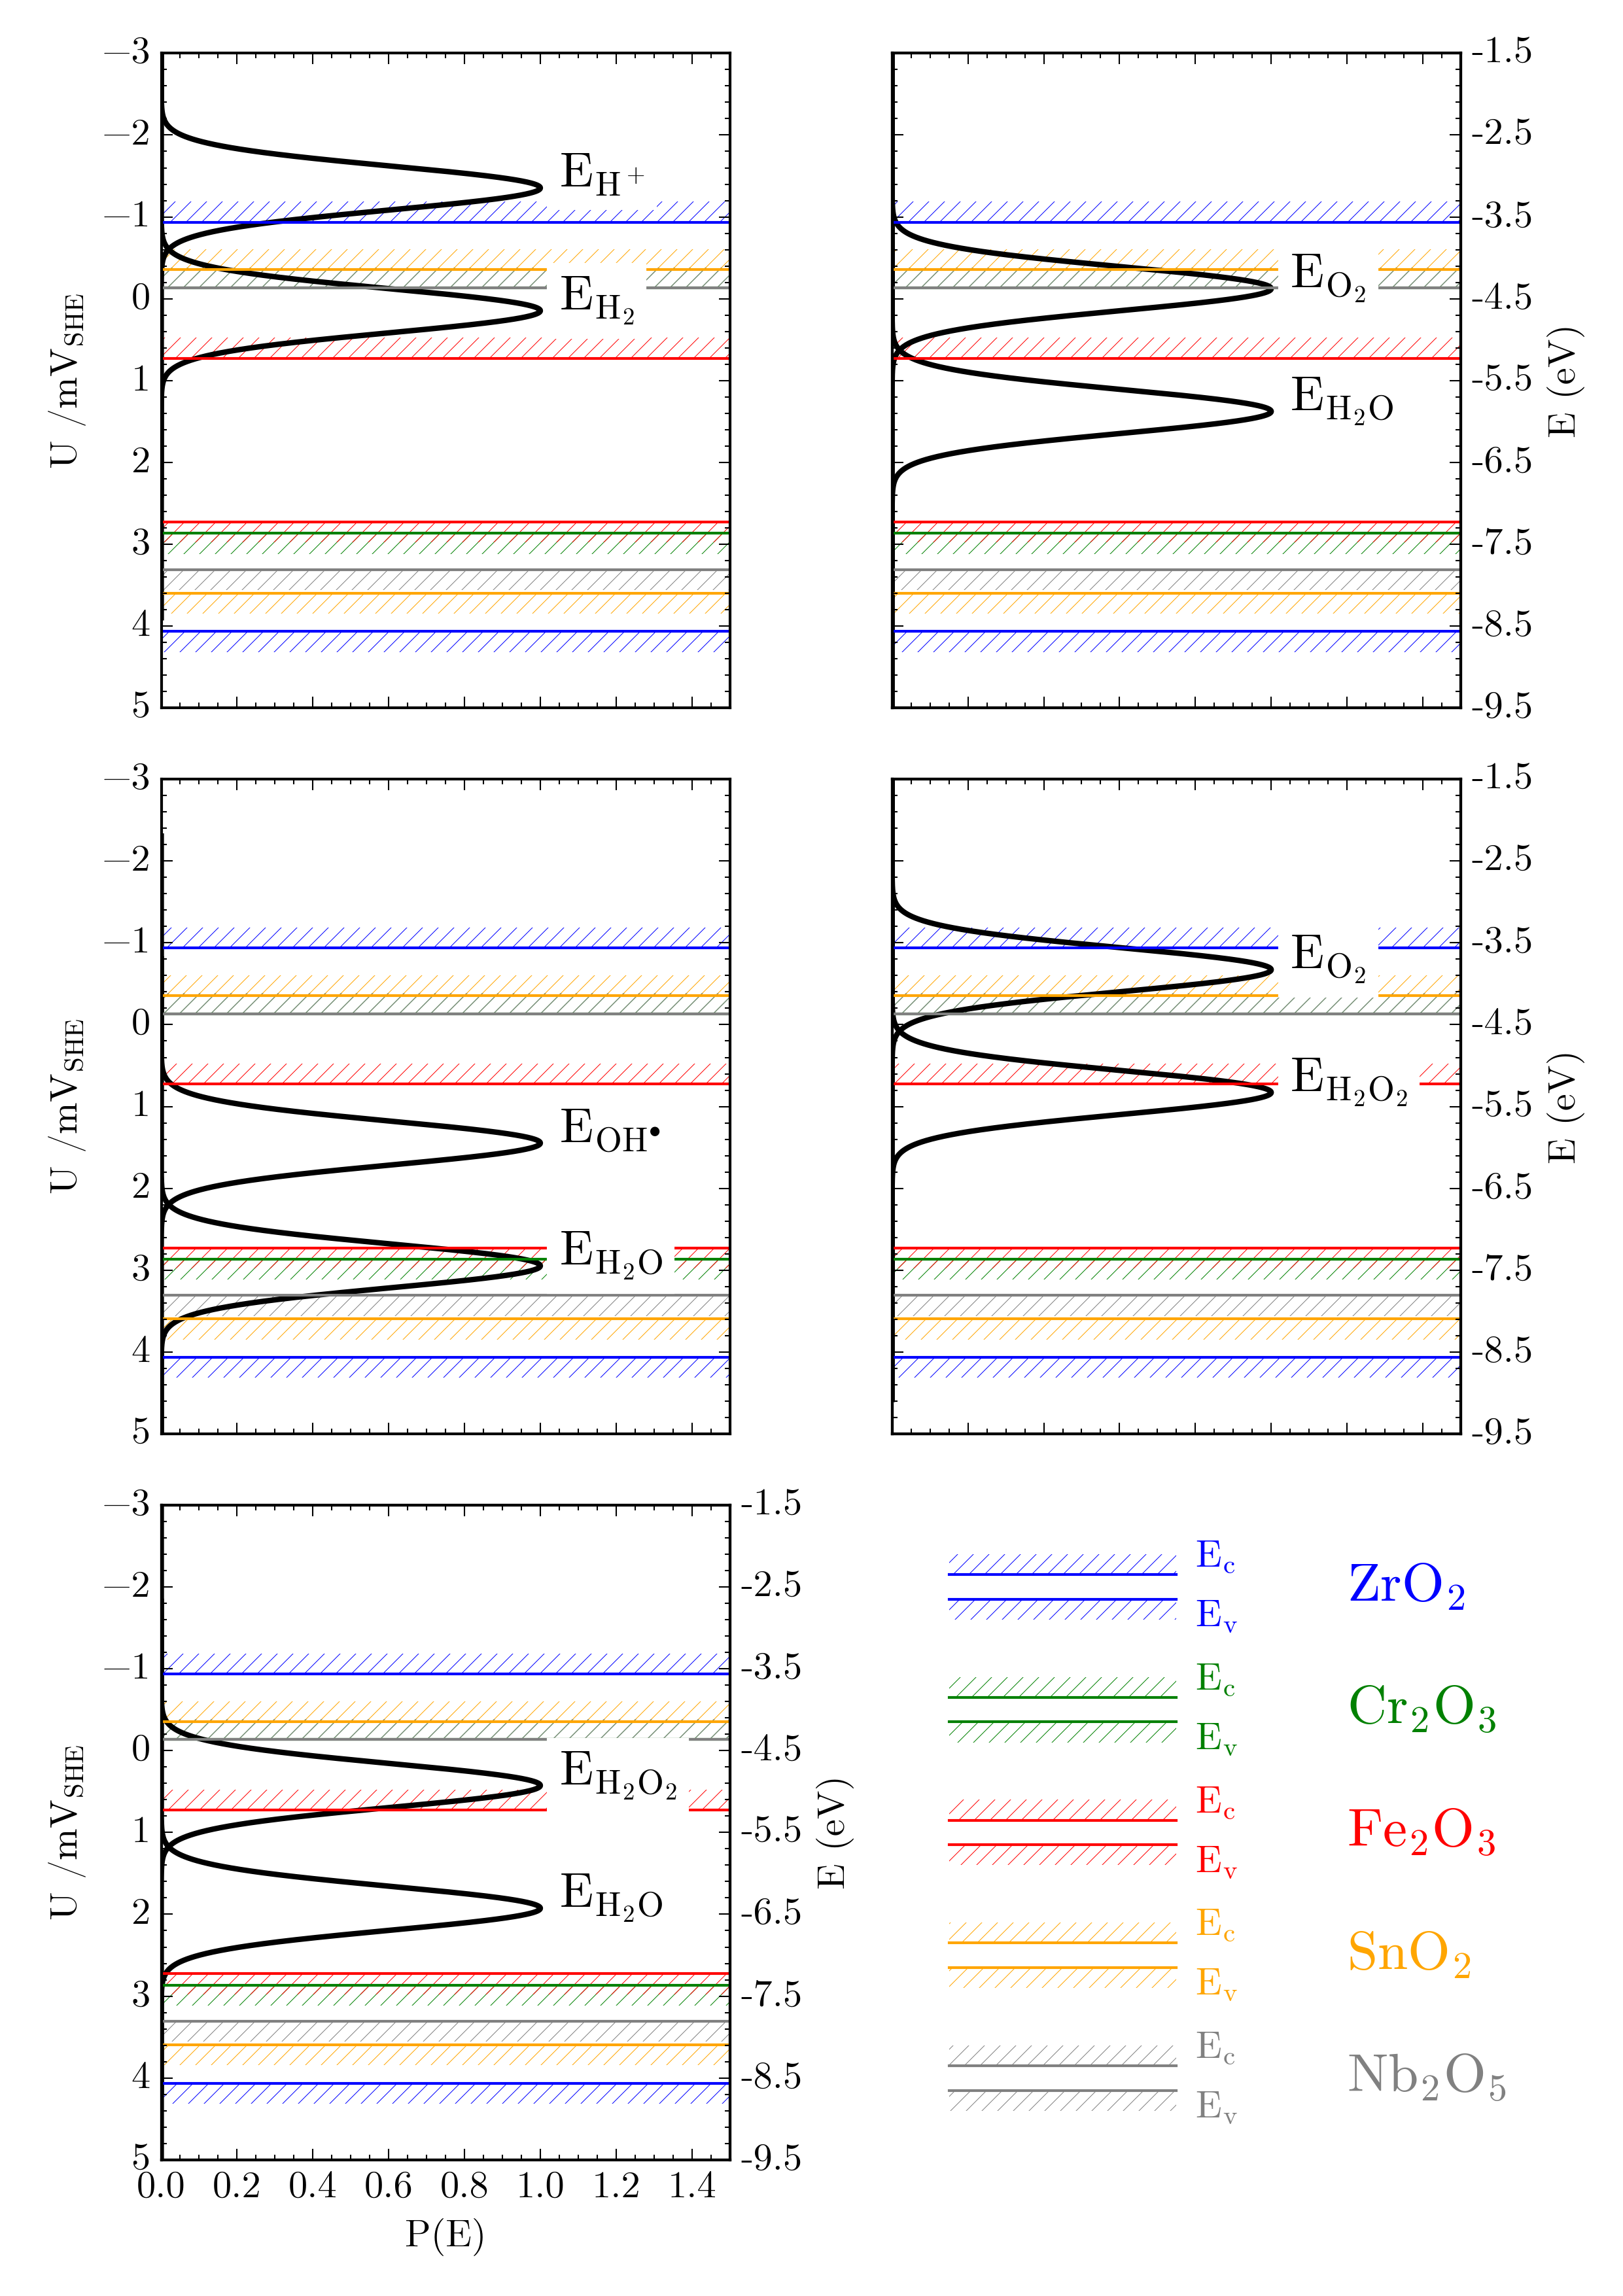
\includegraphics[width=\textwidth]{Band_Positions-All.png}
        \caption{Positionnements relatifs des niveaux d’énergie $E_{vs}$ et $E_{cs}$  et des probabilités d’existence de niveaux
        électroniques localisés sur les espèces RED et OX pour les semiconducteurs et couples redox considérés.}
        \label{fig:ch4_pos_RED_OX}
    \end{figure}

    


    \section{Caractérisation photo-électrochimique  \emph{in-situ} en cellule HTP}\label{sec:ch4_HT_PEC}


    La figure \ref{fig:ch4_HT_PEC_Zy2} illustre le premier spectre en énergie de photocourants obtenu dans la cellule HTP à 280°C sur
    l’échantillon de Zy2 préoxydé en eau ultra-pure (280°C, 80~bars). En raison de difficultés techniques liées à
    l’instrumentation, nous n’avons pas pu réaliser un spectre en énergie de photocourants à 280°C sur l’échantillon
    d’Inc718. Néanmoins, nous avons réalisé un spectre en énergie de photocourants sur un échantillon en alliage de
    nickel X750 également préoxydé en eau ultra-pure (280°C, 80 bars), spectre présenté en figure
    \ref{fig:ch4_HT_PEC_750}. Les spectres en
    énergie de photocourants obtenus à 280°C dans la cellule HTP sont comparés à ceux obtenus sur les mêmes échantillons
    à température ambiante dans le dispositif de caractérisation photoélectrochimique disponible au laboratoire SIMaP.
    Etant donné que les surfaces exposées à l’électrolyte ne sont pas les mêmes dans les deux dispositifs expérimentaux,
    les spectres en énergie de photocourants ont été normalisés à la surface exposée afin de pouvoir comparer les
    amplitudes du signal.

    Nous observons que l’amplitude du photocourant est plus importante à température ambiante par rapport aux amplitudes
    obtenues à 280°C notamment dans le cas de l’alliage de nickel X750. En effet, l’amplitude du photocourant est
    environ 2.5 et 50 fois plus élevée à température ambiante dans le cas de l’échantillon de Zy2 et X750,
    respectivement. Cette diminution de l’amplitude du photocourant à 280°C est très certainement liée à l’existence
    d’une conduction mixte dans la couche d’oxyde dont la conséquence est une "atténuation" du comportement de type
    diode de l’interface semiconducteur/électrolyte, comme déjà évoqué au paragraphe \ref{subsec:ch4_oxygen_Tafel} 
    lors de l’analyse des courbes
    de polarisation. En outre, le niveau de bruit sur les spectres en énergie de photocourants obtenus à 280°C dans la
    cellule HTP est relativement élevé, et notamment sur l’échantillon de Zy2. Ce niveau de bruit élevé n’a pas permis
    d’appliquer la procédure d’ajustement numérique abordée au chapitre 3 car les incertitudes associées aux paramètres
    ajustés étaient trop élevées.

    \begin{figure}[H]
        \centering
        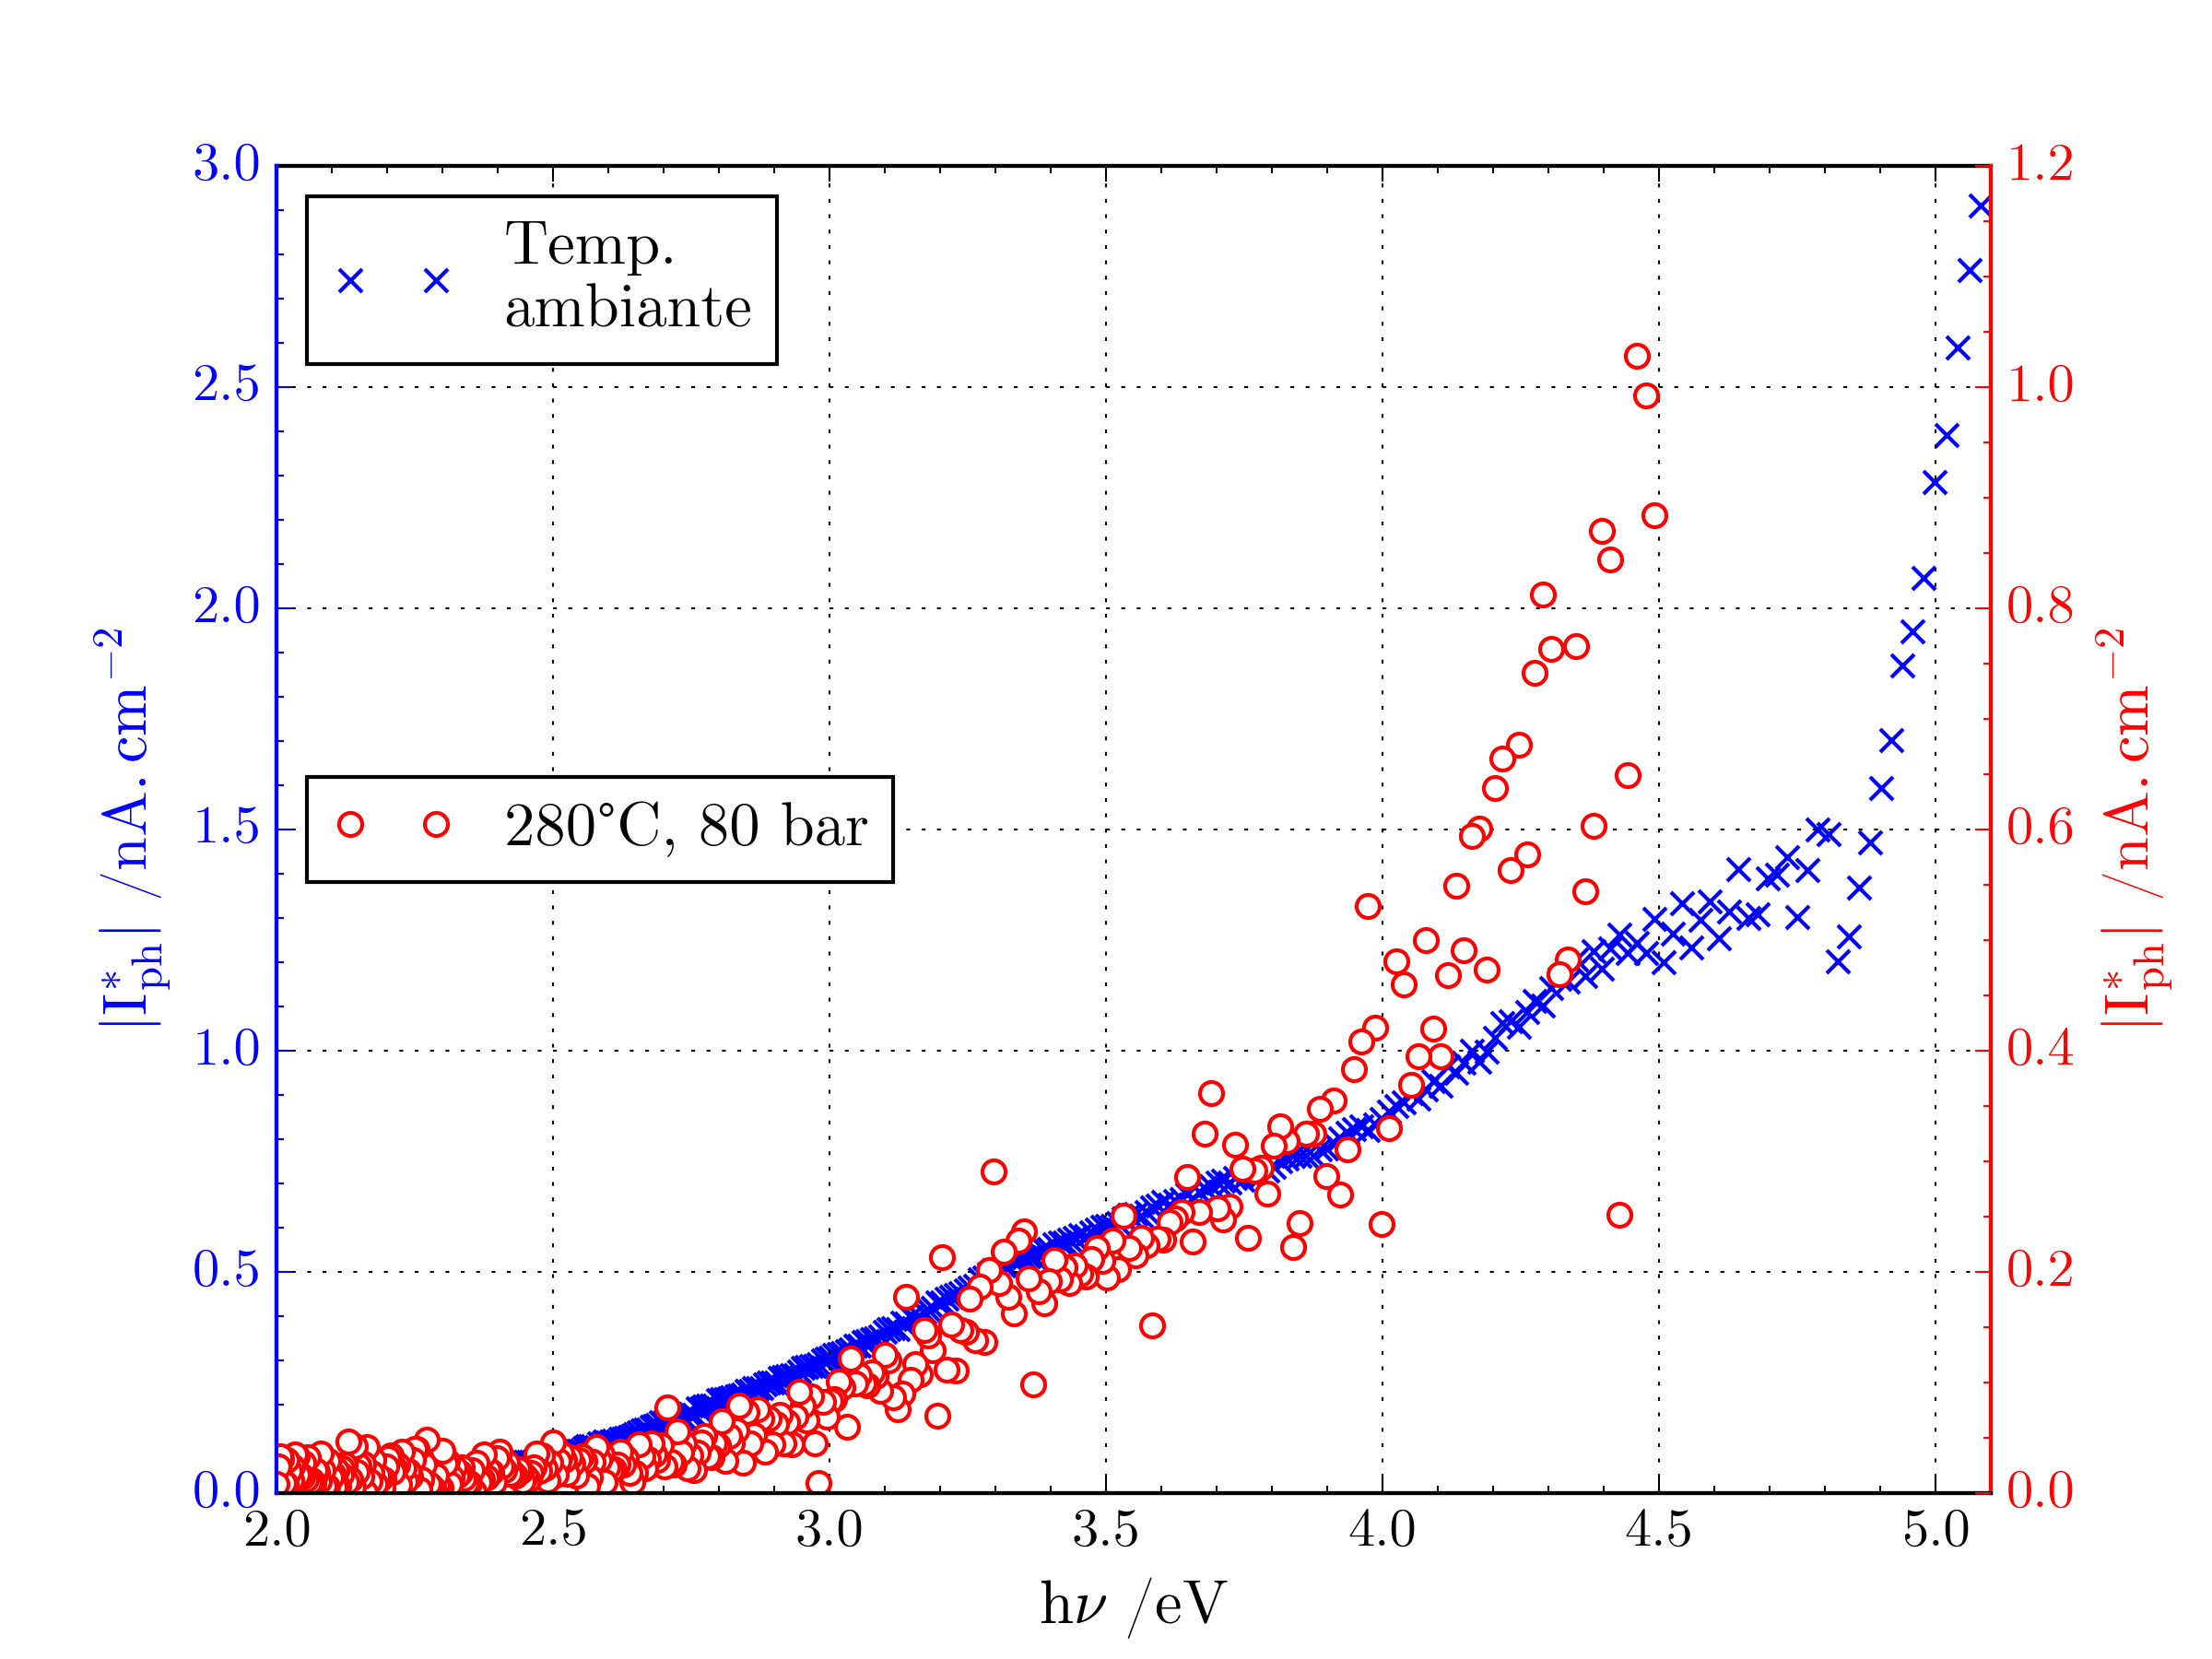
\includegraphics[width=\figwidth]{150215-chap4-PEC-Zy2-RT_HT-Iph.png}
        \caption{Spectres en énergie de photocourants obtenus sur l’alliage Zy2 oxydé (\SI{280}{\degreeCelsius} et
            \SI{80}{\bar} en eau ultra
        pure) avec le dispositif expérimental HTP développé dans ce travail.}
         \label{fig:ch4_HT_PEC_Zy2}
    \end{figure}

    \begin{figure}[H]
        \centering
        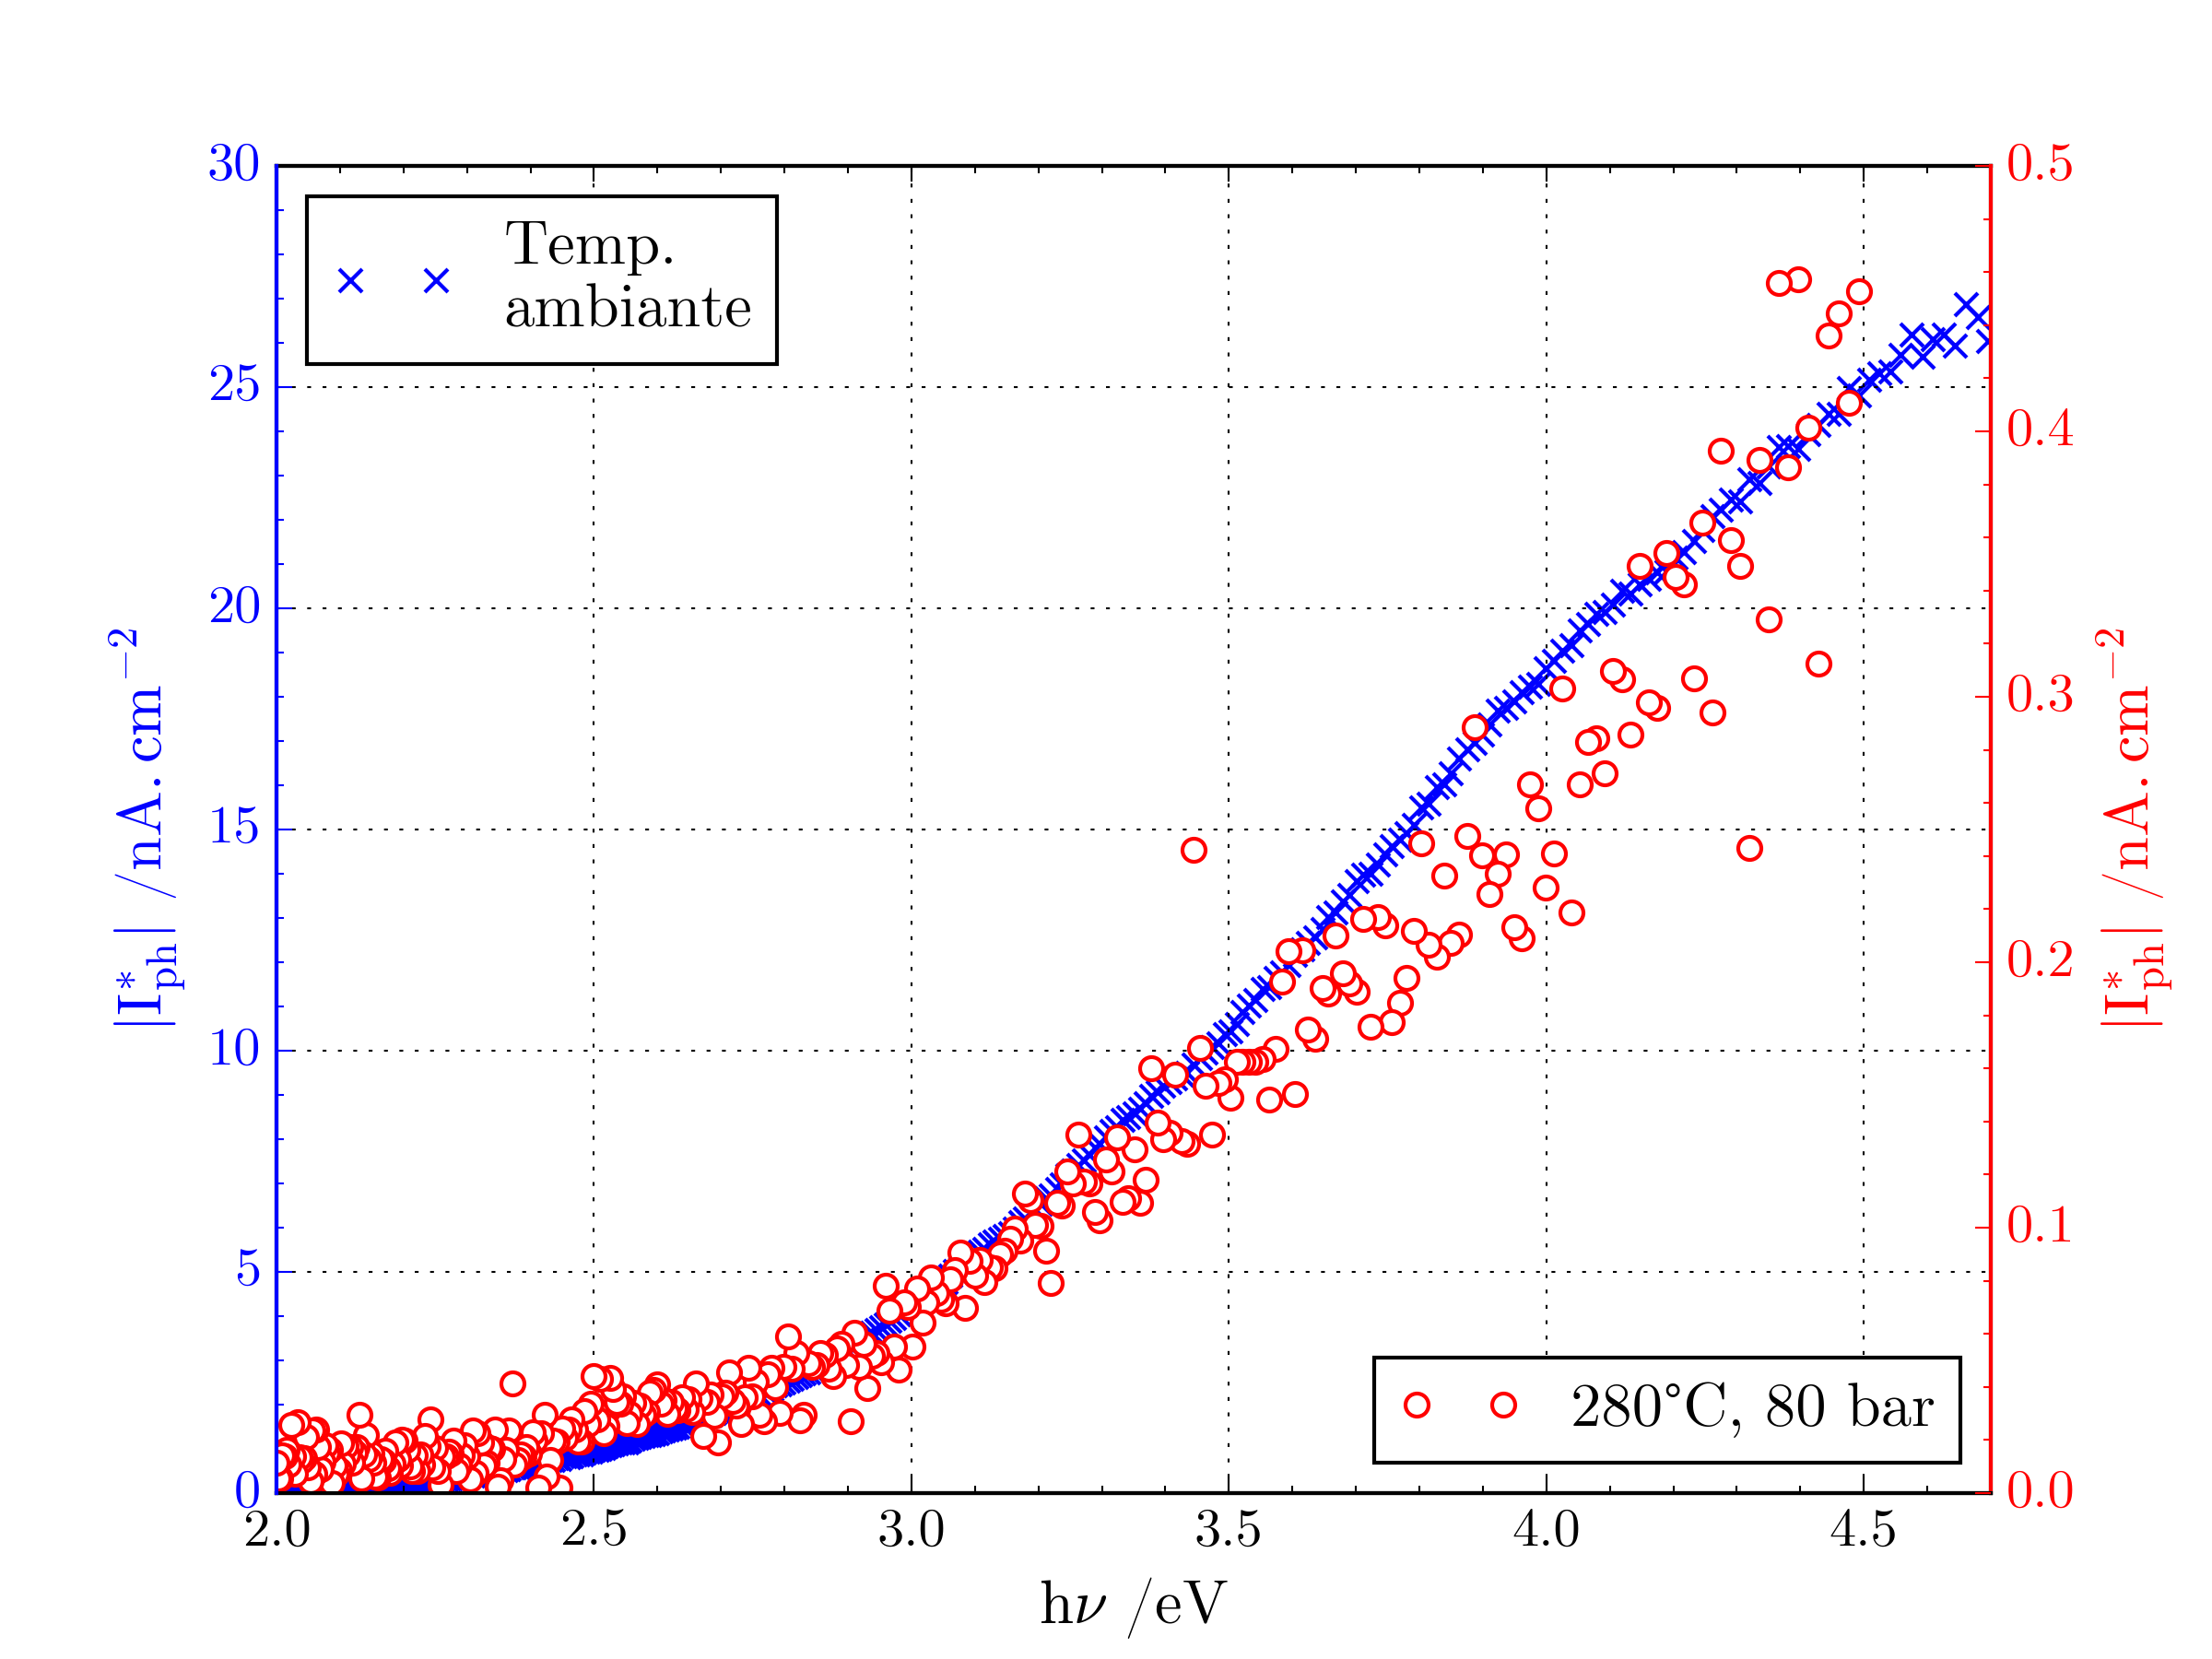
\includegraphics[width=\figwidth]{150888-chap4-PEC-X750-RT_HT-Iph.png}
        \caption{Spectres en énergie de photocourants obtenus sur l’alliage de nickel X750 oxydé ((\SI{280}{\degreeCelsius} et
            \SI{80}{\bar} en
        eau ultra pure) avec le dispositif expérimental HTP développé dans ce travail.}
        \label{fig:ch4_HT_PEC_750}
    \end{figure}


    Afin de mieux pouvoir comparer les allures des spectres en énergie de photocourants obtenus à température ambiante
    dans le dispositif du laboratoire SIMaP et à 280°C dans la cellule HTP, les spectres en énergie des figures
    \ref{fig:ch4_HT_PEC_Zy2} et \ref{fig:ch4_HT_PEC_750}
    ont été normalisés à 1 pour une énergie de 3.9~eV, et sont présentés ainsi en figures \ref{fig:ch4_HT_PEC_Zy2_Norm} et 
    \ref{fig:ch4_HT_PEC_750_Norm}.
    
    Nous pouvons observer que les spectres en énergie de photocourants à 280°C ressemblent fortement à ceux
    obtenus à température ambiante : les spectres en énergie de photocourants mesurés à température ambiante semblent
    passer par les points centraux du nuage des points mesurés à 280°C. 

    Notons en passant que la faiblesse relative du rapport signal/bruit s’explique en partie par le fait que, par
    rapport aux conditions des mesures PEC post-mortem, la plus grande surface d’échantillon exposée à l’électrolyte, et
    la température plus élevée de ce dernier dans la cellule HTP, impliquent des courants électrochimiques globaux plus
    élevés. Cela nous a contraint à réaliser nos mesures de photocourants HTP sur le calibre 1~$\mu A$ du potentiostat, alors
    que le calibre 100~nA aurait permis d’amplifier 10 fois le signal. 
    
    Néanmoins, bien que les premiers spectres obtenus soient bruités, leur existence nous semble montrer que la
    caractérisation PEC \emph{in-situ} peut offrir la possibilité de suivre l’évolution des couches d’oxyde
    \emph{in-situ} et en 
    "temps réel" durant l’exposition de différents alliages à 280°C dans la cellule HTP. Cependant, il sera nécessaire
    de travailler à l’optimisation de la focalisation du faisceau lumineux à la sortie du monochromateur et à minimiser
    le bruit parasite provenant de toute l’électronique autour de la cellule HTP, notamment celle des cartouches
    chauffantes. 
    
    Enfin, il faut rappeler que des caractérisations photoélectrochimiques à 280°C dans un électrolyte aussi peu
    conducteur que l’eau ultra-pure, telles que celles que nous avons pu obtenir, n’avait jamais été réalisées jusqu’à
    présent. 

    \begin{figure}[H]
        \centering
        \includegraphics[width=\figwidth]{{150215-chap4-PEC-Zy2-RT_HT-Norm_3.92}.png}
        \caption{Spectres en énergie de photocourants obtenus sur l’alliage Zy2 oxydé (\SI{280}{\degreeCelsius} et
            \SI{80}{\bar} en eau ultra
        pure) dissous avec le dispositif expérimental HTP développé dans ce travail. Les photocourants ont été
    normalisés à 1 à 3.9~eV.}
        \label{fig:ch4_HT_PEC_Zy2_Norm}
    \end{figure}

    \begin{figure}[H]
        \centering
        \includegraphics[width=\figwidth]{{150888-chap4-PEC-X750-Comparison_HT_RT-Norm_3.97}.png}
        \caption{Spectres en énergie de photocourants obtenus sur l’alliage de nickel X750 oxydé (\SI{280}{\degreeCelsius} et
            \SI{80}{\bar} en
        eau ultra pure) avec le dispositif expérimental HTP développé dans ce travail. Les photocourants ont été
    normalisés à 1 à 3.9~eV.}
        \label{fig:ch4_HT_PEC_750_Norm}
    \end{figure}


    \section{Conclusions}

    Dans ce dernier chapitre, nous avons étudié dans un premiers temps, en l’absence d’illumination UV--Visible des
    échantillons, l’effet de la présence d’impuretés dans l’eau ultra-pure sur la corrosion d’échantillons de Zy2 en
    situation de couplage avec des échantillons d’Inc718, aucun de ces échantillons n’ayant subi une préoxydation préalable.
    Dans un deuxième temps, nous avons étudié l’effet, sur le comportement d’échantillons de Zy2 et Inc718 ayant subi une
    préoxydation préalable, des teneurs en oxygène et peroxyde d’hydrogène dissous dans l’eau ultra-pure, en présence et en
    l’absence d’illumination UV--Visible. 

    En absence d’illumination UV--Visible, nous pouvons affirmer que la présence d’un couplage galvanique n’a pas d’effet
    notable sur la corrosion de l’alliage Zy2 en eau ultra-pure en l’absence d’impureté. Par contre, la présence de cations
    de fer dans l’électrolyte peut être néfaste pour la corrosion de l’alliage Zy2. De plus, un effet de synergie négative
    entre cations de fer et cations de nickel et de zinc est envisageable, aggravant la corrosion du Zy2 notamment quand le
    rapport molaire \ratio\ est supérieur à 2. Ce résultat expérimental va tout de même à l’encontre des
    conclusions du retour d’expérience de l’incident du réacteur KKL mais ce dernier est basé sur des oxydations en
    réacteur sous irradiation neutronique dont nous ne reproduisons pas les conditions.

    Toujours en absence d’illumination UV--Visible, le comportement de l’alliage de nickel 718 est plus sensible à la
    présence d’impuretés dans l’électrolyte, et notamment de cations de fer, car ces derniers favorisent la formation d’une
    spinelle supplémentaire de type $AB_2O_4$ telle que $FeCr_2O_4$, dans la couche d’oxydes, par rapport à une couche d’oxydes
    formée en eau ultra-pure. De plus, la couche d’oxydes formée en présence de cations de fer semble être plus dopée, donc
    plus conductrice, favorisant ainsi le couplage galvanique. Dans le cas de l’alliage Zy2, la présence d’impuretés ne fait
    pas apparaître de phase semiconductrice supplémentaire dans la couche d’oxydes mais la présence de nickel et/ou de zinc
    favorise la formation de phases dont la largeur de bande interdite est inférieure à 3.5~eV et potentiellement  plus
    conductrices.

    L’ensemble des résultats des mesures de courants de couplage en présence d’impuretés dans l’électrolyte, et en l’absence
    d’illumination UV--Visible, suggère que les cations de fer joueraient un rôle important dans la corrosion de l’alliage
    Zy2 en situation de couplage. Ce résultat est intéressant car les cations de fer, provenant de l’oxydation des pièces de
    structure d’un réacteur nucléaire, sont présents dans l’eau et peuvent se retrouver sous forme de dépôt de couleur rouge
    (appelés CRUD) sur les gaines de Zy2 ainsi que les grilles de maintien en alliage de nickel 718. Néanmoins,
    l’utilisation d’électrolytes avec des mélanges de cations de fer, nickel et zinc rend très difficile la séparation des
    effets de chaque cation à partir de nos résultats expérimentaux. 
    %Notons cependant que, une pollution au fluor à hauteur
    %de 10 ppm dans chaque micro-autoclave ayant été détectée, il sera nécessaire de réaliser des mesures complémentaires
    %afin de complètement valider les résultats évoqués ci-dessus.

    En présence d’illumination UV--Visible, les deux alliages Zy2 et Inc718 voient leur potentiel électrochimique évoluer
    vers des valeurs plus cathodiques que celles mesurées à l’obscurité, signant une semiconduction de type \emph{n}, que
    l’électrolyte contienne ou non de l’oxygène et/ou  du peroxyde d’hydrogène. De plus, l’illumination UV--Visible des
    échantillons entraîne une augmentation du courant de couplage d’un facteur égal à environ 5, impliquant une augmentation
    potentielle de la corrosion du Zy2, mais de manière peu différenciée selon que l’électrolyte contient ou non de
    l’oxygène et/ou  du peroxyde d’hydrogène. Notons que, par extrapolation des courants de couplage à des flux lumineux
    UV--Visible plus représentatifs des conditions de flux en situation de Shadow Corrosion en réacteur réel, nous obtenons
    des ordres de grandeur de courant de couplage compatibles avec les valeurs qu’implique le phénomène de Shadow Corrosion.
    Notre protocole expérimental pour ces mesures pourrait être mis à profit pour tester de manière relativement rapide en
    laboratoire diverses solutions d’atténuation du phénomène de Shadow Corrosion.


    L’illumination UV--Visible ne semble pas modifier, par rapport à la situation d’obscurité, les valeurs des
    coefficients de transfert telles que déterminées à partir des courbes de polarisation, mais semble seulement
    modifier les densités de courant d’échange de l’alliage Zy2. Le faible impact de l’illumination UV--Visible sur les
    coefficients de transfert est très certainement lié à la présence d’une conduction mixte dans les couches d’oxyde
    impliquant que le comportement de type diode de l’interface semiconducteur/électrolyte est "atténué".
    
    La caractérisation PEC \emph{in-situ} offre la possibilité de suivre l’évolution des couches d’oxyde en "temps réel"
    durant l’exposition de différents alliages à 280°C dans la cellule HTP, et ce malgré le bruit observable sur les
    premiers spectres mesurés. Ces derniers, qui  montrent des amplitudes de photocourant plus faibles à 280°C qu’à
    l’ambiante, semblent également confirmer l’hypothèse de l’effet de la conduction mixte sur "l’atténuation" du
    comportement de type diode à l’interface semiconducteur/électrolyte très certainement liée à une augmentation des
    pièges de recombinaisons. Enfin, il faut mentionner que des caractérisations photoélectrochimiques à 280°C dans un
    électrolyte aussi peu conducteur que l’eau ultra-pure n’avait jamais été réalisées jusqu’à présent. Néanmoins, un
    travail d’optimisation du rapport signal/bruit est encore nécessaire afin de pouvoir appliquer la procédure
    d’ajustement numérique des spectres en énergie de photocourants.
    
    A l’examen des résultats en termes d’effet des impuretés (effet important des cations de fer) et d’effet de
    l’illumination UV--Visible (augmentation des courants de couplage), obtenus de manière indépendante respectivement en
    micro-autoclaves et en cellule HTP, il nous semble qu’il serait intéressant d’étudier l’effet de ces deux paramètres
    en cellule HTP , par exemple par injection de cations de fer (éventuellement de nickel et de zinc) directement dans
    la cellule HTP. En effet, les calculs du paragraphe \ref{subsec:ch4_oxygen_summary_reactions}, avec lesquels nous avons examiné les réactions
    électrochimiques envisageables sur différentes phases semiconductrices, ont montré que la présence d’hématite peut
    favoriser fortement la formation de radicaux $OH^{\bullet}$ en présence d’illumination, par photo-oxydation de l’eau. De plus,
    la formation éventuelle d’un dépôt sur l’alliage Zy2 et/ou de nickel 718 pourrait être suivie en temps réel avec la
    technique de caractérisation photoélectrochimique.
    
    Enfin, il nous semble nécessaire de noter que l’ensemble des résultats obtenus dans ce travail repose principalement
    sur des mesures électrochimiques. Il conviendra bien sûr de les ré-examiner à la lumière des résultats d’autres
    techniques de caractérisations \emph{ex-situ}, telles que l’XPS, ou la spectroscopie Raman (lorsque les couches d’oxydation
    formées sont suffisamment épaisses).

\singlespacing
\printbibliography[heading=subbibintoc]
\onehalfspacing
\end{refsection}
